% This file should be replaced with your file with an thesis content.
%=========================================================================
% Authors: Michal Bidlo, Bohuslav Křena, Jaroslav Dytrych, Petr Veigend and Adam Herout 2019
\chapter{Introduction}
\label{intro}

Assuring software quality is a crucial part of development cycles
for all kinds of software.
It is important for low-level code often deployed in highly critical
applications where one bug can have expensive consequences or even threat
human lives.
It is crucial also in~high-level software where~bugs can destroy
user experience and ruin the whole process of development and selling a new software.

\subparagraph{Approaches to Software Quality}
There are different approaches to software quality at different stages of development cycle
with different quality warranties.
The most rigorous one is based on a formal specification of requirements
followed by deriving program from the specification or proving program
against the specification manually or with help of automated proof assistant.
This approach is present from the beginning of computer science and although it provides
the highest level of guarantee it has not became mainstream.
The main negatives are the demands on qualification of developers and severe difficulties to scale
to larger software.

There are also more or even fully automated approaches to proving correctness of~programs such as
model checking which strive to verify that a program satisfies a given specification.
These methods are generally called formal verification.
They are easier to use than manual proving of program, however, they still have problems with scaling and applicability to real-world software.
There are more specialized automated methods such as different types of sound static analysis based, e.g., on data flow analysis
or~abstract interpretation, which are designed to verify certain program properties
(such as values of integer variables or analyses of termination properties).
These methods scale better and can work out of the box.
However, they are less precise and often tuned for a particular program property. 

Another approach comes from programming language community claiming
that programming language itself should guide a programmer to write
software without bugs.
This is mostly achieved by static strong type systems which facilitate
encoding different program properties to the type system.
The advantage of this approach is that one does not need another technology and forces
programmers to write correct code.
On the other hand, the programming languages of this kind have a slow learning curve
and can be even unusable for certain programmers.
Moreover, only a limited set of program properties is encodable to type systems.

The third approach to software quality are lightweight automated methods
such as automated testing, unsound static analysis based, e.g., on error pattern matching, symbolic execution,
or extrapolating dynamic analysis.
This class of methods also contains the relaxed versions of methods from formal verifiction
such as bounded model checking or different approaches to abstract interpretation which
do not overapproximate the original semantics.
The methods try to hit a sweet spot between mathematical rigour and plain bug hunting.
They are easy to use, straightforward, often scale well but may detect many false alarms which can cause
that they are ignored by developers completely.

The last of the main approach is based on traditional testing by humans possible aided
by automated test execution, continuous integration, and the like.
It may be developers writing unit tests or the whole tester teams implementing the complex integration tests.
It is mostly known and time-tested approach, but it costs a lot of human resources and
does not give any guarantees about correctness.

The presented dichotomy does not pretend to be complete or exhaustive.
It tries to summarise the main approaches and give an overview of them.
In practice, the different approaches are combined, complement each other, and may
fall to different categories at the same time.
The proposed thesis focuses on automated formal methods (the first part of thesis)
and lightweight automated testing methods (the second part), which we used in a domain where scalability was required.

\subparagraph{Finite Automata}
The main uniting theme of the thesis is application of finite automata to
the fields of formal verification and automated testing.
Finite automata are a (syntactically) simple but powerful tool for representing regular languages. 
%Particulary, such languages may consists of e.g., regular strings (used in pattern matching applications
%such as lexical analysis in compilers or detection of malicious strings in security domains),
%regular structures such as list or trees (used in verification of programs manipulating
%dynamic data strucutre), or regular sequences of messages (used in modelling communication
%protocols).
Since their introduction in the 50s by Rabin and Scott \cite{rabin-scott}, they have been used in
various domains such as compilers, modelling of various kinds of systems,
design of digital circuits, natural language processing, speech recognition,
as well as in verification or testing of software and hardware.
Moreover, finite automata and their variations are widely studied in theoretical computer science either
from perspective of the decidable properties or complexity of algorithms for their manipulation.

Finite automata are mainly used to represent the various structures with reccurent patterns of substructures (we deliberately
do not use word regular to prevent confusion with meaning of the word in context of theory of formal languages). 
A classical application is language consisting of plain strings (used in pattern-matching applications
such as lexical analysis in compilers or detection of malicious strings in security domains).
A more sophisticated case arises when using regular language s containing sequences of messages
or generally objects with an inner structure, which is used, e.g., for modelling communication protocols.
In formal verification, there are also automata representing regular languages of infinite strings (so called Buchi automata),
which are used for verification of some properties requiring one to reason about infinite behaviours such as termination of a program.
Another kind of automata used in formal verification are tree automata that represent sets of trees.
These automata have been applied, e.g., to represent tree data structures (and even more complex structures defined over their tree backbones)
allocated on heap by a program.

In the applications of automata in this thesis, we need to perform operations such as testing language inclusion and equivalence
of two finite automata, testing emptiness of language of automaton or complementation of automaton.
All these properties are decidable but some of them have a high complexity,
e.g., complement has exponential complexity w.r.t. number of states of automaton, language inclusion and equivalence are PSACE-complete
(or even EXPTIME-c for nondeterministic tree automata).
Fortunately, efficient heuristics for the mentioned operations were introduced making
them computationally feasible in many practical cases TODO CITE.

As we mentioned above, we focus on applications of automata to two different fields.
The first one is shape analysis, i.e., static analysis of programs manipulating
dynamic data structures.
In shape analysis, we are interested in representing data structures allocated on the heap, such
as linked lists or trees, and verifying the operations properties such as absence of invalid memory
dereference, invalid memory free, or memory leaks.
Programs using dynamic data structures are a great fit for methods of formal verification since 
they are prone to the mentioned bugs and are written in programming
languages with manual memory management as C or C++ where memory management is fully within user's control.
At the same time, these programs are used in critical software such as kernels of operating systems.
Any bugs in them may affect many users and lead to expensive losses.
Therefore they need strong safety guarantees which can be provided by the methods with formal basis.

Our approach to shape analysis is based on forest automata and automata over graphs
(both extensions of tree automata) with a bounded tree width.
Both formalisms are able to represent a quite wide class of data structures that can be
allocated on the heap.
We employ a verification procedure to compute shape invariants for each program location.
In our case, a shape invariant is an automaton representing all possible states of heap.
Finally, we check that shape invariants imply that a given specification is fulfilled by the program
(usually checking absence of invalid dereferences, invalid frees or memory leaks).

The second field of application of automata in this thesis is automated software testing.
Particularly, we focus on testing of a manufacturing execution system (MES) in an environment of digital twins.
MES is critical software in controlling a factory where bugs may stop
the~production or even damage manufacturing machines.
Such bugs may be very expensive, and it is important to find as many of them as possible
before MES is deployed to a real factory.
Our approach analyses the behavior of the software used in a real factory, builds its models and then
generates tests for a digital twin of the factory which are applied, e.g., when a new version of the software is deployed
and the rest of factory emulated.

\section{Goals of the Thesis}
The first goal of this thesis is to improve the current tools and methods of shape analysis.
We aim to further develop the approach to shape analysis based on forest automata proposed in \cite{cav11,cav13}
and enhance it by
\begin{enumerate*}
  \item revisiting and improving its description,
  \item enhancing it by a mechanism of checking possible counterexamples and automated abstraction refinement,
  \item improving its tool support, particulary tool \forester, to make it able to compete on an international level.
\end{enumerate*}
We also attempt to find an alternative automata-based representation suitable for shape analysis
with the aim of cover the class of graphs with bounded tree width.

Futher we want to study possible alternatives to shape analysis based on forest automata.
We will focuse mainly on the following topics:
\begin{enumerate*}
  \item an alternative automata-based representation with the aim of cover the class of graphs with bounded tree width (taking inspiration from Courcelle theorem \cite{Courcelle}),
  \item exploring possibilities of shape analysis based on predicate logic, templates-based invariants, abstract domains, and SMT solving.
\end{enumerate*}

The second goal of the thesis is to apply automata to the field of testing, particularly
to testing manufacturing execution systems.
We want to create a novel approach combining automated test generation from
observed behaviour of a manufactory with testing in an environment of a digital twin
which will be orchestrated according to the tests we create.

\section{Overview of the Achieved Results}
\paragraph{Shape analysis}
The first of our results is an extension of shape analysis on forest automata by
spurious counterexample detection and predicate abstraction refinement published in \cite{vmcai17}.
Abstraction is generally used in formal verification to overapproximate
represented state space of the program under verification, to reduce the size of representation
of finite state space and to allow infinite state spaces to be represented finitely.
On the other hand, a violation of a specification can be detected in the overapproximated
part of the state space, which needs no to correspond to a real behaviour in a program under verification.
We call such fake violations of specification spurious counterexamples.
Forest-automata-based shape analysis as proposed in \cite{cav11, cav13} used an abstraction overapproximating
the set of reachable states of the heap, i.e., abstract forest automata represent more possible shapes of the heap
than those allocated by the program in reality.
However, the method did not contain any algorithm to check whether a found possible counterexample
to the given specification is real or spurious.
We develop a detection of spurious counterexamples based on so called backward runs.
It will be described in more a technical way in the rest of the thesis, but, intuitively, it
reverts all actions done over forest automata in the forward symbolic execution,
starting from the forest automaton representing an erroneous configuration.
When forest automata in the backward run diverge from the ones in the forward run,
it means that the found possible counterexample is spurious.

Once we are able to detect spurious counterexamples, we need an abstraction which is refinable. 
In other words, we want to make the abstraction more precise once a spurious counterexample is found
so that when we restart the analysis, we will not reach the same counterexample again.
Therefore we developed a version of predicate abstraction for forest automata.
We are able to derive new predicates from a spurious counterexample which
guarantee that after a restart of the verification method, we exclude the spurious counterexample
from the represented state space.

We also revisited the formalisation and description of shape analysis based on forest automata.
As a part of our work we introduced refined presentation of the framework in more comprehensible way.
A slow learning curve and hard to understand formalism were one limiting factor of development of shape analysis based on forest
automata.
The refined description is presented in this thesis and is accepted for publication in book
about state-of-the-art methods in software verification.

We have also significantly improved implementation of the approach in the \forester tool.
Consequently, Forester was able to seriously compete in international level.
Particulary, it participated in software verification competition SV-COMP \cite{svcompweb} in the editions of years 2015, 2016, 2017, and 2018.
Although \forester did not win a medal in any major category,
we managed to support a non trivial subset of the C language needed for a reasonable
participation in the competition and made the tool mature enough to be competitive with
other tools, often developed by large teams.
The tool also verified soundly some test cases such as programs manipulating skip-lists of level 3 or
variants of trees which were not analysable by any other tool.\footnote{to the best of our knowledge,
even today there is no tool in SV-COMP that would be capable of handling these programs in sound way.
Some of the programs cound be handled by the S2 tool\cite{locle:secondorder} whose abstraction is, however, rather fragile,
allowing it to handle complex programs on one hand, but failing on simple ones on the other hand according to our experiments with the tool. See also related work section.}
Although \forester stayed at the state of a prototype and a lot of engineering work would be needed to make
it a mature tool, we were able to show that a shape analysis based on automata
can compete with other approaches, and it is a meaningful path of research.

Beyond the work done on forest-automata-based shape analysis, we introduced automata over graphs
with a bounded tree width.
The automata are directly influenced by the Courcelle's theorem \cite{courcell_graph_2012}
stating that any graph property definable in the monadic second-ordered logic over graphs can be decided
in a linear time on graphs with a bounded tree width.
We sketch automata using principles from this theorem together with an algorithm for entailment
over these automata which has a singly-exponential complexity.
Automata over graphs with a bounded tree width are able to represent
a more general class of graphs than forest automata but still have feasible computational
properties, making them a suitable domain for shape analysis.

Finally, our last result in shape analysis was participation on approach to shape analysis based on predicate logic, templates-based invariants, abstract domains, and SMT solving
implemented in the 2LS framework \cite{2ls:tacas}.
In this case, the possible shapes of heap are described by a points-to relation between pointer variables
and abstract memory objects.
The program is converted to a SSA form over which a system of constraints modelling
operations on the heap is put together using especially proposed templates of points-to relation.
Then the invariants of the points-to relation are computed by an application of SMT solver to the system of constraints.
This approach is more straightforward, more scalable but less general than the approaches based on automata.

\paragraph{Automated testing}
Our main result in automated testing is a system for orchestrating a digital twin to
test a manufacturing execution system (MES).
Our approach is based on learning a model of communication in a real manufactory between
a MES, machines, and an enterprise resource planning (ERP) system.
We also learn models of messages communicated in a monitored system.
Once we learn a model of communication and models of sent messages, we are able
to generate a testing scenario for a digital twin.
A digital twin contains emulated parts of the factory such as machines, an ERP system, human workers, and
a natively run MES.
Such setup can be used, e.g., for testing a new version of the MES, when we derive the models
from logs of communication in a real manufactory where an older version of the MES was deployed.
Then the new version is run in the digital twin, and it is checked that the new version has the same semantics
as the older version where it is expected.

Moreover, since we use finite automata to the model communication,
we are able to make an abstraction over the learnt models and extrapolate the new test
cases, which can be used for a more robust testing of the MES in the digital twin than just a reproduction
of the previously seen runs.

The methods described above were implemented in the tool Tyrant \cite{ref_tyrant}.
The tool was developed for testing a particular MES used in industry, and was tested
on communication logs from a real manufactory.

\section{Plan of the Thesis}

The plan of the rest of the thesis is the following.
In Chapter \ref{ch:state-of-the-art} the state of the art in shape analysis is described.
In Chapter \ref{ch:asv}, we provide a description of forest-automata-based
shape analysis including a detailed description of the backward run and predicate abstraction,
which were originally developed as a part of the thesis.
Chapter \ref{ch:svcomp} summarizes \forester participation in the various editions
of the software verification competition SV-COMP.
Chapter \ref{ch:netys} introduces automata over graphs with a bounded tree width together
with their crucial properties.
Chapter \ref{ch:fmcad} discuss an approach to shape analysis based on predicate logic, templates-based invariants, abstract domains, and SMT solving
implemented in 2LS framework \cite{2ls:tacas}

Finally, Chapter \ref{ch:eurocast} describes our methods for testing MES in the environment
of digital twins.

\part{Automata in Shape Analysis}

\chapter{State of the Art}
\label{ch:state-of-the-art}
This section provides a summary of the state-of-the-art methods for shape analysis.
First, we give an overview of the formalisms for representing data structures allocated on the heap.
Then the refinement techniques for abstraction over various formalisms are summarized, and
finally, existing works on automata for graph languages are presented.

\section{Shape Analysis}
As we mentioned, \emph{shape analysis} deals with analysis of dynamically linked data structures
allocated on the heap.
Many different approaches to shape analysis have been proposed, using various
underlying formalisms, such as logics
\cite{jensen,pale01,pale,Reynolds:SepLogic:02,InvaderCAV07,indPrSynt07,ndqc07,Zee:pldi08,InvaderCAV08,abduction11,mpq11,slayer11,predator11,overlaid11,indPrSynt07,thor10,sas07:chang_rival_necula,dragoi:atva12,sleek13},
automata \cite{bhrv06b,deg06,forester12,boxes13,lists-counters},
graphs with summary nodes and edges \cite{sas07:chang_rival_necula,dudka13sas},
graph grammars \cite{juggrnaut10,juggrnaut-learning12}, or upward closed sets \cite{paroshBackward}.

% Apart from the underlying formalisms, the approaches differ in their degree of
% automation, in the heap structures they can handle, and in their scalability.

In the following chapter, we abstract data structures allocated on the heap to graphs (so called \emph{heap graphs}
or \emph{heap shapes}).
An allocated memory heap cell corresponds to a node of the graph and a pointer pointing from one memory cell
to another is represented by an~edge between the nodes.
The selectors are represented by the labels of the edges.
Formally, a heap graph $G$ is a tuple $(V,E,\alpha)$ where $V$ is a set of nodes, $E \subseteq V \times V$ is
a set of edges, $\alpha: E \rightarrow \selectors$ is a labelling function, and $\selectors$ is a set
of selector names.

	  Shape analysis heavily relies on the formal model used to represent the set of the heap shapes
	  reachable in the program.
	  The requirements on the model include:
	  \begin{enumerate*}[label=(\alph*)]
	  	\item genericity and expressivity\,---\,the more general classes of the heap grphs model can represent,
                      more programs can be (in theory) analyzed,
	  	\item automation\,---\,the model should be derivable from a program automatically and have decidable
			properties important for reasoning about the program,
	  	\item efficiency and scalability\,---\,there should exist efficient algorithms for manipulation with the model
			even when it is applied to big systems.
	  \end{enumerate*}

	  \subsection{Three-valued Predicate Logic with Transitive Closure}
	  \label{subsec:tvl}
	  The approach of \cite{pale} uses predicates to express relations between nodes of heap graphs.
	  Moreover, it introduces the third logical value (\emph{unknown}) to the standard
	  boolean values \emph{true, false}. The \emph{unknown} value is used when
	  more items from a given universe may but need not to be in a relation.
	  The \emph{unknown} value may be needed for an abstraction merging some nodes. E.g., consider
	  an abstraction $\abstrA: V \rightarrow V$ where $V$ is a set of nodes
	  of heap graphs, and the predicate $\nextd: V \times V\rightarrow\{\emph{true}, \emph{false}, \emph{unknown}\}$
          saying that we can go from the~heap node $u$ to the node $v$ using the $\nextd$ selector, formally $(u,v)\in E \wedge \alpha(u,v)=NEXT$.
	  Then when $\abstrA(u) = s$ and $\abstrA(v) = s$, where $s$ is a so-called summary node,
	  and there exists $w \in V$ such that $\nextr{u}{w} = \emph{true} \wedge
	  \nextr{v}{w} = \emph{false}$, then $\nextr{s}{w} = \emph{unknown}$.

	  The work of \cite{pale} that build, the TVLA shape analyser on top of 3-valued
	  predicate logic with transitive closure was one of the first works on shape analysis.
	  The framework is general, it can find some basic predicates describing shapes in the analysed
	  program automatically, but it needs to be parametrized manually by predicates to
	  represent more complex data structures.
	  The precision of the used abstraction by refinement was addressed in \cite{cav05:mcpeak_necula, beyer:lazy_shape_analysis}.
	  Scalability of the method has not been systematically studied.

	  \subsection{Separation Logic}

	  \emph{Separation logic} was first introduced by Reynolds \cite{Reynolds:SepLogic:02} as an extension
	  of \emph{Hoare logic} for reasoning about programs manipulating dynamic data structures.
	  Hoare logic builds on so-called \emph{Hoare triples}. A triple has a form $\{P\}C\{Q\}$ where
	  $P,Q$ are assertions in predicate logic and $C$ is a command in an imperative programming language.
	  When $P$ is satisfied before an execution of $C$, then the $Q$ assertion should hold
	  when $C$ terminates.
	  Another possible formulation is that predicates from the set $P$ are transformed to the set $Q$
	  with respect to the semantics of $C$.

	  While the assertions in Hoare logic consist of standard connectives and symbols of predicate logic,
	  separation logic extends the framework with several new ones for heap description: $emp$ (representing
	  the empty heap), $P*Q$ (saying that the heap can be split to two separated parts, i.e., parts not allocating same nodes, but allocating disjoint sets of nodes,
          where one satisfies $P$ and the second $Q$),
	  $e \mapsto e'$ (the address defined by the expression $e$ is mapped to the value defined
	  by the expression $e'$, and the rest of the heap is empty, i.e., $*emp$ is implicit),
	  and $P\sepimp Q$ (which describes $h$ such that the union of $h$ with heap $h'$ that is disjoint from $h$
          and that satisfies $P$ will satisfy $Q$).

	  The interest in separation logic has started rising with the introduction of the automated,
	  abstract-interpretation-based approaches associated with Space Invader \cite{InvaderCAV08} and \slayer \cite{slayer11}.
          These approaches assume pre-defined templates of shape predicates and are not very general
          since they are restricited to programs over certain classes of linked lists (and cannot
          handle even structures such as linked lists with data
          pointers pointing either inside the list nodes or optionally outside of them,
          which we can easily handle, as discussed later on).
	  E.g., the separation logic-based approa\-ch of \cite{indPrSynt07} suffer from the need to manually provide inductive predicates
	  describing the heaps shapes (even for some list structures).
          The work \cite{overlaid11} concerning overlaid data
          structures mentions an extension of \spaceinvader to trees, but this extension
          is also of a limited generality and requires some manual help.

	  Separation logic has also been extended to a concurrent version, see, e.g., \cite{brookes16}.

	  The scalability of the approach based on separation logic was significantly improved by bi-abduction \cite{abduction11}.
	  Further, the second-order bi-abduction provided ability to learn some predicates automatically and so made possible analysis
	  of more complex data structures such as skiplists \cite{locle:secondorder}.
	  The principles similar to second-ordered bi-abduction enabling analysis of complex data structures
	  were used in~\cite{indPrSynt07}.

          The recent work \cite{soa-biabduction} further extended separation logic by the low-level features of data structures
          manipulation such as pointer arithmetic, bit-masking on pointers,
          block operations with blocks of variable size, their splitting to fields of in-advance-not-fixed size,
          merging such fields back, and reinterpreting them differently, etc..   

          A main downside of the bi-abduction-based methods is their inability to provide a counterexample breaking
	  the given specification.
          Moreover, these approaches are rather fragile. Especially, the~\cite{indPrSynt07}
          is quite dependent on the fact that the encountered
          data structures are built in a ``nice'' way conforming to the structure of the
          predicate to be learnt (meaning, e.g., that lists are built by adding elements
          at the end only), which is close to providing an inductive definition of the
          data structure. Similarly, the approach of \cite{locle:secondorder}~fails on examples that
          might seem easy (such as certain rather straightforward variants of creations
          and deletions of a~doubly-linked list).

	  Separation logic has found its way to practice, mainly its implementation
	  in the Facebook Infer tool widely used in Facebook \cite{www:fbinfer} and other companies.

          Separation logic was further modified to \emph{incorrectness separation logic} \cite{soa-isl} which
          combines local reasoning of separation logic with the newly introduced \emph{incorrectness logic} \cite{soa-isl}.
          An interprocedural analysis based on incorrectness separation logic has no false positives by construction
          and is aimed to rigorous bug hunting.
          Incorrectness logic enables reasoning about errors in programs based on an underapproximating analogue
          of Hoare triples.
          The authors also newly introduce the operator $x \not\mapsto$ saying that the pointer $x$ has been deallocated
          (and not reallocated). The operator was needed to distinguish between a dangling pointer and pointer which we do not
          know anything about and it also makes possible to introduce a frame rule
          for underapproximating reasoning in separation logic.
          The methods were implemented in the plugin called Pulse inside Facebook Infer.

          We note that there
          are other works on separation logic, e.g.~\cite{ndqc07}, that consider tree
          manipulation, but these are usually semi-automated only. 
          %
          The work \cite{thor10} proposes an approach that uses separation logic for
          generating numerical abstractions of heap manipulating programs allowing for
          checking both their safety as well as termination. The described experiments
          include even verification of programs with 2 level skip-lists.
          The work, however,
          still expects the user to manually provide an inductive definition of skip lists
          in advance. Likewise, the work \cite{sas07:chang_rival_necula} based on the so-called separating
          shape graphs reports on verification of programs with 2 level skip-lists, but it
          also requires the user to come up with summary edges to be used for summarizing
          skip list segments, hence basically with an inductive definition of skip lists.

          For seperation logic to be applied in verification procedure, one needs to solve problems
          of satisfiability and entailment on separation logic.
          Many abstract interpretation tools solve the problem rather in ad hoc ways.
          On the other hand, there have also appeared many results on \emph{automated decision
          procedures} for various fragments of separation logic addressing these problems
          \cite{enea_compositional_2014, iosif_deciding_2014,
          soa-JensFlorian:BeyondSymHeap:20, soa-LocLe:VMCAI21, soa-Radu:CADE21}.
          %
          Unfortunately, the cited works cannot be used to the bi-abduction problem described in
          the above section, which is crucial for a compositional (scalable) program analysis.
          In bi-abduction, one needs to solve the abduction problem $P * [?] \models Q$,
          where $*$ is the separating conjunction.
          The best solution (i.e., the logically weakest) is given by the formula $P \mw Q$
          where one needs to use the magic wand operator $\mw$.
          %
          The cited works do not support magic wand since it has been shown
          that adding even the singly-linked list-segment predicate to a propositional separation
          logic that includes magic wand causes undecidability of the satisfiability
          problem~\cite{soa-conf/fossacs/DemriLM18}, \cite{soa-books/daglib/0034962}.
          %
          The mentioned problem was recently addressed by ~\cite{soa-conf/esop/PagelZ21}
          which defined new semantics for separation logic.
          The new semantics make possible to use magic wand and the singly-linked list-segment
          predicate.
          The work also discuss their potenial application to the abduction problem.
          However, to make this a reality, more research is needed.

	  \subsection{Symbolic Memory Graphs}

	  \emph{Symbolic Memory Graphs (SMG)} \cite{dudka13sas} were designed as
	  an abstract domain for the framework of abstract interpretation \cite{cousot:popl77}.
	  They can model states of the heap precisely, but one can also perform \emph{widening} over SMGs by introducing
	  summary nodes in the form of singly/doubly-linked lists nodes to
	  accelerate the analysis and enable representation of infinite state spaces.
	  Since the representation is quite straightforward, it is easy to model
	  the semantics of the concrete program operations in the abstract domain.
	  These practical advantages are confirmed by the repeated wins of the tool in the competition on software verification SV-COMP \cite{svcompweb}.

	  The formalism was designed mainly for list structures aiming at verification
	  of system-level programs (e.g. Linux kernel) using such structures.
	  Therefore it can also handle low-level memory operations with byte precision~\cite{dudka13sas}.
	  However, the domain has not been yet generalized to the tree structures.
	  The scalability of the method has not been systematically studied yet, but the principles of bi-abduction
	  should be applicable to the domain just as for the separation logic-based methods.

          Many of the principles used in \cite{dudka13sas} to deal with low-level memory operations have been applied
          in the recent work \cite{soa-biabduction} combining them with sepration logic. The scalability of the approach is, however,
          still limited despite the potential stemming from the modularity of the approach.

	  \subsection{Abstract Regular Model Checking}
	  \label{subsection:armc}
	  \emph{Abstract regular model checking} (ARMC) \cite{artmc} is an automata-based method for verification of parametrized and infinite-state systems.
	  It employs automata over words and trees to represent reachable configurations of the system being verified
	  and a regular transition relation (represented by transducers or speciliazed operations over automata) to model the semantics of the analysed system.
          ARMC was applied on various kinds of parametric and infinite systems such push-down systems, systems with queues, parametrised networks of process,
          petri nets.
          It was also used for verification of programs with dynamic data structures where words and trees are used
          to represent reachable shapes of heap\cite{bhrv06a}.

	  Abstraction over automata is used to overapproximate the set of reachable configurations,
          e.g., by collapsing automata states whose languages are same up to some bound or satisfy, i.e., intersect,
          the same set of predicate languages. 
	  Counterexample-guided refinement is applied to
	  refine the abstraction and to validate the found potential counterexamples when needed.

	  When applied in forward manner, the verification procedure starts with an automaton representing
	  initial configurations of an analysed system.
	  An abstraction is applied to the automaton followed by an application
	  of a transition in each step of the verification procedure.
	  An intersection of the automaton representing so-far computed reachable configurations with an automaton representing
	  the bad configurations of the system is also done in each step.
	  When the intersection is empty, the verification procedure continues
	  until a fixpoint is reached (the set of system configurations represented by an automaton
	  is not enlarged after the application of a transition relation).
	  When the intersection is not empty, a backward run is started to validate the counterexample.
	  If the counterexample is not real, then the abstraction is refined to avoid reaching
	  the counterexample again, and the verification procedure is restarted.
	  Otherwise the real counterexample is reported to a user.

	  As inidicated above, abstract regular model checking is a general verification method that was applied to various kinds of systems
	  including pointer programs \cite{bhrv06b, forester11, boxes13} where automata are used as a domain
	  for representation of the allocated data structures on the heap.
	  In \cite{bhrv06b}, the whole heap is encoded in one tree automaton, and the semantics of
	  programs is represented by a tree transducer.
	  The approach is able to verify complex tree structures but since it encodes the whole
	  heap in one automaton, even a small change in one part of the heap may
	  be propagated over the whole model, which negatively effects the scalability of the method.
	  The scalability problem was improved in \cite{forester11} where the heap is represented by a tuple of 
	  tree automata, so called forest automata, which localize a change in one part of heap
	  to a change in a particular tree automaton.
	  The approach needed forest automata representing the repeating sub-graphs of the heap
	  to be provided manually.
	  This was solved by \cite{boxes13} where the shape analysis based on forest automata became
	  fully automated and was able to verify structures such as skiplists.

          The work~\cite{forester-data-acta} added ordering relations into forest
          automata to allow verification of programs whose safety depends on relations among data values
          from an unbounded domain.
	  The \forester{} tool implementing the method is able to verify complex data structures
	  such as various tree and skiplists of the second and third level \cite{boxes13} which
	  are not analysable by any other tool fully automatically.
          This work is starting point of some results of this thesis which extended \cite{boxes13} by potential
          counterexamples analysis (to distinguish spurious and real ones). and abstraction refinement.

          \subsection{Symbolic Execution}
          TODO:

	  \subsection{Bounded Model Checking}

	  So far, we introduced domains for representation of shapes allocated on the heap and
	  assumed that the verification procedure used will be sound.
	  However, when the requirement on soundness is relaxed, we will obtain a bug hunting method
	  still able to detect many errors in program.
	  One of such methods is \emph{bounded model checking (BMC)} whose applications achieved many achievements
	  in the various editions of the SV-COMP competition.

	  An exploration of the state space is limited up to some bound in BMC.
	  The bound can be given, e.g., on the number of interleavings in a parallel program,
	  on the number of the loop unfoldings, or on the size of the memory.
	  
	  BMC systematically explores the state space of the analysed systems up
	  to the given bound and checks whether the given specification holds in each possible state.
	  From the perspective of shape analysis it means that the methods explores which shapes
	  may be possibly allocated on heap in the given state of the program
	  and checks whether it does not lead to a memory manipulation related error.
	  
	  A model of the analysed system can be automatically derived from an analysed program.
	  Therefore the approach may be fully automated.
	  It can be also easily combined with other domains of interest in program analysis,
	  e.g., interval analysis of numerical values.
	  It is also general and scales to large software systems.
	  On the other hand, because the approach is unsound it can only find bugs,
	  but it cannot prove a program to be correct.
	  There are attempts to get over this bottleneck by \emph{k-induction} but they are still not as mature
	  as the original bounded approach.

	  \section{Counterexample Validation and Automatic Refinement of Abstraction for Shape Analysis}

	  A common weakness of the current approaches to shape analysis is a lack of a proper support for checking
	  spuriousness of potenial counterexample traces, possibly followed by automated refinement
	  of the employed abstraction. This is one of the problems we tackle in this thesis.
	  Below, we characterize previous attempts on the problem and preparing grounds for its application
          to forest-automata-based shape analysis described in the Section \ref{subsec:armc}.

	  A well-known approach to refinement of abstraction is the \emph{counterexample-guided
	  refinement (CEGAR)} principle \cite{CEGAR} which works as follows:
	  \begin{enumerate}
		\item Set a default (overapproximating) abstraction.
		\item Perform an analysis of the given program.
		\item If a counterexample is found:
		\begin{enumerate}
			\item start a validation of the counterexample,
			\item if it is valid, report an error,
			\item otherwise refine the abstraction and go to Point $2$.
		\end{enumerate}
		\item If no potential counterexample is found, report the program as correct.
	  \end{enumerate}
	  CEGAR has been quite well elaborated in the context of software verification.
	  In the following text, we discuss the application of CEGAR in the different
	  approaches to shape analysis.

	  As we briefly mentioned in Section \ref{subsec:tvl},
	  the work \cite{beyer:lazy_shape_analysis} adds a CEGAR loop on top of the TVLA
	  analyzer \cite{pale}, which is based on \emph{3-valued predicate logic with
	  transitive closure}. The refinement is, however, restricted to adding more
	  pointer variables and/or data fields of allocated memory cells to be tracked
	  only (together with combining the ana\-ly\-sis with classic predicate analysis on
	  data values). The analysis assumes the other necessary heap predicates (i.e.,
	  the so-called core and instrumentation relations in terms of \cite{pale}) to
	  be fixed in advance and not refined.
	  The work \cite{Loginov:AbstrRefViaInductLearning:05} also builds on TVLA but goes
	  further by learning more complex instrumentation relations using
	  inductive logic programming. The core relations are still fixed in
	  % further by allowing more complex instrumentation relations to be learnt using
	  % inductive logic programming. The core relations are, however, still fixed in
	  advance though. Moreover, the approach of
	  \cite{Loginov:AbstrRefViaInductLearning:05} is not CEGAR-based---it refines the
	  % abstraction whenever it hits a~possible counterexample trace in whose analysis
	  abstraction whenever it hits a~possible counterexample in which
	  some loss of precision happened, regardless of whether the counterexample is
	  real or not.

	  In \cite{podelski:popl10}, a CEGAR-based approach was proposed for automated
	  refinement of the so-called \emph{Boolean heap abstraction} using disjunctions
	  of universally quantified Boolean combinations of first-order predicates with
	  free variables and transitive closure.
	  %
	  % The work uses CEGAR to both add new predicates and to refine the abstract post
	  % operator. 
	  %
	  The approach assumes the analyzed programs to be annotated by
	  procedure contracts and representation invariants of data structures. New
	  predicates are inferred using finite-trace weakest preconditions on the
	  annotations, and hence new predicates with reachability constraints can only be
	  inferred via additional heuristic widening on the inferred predicates. Moreover,
	  the approach is not appropriate for handling nested data structures, such as
	  lists of lists, requiring nested reachability predicates.

	  In the context of approaches based on \emph{separation logic}, several attempts
	  to provide counterexample validation and automated abstraction refinement have
	  appeared. In \cite{slayer12}, the \textsc{SLAyer} analyzer was extended by a method to
	  check spuriousness of counterexample traces via bounded model checking and SMT.
	  The approach may, however, fail in recognizing that a given
	  trace represents a real counterexample. Moreover, the associated refinement can
	  only add more predicates to be tracked from a pre-defined set of such
	  predicates.
	  
	  In \cite{splinter15}, another counterexample analysis for the
	  context of separation logic was proposed within a computation loop based on the
	  Impact algorithm \cite{impact06}. The approach uses bounded backwards abduction
	  to derive so-called spatial interpolants and to distinguish between real and
	  spurious counterexample traces. It allows for refinement of the predicates used
	  but only by extending them by data-related properties. The basic predicates
	  describing heap shapes are provided in advance and fixed.
	  
	  Another work based on backwards abduction is \cite{botincan15}. The work assumes working with a
	  parametrized family of predicates, and the refinement is based on refining the
	  parameter. Three concrete families of this kind are provided, namely,
	  singly-linked lists in which one can remember bigger and bigger multisets of
	  chosen data values, remember nodes with certain addresses, or track ordering
	  properties. The basic heap predicates are again fixed. The approach does not
	  guarantee recognition of spurious and real counterexamples nor progress of the
	  refinement.

          None of the so-far presented works is based on automata,
          and all of the works require some fixed set of shape predicates to be provided
          in advance. Among \emph{automata-based approaches}, counterexample analysis and
          refinement was used in \cite{bhrv06b} (and also in some related, less general
          approaches like \cite{bhmv05}). In that case, however, a single tree automaton
          was used to encode sets of memory configurations, which allowed standard
          abstraction refinement from abstract regular (tree) model checking
          \cite{artmc} to be used. On the other hand, due to using a single automaton,
          the approach did not scale well and had problems with some heap transformations.

          The first approach based on forest automata used a fixed abstraction \cite{forester12}.
          However, in \cite{forester12,boxes13}, it was conjectured that counterexample validation and
          abstraction refinement should be possible in the context of forest
          automata too. This thesis will show that this is indeed the case, but that much
          more involved methods than those of \cite{artmc} are needed.

	\section{Work on Graph Automata}

	The generality of a verification method for shape analysis crucially depends on the choice
	of the underlying formalism enabling representation of various heap graphs.
	Moreover, some data structures are defined with special relations
	between nodes or sets of nodes (e.g., red-black trees have red and black nodes with
	the special rules how they can alternate).
	Therefore the formalism should make it possible to represent also relations over graphs.

	In the field of formal logic, a natural choice is monadic second order logic on graphs (MSO).
	It allows one to quantify over sets of nodes of graphs.
	Unfortunately, the logic is undecidable.
        There are different versions of graph automata with expressive power equal to MSO, i.e., for
        each MSO formula there is a graph automaton whose language (which is a set of graphs) is equivalent
        to the set of models of the formula.
	However, the undecidability of the logic implies that automata accepting such graphs have undecidable
	crucial properties, e.g., emptiness of the automata language.
	This is exactly what happens in the works \cite{Thomas:automata, soa-reiter15} where the designed automata
	suffer from the undecidability of some properties.

	The undecidability does not necessarily imply that a formalism is not usable, but
        it is better to target decidability or if that is not possible, at least a formalism allowing
        for a design of efficient algorithmic heuristics.

	When accepting a graph, an automaton needs to remember which nodes have already been
	processed and which will be processed further.
	This is a difference compared to the classical word or tree automata where an automaton runs over
	a given input in a particular direction.
	Remembering the so-far processed parts of the graphs is not easy task.
	In \cite{Thomas:automata}, the path through a processed graph is encoded in symbols.
	In \cite{soa-reiter15}, there is a special automaton for each node of the graph, the automata
	communicate in rounds, and the computation continues until all automata reach their stable state.

	However, when the domain is restricted to a special class of graphs, it is possible to design
	automata with much more useful properties.
	It has been shown~by Courcelle \cite{courcell_graph_2012} that when we restrict MSO to graphs 
	with a bounded tree width, it is possible to decide satisfiability of MSO formulas.
	A decision procedure is then implemented by encoding the formula to a tree automaton
	and checking its emptiness.
	Unfortunately, the tree automaton has an exponential number of states
	compared to the size of the formula, which makes the manipulation with it inefficient.

	Another approach to the definition of graph automata is from an algebraic point of view.
	In the work \cite{soa-blume:2012}, the automata were defined using concepts
	of \emph{cospans} from category theory.
	Intuitively, the automata have as symbols some basic graph operations which can create
	an arbitrary graph with a bounded tree width.
	Such a definition implies that word and graph automata are basically the same
	because the graph operations can be viewed just as standard letters from an alphabet of word automata.
	Then a word automaton accepts a word consisting of letters mapped to the graph operations.
	When the operations are concatenated, we obtain the encoded graph.
	However, the authors have not found an efficient automatic derivation of their model
	from a system description.

	Grammars are a standard counterpart to automata in the formal language theory.
	For instance, context-free grammars characterize the class of context-free languages just
	as pushdown automata.
	The paper \cite{soa-brandenburg05} explores the relation between automata working over
	graphs and graph grammars and shows that they describe the same class of graph languages as
	the NCE graph grammars.
	
	Graph grammars can also be naturally compared with the separation logic.
	The relation has been shown in Jansen et. all \cite{matheja_treelike_2015}.
	They show that so-called \emph{tree-like separation logic} can describe the same graphs
	as those that can be generated by the so-called \emph{tree-like grammars (TLG)}.
	Both formalisms are meant to describe tree-like data structures (i.e., data structures
	decomposable to trees).
	Further, a TLG formula can be transformed to the $\mathrm{MSO_2}$ logic which is a variant of MSO
	on graphs where the quantification is allowed not only over sets of nodes but also
	over edges.

	Both of the works comparing graph automata to grammars and separation logic
	explore the expressive power of the automata and their relation to other formalisms
	but do not concern efficient algorithms and their properties.
	Hence, they are not really suitable for applications in shape analysis.

	Graph automata on graphs with bounded tree width can be applied for shape analysis
	indirectly as a decision procedure for separation logic.
	This is illustrated by \cite{iosif_treewidth_2013} where a variation of automata
	accepting graphs with bounded tree width are used to encode graphs represented
	by a fragment of separation logic.

	The notion of graph automata on graphs with bounded tree width has also been used
	for proving properties of other abstract machines.
	An example is emptiness of automata with auxiliary storage in \cite{soa-popl11tw}.

        In this work (Chapter \ref{ch:netys}) we present graph automata over graphs with bounded tree wdith that,
        unlike presented works, aims to efficient manipulation within automata-based shape analysis.

\chapter{Shape Analysis based on Forest Automata}
\label{ch:asv}
%%%%%%%%%%%%%%%%%%%%%%%%%%%%%%%%%%%%%%%%%%%%%%%%%%%%%%%%%%%%%%%%%%%%%
\section{Introduction}\label{sec:label}
%%%%%%%%%%%%%%%%%%%%%%%%%%%%%%%%%%%%%%%%%%%%%%%%%%%%%%%%%%%%%%%%%%%%%


We present an approach to verification of sequential C-like programs with complex \emph{dynamic linked
data structures} such as various forms of singly and doubly-linked lists
(SLLs/DLLs), possibly cyclic, shared, hierarchical, and/or having different
additional (head, tail, data, and similar) pointers, as well as various forms
of trees, based on the so-called \emph{forest automata}. 
We target verification of generic \emph{safety
properties} like
absence of null dereferences, double free operations, dealing with dangling
pointers, or memory leakage. We also allow verification of special shape properties of
the involved data structures via \emph{testers}, i.e., additional parts of the
code that, in the
case some desired property is broken, lead the control flow to a designated
error location.

For the above purpose, forest automata were proposed as an approach of representing sets of heaps
via \emph{tree automata} (TAs). A heap is split in
a~canonical way into several \emph{tree components} whose roots are the so-called
\emph{cut-points}. Cut-points are nodes pointed to by program variables or
having several incoming edges. The tree components can refer to the roots of
each other, and hence they are ``separated''~much~like~heaps described by
formulae joined by the separating conjunction in separation logic
\cite{Reynolds:SepLogic:02}. Using this decomposition, sets of heaps with
a~bounded number of cut-points are then represented by a~new class of automata
called \emph{forest automata} (FAs), which are basically tuples of TAs accepting
tuples of trees whose leaves can refer back to the roots of the trees. Moreover,
we allow alphabets of FAs to contain \emph{nested~FAs}, leading to
a~\emph{hierarchical encoding of heaps}, so that FAs can represent even sets of
heaps with an unbounded number of cut-points (e.g., sets of DLLs). Intuitively,
a~nested FA can describe a part of a heap with a~bounded number of cut-points
(e.g., a DLL segment), and by using such an automaton as an alphabet symbol an
unbounded number of times,  heaps with an unbounded number of cut-points are
described. 
%Finally, since FA are not closed under union, we work with sets of
%forest automata, which are an analogy of disjunctive separation logic formulae.

We showed in \cite{cav11} that
\emph{entailment} of non-nested FAs
(i.e., having a~bounded number of cut-points) is decidable. This covers  sets of
complex structures like SLLs with head/tail pointers. 
We also showed that entailment can be decided or quite precisely approximated for a~large class
of nested FAs. 
Further, C program statements manipulating pointers can be encoded as operations
modifying~FAs. 
%
This allowed us to generalise the essential parts (mainly the forward state space exploration) of the framework of 
\emph{abstract regular tree model checking (ARTMC)} \cite{bhrv06a,bhrv06b} to forest automata and implement a shape analyser based on it. 
%
Finally, the work \cite{vmcai17} shows that it is possible to compute forest
automata intersection (under-approximated or even precise for a~large class
of nested~FAs) and implement a~generalisation of the
counterexample-based abstraction refinement of~\cite{bhrv06a,bhrv06b} based on it. 

%Consequently, the symbolic verification framework of
%\emph{abstract regular tree model checking (ARTMC)} \cite{bhrv06a,bhrv06b}.
%\comment[ol]{the prev. sentence is unfinished and what follows doesn't match the story
%being told in this par.}
%Finally, the work \cite{holik:cexfa} shows that it is possible to compute forest
%automata intersection (again precise or a~safe approximation for a~large class
%of nested~FAs) and use that as a basis for a~generalisation of the
%counterexample-based abstraction refinement of~\cite{bhrv06a,bhrv06b}. 

The proposed approach brings the principle of \emph{local heap manipulation}
(i.e., dealing with separated parts of heaps) from separation logic into the
world of automata. It combines some advantages of using
automata and separation logic. Automata provide higher generality and
flexibility of the abstraction 
and allow us to leverage the
recent advances of efficient use of non-deterministic
automata~\cite{abdulla_computing_2008,tacas10}.
As~further discussed below, the use of
separation allows for a~further increase in efficiency compared to a~monolithic
automata-based encoding proposed in~\cite{bhrv06b}.

Forest-automata-based symbolic execution and abstraction refinement was implemented in a~prototype tool called \forester.
The tool is able to fully automatically verify complex properties of programs with complex data structures
such as various flavours of (nested and/or circular) lists, trees, or skip lists.
In SV-COMP, it was able to handle a~number of benchmarks with complex data
structures that no other tool could successfully verify. 


\begin{figure}[t]
\begin{center}

  \begin{subfigure}[b]{0.46\linewidth}
  \begin{center}
    
%%%%%%%%%%%%%%%%%%%%%%%%%%%%%%%%%%%%%%%%%%%%%%%%%%%%%%%%%%%%%%%%%%%%%%%
\begin{tikzpicture}[node distance=1.2cm,>=stealth',bend angle=45,auto
,shorten >=1pt,shorten <=0.5pt,thin,->
,scale=0.9, every node/.style={transform shape}
]

  \tikzstyle{cell}=[circle,thick,draw=black,minimum size=5mm]
  \tikzstyle{red cell}=[circle,draw=red!75,fill=red!20,minimum size=5mm]
  \tikzstyle{data}=[rectangle,thick,draw=black!75,
  			  fill=black!20,minimum size=3mm]
  \tikzstyle{mylabel}=[inner sep=1.5pt]

%  \tikzstyle{every label}=[red]

  \begin{scope}%[mylabel/.style={scale=0.8}]%[every label/.style={scale=0.8}]
	
    % First net
    \node [red cell,label={[red,inner sep=1]above right:\figtext{1}},inner
    sep=0pt] (c1) {\texttt{x}};
    \node [cell] (c2) [below of=c1]               {};
    \node [red cell,label={[red,inner sep=1]above right:\figtext{2}}] (c3) [below of=c2]           {};
    \node [red cell,label={[red,inner sep=1]above right:\figtext{3}}] (c4) [below of=c3]           {};
    \node [cell] (c5) [below of=c4]               {};
    \node [data] (d1) [below left of=c1]          {};
    \node [data] (d2) [below left of=c2]          {};
    \node [data] (d3) [below left of=c3]          {};
    \node [data] (d4) [below left of=c4]          {};
    \node [data] (d5) [below left of=c5]          {};

    \node [red cell,label={[red,inner sep=1]above right:\figtext{4}},inner
    sep=0pt] (c6) [right=11mm of c1] {\texttt{y}};
    \node [cell] (c7) [below of=c6]               {};
    \node [data] (d6) [below right of=c6]          {};
    \node [data] (d7) [below right of=c7]          {};

    \node [cell] (c8) [right=11mm of c5] {};
    \node [data] (d8) [below right of=c8]          {};


	\path (c1)  edge node [mylabel] {\figtext{next}} (c2)
		  (c2) edge  node [mylabel] {\figtext{next}} (c3)
		  (c3) edge  node [mylabel] {\figtext{next}} (c4)
		  (c4) edge  node [mylabel] {\figtext{next}} (c5)
		  (c6) edge  node [mylabel,swap] {\figtext{next}} (c7)

		  (c1) edge  node [mylabel,swap] {\figtext{data}} (d1)
		  (c2) edge  node [mylabel,swap] {\figtext{data}} (d2)
		  (c3) edge  node [mylabel,swap] {\figtext{data}} (d3)
		  (c4) edge  node [mylabel,swap] {\figtext{data}} (d4)
		  (c5) edge  node [mylabel,swap] {\figtext{data}} (d5)
		  (c6) edge  node [mylabel] {\figtext{data}} (d6)
		  (c7) edge  node [mylabel] {\figtext{data}} (d7)
		  (c8) edge  node [mylabel] {\figtext{data}} (d8)

%		  (c7) edge [bend left=40] node  {\figtext{next}} (c3)
%		  (c8) edge [bend right=40] node [mylabel,swap] {\figtext{next}} (c4)
		  (c5) edge node [mylabel,swap] {\figtext{next}} (c8)
;

		  \draw [->] (c8) .. controls +(up:13mm) and +(right:17.5mm) .. node [mylabel,swap,inner sep=1pt]  {\figtext{next}} (c4) ;
		  \draw [->] (c7) .. controls +(down:13mm) and +(right:17.5mm) .. node [mylabel,inner sep=1pt]  {\figtext{next}} (c3) ;
  \end{scope}

\end{tikzpicture}

  \end{center}
  \caption{A heap graph with cut-points highlighted in red}
  \label{fig:decomp_a}
  \end{subfigure}
  \hfill
  \begin{subfigure}[b]{0.46\linewidth}
  \begin{center}
    
%%%%%%%%%%%%%%%%%%%%%%%%%%%%%%%%%%%%%%%%%%%%%%%%%%%%%%%%%%%%%%%%%%%%%%%
\begin{tikzpicture}[node distance=1.2cm,>=stealth',bend angle=45,auto
,shorten >=1pt,shorten <=0.5pt,thin,->
,scale=0.9, every node/.style={transform shape}
]

  \tikzstyle{cell}=[circle,thick,draw=black,minimum size=5mm]
  \tikzstyle{red cell}=[circle,draw=red!75,fill=red!20,minimum size=5mm]
  \tikzstyle{empty red cell}=[circle,draw=red!75,minimum size=5mm]
  \tikzstyle{data}=[rectangle,thick,draw=black!75,
  			  fill=black!20,minimum size=3mm]
  \tikzstyle{mylabel}=[inner sep=1.5pt]

%  \tikzstyle{every label}=[red]

  \begin{scope}%[mylabel/.style={scale=0.8}]%[every label/.style={scale=0.8}]
	
    % First net
    \node [red cell,label={[red,inner sep=1]above right:\figtext{1}},inner
    sep=0pt] (c1) {\texttt{x}};
    \node [cell] (c2) [below of=c1]               {};
    \node [empty red cell,label={[red,inner sep=1]above right:\figtext{2}}] (c3) [below of=c2]           {};
    \node [data] (d1) [below left of=c1]          {};
    \node [data] (d2) [below left of=c2]          {};

    \node [red cell,label={[red,inner sep=1]above right:\figtext{2}}] (c4) [right=16mm of c1] {};
    \node [empty red cell,label={[red,inner sep=1]above right:\figtext{3}}] (c5) [below of=c4]               {};
    \node [data] (d4) [below left of=c4]          {};

    \node [red cell,label={[red,inner sep=1]above right:\figtext{3}}] (c6) [right=16mm of c4] {};
    \node [cell] (c7) [below of=c6]               {};
    \node [cell] (c8) [below of=c7]               {};
    \node [empty red cell,label={[red,inner sep=1]above right:\figtext{3}}] (c9) [below of=c8]               {};
    \node [data] (d6) [below left of=c6]          {};
    \node [data] (d7) [below left of=c7]          {};
    \node [data] (d8) [below left of=c8]          {};

    \node [red cell,label={[red,inner sep=1]above right:\figtext{4}},inner
    sep=0pt] (c10) [below of=c5,yshift=-8mm] {\texttt{y}};
    \node [cell] (c11) [below of=c10]               {};
    \node [empty red cell,label={[red,inner sep=1]above right:\figtext{2}}] (c12) [below of=c11]           {};
    \node [data] (d10) [below left of=c10]          {};
    \node [data] (d11) [below left of=c11]          {};

	\path (c1)  edge node [mylabel] {\figtext{next}} (c2)
		  (c2) edge  node [mylabel] {\figtext{next}} (c3)
%		  (c3) edge  node [mylabel] {\figtext{next}} (c4)
		  (c4) edge  node [mylabel] {\figtext{next}} (c5)
		  (c6) edge  node [mylabel] {\figtext{next}} (c7)
		  (c7) edge  node [mylabel] {\figtext{next}} (c8)
		  (c8) edge  node [mylabel] {\figtext{next}} (c9)
		  (c10) edge  node [mylabel] {\figtext{next}} (c11)
		  (c11) edge  node [mylabel] {\figtext{next}} (c12)

		  (c1) edge  node [mylabel,swap] {\figtext{data}} (d1)
		  (c2) edge  node [mylabel,swap] {\figtext{data}} (d2)
%		  (c3) edge  node [mylabel,swap] {\figtext{data}} (d3)
		  (c4) edge  node [mylabel,swap] {\figtext{data}} (d4)
%		  (c5) edge  node [mylabel,swap] {\figtext{data}} (d5)
		  (c6) edge  node [mylabel,swap] {\figtext{data}} (d6)
		  (c7) edge  node [mylabel,swap] {\figtext{data}} (d7)
		  (c8) edge  node [mylabel,swap] {\figtext{data}} (d8)
		  (c10) edge  node [mylabel,swap] {\figtext{data}} (d10)
		  (c11) edge  node [mylabel,swap] {\figtext{data}} (d11)

%		  (c7) edge [bend left=40] node  {\figtext{next}} (c3)
%		  (c8) edge [bend right=40] node [mylabel,swap] {\figtext{next}} (c4)
%		  (c5) edge node [mylabel,swap] {\figtext{next}} (c8)
;

%		  \draw [->] (c8) .. controls +(up:13mm) and +(right:17.5mm) .. node [mylabel,swap,inner sep=1pt]  {\figtext{next}} (c4) ;
%		  \draw [->] (c7) .. controls +(down:13mm) and +(right:17.5mm) .. node [mylabel,inner sep=1pt]  {\figtext{next}} (c3) ;
  \end{scope}

\end{tikzpicture}

    \vspace{-4mm}
  \end{center}
  \caption{The canonical
  tree decomposition of the heap with \texttt{x} ordered before \texttt{y}}
  \label{fig:decomp_b}
  \end{subfigure}
  % \begin{tabular}{c@{}c}
  %   \begin{minipage}[t]{0.46\textwidth}\begin{center}
%%%%%%%%%%%%%%%%%%%%%%%%%%%%%%%%%%%%%%%%%%%%%%%%%%%%%%%%%%%%%%%%%%%%%%%
\begin{tikzpicture}[node distance=1.2cm,>=stealth',bend angle=45,auto
,shorten >=1pt,shorten <=0.5pt,thin,->
,scale=0.9, every node/.style={transform shape}
]

  \tikzstyle{cell}=[circle,thick,draw=black,minimum size=5mm]
  \tikzstyle{red cell}=[circle,draw=red!75,fill=red!20,minimum size=5mm]
  \tikzstyle{data}=[rectangle,thick,draw=black!75,
  			  fill=black!20,minimum size=3mm]
  \tikzstyle{mylabel}=[inner sep=1.5pt]

%  \tikzstyle{every label}=[red]

  \begin{scope}%[mylabel/.style={scale=0.8}]%[every label/.style={scale=0.8}]
	
    % First net
    \node [red cell,label={[red,inner sep=1]above right:\figtext{1}},inner
    sep=0pt] (c1) {\texttt{x}};
    \node [cell] (c2) [below of=c1]               {};
    \node [red cell,label={[red,inner sep=1]above right:\figtext{2}}] (c3) [below of=c2]           {};
    \node [red cell,label={[red,inner sep=1]above right:\figtext{3}}] (c4) [below of=c3]           {};
    \node [cell] (c5) [below of=c4]               {};
    \node [data] (d1) [below left of=c1]          {};
    \node [data] (d2) [below left of=c2]          {};
    \node [data] (d3) [below left of=c3]          {};
    \node [data] (d4) [below left of=c4]          {};
    \node [data] (d5) [below left of=c5]          {};

    \node [red cell,label={[red,inner sep=1]above right:\figtext{4}},inner
    sep=0pt] (c6) [right=11mm of c1] {\texttt{y}};
    \node [cell] (c7) [below of=c6]               {};
    \node [data] (d6) [below right of=c6]          {};
    \node [data] (d7) [below right of=c7]          {};

    \node [cell] (c8) [right=11mm of c5] {};
    \node [data] (d8) [below right of=c8]          {};


	\path (c1)  edge node [mylabel] {\figtext{next}} (c2)
		  (c2) edge  node [mylabel] {\figtext{next}} (c3)
		  (c3) edge  node [mylabel] {\figtext{next}} (c4)
		  (c4) edge  node [mylabel] {\figtext{next}} (c5)
		  (c6) edge  node [mylabel,swap] {\figtext{next}} (c7)

		  (c1) edge  node [mylabel,swap] {\figtext{data}} (d1)
		  (c2) edge  node [mylabel,swap] {\figtext{data}} (d2)
		  (c3) edge  node [mylabel,swap] {\figtext{data}} (d3)
		  (c4) edge  node [mylabel,swap] {\figtext{data}} (d4)
		  (c5) edge  node [mylabel,swap] {\figtext{data}} (d5)
		  (c6) edge  node [mylabel] {\figtext{data}} (d6)
		  (c7) edge  node [mylabel] {\figtext{data}} (d7)
		  (c8) edge  node [mylabel] {\figtext{data}} (d8)

%		  (c7) edge [bend left=40] node  {\figtext{next}} (c3)
%		  (c8) edge [bend right=40] node [mylabel,swap] {\figtext{next}} (c4)
		  (c5) edge node [mylabel,swap] {\figtext{next}} (c8)
;

		  \draw [->] (c8) .. controls +(up:13mm) and +(right:17.5mm) .. node [mylabel,swap,inner sep=1pt]  {\figtext{next}} (c4) ;
		  \draw [->] (c7) .. controls +(down:13mm) and +(right:17.5mm) .. node [mylabel,inner sep=1pt]  {\figtext{next}} (c3) ;
  \end{scope}

\end{tikzpicture}
\end{center}\end{minipage}&
  %   \begin{minipage}[t]{0.46\textwidth}\begin{center}
%%%%%%%%%%%%%%%%%%%%%%%%%%%%%%%%%%%%%%%%%%%%%%%%%%%%%%%%%%%%%%%%%%%%%%%
\begin{tikzpicture}[node distance=1.2cm,>=stealth',bend angle=45,auto
,shorten >=1pt,shorten <=0.5pt,thin,->
,scale=0.9, every node/.style={transform shape}
]

  \tikzstyle{cell}=[circle,thick,draw=black,minimum size=5mm]
  \tikzstyle{red cell}=[circle,draw=red!75,fill=red!20,minimum size=5mm]
  \tikzstyle{empty red cell}=[circle,draw=red!75,minimum size=5mm]
  \tikzstyle{data}=[rectangle,thick,draw=black!75,
  			  fill=black!20,minimum size=3mm]
  \tikzstyle{mylabel}=[inner sep=1.5pt]

%  \tikzstyle{every label}=[red]

  \begin{scope}%[mylabel/.style={scale=0.8}]%[every label/.style={scale=0.8}]
	
    % First net
    \node [red cell,label={[red,inner sep=1]above right:\figtext{1}},inner
    sep=0pt] (c1) {\texttt{x}};
    \node [cell] (c2) [below of=c1]               {};
    \node [empty red cell,label={[red,inner sep=1]above right:\figtext{2}}] (c3) [below of=c2]           {};
    \node [data] (d1) [below left of=c1]          {};
    \node [data] (d2) [below left of=c2]          {};

    \node [red cell,label={[red,inner sep=1]above right:\figtext{2}}] (c4) [right=16mm of c1] {};
    \node [empty red cell,label={[red,inner sep=1]above right:\figtext{3}}] (c5) [below of=c4]               {};
    \node [data] (d4) [below left of=c4]          {};

    \node [red cell,label={[red,inner sep=1]above right:\figtext{3}}] (c6) [right=16mm of c4] {};
    \node [cell] (c7) [below of=c6]               {};
    \node [cell] (c8) [below of=c7]               {};
    \node [empty red cell,label={[red,inner sep=1]above right:\figtext{3}}] (c9) [below of=c8]               {};
    \node [data] (d6) [below left of=c6]          {};
    \node [data] (d7) [below left of=c7]          {};
    \node [data] (d8) [below left of=c8]          {};

    \node [red cell,label={[red,inner sep=1]above right:\figtext{4}},inner
    sep=0pt] (c10) [below of=c5,yshift=-8mm] {\texttt{y}};
    \node [cell] (c11) [below of=c10]               {};
    \node [empty red cell,label={[red,inner sep=1]above right:\figtext{2}}] (c12) [below of=c11]           {};
    \node [data] (d10) [below left of=c10]          {};
    \node [data] (d11) [below left of=c11]          {};

	\path (c1)  edge node [mylabel] {\figtext{next}} (c2)
		  (c2) edge  node [mylabel] {\figtext{next}} (c3)
%		  (c3) edge  node [mylabel] {\figtext{next}} (c4)
		  (c4) edge  node [mylabel] {\figtext{next}} (c5)
		  (c6) edge  node [mylabel] {\figtext{next}} (c7)
		  (c7) edge  node [mylabel] {\figtext{next}} (c8)
		  (c8) edge  node [mylabel] {\figtext{next}} (c9)
		  (c10) edge  node [mylabel] {\figtext{next}} (c11)
		  (c11) edge  node [mylabel] {\figtext{next}} (c12)

		  (c1) edge  node [mylabel,swap] {\figtext{data}} (d1)
		  (c2) edge  node [mylabel,swap] {\figtext{data}} (d2)
%		  (c3) edge  node [mylabel,swap] {\figtext{data}} (d3)
		  (c4) edge  node [mylabel,swap] {\figtext{data}} (d4)
%		  (c5) edge  node [mylabel,swap] {\figtext{data}} (d5)
		  (c6) edge  node [mylabel,swap] {\figtext{data}} (d6)
		  (c7) edge  node [mylabel,swap] {\figtext{data}} (d7)
		  (c8) edge  node [mylabel,swap] {\figtext{data}} (d8)
		  (c10) edge  node [mylabel,swap] {\figtext{data}} (d10)
		  (c11) edge  node [mylabel,swap] {\figtext{data}} (d11)

%		  (c7) edge [bend left=40] node  {\figtext{next}} (c3)
%		  (c8) edge [bend right=40] node [mylabel,swap] {\figtext{next}} (c4)
%		  (c5) edge node [mylabel,swap] {\figtext{next}} (c8)
;

%		  \draw [->] (c8) .. controls +(up:13mm) and +(right:17.5mm) .. node [mylabel,swap,inner sep=1pt]  {\figtext{next}} (c4) ;
%		  \draw [->] (c7) .. controls +(down:13mm) and +(right:17.5mm) .. node [mylabel,inner sep=1pt]  {\figtext{next}} (c3) ;
  \end{scope}

\end{tikzpicture}
\end{center}\end{minipage}\\
  %   (a) & (b)
  % \end{tabular}

  % \caption{(a) A heap graph with cut-points highlighted in red, (b) the canonical
  % tree decomposition of the heap with \texttt{x} ordered before \texttt{y}.}
  \caption{A heap graph and its tree decomposition}

  \label{figDecomposition}

\end{center}
\end{figure}


%===============================================================================
\section{From Heaps to Forests}\label{sec:heaps2forests}
%===============================================================================

In this section, we outline the concept of hierarchical
forest automata as a~symbolic representation of heaps in an informal way. For
the purpose of the explanation, \emph{heaps} may be viewed as directed graphs
whose nodes correspond to allocated memory cells and edges to pointer links
between these cells. The nodes may be labelled by non-pointer data stored in
them (assumed to be from a finite data domain) and by program variables pointing
to the nodes. Edges may be labelled by the corresponding selectors of data
structures.

In what follows, we restrict ourselves to \emph{garbage-free heaps}, in which all
memory cells are reachable from pointer variables by following pointer links.
This is, however, not a restriction in practice since the emergence of garbage
can be checked for each executed program statement. If some garbage arises, an
error message can be issued and the symbolic computation stopped. Alternatively, the
garbage can be removed and the computation resumed.

It is easy to see that each heap graph can be \emph{decomposed} into a set of
\emph{tree components} when the leaves of the tree components are allowed to
reference back to the roots of these components. Moreover, given a total
ordering on program variables and selectors, each heap graph may be decomposed
into a~tuple of tree components in a~\emph{canonical way} as illustrated in
Figs.~\ref{fig:decomp_a} and~\ref{fig:decomp_b}. In particular, one can first identify
the so-called \emph{cut-points}, i.e., nodes that are either pointed to by
a~program variable or that have several incoming edges. Next, the cut-points can
be canonically numbered using a~depth-first traversal of the heap graph starting
from nodes pointed to by program variables in the order derived from the order
of the program variables and respecting the order of selectors. Subsequently,
one can split the heap graph into tree components rooted at particular
cut-points. These components should contain all the nodes reachable from their
root while not passing through any cut-point, plus a~copy of each reachable
cut-point, labelled by its number. 
%Finally, the tree components can then be
%canonically ordered according to the numbers of the cut-points representing
%their roots.
%\annot[lh]{removed sentence about canonical ordering}

Our proposal of forest automata builds upon the described decomposition of heaps
into tree components. In particular, a \emph{forest automaton} (FA) is basically
a~tuple of tree automata (TAs). Each of the TAs accepts trees whose
leaves may refer back to the roots of any of these trees. An FA then represents
exactly the set of heaps that may be obtained by taking a~single tree from the
language of each of the component TAs and by glueing the roots of the trees with
the leaves referring to them.

%\annot[lh]{removed talking about CFA}
%Below, we will mostly concentrate on a subclass of FA that we call
%\emph{canonicity respecting forest automata} (CFA). CFA encode sets of heaps
%decomposed in a~canonical way, i.e., such that if we take any tuple of trees
%accepted by the given CFA, construct a~heap from them, and then canonically
%decompose it, we get the tuple of trees we started with. This means that in the
%chosen tuple there is no tree with a root that does not correspond to a
%cut-point and that the trees are ordered according to the depth-first traversal
%as described above. The canonicity respecting form allows us to test inclusion
%on the sets of heaps represented by CFA by testing inclusion component-wise on
%the languages of the TA constituting the given CFA.

%\annot[lh]{removed a note about SFA and union}
%We note that FA are unfortunately not closed under union. Even for FA having the same
%number of components, uniting the TA component-wise may yield an FA
%overapproximating the union of the sets of heaps represented by the original FA
%(cf. Section \ref{sec:hyper}). Thus, we represent unions of FA explicitly as
%\emph{sets of FA} (SFA), which is similar to dealing with disjunctions of
%conjunctive separation logic formulae. Inclusion on the
%sets of heaps represented by SFA is still easily decidable.

\begin{figure}[t]
\begin{center}
  \begin{subfigure}[b]{0.6\linewidth}
  \begin{center}
    
%%%%%%%%%%%%%%%%%%%%%%%%%%%%%%%%%%%%%%%%%%%%%%%%%%%%%%%%%%%%%%%%%%%%%%%
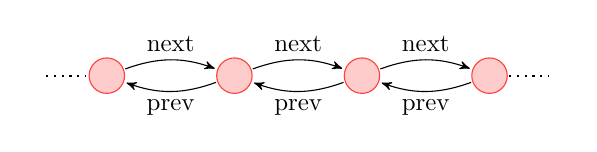
\begin{tikzpicture}[node distance=1.8cm,>=stealth',bend angle=45,auto
,shorten >=1pt,shorten <=0.5pt,thin,->
,scale=0.9, every node/.style={transform shape}
]

  \tikzstyle{cell}=[circle,thick,draw=black,minimum size=5mm]
  \tikzstyle{red cell}=[circle,draw=red!75,fill=red!20,minimum size=5mm]

%  \tikzstyle{every label}=[red]

  \begin{scope}%[mylabel/.style={scale=0.8}]%[every label/.style={scale=0.8}]
	
    % First net
    \node (c0) {};
    \node [red cell,right of=c0,node distance=1cm] (c1) {};
    \node [red cell,right of=c1] (c2) {};
    \node [red cell,right of=c2] (c3) {};
    \node [red cell,right of=c3] (c4) {};
    \node [right of=c4,node distance=1cm](c5) {};

	\path 
         (c0) edge [dotted,thick,-] (c1)

         (c1) edge [bend left=20] node  {\figtext{next}} (c2)
         (c2) edge [bend left=20] node  {\figtext{prev}} (c1)

         (c2) edge [bend left=20] node  {\figtext{next}} (c3)
         (c3) edge [bend left=20] node  {\figtext{prev}} (c2)

         (c3) edge [bend left=20] node  {\figtext{next}} (c4)
         (c4) edge [bend left=20] node  {\figtext{prev}} (c3)

         (c4) edge [dotted,thick,-] (c5)

    ;
  \end{scope}

\end{tikzpicture}

  \end{center}
  \caption{A part of a DLL}
  \label{fig:decomp_c}
  \end{subfigure}

  \noindent
  \begin{subfigure}[b]{0.6\linewidth}
  \begin{center}
    
%%%%%%%%%%%%%%%%%%%%%%%%%%%%%%%%%%%%%%%%%%%%%%%%%%%%%%%%%%%%%%%%%%%%%%%
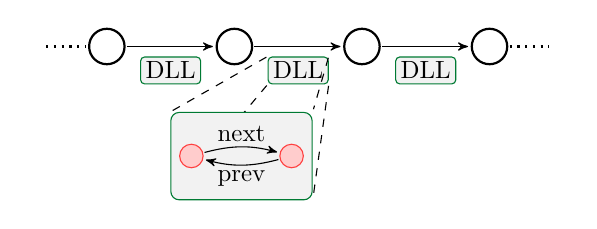
\begin{tikzpicture}[node distance=1.8cm,>=stealth',bend angle=45,auto
,shorten >=1pt,shorten <=0.5pt,thin,->
,scale=0.9, every node/.style={transform shape}
]

  \tikzstyle{cell}=[circle,thick,draw=black,minimum size=5mm]
  \tikzstyle{red cell}=[circle,draw=red!75,fill=red!20,minimum size=3mm]
  \tikzstyle{box}=[draw=green!60!black!80!blue,fill=black!5,swap,yshift=-4pt, inner sep=2pt,rounded corners=1.5pt]

%  \tikzstyle{every label}=[red]

  \begin{scope}%[mylabel/.style={scale=0.8}]%[every label/.style={scale=0.8}]
	
    % First net
    \node (c0) {};
    \node [cell,right of=c0,node distance=1cm] (c1) {};
    \node [cell,right of=c1] (c2) {};
    \node [cell,right of=c2] (c3) {};
    \node [cell,right of=c3] (c4) {};
    \node [right of=c4,node distance=1cm](c5) {};


	\begin{pgfonlayer}{background}
	\path 
         (c0) edge [dotted,thick,-] (c1)
         (c1) edge node [box] (b1) {\figtext{DLL}} (c2)
         (c2) edge node [box] (b2) {\figtext{DLL}} (c3)
         (c3) edge node [box] (b3) {\figtext{DLL}} (c4)
         (c4) edge [dotted,thick,-] (c5)
    ;
	\end{pgfonlayer}

    \node [red cell, below left of=b2,node distance=1cm,xshift=-0.8cm,yshift=-0.5cm] (c6) {};
    \node [red cell, below right of=b2, node distance=1cm,xshift=-0.8cm,yshift=-0.5cm] (c7) {};

    \path
         (c6) edge [bend left=15] node [inner sep=2pt] (bla1) {\figtext{next}} (c7)
         (c7) edge [bend left=15] node [inner sep=2pt] (bla2) {\figtext{prev}} (c6)
    ;

	\begin{pgfonlayer}{background}
	\node [fit=(c6) (c7) (bla1) (bla2),rounded corners=3pt,inner sep=3pt] (big) {};

    \path
      (b2.north west) edge [dashed,-] (big.north west)
      (b2.north east) edge [dashed,-] (big.north east)
      (b2.south west) edge [dashed,-] (big.south west)
      (b2.south east) edge [dashed,-] (big.south east)
    ;

	\node [draw=green!60!black!80!blue,fill=black!5,fit=(c6) (c7) (bla1) (bla2),rounded corners=3pt,inner sep=3pt] {};
	\end{pgfonlayer}

  \end{scope}

\end{tikzpicture}

  \end{center}
  \caption{A hierarchical encoding of the DLL}
  \label{fig:decomp_d}
  \end{subfigure}

  % \begin{tabular}{c}
  %   \begin{minipage}{0.6\textwidth}\begin{center}
%%%%%%%%%%%%%%%%%%%%%%%%%%%%%%%%%%%%%%%%%%%%%%%%%%%%%%%%%%%%%%%%%%%%%%%
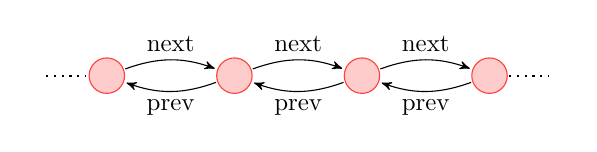
\begin{tikzpicture}[node distance=1.8cm,>=stealth',bend angle=45,auto
,shorten >=1pt,shorten <=0.5pt,thin,->
,scale=0.9, every node/.style={transform shape}
]

  \tikzstyle{cell}=[circle,thick,draw=black,minimum size=5mm]
  \tikzstyle{red cell}=[circle,draw=red!75,fill=red!20,minimum size=5mm]

%  \tikzstyle{every label}=[red]

  \begin{scope}%[mylabel/.style={scale=0.8}]%[every label/.style={scale=0.8}]
	
    % First net
    \node (c0) {};
    \node [red cell,right of=c0,node distance=1cm] (c1) {};
    \node [red cell,right of=c1] (c2) {};
    \node [red cell,right of=c2] (c3) {};
    \node [red cell,right of=c3] (c4) {};
    \node [right of=c4,node distance=1cm](c5) {};

	\path 
         (c0) edge [dotted,thick,-] (c1)

         (c1) edge [bend left=20] node  {\figtext{next}} (c2)
         (c2) edge [bend left=20] node  {\figtext{prev}} (c1)

         (c2) edge [bend left=20] node  {\figtext{next}} (c3)
         (c3) edge [bend left=20] node  {\figtext{prev}} (c2)

         (c3) edge [bend left=20] node  {\figtext{next}} (c4)
         (c4) edge [bend left=20] node  {\figtext{prev}} (c3)

         (c4) edge [dotted,thick,-] (c5)

    ;
  \end{scope}

\end{tikzpicture}
\end{center}\end{minipage}\\
  %   (a)\\
  %   \begin{minipage}{0.6\textwidth}\begin{center}
%%%%%%%%%%%%%%%%%%%%%%%%%%%%%%%%%%%%%%%%%%%%%%%%%%%%%%%%%%%%%%%%%%%%%%%
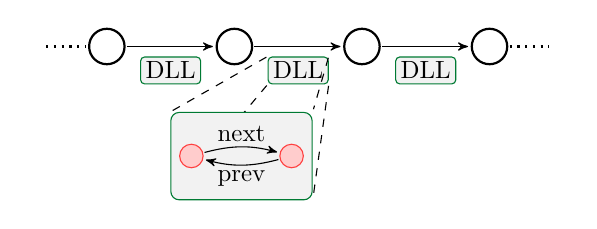
\begin{tikzpicture}[node distance=1.8cm,>=stealth',bend angle=45,auto
,shorten >=1pt,shorten <=0.5pt,thin,->
,scale=0.9, every node/.style={transform shape}
]

  \tikzstyle{cell}=[circle,thick,draw=black,minimum size=5mm]
  \tikzstyle{red cell}=[circle,draw=red!75,fill=red!20,minimum size=3mm]
  \tikzstyle{box}=[draw=green!60!black!80!blue,fill=black!5,swap,yshift=-4pt, inner sep=2pt,rounded corners=1.5pt]

%  \tikzstyle{every label}=[red]

  \begin{scope}%[mylabel/.style={scale=0.8}]%[every label/.style={scale=0.8}]
	
    % First net
    \node (c0) {};
    \node [cell,right of=c0,node distance=1cm] (c1) {};
    \node [cell,right of=c1] (c2) {};
    \node [cell,right of=c2] (c3) {};
    \node [cell,right of=c3] (c4) {};
    \node [right of=c4,node distance=1cm](c5) {};


	\begin{pgfonlayer}{background}
	\path 
         (c0) edge [dotted,thick,-] (c1)
         (c1) edge node [box] (b1) {\figtext{DLL}} (c2)
         (c2) edge node [box] (b2) {\figtext{DLL}} (c3)
         (c3) edge node [box] (b3) {\figtext{DLL}} (c4)
         (c4) edge [dotted,thick,-] (c5)
    ;
	\end{pgfonlayer}

    \node [red cell, below left of=b2,node distance=1cm,xshift=-0.8cm,yshift=-0.5cm] (c6) {};
    \node [red cell, below right of=b2, node distance=1cm,xshift=-0.8cm,yshift=-0.5cm] (c7) {};

    \path
         (c6) edge [bend left=15] node [inner sep=2pt] (bla1) {\figtext{next}} (c7)
         (c7) edge [bend left=15] node [inner sep=2pt] (bla2) {\figtext{prev}} (c6)
    ;

	\begin{pgfonlayer}{background}
	\node [fit=(c6) (c7) (bla1) (bla2),rounded corners=3pt,inner sep=3pt] (big) {};

    \path
      (b2.north west) edge [dashed,-] (big.north west)
      (b2.north east) edge [dashed,-] (big.north east)
      (b2.south west) edge [dashed,-] (big.south west)
      (b2.south east) edge [dashed,-] (big.south east)
    ;

	\node [draw=green!60!black!80!blue,fill=black!5,fit=(c6) (c7) (bla1) (bla2),rounded corners=3pt,inner sep=3pt] {};
	\end{pgfonlayer}

  \end{scope}

\end{tikzpicture}
\end{center}\end{minipage}\\
  %   (b)
  % \end{tabular}

  % \caption{(a) A part of a DLL, (b) a hierarchical encoding of the DLL.}
  \caption{Encoding of a~DLL using boxes}

  \label{figDecomposition2}

\end{center}
\end{figure}


The described encoding allows one to represent sets of heaps with a~bounded
number of cut-points. Many common dynamic data structures,
however, have an \emph{unbounded number of
cut-points}. Indeed, for instance, in doubly-linked lists (DLLs), every node is
a cut-point. We solve the problem of an unbounded number of cut-points by
representing heaps in a \emph{hierarchical
way}. In particular, we collect sets of repeated subgraphs (called
\emph{components}) containing cut-points into the so-called \emph{boxes}. Every
occurrence of such components can then be replaced by a single edge labelled by
the appropriate box. To specify how a subgraph enclosed within a~box is
connected to the rest of the graph, the subgraph is equipped with the so-called
input and output ports. The source vertex of a box then matches the input port
of the subgraph, and the target vertex of the edge matches the output
port.\footnote{Later on, the term \emph{input port} will be used to refer to the nodes
pointed to by program variables too since these nodes play a similar role as the
inputs of components.} In this way, a set of heap graphs with an unbounded
number of cut-points can be transformed into a set of \emph{hierarchical heap
graphs} with a~bounded number of cut-points at each level of the hierarchy.
Figs.~\ref{fig:decomp_c} and~\ref{fig:decomp_d} illustrate how this approach can
reduce the representation of DLLs into singly-linked lists (with a~DLL segment
used as a~kind of a~meta-selector). 


\begin{figure}[t]
\begin{center}

  \begin{subfigure}[b]{0.36\linewidth}
  \begin{center}
  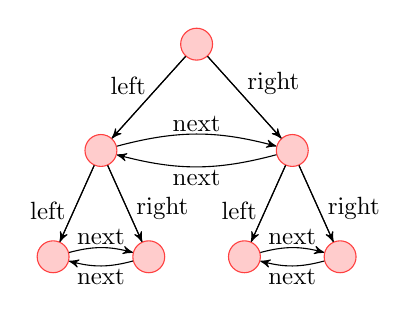
\begin{tikzpicture}[level distance=15mm, level/.style={sibling distance=27mm/#1}, node distance=1cm,>=stealth',bend angle=45,scale=0.9,auto
, every node/.style={transform shape}
]

  \tikzstyle{cell}=[circle,thick,draw=black,minimum size=4.5mm]
  \tikzstyle{red cell}=[circle,draw=red!75,fill=red!20,minimum size=4.5mm]
  \tikzstyle{data}=[rectangle,thick,draw=black!75,
  			  fill=black!20,minimum size=3mm]

  \tikzstyle{every label}=[red]

    \node [red cell] (c1)                             {}
      child{ node [red cell] (c11)               {}
        child{ node [red cell] (c111)          {} }
        child{ node [red cell] (c112)          {} }
      }
      child{ node [red cell] (c12)              {}
        child{ node [red cell] (c121)          {} }
        child{ node [red cell] (c122)          {} }
      };

    \path (c1)  edge [swap,->,inner sep=1pt]  node  {\figtext{left}} (c11);
    \path (c1)  edge [->,inner sep=1pt]  node  {\figtext{right}} (c12);

    \path (c11)  edge [bend left=15,->,inner sep=1pt]  node  {\figtext{next}} (c12);
    \path (c12)  edge [bend left=15,->,inner sep=1pt]  node  {\figtext{next}} (c11);

    \path (c11)  edge [swap,->,inner sep=1pt]  node [near end] {\figtext{left}} (c111);
    \path (c11)  edge [->,inner sep=1pt]  node [near end] {\figtext{right}} (c112);

    \path (c111)  edge [bend left=15,->,inner sep=1pt]  node  {\figtext{next}} (c112);
    \path (c112)  edge [bend left=15,->,inner sep=1pt]  node  {\figtext{next}} (c111);

    \path (c12)  edge [swap,->,inner sep=1pt]  node [near end] {\figtext{left}} (c121);
    \path (c12)  edge [->,inner sep=1pt]  node [near end] {\figtext{right}} (c122);

    \path (c121)  edge [bend left=15,->,inner sep=1pt]  node  {\figtext{next}} (c122);
    \path (c122)  edge [bend left=15,->,inner sep=1pt]  node  {\figtext{next}} (c121);

\end{tikzpicture}


  \end{center}
  \caption{A tree with linked sibling nodes}
  \label{fig:hyper_a}
  \end{subfigure}
  \hfill
  \begin{subfigure}[b]{0.24\linewidth}
  \begin{center}
  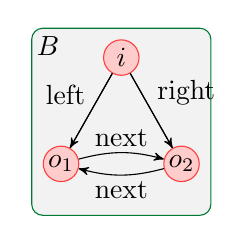
\begin{tikzpicture}[level distance=15mm, level/.style={sibling distance=17mm/#1}, node distance=1cm,>=stealth',bend angle=45,scale=0.9,auto
%,scale=2
%,every node/.style={transform shape}
]

  \tikzstyle{cell}=[circle,thick,draw=black,minimum size=4.5mm]
  \tikzstyle{red cell}=[circle,draw=red!75,fill=red!20,minimum size=4.5mm]
  \tikzstyle{data}=[rectangle,thick,draw=black!75,
  			  fill=black!20,minimum size=3mm]

  \tikzstyle{every label}=[red]

    \node [red cell,inner sep=0pt] (c1)                             {$i$}
      child{ node [red cell,inner sep=0pt] (c11)               {$o_1$} }
      child{ node [red cell,inner sep=0pt] (c12)              {$o_2$} };

    \node [left of=c1,yshift=4pt,xshift=2pt] {$B$};

    \path (c1)  edge [swap,->] coordinate [midway] (f1)  node [inner sep=2pt] (bla1)  {\figtext{left}} (c11);
    \path (c1)  edge [->]   coordinate [midway] (f2)  node [inner sep=2pt] (bla2) {\figtext{right}} (c12);

    \path (c11)  edge [bend left=15,->]  node [inner sep=2pt] {\figtext{next}} (c12);
    \path (c12)  edge [bend left=15,->]  node [inner sep=2pt] (bla3) {\figtext{next}} (c11);
	
%	\draw [black] (f1) to[out=-30,in=-150] (f2) node [midway,anchor=north,inner sep=8pt] {\figtext{B}};

	\begin{pgfonlayer}{background}
	\node [draw=green!60!black!80!blue,fill=black!5,fit=(c1) (c11) (c12) (bla3),rounded corners=4pt,inner sep=4pt] {};
	\end{pgfonlayer}
	

\end{tikzpicture}


  \vspace{-2mm}
  \end{center}
  \caption{A pattern that repeats in the structure and that is linked in such a
    way that all nodes in the structure are cut-points}
  \label{fig:hyper_b}
  \end{subfigure}
  \hfill
  \begin{subfigure}[b]{0.35\linewidth}
  \begin{center}
  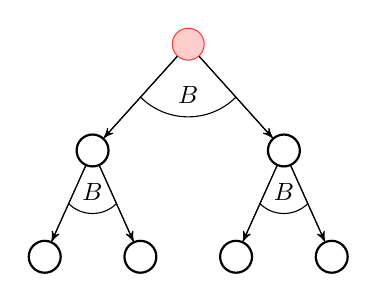
\begin{tikzpicture}[level distance=15mm, level/.style={sibling distance=27mm/#1}, node distance=1cm,>=stealth',bend angle=45,scale=0.9,auto
, every node/.style={transform shape}
]

  \tikzstyle{cell}=[circle,thick,draw=black,minimum size=4.5mm]
  \tikzstyle{red cell}=[circle,draw=red!75,fill=red!20,minimum size=4.5mm]

  \tikzstyle{every label}=[red]

    \node [red cell] (c1)                             {}
      child{ node [cell] (c11)               {}
        child{ node [cell] (c111)          {} }
        child{ node [cell] (c112)          {} }
      }
      child{ node [cell] (c12)              {}
        child{ node [cell] (c121)          {} }
        child{ node [cell] (c122)          {} }
      };

%    \path (c1)  edge [swap,->] coordinate [midway] (f1)  node  {\figtext{left}} (c11);
%    \path (c1)  edge [->]  coordinate [midway] (f2) node  {\figtext{right}} (c12);
    \path (c1)  edge [swap,->] coordinate [midway] (f1)  node  {} (c11);
    \path (c1)  edge [->]  coordinate [midway] (f2) node  {} (c12);

	\path [draw,black] (f1) to[out=-45,in=-135] node [midway,inner sep=5pt] {$B$} (f2);

%    \path (c11)  edge [bend left=9,->]  node  {\figtext{next}} (c12);
%    \path (c12)  edge [bend left=9,->]  node  {\figtext{next}} (c11);

%    \path (c11)  edge [swap,->]  coordinate [midway] (f3) node [yshift=-2mm]  {\figtext{left}} (c111);
%    \path (c11)  edge [->]  coordinate [midway] (f4) node [yshift=-2mm]  {\figtext{right}} (c112);
    \path (c11)  edge [swap,->]  coordinate [midway] (f3) node [yshift=-2mm]  {} (c111);
    \path (c11)  edge [->]  coordinate [midway] (f4) node [yshift=-2mm]  {} (c112);

	\draw [black] (f3) to[out=-45,in=-135] node [midway,inner sep=5pt] {$B$} (f4);

%    \path (c111)  edge [bend left=9,->]  node  {\figtext{next}} (c112);
%    \path (c112)  edge [bend left=9,->]  node  {\figtext{next}} (c111);

%    \path (c12)  edge [swap,->]  coordinate [midway] (f5) node [yshift=-2mm]  {\figtext{left}} (c121);
%    \path (c12)  edge [->] coordinate [midway] (f6) node [yshift=-2mm]  {\figtext{right}} (c122);
    \path (c12)  edge [swap,->]  coordinate [midway] (f5) node [yshift=-2mm]  {} (c121);
    \path (c12)  edge [->] coordinate [midway] (f6) node [yshift=-2mm]  {} (c122);

	\draw [black] (f5) to[out=-45,in=-135] node [midway,inner sep=5pt] {$B$} (f6);

%    \path (c121)  edge [bend left=9,->]  node  {\figtext{next}} (c122);
%    \path (c122)  edge [bend left=9,->]  node  {\figtext{next}} (c121);

\end{tikzpicture}


  \end{center}
  \caption{The tree with linked sibling nodes represented using
    hyperedges labelled by the box $B$}
  \label{fig:hyper_c}
  \end{subfigure}

  % \begin{tabular}{c@{}c@{}c}
  %   \begin{minipage}[t]{0.36\textwidth}\begin{center}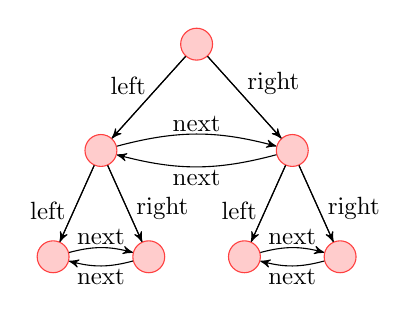
\begin{tikzpicture}[level distance=15mm, level/.style={sibling distance=27mm/#1}, node distance=1cm,>=stealth',bend angle=45,scale=0.9,auto
, every node/.style={transform shape}
]

  \tikzstyle{cell}=[circle,thick,draw=black,minimum size=4.5mm]
  \tikzstyle{red cell}=[circle,draw=red!75,fill=red!20,minimum size=4.5mm]
  \tikzstyle{data}=[rectangle,thick,draw=black!75,
  			  fill=black!20,minimum size=3mm]

  \tikzstyle{every label}=[red]

    \node [red cell] (c1)                             {}
      child{ node [red cell] (c11)               {}
        child{ node [red cell] (c111)          {} }
        child{ node [red cell] (c112)          {} }
      }
      child{ node [red cell] (c12)              {}
        child{ node [red cell] (c121)          {} }
        child{ node [red cell] (c122)          {} }
      };

    \path (c1)  edge [swap,->,inner sep=1pt]  node  {\figtext{left}} (c11);
    \path (c1)  edge [->,inner sep=1pt]  node  {\figtext{right}} (c12);

    \path (c11)  edge [bend left=15,->,inner sep=1pt]  node  {\figtext{next}} (c12);
    \path (c12)  edge [bend left=15,->,inner sep=1pt]  node  {\figtext{next}} (c11);

    \path (c11)  edge [swap,->,inner sep=1pt]  node [near end] {\figtext{left}} (c111);
    \path (c11)  edge [->,inner sep=1pt]  node [near end] {\figtext{right}} (c112);

    \path (c111)  edge [bend left=15,->,inner sep=1pt]  node  {\figtext{next}} (c112);
    \path (c112)  edge [bend left=15,->,inner sep=1pt]  node  {\figtext{next}} (c111);

    \path (c12)  edge [swap,->,inner sep=1pt]  node [near end] {\figtext{left}} (c121);
    \path (c12)  edge [->,inner sep=1pt]  node [near end] {\figtext{right}} (c122);

    \path (c121)  edge [bend left=15,->,inner sep=1pt]  node  {\figtext{next}} (c122);
    \path (c122)  edge [bend left=15,->,inner sep=1pt]  node  {\figtext{next}} (c121);

\end{tikzpicture}

\end{center}\end{minipage}&
  %   \begin{minipage}[t]{0.27\textwidth}\begin{center}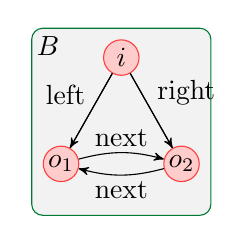
\begin{tikzpicture}[level distance=15mm, level/.style={sibling distance=17mm/#1}, node distance=1cm,>=stealth',bend angle=45,scale=0.9,auto
%,scale=2
%,every node/.style={transform shape}
]

  \tikzstyle{cell}=[circle,thick,draw=black,minimum size=4.5mm]
  \tikzstyle{red cell}=[circle,draw=red!75,fill=red!20,minimum size=4.5mm]
  \tikzstyle{data}=[rectangle,thick,draw=black!75,
  			  fill=black!20,minimum size=3mm]

  \tikzstyle{every label}=[red]

    \node [red cell,inner sep=0pt] (c1)                             {$i$}
      child{ node [red cell,inner sep=0pt] (c11)               {$o_1$} }
      child{ node [red cell,inner sep=0pt] (c12)              {$o_2$} };

    \node [left of=c1,yshift=4pt,xshift=2pt] {$B$};

    \path (c1)  edge [swap,->] coordinate [midway] (f1)  node [inner sep=2pt] (bla1)  {\figtext{left}} (c11);
    \path (c1)  edge [->]   coordinate [midway] (f2)  node [inner sep=2pt] (bla2) {\figtext{right}} (c12);

    \path (c11)  edge [bend left=15,->]  node [inner sep=2pt] {\figtext{next}} (c12);
    \path (c12)  edge [bend left=15,->]  node [inner sep=2pt] (bla3) {\figtext{next}} (c11);
	
%	\draw [black] (f1) to[out=-30,in=-150] (f2) node [midway,anchor=north,inner sep=8pt] {\figtext{B}};

	\begin{pgfonlayer}{background}
	\node [draw=green!60!black!80!blue,fill=black!5,fit=(c1) (c11) (c12) (bla3),rounded corners=4pt,inner sep=4pt] {};
	\end{pgfonlayer}
	

\end{tikzpicture}

\end{center}\end{minipage}&
  %   \begin{minipage}[t]{0.34\textwidth}\begin{center}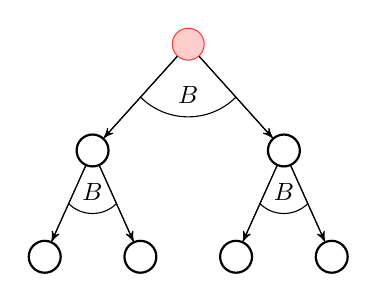
\begin{tikzpicture}[level distance=15mm, level/.style={sibling distance=27mm/#1}, node distance=1cm,>=stealth',bend angle=45,scale=0.9,auto
, every node/.style={transform shape}
]

  \tikzstyle{cell}=[circle,thick,draw=black,minimum size=4.5mm]
  \tikzstyle{red cell}=[circle,draw=red!75,fill=red!20,minimum size=4.5mm]

  \tikzstyle{every label}=[red]

    \node [red cell] (c1)                             {}
      child{ node [cell] (c11)               {}
        child{ node [cell] (c111)          {} }
        child{ node [cell] (c112)          {} }
      }
      child{ node [cell] (c12)              {}
        child{ node [cell] (c121)          {} }
        child{ node [cell] (c122)          {} }
      };

%    \path (c1)  edge [swap,->] coordinate [midway] (f1)  node  {\figtext{left}} (c11);
%    \path (c1)  edge [->]  coordinate [midway] (f2) node  {\figtext{right}} (c12);
    \path (c1)  edge [swap,->] coordinate [midway] (f1)  node  {} (c11);
    \path (c1)  edge [->]  coordinate [midway] (f2) node  {} (c12);

	\path [draw,black] (f1) to[out=-45,in=-135] node [midway,inner sep=5pt] {$B$} (f2);

%    \path (c11)  edge [bend left=9,->]  node  {\figtext{next}} (c12);
%    \path (c12)  edge [bend left=9,->]  node  {\figtext{next}} (c11);

%    \path (c11)  edge [swap,->]  coordinate [midway] (f3) node [yshift=-2mm]  {\figtext{left}} (c111);
%    \path (c11)  edge [->]  coordinate [midway] (f4) node [yshift=-2mm]  {\figtext{right}} (c112);
    \path (c11)  edge [swap,->]  coordinate [midway] (f3) node [yshift=-2mm]  {} (c111);
    \path (c11)  edge [->]  coordinate [midway] (f4) node [yshift=-2mm]  {} (c112);

	\draw [black] (f3) to[out=-45,in=-135] node [midway,inner sep=5pt] {$B$} (f4);

%    \path (c111)  edge [bend left=9,->]  node  {\figtext{next}} (c112);
%    \path (c112)  edge [bend left=9,->]  node  {\figtext{next}} (c111);

%    \path (c12)  edge [swap,->]  coordinate [midway] (f5) node [yshift=-2mm]  {\figtext{left}} (c121);
%    \path (c12)  edge [->] coordinate [midway] (f6) node [yshift=-2mm]  {\figtext{right}} (c122);
    \path (c12)  edge [swap,->]  coordinate [midway] (f5) node [yshift=-2mm]  {} (c121);
    \path (c12)  edge [->] coordinate [midway] (f6) node [yshift=-2mm]  {} (c122);

	\draw [black] (f5) to[out=-45,in=-135] node [midway,inner sep=5pt] {$B$} (f6);

%    \path (c121)  edge [bend left=9,->]  node  {\figtext{next}} (c122);
%    \path (c122)  edge [bend left=9,->]  node  {\figtext{next}} (c121);

\end{tikzpicture}

\end{center}\end{minipage}\\
  %   (a) & (b) & (c)
  % \end{tabular}

  \caption{An example of a~data structure where boxes with multiple output ports
  are necessary}
  % \caption{(a) A tree with linked sibling nodes, (b) a pattern that repeats in
  % the structure and that is linked in such a way that all nodes in the structure
  % are cut-points, (c) the tree with linked brother nodes represented using
  % hyperedges labelled by the box $B$.}

  \label{figLinkedBrothers}

\end{center}
\end{figure}

In general, we allow a box to have more than one output port. Boxes with
multiple output ports, however, reduce heap graphs not to graphs but rather
\emph{hypergraphs} with \emph{hyperedges} having a single source node, but
multiple target nodes. This situation is illustrated on a simple example shown
in Fig.~\ref{figLinkedBrothers}. The tree with linked siblings from
Fig.~\ref{fig:hyper_a} is turned into a hypergraph with binary
hyperedges shown in Fig.~\ref{fig:hyper_c} using the box~$B$ from
Fig.~\ref{fig:hyper_b}. The subgraph encoded by the box $B$ can be
connected to its surroundings via its input port~$i$ and \emph{two} output
ports~$o_1$ and~$o_2$.
Therefore, the hypergraph from Fig.~\ref{fig:hyper_c}
encodes one level of the tree by a~hyperedge with one source and \emph{two}
target nodes.
%
A formalisation using hypergraphs and hyperedges was used in \cite{habermehl:forest}.
Here, in order to simplify the formal development, we will stay with ordinary graphs, 
in which a hyperedge is represented by a~set of ordinary edges (which always
need to occur together) from a single source to several targets.

Sets of heap graphs corresponding either to the  top level of the
representation or to boxes of different levels can then be decomposed into
tree components and represented using \emph{hierarchical FAs}, whose
alphabets can contain nested FAs.
Intuitively, FAs appearing in the alphabet of some higher-level FA play a~role
in some sense similar to that of inductive predicates in  separation
logic.\footnote{For
instance, we use a nested FA to encode a DLL segment of length 1.  In separation
logic, the corresponding inductive predicate would represent segments of length
1 or more. In our approach, the repetition of the segment is encoded in the
structure of the top-level~FA.} We restrict ourselves to automata whose nesting forms
a~finite and strict hierarchy (i.e., there is no circular use of the automata in
their alphabets). 
This is obviously different from separation logic, where recursive inductive predicates are standard.
This kind of recursion is in forest automata represented through cycles of tree automata transitions.


%\annot[lh]{removed talking about entailment}
%The question of deciding inclusion on sets of heaps represented by hierarchical
%FA remains open. However, we propose a \emph{canonical decomposition of
%hierarchical hypergraphs} allowing inclusion to be decided for sets of heap
%hypergraphs represented by FA provided that the nested FA labelling hyperedges
%are taken as atomic alphabet symbols. Note that this decomposition is by far not
%the same as for non-hierarchical heap graphs due to a need to deal with nodes
%that are not reachable on the top level, but are reachable through edges hidden
%in some boxes. This result allows us to safely approximate inclusion checking on
%hierarchically represented heaps, which appears to work quite well in practice. 





%%%%%%%%%%%%%%%%%%%%%%%%%%%%%%%%%%%%%%%%%%%%%%%%%%%%%%%%%%%%%%%%%%%%%
\section{Forest Automata and Heaps}
%%%%%%%%%%%%%%%%%%%%%%%%%%%%%%%%%%%%%%%%%%%%%%%%%%%%%%%%%%%%%%%%%%%%%

% \td{OL: talk only about heaps}

We consider sequential non-recursive C programs operating on a set of pointer
variables and the heap using standard statements and control flow constructs.
%Variables are either \emph{data variables} or \emph{pointer variables}.
Heap cells contain zero or several pointer or data fields.
%(our framework and implementation extends easily to several data fields).
% \comment[mh]{Why do you speak about commands here?}
%The supported statements include allocation and deallocation of heap memory,
%tests between data variables or fields of heap cells, as well as assignments
%between data variables, pointer variables, or fields of heap cells.

%\begin{figure}
%% \vspace{10mm}
%% \hspace{-4mm}
%\begin{center}
%\begin{tikzpicture}[%
%  codeblock/.style={text width=0.4\linewidth,rounded corners,inner xsep=12pt,inner ysep=0pt,below right,draw=gray!3!white},%
%  property/.style={rounded corners=1pt,inner xsep=1mm,draw=black!50,fill=white,double}%
%  ]
%  \node[codeblock] (code) {\small\VerbatimInput{code.txt}};
%\end{tikzpicture}%
%\end{center}
%\vspace*{-1mm}
%\caption{A function which inserts a~new node into a BST and returns a~pointer to
%its root node.}
%\label{fig:bst-code}
%\end{figure}
%
%Fig.~\ref{fig:bst-code} shows an example of a C function inserting a new node
%into a~BST (recall that in BSTs, the data value in a node is larger than all
%the values of its left subtree and smaller than all the values of its right
%subtree). Variable $\code{x}$ descends the BST to find the position at which
%the node $\code{newNode}$ with a new data value $\code{d}$ should be inserted.

Configurations of the considered programs consist of
memory-allocated data and an assignment of variables.
\emph{Heap memory} can be viewed as a~(directed) graph whose nodes correspond
to allocated memory cells.
Every node contains a~set of named pointer and data fields.
Each pointer field points to another node (we model the
$\code{NULL}$ address and undefined locations as special memory nodes pointed by variables
$\code{NULL}$ and $\code{undef}$, respectively), and the same holds for pointer variables of the program.
Data fields of memory nodes hold a~data value.
We use the term \emph{selector} to talk both about pointer and data fields.
For simplification, we model data variables as pointer variables pointing to
allocated nodes that contain a single data field with the value of the
variable, and therefore consider only pointer
variables hereafter.
%In our terminology, a~\emph{heap} consists of a~heap memory and mapping of
%(pointer) variables to memory nodes.

%% We represent heap memory as a~composition of trees as follows. We first identify the
%% \emph{cut-points} of the heap, i.e., nodes that are either referenced by a
%% pointer variable or by several selectors. We then split the heap into
%% (cut-point-free) tree
%% components such that each cut-point becomes the root of a tree component. To
%% represent the interconnection of tree components, we introduce a set of
%% \emph{root references}, one for each tree component. After decomposition of the
%% heap, selectors and variables that point to cut-points in the heap are redirected to
%% point to the corresponding root references. Such a tuple of tree components
%% (together with the mapping of variables) is called a~\emph{forest}.
%% The decomposition of a~heap into tree components can be
%% performed canonically as described at the end of Section~\ref{sec:fa}.

We represent heap memory by partitioning it into a~tuple of trees, the
so-called \emph{forest}.
The leaves of the trees contain information about roots of which trees they should be merged with to recover the original heap. 
Our \emph{forest automata} symbolic representations of sets of heaps is based
on representing sets of forests using tuples of tree automata.
%

% \td{OL: keep the example? START}
% \td{OL: maybe substitute with Fig.~\ref{fig:forest_rep}?}
% Fig.~\ref{fig:bst-graph}(a) shows a possible heap of the program in
% Fig.~\ref{fig:bst-code}. Nodes are shown as circles, labeled by their data
% values. Selectors are shown as edges. Each selector points either to a~node or
% to $\nullconst$ (denoting \texttt{NULL}). Some nodes are labeled by a~pointer
% variable that points to them. The node with data value $15$ is a cut-point since
% it is referenced by variable $\code{x}$. Fig.~\ref{fig:bst-graph}(b) shows a
% tree decomposition of the graph into two trees, one rooted at the node
% referenced by $\code{root}$, and the other rooted at the node pointed by
% $\code{x}$. The $\code{right}$ selector of the root node in the first tree
% points to root reference $\rr{2}$ ($\rr{i}$ denotes a reference to the $i$-th
% tree $\tree_i$) to indicate that in the graph, it points to the corresponding
% cut-point.
% \td{OL: keep the example? END}

%%% kicked out for the submission
%%% Fig.~\ref{fig:forest_rep_graph} shows an example of a~(data-free) heap;
%%% nodes are shown as circles, selectors are shown as edges.
%%% Each selector points either to a~node or to $\nullconst$ (denoting
%%% an edge to the \texttt{NULL} node).
%%% Some nodes are labeled by a~pointer variable that points to them.
%%% The nodes labelled with 1 and 3 are cut-points because they are pointed by
%%% variables (\texttt{x} and \texttt{y} respectively) and the node labelled with 2
%%% is a cut-point because it has two incoming edges.
%%% Fig.~\ref{fig:forest_rep_forest} shows a~forest representation of the heap from
%%% Fig.~\ref{fig:forest_rep_graph}.

%Let us now formalize these ideas.
%%% In the following, we use $f: A \partialto B$ to denote a partial function from
%%% \annot[lh]{is this used?}
%%% $A$ to $B$ (also
%%% viewed as a~total function $f: A \to (B \cup \set{\bot})$, assuming that $\bot
%%% \not\in B$).
%%% We also assume a bounded data domain $\dset$. 

% \begin{figure}[t]
%   \begin{minipage}[b]{5.6cm}
%     \centering
%     \vspace{-2mm}
%     \input{figs/bst_graph.tex}
%
%     \vspace{-1mm}
%     \small (a) A~graph.
%   \end{minipage}
%   \begin{minipage}[b]{6.8cm}
%     \begin{minipage}[t]{2.8cm}
%       \input{figs/bst_forest.tex}
%     \end{minipage}
%     \hspace{-0.0cm}
%     \begin{minipage}[t]{1.5cm}
%       \input{figs/bst_tree.tex}
%     \end{minipage}
%
%     \vspace{-1mm}
%     \centering
%    \small (b) A forest decomposition.
%   \end{minipage}
%   \vspace{-1mm}
%   \caption{Decomposition of a graph into trees.}
% \label{fig:bst-graph}
% \end{figure}

%% kicked out for the first submission
%% \begin{figure}[t]
%%   \begin{subfigure}[b]{0.48\textwidth}
%%   \centering
%%   \input{figs/fa-tree-decomp-graph.tikz}
%%   \caption{A~heap}
%%   \label{fig:forest_rep_graph}
%%   \end{subfigure}
%%   \hfill
%%   \begin{subfigure}[b]{0.48\textwidth}
%%   \centering
%%   \input{figs/fa-tree-decomp-forest.tikz}
%%   \caption{Its forest representation}
%%   \label{fig:forest_rep_forest}
%%   \end{subfigure}
%% \caption{A~heap and its forest representation.  For simplification, edges to
%% the dedicated $\nil$ node are represented using $\nullconst$ (we omit the
%% node from the graphical representation).}
%% \label{fig:forest_rep}
%% \end{figure}

%\bigskip
%\lukas{throw away $\leaflab$ completely? We can assume that $\abcd$ does not intersect with $\{\bar i\mid i\in\nat\}$ and use trees over $\abcd\cup\{\bar 1\,\ldots\bar n\}$ It looks like the only instantiation of $\leaflab$ is the $\{\bar 1,\ldots,\bar n\}$ anyway.}

%-------------------------------------------------------------------------------
% \subsection{Graphs and Heaps}\label{sec:label}
\subsection*{Graphs and Heaps}
%-------------------------------------------------------------------------------


Let $\abcd$ be a finite set of \emph{selectors} and $\leaflab$ be a~finite set
of \emph{references} such that $\leaflab \cap \dset = \emptyset$.
A~\emph{graph}~$\graph$ over $\tuple{\abcd,\leaflab}$ is
% A~\emph{graph}~$\graph$ over $\abcd$ is
a tuple $\tuple{\nodesof{\graph},\selmapof{\graph}}$ where
$\nodesof{\graph}$ is a~finite set  of \emph{nodes} and $\selmapof{\graph}: \abcd \to (\nodesof{\graph}
\partialto (\nodesof{\graph}\cup \leaflab \cup \dset))$ maps each selector $a \in \abcd$
to a~partial mapping $\selmapof{\graph}(a)$ from nodes to nodes, references, or
data values.
%
References and data values are treated as special terminal
nodes that are not in the set of regular nodes, i.e., $V_g \cap (\leaflab \cup
\dset) = \emptyset$.
%
For a~graph~$\graph$, we use $\nodesof \graph$ to denote the nodes of~$\graph$,
and for a selector $a \in \abcd$, we
use $\selof{\graph}$ to denote the mapping $\selmapof{\graph}(a)$.
%
The triple $\edgeof{a} \node \nodep$ is an \emph{edge} of $\graph$ if $\selof\graph(\node) = \nodep$. 
%
Given a~finite set of variables~$\gvars$,
a~\emph{heap}~$\heap$ over $\tuple{\abcd, \gvars}$ is
a tuple $\tuple{\nodesof{\heap},\selmapof{\heap}, \asgnheap}$ where
$\tuple{\nodesof{\heap}, \selmapof{\heap}}$ is a~graph over $\tuple{\abcd,
\emptyset}$ and $\asgnheap: \gvars \to \nodesof{\heap}$ is a~(total)
map of variables to nodes.

% Let $\abcd$ be a finite set of {\em selectors} and $\leaflab$ be a~finite set
% of \emph{references}.  A~\emph{graph}~$\graph$ over $\tuple{\abcd,\leaflab}$ is
% a tuple $\tuple{\nodesof{\graph},\selmapof{\graph},\datmapof{\graph}}$ where
% $\nodesof{\graph}$ is a~finite set  of \emph{nodes} (assuming $\nodesof{\graph}
% \cap \leaflab = \emptyset$), $\selmapof{\graph}: \abcd \to (\nodesof{g}
% \partialto (\nodesof{\graph} \cup \learlab))$ maps each selector $a \in \abcd$
% to a partial mapping $\selmapof{\graph}(a)$ from nodes to nodes and references,
% and $\datmapof{g}:(\nodesof{g}\cup\leaflab) \partialto \dset$ is a~partial
% \emph{data labelling} of nodes and references. For a selector $a \in \abcd$, we
% use $\selof{\graph}$ to denote the mapping $\selmapof{\graph}(a)$.
% \lukas{can we have simpler handling of data? Any ideas?}


%*******************************************************************************
\subsection*{Forest Representation of Heaps}
% \subsection{Forest Representation of Heaps}\label{sec:label}
%*******************************************************************************

%------------------------------------------------------------------------------
A graph~$\tree$ is a \emph{tree} if its nodes and pointers form a tree with a unique root node, denoted
$\rootof{\tree}$ (references and data fields may have multiple incoming edges).
A~\emph{forest} over $\tuple{\abcd, \gvars}$ is a~pair
$\tuple{\tree_1\cdots\tree_n, \asgnforest}$ where  $\tree_1\cdots\tree_n$ is
a~sequence of trees over
$\tuple{\abcd,\set{\rr{1}, \ldots , \rr{n}}}$
and $\asgnforest$ is a~(total) mapping $\asgnforest: \gvars \to \set{\rr{1}, \ldots , \rr{n}}$.
The elements in $\set{\rr{1}, \ldots , \rr{n}}$ are called
\emph{root references} (note that $n$ must be the number of trees in the
forest). 
%
% The $\unef$ is a special reference which is used to model undefined pointer value.
%
% A~forest $\trees$ is {\em composable} if $\datmapof{\tree_k}(\rr{j})
% = \datmapof{\tree_j}(\rootof{\tree_j})$ for any $k,j$, i.e., the data labeling
% of root references agrees with that of roots.
A~forest $\tuple{\trees, \asgnforest}$ over
$\tuple{\abcd, \gvars}$ represents a~heap over $\tuple{\abcd, \gvars }$,
denoted $\graphof{\tuple{\trees, \asgnforest}}$, obtained by taking the union of the trees of
$\trees$ (assuming w.l.o.g.\ that the sets of nodes of the trees are disjoint),
connecting root references with the corresponding roots, and mapping every
defined variable~$x$ to the root of the tree indexed by~$x$.
Formally,
$\graphof{\tuple{\trees, \asgnforest}}$ is the heap $\heap = \tuple{\nodesof \heap,
\selmapof \heap, \asgnheap}$ defined by
%
\begin{inparaenum}[(i)]
  \item $\nodesof{\heap} = \ourbigcup_{i=1}^n \nodesof{\tree_i}$,
  \item for $a \in \abcd$ and $v\in\nodesof{\tree_k}$, if $a_{\tree_k}(v) \in
    \set{\rr{1}, \ldots , \rr{n}}$ then $a_{\heap}(v) =
    \rootof{\tree_{a_{\tree_k}(v)}}$ else $a_{\heap}(v) = a_{\tree_k}(v)$, and,
    finally,
  \item for every $x \in \gvars$ it holds that $\asgnheapof x
    = \rootof{t_{\asgnforestof x}}$.
\end{inparaenum} 
%We will use the following notation to talk about relations of data values of
%nodes within a forest. Given nodes $u,v$ of trees $\tree,\tree'$, respectively,
%of a~forest and a~relation ${\datarel}\in  \{\prec, \preceq, =, \succ, \succeq
%\}$, we denote by $u \datarel_{\code{rr}} v$ that $\datmapof \tree (u) \datarel
%\datmapof {\tree'} (v)$ and we denote by $u \datarel_{\code{ra}} v$ that 
%$\datmapof \tree (u) \datarel \datmapof {\tree'} (w)$ for all nodes $w$ in the subtree of $\tree'$ rooted at $v$. We call these two types of relationships \emph{root-root} and \emph{root-all} relations, respectively.
%\footnote{$\mathit{rr}$ and $\mathit{ra}$ abbreviate ``root-root'' and ``root-all'', respectively.}. 

% A graph $\tree$ is a \emph{tree} if its nodes and selectors (i.e., not
% references) form a tree with a unique root node, denoted $\rootof{\tree}$. A
% \emph{forest} over $\tuple{\abcd,\leaflab}$ is a sequence
% $\tree_1\cdots\tree_n$ of trees over $\tuple{\abcd,(\leaflab\uplus\set{\rr{1},
% \ldots , \rr{n}})}$. The elements in $\set{\rr{1}, \ldots , \rr{n}}$ are called
% \emph{root references} (note that $n$ must be the number of trees in the
% forest). 
% A~forest $\trees$ is {\em composable} if $\datmapof{\tree_k}(\rr{j})
% = \datmapof{\tree_j}(\rootof{\tree_j})$ for any $k,j$, i.e., the data labeling
% of root references agrees with that of roots. A~composable forest $\trees$ over
% $\tuple{\abcd, \leaflab}$ represents a~graph over $\tuple{\abcd, \{ \nullconst
% \} }$, denoted $\graphof{\trees}$, obtained by taking the union of the trees of
% $\trees$ (assuming w.l.o.g.\ that the sets of nodes of the trees are disjoint),
% and connecting root references with the corresponding roots.  Formally,
% $\graphof{\trees}$ is the graph $\graph$ defined by \begin{inparaenum}[(i)]
% \item $\nodesof{\graph} = \cup_{i=1}^n \nodesof{\tree_i}$, and \item for $a \in
% \abcd$ and $v\in\nodesof{\tree_k}$, if $a_{\tree_k}(v) \in \set{\rr{1}, \ldots
% , \rr{n}}$ then $a_{\graph}(v) = \rootof{\tree_{a_{\tree_k}(v)}}$ else
% $a_{\graph}(v) = a_{\tree_k}(v)$, and finally \item $\datmapof{\graph}(v) =
% \datmapof{\tree_k}(v)$ for $v\in\nodesof{\tree_k}$. \end{inparaenum} 

%%%%%%%%%%%%%%%%%%%%%%%%%%%%%%%%%%%%%%%%%%%%%%%%%%%%%%%%%%%%%%%%%%%%%%%%%%%%%%%
\subsection{Forest Automata}\label{sec:fa}
%%%%%%%%%%%%%%%%%%%%%%%%%%%%%%%%%%%%%%%%%%%%%%%%%%%%%%%%%%%%%%%%%%%%%%%%%%%%%%%

A forest automaton is essentially a tuple of tree automata accepting a set of
tuples, each tuple being a forest decomposition of a graph, associated with a~mapping of variables to root references.

%-------------------------------------------------------------------------------
\subsubsection*{Tree Automata}
%-------------------------------------------------------------------------------
To simplify the formal development, we use a definition of tree automata specialised to our application in shape analysis.

A (finite, non-deterministic) \emph{tree automaton} (TA) over
$\tuple{\abcd,\leaflab}$
%extended with data constraints
is a triple $\ta =
(\states, \rstate, \Delta)$ where $\states$ is a finite set of \emph{states}
(we assume $Q \cap (\dset \cup \leaflab) = \emptyset$),
$\rstate \in \states$ is the \emph{root state} (or initial state), denoted
$\rootof{\ta}$, and $\Delta$ is a~set of \emph{transitions}. Each
transition~$\tau$ is
of the form $\trans{q}{q_1, \dots, q_m}$ where $m \geq 0$, $q \in Q$,
$q_1,\ldots,q_m\in (Q \cup \leaflab \cup \dset)$\footnote{For
simplicity, data values and references are used as special leaf states accepting the
data values and references they represent, instead of having additional leaf
transitions to~accept~them.}, and $\edgesymb = a^1 \cdots a^m$ is a
sequence of different symbols from~$\abcd$.
We call~$q$ the \emph{parent state} of~$\tau$ and $q_1, \ldots, q_m$
\emph{child states}. 
%
Additionally, we assume the sequence of symbols  $\edgesymb = a_1 \cdots a_m$ is always ordered according to some total ordering on $\abcd$ (this is important when checking entailment of forest automata, cf. Section~\ref{sec:entailment}, or constructing their intersection, cf. Section~\ref{sec:intersection}).
%
%, and $c$ is a set of \emph{local
%constraints}. Each local constraint is of the form $0 \datarel_{\code{r}x} i$  where
%${\datarel} \in \{\prec, \preceq, \succ, \succeq \}$ (with $=$ 
%viewed as syntactic sugar\footnote{%
%The use of $\neq$ is forbidden because it would lead to a~disjunction of
%constraints, which we do not support in this work.}),
%$i \in \nset{m}$, and $x \in \{\code{r},\code{a}\}$.

%Intuitively, a local constraint of the form $0 \datarel_{\code{rr}} i$ associated with
%a transition of the form $\trans{q}{q_1, \dots, q_m}$ of a TA $\ta = (\states,
%\rstate, \Delta)$ states that, for each tree $t'$ accepted by $\ta$ at
%$\rstate$, the data value of the \emph{root} of the subtree $t$ of $t'$ that is
%accepted at $q$ is related by $\datarel$ with the data value of the \emph{root}
%of the $i$-th subtree of $t$ accepted at $q_i$. A~local constraint of the form
%$0 \datarel_{\code{ra}} i$ states that, for each tree $t'$ accepted by $\ta$, the data
%value of the \emph{root} of the subtree $t$ of $t'$ that is accepted at $q$ is
%related by $\datarel$ to the data values of \emph{all} nodes of the $i$-th
%subtree of $t$ accepted at $q_i$.

%Intuitively, a local constraint of the form $0 \datarel_{rr} i$ states that for each tree accepted the
%data value of the \emph{root} of every tree $t$ accepted at $q$ is related by
%$\datarel$ with the data value of the \emph{root} of the $i$-th subtree of $t$
%accepted at $q_i$. A~local constraint of the form $0 \datarel_{ra} i$ states
%that the data value of the \emph{root} of every tree $t$ accepted at $q$ is
%related by $\datarel$ to the data values of \emph{all} nodes of the $i$-th
%subtree of $t$ accepted at $q_i$.

Let $\tree$ be a tree over $\tuple{\abcd,\leaflab}$, and let $\ta = (\states,
\rstate, \Delta)$ be a~TA over $\tuple{\abcd,\leaflab}$.  A~\emph{run} of~$\ta$
over $\tree$ is a total map $\run: \nodesof{\tree} \to Q$ where
$\run(\rootof{\tree}) = \rstate$ and, for each node $\node \in \nodesof{\tree}$,
there is a transition $\trans{q}{q_1, \dots, q_m}$ in $\Delta$ with
$\edgesymb = a^1 \cdots a^m$ such that $\runof{\node} = q$ and for all $1
\leq i \leq m$, we have (i) if $q_i \in Q$, then $a_{\tree}^i(\node) \in
\nodesof{\tree}$ and $\run(a_{\tree}^i(\node)) = q_i$, and (ii) if $q_i \in
\leaflab \cup \dset$, then $a_{\tree}^i(\node) = q_i$. 
%
%and (3)~for each constraint in $c$,
%the following holds: \begin{itemize}
%
%  \item if the constraint is of the form $0 \datarel_{rr} i$, then
%  $\datmapof{\tree}(\node) \datarel \datmapof{\tree}(a_{\tree}^i(\node))$, and
%
%  \item if the constraint is of the form $0 \datarel_{ra} i$, then
%  $\datmapof{\tree}(\node) \datarel \datmapof{\tree}(\nodepp)$ for all nodes
%  $\nodepp$ in $\nodesof{\tree}$ that are in the subtree of $\tree$ rooted at
%  $a_{\tree}^i(\node)$.
%
%\end{itemize} 
We define the \emph{language} of $\ta$ as $\langof{\ta}= \{\tree
\mid \mbox{there is a run of $\ta$ over $\tree$} \}$, and the language of a~state~$q \in Q$ as $\langof{A, q} = \langof{(Q, q, \Delta)}$.

%\begin{example} BSTs, such as the tree labeled by $\code{root}$ but without the variable $\code{x}$  in
%Fig.~\ref{fig:bst-graph}(a), are accepted by the TA over
%$\tuple{\abcd,\leaflab}$ with one state $q_1$, which is
%also the root state (denoted by $\finalstate{q_1}$), and the following four transitions:
%
%{\small
%\[
%\begin{array}{ll}
%  \transover{\finalstate{q_1}}{\bstsym}{q_1, q_1} & : 0 \succ_{\code{ra}} 1, 0 \prec_{\code{ra}} 2\\
%  \transover{\finalstate{q_1}}{\bstsym}{\nullconst, q_1} & : 0 \prec_{\code{ra}} 2
%\end{array}
%\qquad
%\begin{array}{ll}
%  \transover{\finalstate{q_1}}{\bstsym}{q_1,\nullconst} & : 0 \succ_{\code{ra}} 1\\
%\transover{\finalstate{q_1}}{\bstsym}{\nullconst,\nullconst}
%\end{array}
%\]
%}%
%The local constraints of the transitions  express that the data value in a node
%is always greater than the data values of all nodes in its left subtree and
%less than the data values of all nodes in its right subtree.
%\qed
%\end{example}

%-------------------------------------------------------------------------------
\subsubsection*{Forest Automata}
%-------------------------------------------------------------------------------

A \emph{forest automaton} (FA) over $\tuple{\abcd, \gvars}$ is a tuple of the
form $\fa = \tuple{\tas, \asgn}$ where $\tas$, with $n \geq 0$, is a sequence of TAs
over $\tuple{\abcd, \set{\rr{1}, \ldots , \rr{n}}}$ whose sets
of states $\states_1$, \dots, $\states_n$ are mutually disjoint, and $\asgn:
\gvars \to \set{\rr{1}, \ldots , \rr{n}}$ is a~mapping of variables to
root references.
%
A forest $\tuple{\trees, \asgnforest}$ over $\tuple{\abcd,\gvars}$ is
\emph{accepted} by $\fa$ iff $\asgnforest = \asgn$ and
$\forall 1 \leq i \leq n: \tree_i \in \langof{\ta_i}$.
% there are runs $\run_1, \dots, \run_n$ such that
% for all $1 \leq i \leq n$, $\run_i$ is a run of $\ta_i$ over $\tree_i$.
%\begin{itemize}
%
%  \item if $rx = rr$, then $\datmapof{\tree_i}(v) \datarel
%  \datmapof{\tree_j}(v')$ whenever $\run_i(v) = q$ and $\run_j(v') = q'$,
%
%  \item if $rx = ra$, then $\datmapof{\tree_i}(v) \datarel
%  \datmapof{\tree_j}(w)$ whenever $\run_i(v) = q$ and $w$ is in a subtree
%  rooted at some $v'$ with $\run_j(v') = q'$.
%
%\end{itemize}
%
The \emph{language} of~$\fa$, denoted as $\langof{\fa}$, is the set of heaps
over $\tuple{\abcd, \gvars}$ obtained by applying $\otimes$ on
forests accepted by~$\fa$.
% An FA $\fa$ over $\tuple{\abcd, \gvars}$
% represents a set of heaps $\heap$ over~$\tuple{\abcd, $.
%\footnote{Note that from the
%definitions of languages of TAs and FAs, the effect of the $\datarel_{ra}$ data
%constraint (both local and global) does not cross boundaries of the TAs it is
%related to.}.


%%%%%%%%%%%%%%%%%%%%%%%%%%%%%%%%%%%%%%%%%%%%%%%%%%%%%%%%%%%%%%%%%%%%%%%%%%%%%%%%
\subsection{Boxes and Hierarchical Forest Automata}\label{sec:boxes}
%%%%%%%%%%%%%%%%%%%%%%%%%%%%%%%%%%%%%%%%%%%%%%%%%%%%%%%%%%%%%%%%%%%%%%%%%%%%%%%%
% \lukas{make a note about that this is a simplified version of general boxes which can have mutliple outputs}\\
%Forest automata, as defined in Section~\ref{sec:fa}, can represent graphs with
%a bounded number of cut-points even if the in-degree of them is unbounded as
%e.g.~in SLLs with head/tail pointers (indeed there can be any number of
%references from leaf nodes to a certain root).
Forest automata, as defined in \secref{sec:fa}, can represent heaps with
cut-points of an unbounded in-degree as,
e.g.,~in singly-linked lists (SLLs) with head/tail pointers (indeed, there can be any number of
references from leaf nodes to a~certain root).
The basic definition of FAs cannot, however, deal with
heaps with an unbounded number of cut-points, since this would require
an unbounded number of TAs within the FAs.
An example of such a set of heaps is the
set of all doubly-linked lists (DLLs) of an arbitrary length, where each internal node is a cut-point.
The solution provided in \cite{habermehl:forest} is to allow FAs to use
other nested FAs, called \emph{boxes}, as symbols to ``hide'' recurring
subheaps 
%with designated \emph{input/output ports} 
and in this way eliminate
cut-points. 
%
The alphabet of a~box itself may also include boxes, though we require them
to form a~finite hierarchy---they cannot be recursively nested.%
\footnote{Recursive boxes would introduce complications in symbolic execution
and checking entailment. Instead, recursively repeating structure of heap graphs is
with FAs expressed using cycles of transitions in TAs.}%
%
% To make the semantics of a~box clear, we will need to extend the definitions of an FA from Section~\ref{sec:fa} to allow so-called ports. 
% Ports are nodes of a graph hidden within a box at which should be the hidden graph connected to its surroundings. 
The language of a~box is a~set of heaps over $k+1$ special variables, $\iport$
and $\oport_1, \ldots, \oport_k$, which correspond to the one input and
$k$~output ports of the box respectively.
%\annot[lh]{nulary boxes? Why must in be different from out?}

%\annot[lh]{generalized to multitle outputs}
An FA with the references $\set{\iport,\oport_1,\ldots,\oport_k}$, for $k \geq 1$, is called a~$k$-ary \emph{box}; 
the arity of~$B$ is denoted as $\rankof\botox = k$.
%
An FA over $\tuple{\abcd, \gvars}$ is a~\emph{nested/hierarchical} FA over $\tuple{\abcd, \gvars}$ of level $1$,
%
and a nested FA over $\tuple{\abcd, \gvars}$ of level $\ell>1$ 
is an FA over $\tuple{\abcd\cup\boxes, \gvars}$ where $\boxes$ may contain
selectors of the form $\botoxi i$, where $\botox$ is a nested box over
$\tuple{\abcd, \gvars}$ of a level smaller than~$\ell$ and $1\leq i \leq \rankof\botox$. 
%
Finally, given a $k$-ary box $\botox$, we call a~$k$-tuple of graph edges $\edgeof {\botoxi 1} \node {\nodep_1},\ldots,\edgeof {\botoxi k} \node {\nodep_k}$  a~\emph{hyperedge} of $\botox$ from the source node $\node$ to the target nodes 
$\nodep_1,\ldots,\nodep_k$.
%

In the case of a~nested FA $\fa$, we need to distinguish between its
language~$\langof{\fa}$, which is a~set of heaps over $\tuple{\abcd \cup \boxes,
\gvars}$, and its \emph{semantics}~$\semof \fa$, which is a~set of heaps over
$\tuple{\abcd, \gvars}$ that emerges when all boxes in the heaps of the
language are recursively \emph{unfolded} in all possible ways.
%


%\annot[lh]{generalized to multitle outputs}
We say that a~heap $\heapp$ is an unfolding of a~heap $\heap$
if $\heap$ has edges 
$\kseq{\edgeof{\botoxi{#1}} {\nodep} {\node_{#1}}}$
labeled with indexed variants of a~box 
$\botox = \tuple{\tas, \asgn_\B}$ of the rank~$k$, 
and~$\heapp$ is obtained from~$\heap$ by substituting these edges by a graph
from $\langof{\botox}$, connecting the input and output ports of $\botox$
at~$\nodep$ and~$\kseq{\node_{#1}}$, 
%$\node_1,\ldots,\node_k$, 
respectively. 
That is, all edges 
$\kseq{\edgeof {\botoxi{#1}} \nodep {\node_{#1}}}$ 
%$\edgeof {\botox_1} \nodep {\node_1},\ldots,\edgeof {\botox_k} \nodep {\node_k}$ 
are removed, 
and the remainder of $\heap$ is united with a heap $\heap_\botox\in
\langof{\botox}$, with the variable map~$\asgnbox$,
in which
%$\asgnboxof \iport = \nodep$, $\asgnboxof \oport_i = \node_i$ for all $1\leq i \leq k$, 
$\asgnboxof \iport = \nodep,\kseq{\asgnboxof {\oport_#1} = \node_#1}$, 
and all its remaining nodes do not appear in~$\heap$.
%, and
%associating $\asgnboxof \iport$ with $\nodep$ and $\asgnboxof \oport$  with
%$\node$. 
We then write $\heap \unfoldof{\botox,u}{\heap_{\botox}} \heapp$, 
or simply $\heap\unfold\heapp$. 
We use $\unfold^{*}$ to denote the reflexive transitive
closure of~$\unfold$.
The \emph{semantics} of~$\fa$, written as~$\semof{\fa}$,
is the set of all heaps $\heapp$ over $\tuple{\abcd, \gvars}$ for which
there is a heap $\heap$ in~$\langof{\fa}$ such that $\heap \unfold^{*}
\heapp$.




%The other roots are \emph{true cut-points}.

%In our analysis, we will represent only {\em garbage-free} heaps in which all
%nodes are reachable from some pointer variable by following some sequence of
%selectors. In practice, this is not a restriction since emergence of garbage is
%checked for each statement in our analysis; if some garbage arises, an error
%message can be issued, or the garbage removed. 
%
%The representation of a garbage-free heap $\heap$ as a~forest
%$\tuple{\trees,\asgn}$ can be made canonical by assuming a total order on
%variables and the set containing both selectors and boxes (we order selectors
%before boxes, and boxes are ordered by their lowest input port selector, which
%is unique, as guaranteed by the box folding procedure~\cite{boxes13}).
%Such an ordering induces a canonical
%ordering of cut-points using a depth-first traversal of~$\heap$ starting from
%pointer variables, taken in their order, and exploring~$\heap$ according to the
%order of selectors. The representation of~$\heap$ as $\tuple{\trees,
%\asgnforest}$ is called \emph{canonical}
%iff the roots of the trees in $\trees$ are the cut-points of
%$\heap$, and the trees are ordered according to their canonical ordering.  An
%FA $\fa = \tuple{\tas,\asgn}$ is \emph{canonicity respecting} iff all
%forests $\tuple{\trees, \asgnforest}$ accepted by~$\fa$ are canonical representations of heaps obtained as~$\graphof{\tuple{\trees, \asgnforest}}$.
%% $\heap \in \langof{\fa}$, formed as $\heap = \graphof{\tuple{\trees, \asgnforest}}$ for  $\tuple{\trees,\asgnforest}$ accepted by $\fa$, is canonical.
%% \td{OL: change to the new def. of FA as a pair}
%% \td{OL: note that the FAs themselves are not canonical}
%The canonicity respecting form allows us
%to check inclusion on the sets of heaps represented by FAs by checking inclusion
%component-wise on the languages of the component TAs%
%\footnote{The inclusion check is sound, though incomplete (see~\cite{forester12} for more details).}
%(used in testing fixpoint of symbolic execution)
%and to compute intersection by computing component-wise intersection of tree automata.
% \td{OL: this is used for testing fixpoint of symbolic execution}





%*******************************************************************************
\subsection{Entailment of Forest Automata}\label{sec:entailment}
%*******************************************************************************

The \emph{entailment}, or semantic inclusion, test of forest automata is needed when
testing convergence of our program analysis.
%
In this section, we give an overview of the techniques described in detail in~\cite{habermehl:forest,jiri:diza}. 
%

The starting point is a~component-wise language inclusion test.
That is, for a~pair of FAs ${\fa} = \tuple{\tas, \asgn}$ and ${\fa'} = \tuple{\ta_1',\ldots,\ta_m', \asgn'}$, 
the \emph{component-wise test}  $\fa\compw\fa'$ returns true iff $m=n$, $\asgn =
\asgn'$, and $\langof{\ta_i}\subseteq\langof{\ta_i'}$ for every $1 \leq i \leq
n$. The test safely approximates the language inclusion  $\langof{\fa}\subseteq\langof{\fa'}$
and hence also semantic entailment $\semof{\fa}\subseteq\semof{\fa'}$. 
It is
efficient, allowing us to use fast tree automata language checking
algorithms such as~\cite{tacas10}. It is incomplete though---if it returns
$\false$, the language inclusion and entailment may still hold.
%
In the following, we will discuss how to make the test more precise by means of converting the FAs
into special normal forms.

%-------------------------------------------------------------------------------
\subsubsection*{Dense and Canonic Form of Non-hierarchical FAs}\label{sec:dense}
% \paragraph{Dense and Canonic Form of Non-hierarchical FAs}
%-------------------------------------------------------------------------------
A~\emph{cut-point} of a~heap~$\heap$ was defined as a~node that is either pointed by some
variable or is a~target of more than one selector edge.
% %
The roots of trees of a~forest~$f$ that are not cut-points in the
heap~$\compositionoperator f$ represented by~$f$ are called \emph{false roots}.
%
A~forest is \emph{dense} if it does not have false roots,
and a~dense FA accepts only dense forests. 
%
Each FA can be transformed into a~set of dense FAs that
together have the same language as the original.
%
Density will be used in abstraction refinement and construction of intersections of
FAs discussed in \secref{sec:intersection}.

Density is a part of \emph{canonicity}.
%
Canonicity extends density with the requirements that
(1)~every node of the corresponding graph is reachable from a node assigned to a variable and
(2)~the trees of the forest are ordered by the discovery time of their roots in the depth-first traversal starting from the nodes marked by the variables. 
%
The discovery times of nodes in the traversal depend on a predetermined ordering
of the variables and selectors, according to which the traversal is steered.
With the ordering fixed, the discovery times are completely deterministic
(recall that every node in a~heap is reachable from some variable and that a~node
has at most one successor for every selector).
%
Hence, there is indeed exactly one canonic forest representation for every heap.
%
An FA is \emph{canonicity-respecting} if it accepts only canonical forests.
The transformation into the canonicity-respecting form is discussed in detail in~\cite{habermehl:forest,jiri:diza}. 
%
It may transform a single FA into a~set of canonicity-respecting FAs such that
the semantics of FAs in the set form a~partition of the semantics of the
original FA.
%
%A~transformation to the dense form is essential in the symbolic execution of a~program and in the counterexample analysis.
%
The component-wise test over canonicity-respecting automata is then a~precise
test of their language, so it is also a precise semantic entailment test of
non-hierarchical forest automata (since the language of a non-hierarchical FA
coincides with its semantics).


To test language inclusion of a~pair of non-canonicity-respecting FAs~$\fa$ and~$\fa'$ in a sound and complete way, 
we first convert the two FAs into sets~$S$ and~$S'$ of canonicity-respecting FAs, respectively.
The second step is testing language inclusion of the two sets, that is, testing whether $\bigcup_{\fa_a\in S}\langof{\fa_a} \subseteq \bigcup_{\fa_{b}\in S'}\langof{\fa_{b}}$.
%

The language inclusion of any two sets $S$ and $S'$ of canonicity respecting FA can be decided in a sound and complete way by converting each set into a single tree automaton and testing language inclusion of the two tree automata.
%
The set $S$ is converted into the tree automaton $A^S$, created as follows:
Every forest automaton $\fa = (A_1\cdots A_n,\sigma)\in S$ is converted into the tree automaton $A^\fa$ that accepts exactly trees of the form 
$\sigma(t_1,\ldots,t_n)$ where $t_i\in\langof{A_i}$, for $1\leq i\leq n$. 
That is, $A^\fa$ accepts trees that arise by taking a tree from each $A_i$, and connecting them below a new common root, labeled by~$\sigma$ as a new symbol.
This tree automaton is created from the tree automata union of $A_1,\ldots,A_n$
by introducing a new root state $q$ and transitions
$q\rightarrow(q_1,\ldots,q_n)$ where, for $1\leq i \leq n$, it holds that~$q_i$ is the root state of
$A_i$ (we assume w.l.o.g. that $A_1, \ldots, A_n$ have disjoint sets of
states and, as mentioned later, we keep the FAs in the form where each TA has one root transition).
%
$A^S$ is then obtained as the tree automata union of all $A^\fa$ for $\fa\in S$. 
%
The tree automaton $A^{S'}$ is constructed analogously from $S'$.
It then holds that 
$\bigcup_{\fa_a\in S}\langof{\fa_a} \subseteq \bigcup_{\fa_{b}\in S'}\langof{\fa_{b}} \iff \langof{A^S}\subseteq\langof{A^{S'}}$ (which for non-hierarchical FA is equivalent to $\bigcup_{\fa_a\in S}\semof{\fa_a} \subseteq \bigcup_{\fa_{b}\in S'}\semof{\fa_{b}}$).



%-------------------------------------------------------------------------------
\subsubsection*{Entailment and Canonicity-respecting Form of Hierarchical FAs}\label{sec:label}
% \paragraph{Entailment and Canonicity-respecting Form of Hierarchical FAs}
%-------------------------------------------------------------------------------
Entailment of hierarchical FAs is substantially more difficult, since they can
hide parts of heaps into boxes in an arbitrary way.
%
We believe (though have not proved yet) that
the problem is decidable, considering that the expressive power of
hierarchical FAs is close to the decidable fragments of separation logic with
inductive predicates studied within~\cite{iosif_treewidth_2013,Katelaan:seplog}.
%
%Instead of trying to come up with a~complete algorithm that would take into account the semantics of the boxes in full,
%
Here we present a solution that is (theoretically speaking) incomplete, but
practical in the context of shape analysis with forest automata as the
abstract domain---it is fast, relatively simple, and
precise enough.
%
For this, we again start from the component-wise test discussed above, and
elaborate on how and when it can be made more precise by transformations of FAs
to normal forms.
%

The first complication compared to the case of non-nested FAs appears already
when converting to the canonicity-respecting form (even when the semantics of
boxes is not taken into account yet).
%
Namely, the conversion requires that all nodes of the heaps in
the semantics of an FA are reachable from variables.
%
With nested FAs, even if the nodes of heaps of~$\semof\fa$ are reachable from variables, 
some nodes might, however, be unreachable in the corresponding heaps from~$\langof\fa$. 
%
For instance, a~path in a graph of~$\semof\fa$ from a~variable~\texttt{x}
reaching some node~$u$ might lead through boxes \emph{against} the direction of
the box-labelled edges (the path uses a sub-path through a~graph~$g$ in
$\semof\botox$ that leads from an output port to the input port of~$g$).
%
Such a~path from~\texttt{x} to~$u$ would then on the top level---in
the corresponding graph of~$\langof\fa$---appear as leading from the node~$u$ to
a~leaf labeled by the variable~\texttt{x}.
Hence, when boxes are viewed as plain selectors, $u$~is not reachable but only
\emph{backward}-reachable from a~variable.
%
The notion of canonicity and the canonicity-respecting form for hierarchical FAs
is hence in~\cite{forester12,jiri:diza} modified to take into account
such paths as well.
%
Essentially, we pre-compute the so-called \emph{port interconnection} of boxes,
i.e., how the graphs encoded by boxes interconnect their ports, and take this
into account in the depth-first traversal, which determines the canonic order of
the tree components.
%
This way, we~can still have a precise language inclusion test of canonicity-respecting hierarchical FA,
but since the full semantics of boxes is not taken into account, it is only a sound approximation of the semantic entailment.

In~\cite{habermehl:forest,jiri:diza} we go one step further and define
a~sub-class of nested FAs for which the generalised canonicity with the
component-wise test is a~complete semantic entailment test.
In short, for the test of the entailment of FAs~$\fa$ and~$\fa'$ to be complete, it must hold that
(1)~the heaps of~$\langof\fa$ and~$\langof{\fa'}$ are ``maximally boxed'',
meaning that if a sub-graph is not hidden in a box, then there is no box of
$\langof\fa$ or $\langof{\fa'}$ that would contain it,
(2)~the sets of graphs hidden in different boxes are disjoint,
and (3)~different graphs hidden in the boxes are not ``overlapping'' (meaning,
e.g., that one box would hide a~DLL segment of length one and another box would
hide a~DLL segment of length two).
%
We note that although these restrictions may seem strong, 
%
our program analysis using forest automata is designed in such a way that
they are usually satisfied or can easily be enforced.
%
The fact that the entailment test is oblivious to the full semantics of boxes (apart from the pre-computed information of port interconnection, it treats boxes as ordinary selectors) makes it also highly efficient.

\subsubsection*{Root Interconnection Graph}
\label{sec:icgraph}

In the practice of shape analysis based on forest automata, we use an
additional heuristic to speed up entailment testing.
We keep every FA paired with the so-called \emph{root interconnection
graph}~\cite{jiri:diza}, which contains information about reachability between
its cut-points.
This allows a very fast refutation of their entailment in case the reachability
relation is incompatible. 

The \emph{root interconnection graph} of a forest $f = \tuple{t_1\cdots t_n,\sigma}$
 is a~(directed) graph $G = (V,E)$ in which the nodes $V=\{t_1,\dots,t_n\}$
represent the roots of the trees $t_1,\ldots,t_n$, and the edges $E \subseteq V \times (\mathbb{N} \times \{1,2\}) \times V$
represent the interconnection of the roots through the paths in $f$.
%
In particular, an edge labeled by $(k,\ell)$ appears between $t_i$ and $t_j$ in $G$
if and only if the depth-first traversal (DFT) started in the root of~$t_i$
visits a reference to~$t_j$
after visiting $k-1$ other root references (when multiple occurrences
of the same references are counted as one). If $t_j$ is not visited anymore in the rest of
the DFT, then $\ell = 1$, otherwise $\ell = 2$.

Forest automata are kept in a form in which they accept forests with the same
root interconnection graph (this is actually a stronger property than the
dense form). 
We can then talk about the root interconnection graph of a forest automaton.
Such FAs can be transformed to the canonicity-respecting form by permuting
the TA components based on the information on the edges of the root
interconnection graph.
Languages of two forest automata in the canonicity-respecting form and with
defined root interconnection graphs may then intersect (or be included in one
another) only if their root interconnection graphs are the same.
%
Root interconnection graphs are thus used to speed up testing language
inclusion of forest automata, computation of their intersection, and also to
improve precision of their abstraction (discussed in detail
in~\cite{jiri:diza}).

%Using the root interconnection graph, one can immediately see whether the
%corresponding forest is canonical or not. Indeed, a forest $F=(T_1,\dots,T_n,\fports)$
%is minimal if and only if each node in $\rig F$ is in $\hiports \cup \hoports$, has
%more than one incoming edge, or it has an incoming edge labeled by $(k,2)$. Moreover,
%if a~series of DFTs on $\rig F$ (which start from the nodes corresponding to input
%ports in $\hiports$ in the order given by $\hporder$, and in which an edge $(k,i)$ is
%explored before $(l,j)$ iff $k<l$) visits the nodes of $\rig F$ in the order
%$T_1,T_2,\dots,T_n$, then $F$ is canonical.



%%%%%%%%%%%%%%%%%%%%%%%%%%%%%%%%%%%%%%%%%%%%%%%%%%%%%%%%%%%%%%%%%%%%%%%%%%%%%%%%%
%\vspace*{-2mm}
%\section{Program Semantics}
%\vspace*{-1mm}
%%%%%%%%%%%%%%%%%%%%%%%%%%%%%%%%%%%%%%%%%%%%%%%%%%%%%%%%%%%%%%%%%%%%%%%%%%%%%%%%%

%%%%%%%%%%%%%%%%%%%%%%%%%%%%%%%%%%%%%%%%%%%%%%%%%%%%%%%%%%%%%%%%%%%%%%%%%%%%%%%%
%\section{Symbolic Execution with Forest Automata} \label{sec:analysis}
\section{Verification of Pointer Programs with Forest
Automata}\label{sec:verification}
%%%%%%%%%%%%%%%%%%%%%%%%%%%%%%%%%%%%%%%%%%%%%%%%%%%%%%%%%%%%%%%%%%%%%%%%%%%%%%%%
In this section, we provide an overview of the main components of our approach to verification of pointer programs based on forest automata, implemented in the tool \forester. The detailed discussion of some of the components will be the subject of the further sections.

Let us now discuss symbolic execution of C programs in the abstract domain of forest automata.%
\footnote{By \emph{symbolic execution}, we mean an execution of the program
in the given abstract domain using abstract transformers (there are also other
different notions of symbolic execution).}
%
We will work on the level of the program's \emph{control flow graph},
which is a~mapping $\prog: \transfs \to (\locs \times \locs)$ where $\transfs$ is a set of
program statements and $\locs$ is a~set of program locations.
Statements are partial functions $\transf:\confs\partialto\confs$ where
$\confs$ is the set of heaps over the selectors $\abcd$ and variables~$\pvars$
occurring in the program.
The heaps from~$\confs$ are used as representations of program configurations.
The initial configuration is the heap~$\initconf =
\tuple{\emptyset,\emptyset,\emptyset}$ (i.e., the empty graph and variable assignment).
%
%
%
%Formally, let~$\locs$ be the set of \emph{program locations} of a~program
%and~$\abstransfs$ be the set of \emph{abstract transformers} that over-approximate
%the statements of the program in the abstract domain of FAs.
We assume that statements are indexed by their line of code, so that no two
statements of a~program are identical.
% We assume that each occurence of a~statement in a~program yields a~distint
% command, so
% each command can be unambiguously paired
% with a~concrete statement in the program source.
%
If~$\progof \transf = (\loc, \loc')$,
% denotes that an execution of
then the program $\prog$ can move from~$\loc$ to~$\loc'$ while modifying 
the heap~$\conf$ at the location~$\loc$ to~$\transf(\conf)$. 
%
We assume that $\pvars$ contains a special variable $\pc$ that always evaluates
to a~location from~$\locs$, and that every statement updates its value
according to the target location.
%
%$\progof \transf = (\loc, \loc')$ denotes that if
%an execution of the given program is in a~program location~$\loc$, the program
%can, after executing command $\transf$, proceeds to the program
%location~$\loc'$.
%
%An (abstract) \emph{program}~$\prog$ is a~mapping between program locations and
%transformers, $\prog: \abstransfs \to (\locs \times \locs)$,
%
Note that a single program location can have multiple successors
(corresponding, e.g., to conditional statements), or no successor
(corresponding to exit points of the~program).
%
We use~$\srcof \transf$ to denote~$\loc$ and~$\tgtof \transf$ to
denote~$\loc'$ in the pair above.
Every program~$\prog$ has a~designated location $\initloc$ called its
\emph{entry point}
and $\errorloc\in\locs$ called the error location%
\footnote{
For simplification, we assume checking the error line (un-)reachability property
only,
which is, anyway, sufficient in most practical cases.
For detection of garbage (which is not directly expressible as line
reachability), we can extend the formalism and check for garbage after every
command, and if a~garbage is found, we jump to $\errorloc$.
}.
% \td{OL: note that detection of garbage cannot be easily encoded as
% location reachability, its more of a configuration reachability.
% Solution: after interpretation of every statement, add an operation checking
% for garbage and in case it finds it, makes a transition to $\errorloc$.}


% \td{OL: this needs to be synchronized with the symbolic version (if at all)}
A~\emph{program path}~$\pth$ in~$\prog$ is a~sequence of statements
$\pth = \transf_1 \cdots \transf_n \in \transfs^*$ such that
%~$\srcof {\progof {\abstrans_1}}$ is the entry point of~$\prog$ and 
$\srcof{\abstrans_1} = \initloc$, and,
for all $1 < i \leq n$, it holds that
$\srcof{\transf_i} = \tgtof{\transf_{i-1}}$.
%
We say that $\pth$ is \emph{feasible}
%from a configuration $\conf\in\confs$
iff
$\transf_n\circ\cdots\circ\transf_1(\initconf)$ is defined.
%
% Let $\initloc\in\locs$ be the entry point of~$\prog$ and $\errorloc\in\locs$ be an error location in~$\prog$.
%The error transformer is any transformer with $\tgtof{\transf} = \errorloc$.
The program~$\prog$ is safe if it contains no feasible program path with
$\tgtof{\tau_n} = \errorloc$.
In the following, we fix a~program~$\prog$ with locations~$\locs$, variables~$\pvars$, and selectors~$\psels$.

% \td{OL: I don't know whether we can start only with $\tuple{\emptyset, \emptyset, \emptyset}$ due to some special things (data variables are pointer variables, \texttt{null} is a special pointer to a special location}

%%%%%%%%%%%%%%%%%%%%%%%%%%%%%%%%%%%%%%%%%%%%%%%%%%%%%%%%%%%%%%%%%%%%%%%%%%%%%%%%
\subsection{Symbolic Execution with Forest Automata} \label{sec:analysis}
%%%%%%%%%%%%%%%%%%%%%%%%%%%%%%%%%%%%%%%%%%%%%%%%%%%%%%%%%%%%%%%%%%%%%%%%%%%%%%%%


Safety of the program~$\prog$ is verified using symbolic execution in the
domain~$\sconfs$ of forest automata over~$\tuple{\psels,\pvars}$.
%
The program is executed symbolically by iterating abstract execution of program statements and 
a~generalization step.
%
% Generalization consists of
%of normalization, which transforms automata to canonicity respecting form, 
% box folding and regular abstraction.
%
% These three high-level operations (symbolic execution of program statements, 
%  folding, abstraction)
These high-level operations
%These four high-level operations (symbolic execution of program statements, 
%normalization, folding, regular abstraction)
are implemented as sequences of \emph{atomic operations} and \emph{splitting}.
% which we discuss in detail in Sec.~\ref{sec:fwd_run}. %
Atomic operations are partial functions of the type $\sop:\sconfs\partialto {\sconfs}$.
%
Splitting splits an FA~$\fa$ into a set $\calS$ of forest automata such that $\semof\fa =\ourbigcup_{F' \in \calS} \semof{F'}$.
%
Splitting is necessary for some operations since forest automata are not
closed under union, i.e.,
some sets of heaps expressible by a finite union of semantics of forest automata 
are not expressible by a~single forest automaton.%
%
\footnote{
To show an example of how a symbolic execution may generate a set of configurations not expressible not expressible using a single FA, assume that the statement $\code{x = y\text{\texttt{->}}sel}$ is
executed on a~forest automaton that encodes
cyclic singly-linked lists of an arbitrary length where \code{y} points to
the~head of the list.
%
If the list is of length~$1$, then $\code{x}$ will, after execution of the
statement, point to the same location
as~$\code{y}$.
If the list is longer, $\code{x}$~and~$\code{y}$ will point to different
locations.
%
In the former case, the configuration has a~single tree component, with both variables pointing to it.
In the latter case, the two variables point to two different components.
%
These two configurations cannot be represented using a~single forest automaton.
}

% Splitting is therefore performed prior to other operations to achieve that the result of the operation applied on each of the splits is expressible as a single forest automaton.

%We note that symbolic execution performs also a counterpart of folding, called unfolding, 
%to materialize selectors accessed by the symbolic commands that are hidden within boxes (cf. Section~\ref{sec:imaginary}).
%For the purpose of this section, 
%%we can, however, keep unfolding hidden as a component of symbolic commands.
%
%Folding, symbolic commands, and regular abstraction are symbolic
%\td{OL: macro?}
%\emph{language operations} of the type $\sop:\sconfs\to 2^{\sconfs}$.
%We call them
%\td{OL: macro?}
%language operations because they operate on the level of languages,
%they do not take into account semantics of boxes.
%%
%The reason why an operation returns a set of forest automata instead of a single one is that
%forest automata are not closed under union, 
%hence some sets of heaps that are expressible by a finite union of forest automata 
%are not expressible by a single forest automaton.
%
%
The symbolic execution explores the
\emph{abstract reachability tree}~(ART) of the program, with branches being symbolic executions.
%\tomas{Denote as abstract
%reachability tree (ART), common in other works?}
Nodes of the ART are forest automata corresponding to sets of reachable configurations
at particular program locations.
The tree is rooted by the forest automaton $\initsconf$ s.t. $\semof{\initsconf} = \{\initconf\}$. 
Every other node is a~result of an application of an atomic operation or
a~split on its parent,
and the applied operation is recorded on the tree edge between the two.
The atomic operation corresponds to one of the following: symbolic execution of an effect of
% a~program statement, generalization using regular abstraction, or to an auxiliary meta-operation that modifies
a~program statement, generalization, or an auxiliary meta-operation that modifies
the FA while keeping its semantics (e.g., connects or cuts its components).
Splitting appears in the tree as a~node labelled by a special operation $\splitting$ with several children connected via edges labelled by a special operation $\splitting$. 
The said operations are described in more detail in \secref{sec:fwd_run}.
%
%There are two reasons why a node can have more than one child.
%First, when there are more than one control flow edges leading from the control location.
%Second, when the symbolic execution needs to perform so called splitting. 
%%splitting is performed. 
%Splitting transforms a forest automaton $\fa$ into a set of forest automata $S$ such that $\langof{\fa} = \langof{S}$.
%
%
%\td{OL: $\alpha$ not yet defined, we should say something about it if it is here}
%


The tree is expanded starting from the root as follows:
First, a~symbolic configuration, represented using an FA, in the parent node is generalized by iterating
the following three operations until fixpoint:
%
\begin{inparaenum}[(i)]
  \item  transformation of the FA into the dense form (see \secref{sec:dense}),
  \item  application of regular abstraction over-ap\-prox\-imating sets of sub-graphs between
    cut-points of the heaps represented by the FA (described in more detail in
    \secref{sec:abstraction}), and
  \item  automatic discovery and folding of boxes to decrease the number of
    cut-points in the represented heaps (described in more detail in
    \secref{sec:box_discovery}).
\end{inparaenum}
%
% regular abstraction followed by box folding until fixpoint.
% That is, the iteration stops when folding followed by abstraction has no
% further effect.
The transformation into the dense form is performed in order to obtain the most
general abstraction in the subsequent step.
A~configuration where one more loop of the transformation-abstraction-folding sequence has
no further effect is called \emph{stable}.
%
Operations implementing effects of statements are then applied on stable configurations.
%
Exploration of a~branch is terminated if its last configuration is entailed
(cf.~\secref{sec:entailment})
by a~symbolic configuration with the same program location reached previously 
elsewhere in the~tree (not necessarily on the given branch).

A~\emph{symbolic path} is a~path between a~node and one of its
descendants in the ART, i.e., a sequence of FAs and operations
$\fwrun = \sconf_0 \sop_1 \sconf_1 \ldots \sop_n \sconf_n$
such that $\sconf_i = \sop_i(\sconf_{i-1})$.
A~\emph{forward run} is a symbolic path where $\sconf_0 = \initsconf$.
We~write~$\prefix \fwrun i$ to denote the prefix of~$\fwrun$ ending by $\sconf_i$ and 
$\suffix \fwrun i$ to denote its suffix starting from~$\sconf_i$. 
% A \emph{forward run} is a path in the execution tree, that is, it is a sequence of FAs and operations
% $\fwrun = \sconf_0 \sop_1 \sconf_1 \ldots \sop_n \sconf_n$
% such that $\sconf_0 = \initsconf$ and $\sconf_i \in \sop_i(\sconf_{i-1})$.
% %
% We write $\prefix \fwrun i$ to denote its prefix ending by $\sconf_i$ and 
% $\suffix \fwrun i$ to denote its suffix starting in~$\sconf_i$. 
%
A~forward run that reaches~$\errorloc$ is called an~\emph{abstract
counterexample}.
We associate every operation~$\sop$ with its \emph{exact semantics} $\sopex$,
defined as $\sopexof H = \ourbigcup_{\heap \in H}\{\transfof \heap\}$
if $\sop$ implements the~program statement~$\transf$,
and as the identity for all other operations (operations implementing
generalization, splitting, etc.), for a~set of heaps~$H$.
%
The \emph{exact execution} of $\fwrun$ is a~sequence $\conf_0\cdots\conf_n$
such that 
$\conf_0\in \semof{\sconf_0}$ and    
$\conf_i\in\sopexof{\{\conf_{i-1}\}}\cap\semof{\sconf_i}$ for $0 < i\leq n$.
%
We say that $\fwrun$ is \emph{feasible} if it has an exact execution, 
otherwise it is \emph{infeasible/spurious}.
Atomic operations in a~symbolic path are either semantically precise, or over-approximate
their exact semantics, i.e.,
it always holds that $\sopexof{\semof \sconf} \subseteq \semof{\sop(\sconf)}$.
Therefore,
if the exploration of the program's ART finds no abstract counterexample, there
is no exact counterexample, and
the program is safe.


% \annot[lh]{rewritten a little}
% The regular abstraction mentioned above as a~part of the
% transformation-abstraction-folding loop is based on over-approximating sets
% of reachable configurations using some of the methods described later in
% \secref{sec:abstraction}.
% The analysis starts with some initial abstraction function, which may, however,
% be too rough and introduce spurious counterexamples. 
% In \secref{sec:bwd_run}, we will discuss how counterexamples are checked for spuriousness using the so-called \emph{backward run}, 
% and how spurious counterexamples are used to \emph{refine} the abstraction
% (using the framework of \emph{abstract regular tree model checking}~\cite{bhrv06a,bhrv06b}) so that the
% symbolic path of the spurious counterexample is avoided in future abstract runs. 
% We will describe the backward run and abstraction refinement shortly in the
% following section and give a more thorough description in
% \secsref{sec:bwd_run} and~\ref{sec:abstraction}.

%*******************************************************************************
% \subsection{General CEGAR}\label{sec:cegar}
% \section{Inferring Interpolants from Spurious
%\subsection{Interpolants from Spurious
%Counterexamples}\label{sec:interpolants}
\subsection{Backward Run and Counterexample Analysis}\label{sec:interpolants}
%*******************************************************************************


%\lukas{random blabla}
%When an error in the analysed program is detected,
%it is necessary to check whether is it real or spurious.
%A~spurious error is caused by an overapproximating abstraction.
%The~analysis of spuriousness can be done by a \emph{backward run}.
%In its pure form, 
%it starts from the configuration reached on the error location and runs inverted symbolic statements from the path reaching the counterexample.
%It either ends by reaching the initial location with a nonempty symbolic state, in which the error path is indeed feasible and the program is not safe,
%or it ends by reaching a set of configurations disjoint with the set reached at the point of the path by the forward run, indicating that path was made feasible by overapproximation due to abstraction at that point and that the path does not represent a real conterexample. 
%\begin{figure}[t]
%	\centering
%	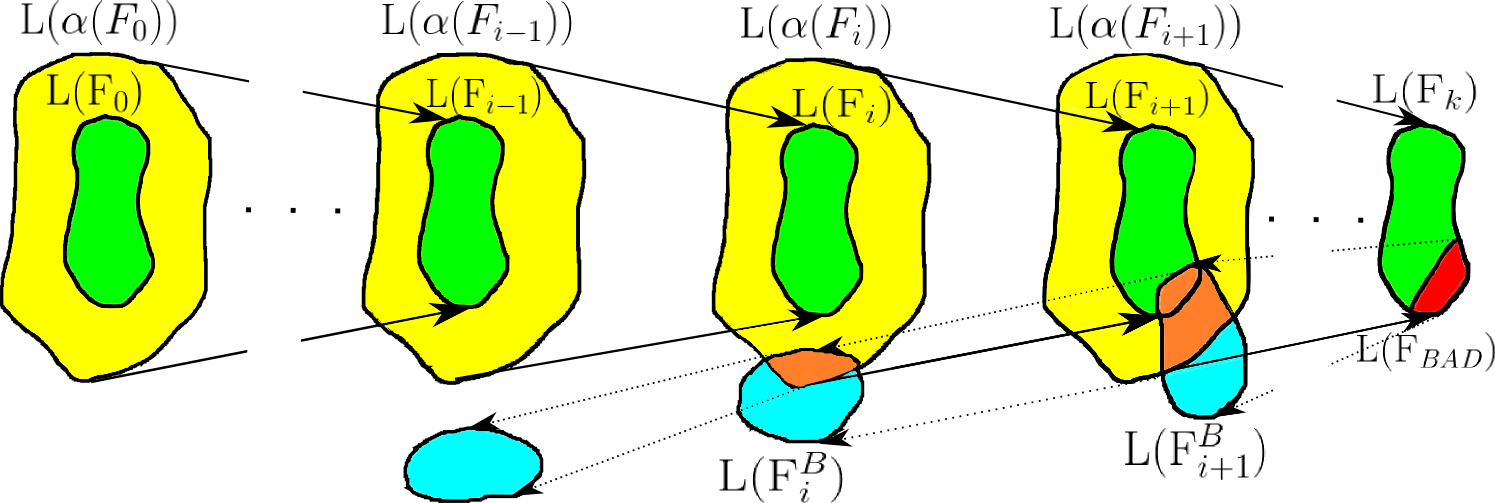
\includegraphics[width=\textwidth]{figs/artmc.png}
%	\caption{
%		Illustration (borrowed from \cite{artmc}) of the principles of the forward and the backward run and
%		the detection of a spurious counterexample.
%		}
%	\label{fig:bwrun}
%\end{figure}
%
Assume that the forward run $\fwrun = \sconf_0\sop_1\sconf_1\cdots\sop_n\sconf_n$ is spurious. 
Then there must be an index $i>0$ 
such that the symbolic path $\suffix \fwrun {i}$ is feasible 
but $\suffix \fwrun {i-1}$ is not.
This means that the operation $\sop_i$  over-approximated the semantics of~$\omega$ and 
introduced into~$\semof{\sconf_{i}}$ some heaps that are not in $\sopexiof{\semof{\sconf_{i-1}}}$ 
and that are \emph{bad} in the sense that they make $\suffix \fwrun {i}$ feasible.
%at the $i$th step. 
%
An \emph{interpolant for $\fwrun$}
%\td{OL: for sth? for the run $\fwrun$?} \tomas{Shouldn't it mention position $i$
%too? Usually, interpolants can be defined for any position of a spurious path. But for us, it is
%related to that unique one only, right? Perhaps to be mentioned so that people do not complain that we do not
%know what an interpolant is. In general, we should stress that our notion is
%special.}
is then a~forest automaton $\interp_i$ representing
%\td{OL: language?} 
the bad heaps
of $\semof{\sconf_i}$ that were introduced into $\semof{\sconf_{i}}$ by the
over-approximation in $\sop_i$ and are
disjoint from $\sopexiof{\semof{\sconf_{i-1}}}$.
% and does represent any configurations from $\sop_i$%
%\td{OL: I don't get it}
Formally,
%
\begin{enumerate}
\item
$\semof{\interp_i} \cap \sopexiof{\semof{\sconf_{i-1}}} = \emptyset$ and 
\item
$\fwrun_i$ is infeasible from all $\conf\in\semof{\sconf_i} \setminus \semof{\interp_i}$.
\end{enumerate}
%
%\td{OL: I still don't get why we're talking about the complement}
%
%\tomas{Not sure either. Couldn't we say that (1) $\semof{\interp_i} \supseteq
%\semof{\sop_i}{\semof{\sconf_{i-1}}}$ and (2) $\fwrun_i$ is infeasible from all
%$\conf\in \semof{\interp_i}$? That would be closer to the classical case, I
%think. But we get the other from the backward computation, right? So, then just
%again explain explicitly that it is so and that it is for pragmatic reasons.}

In the following, we describe how to use backward run, which reverts operations
of the forward run on the semantic level, to check spuriousness of an abstract
counterexample.
Moreover, we show how to derive interpolants from backward runs reporting
spurious counterexamples, and how to use those interpolants to refine the
operation of abstraction so that it will not introduce the bad configurations
in the same way again.
% In the following, we describe how to compute the interpolant using a backward run that reverts the operations on the semantic level, and how to use the interpolant to refine the operation of abstraction so that it will not introduce the bad configurations in the same way again.
%

A~\emph{backward run} for~$\fwrun$ 
is the sequence~$\bwrun = \bwsconf_0 \cdots \bwsconf_n$
such that
%
\begin{enumerate}
\item
$\bwsconf_n = \sconf_n$ 
and
\item
$\semof{\bwsconf_{i-1}} = \sopexiinvof{\semof{\bwsconf_{i}}} \cap \semof{\sconf_{i-1}}$, 
that is, ${\bwsconf_{i-1}}$ represents the \emph{weakest precondition} of
$\semof{\bwsconf_{i}}$ w.r.t.~$\sopexi$ that is \emph{localized} to
$\semof{\sconf_{i-1}}$.\vspace*{-0.5mm}
\end{enumerate}
%
If it happens that there is an FA $\bwsconf_i$ such that $\semof{\bwsconf_i} = \emptyset$ (and,
consequently, $\semof{\bwsconf_0} = \emptyset, \ldots, \semof{\bwsconf_{i-1}} =
\emptyset$), the forward run is spurious.
In such a~case,
an interpolant $\interp_i$ for $\fwrun$ can be obtained as $\bwsconf_{i+1}$ where $i+1$ is
the smallest index such that $\semof{\bwsconf_{i+1}}\neq~\emptyset$. 
%
We elaborate on the implementation of the backward run in
\secref{sec:CEXanalysis}.

We note that our use of interpolants differs from that of McMillan
\cite{mcmillanCAV03} in two aspects. First, due to the nature of our backward
run, we compute an interpolant over-approximating the source of the suffix of a
spurious run, not the effect of its prefix. Second, for simplicity of
implementation in our prototype, we do not compute a~sequence of localized
%implementation in our prototype tool, we do not compute a~sequence of localized
interpolants but use solely the interpolant obtained from the beginning of the
longest feasible suffix of the counterexample for a global refinement. 
%We note,
%however, that it would also be possible to use the sequence
%$\bwsconf_i,\ldots,\bwsconf_n$ as localized interpolants.
It would also, however, be possible to use the sequence
$\bwsconf_i,\ldots,\bwsconf_n$ as localized interpolants.


In \secref{sec:abstraction}, we show that
using the interpolant $\interp_{i}$, 
it is possible to refine regular abstraction $\sop_i$ (the only over-approximating operation)
%into $\sop_i'$ 
to exclude the spurious run.
%\tomas{Say that it guarantees progress of the analysis which is a notion
%commonly used in the related work.}
We can formulate \emph{progress guarantees} for the next iterations of the CEGAR loop. 
%
The formulation will refer to the notion of \emph{compatibility} of two FAs,
which intuitively means that the two FAs represent the heaps from the
intersection of their semantics in the same way: their boxes are folding the
same sub-heaps of the represented heaps and their TA components are
partitioning the represented heaps into the same tree components. 
We will define compatibility formally in Section~\ref{sec:compatibility}.
%
The progress guarantees are that  
\begin{enumerate}
\item
for any FA $\fa$ such that  
%$\sconf$ is forest compatible with $\sconf_{i-1}$
$\semof{\sconf}\subseteq\semof{\sconf_{i-1}}$ 
that is compatible with $\sconf_{i-1}$ %(as defined in \secref{sec:compatibility})
it holds that
$\semof{\sop_i(\sconf)} \cap \semof{\interp_i} = \emptyset$, and
%
%\tomas{I'm not getting this at all. What is $F$? The phrase ``in certain sense''
%sounds strange.}
\item
forward runs $\fwrun' = \sconf_0'\sop_1\sconf_1'\cdots\sop_n\sconf_n'$ such
that for all $1\leq j \leq n$, $\semof{\sconf_i'}\subseteq\semof{\sconf_i}$
and $\sconf_i'$ is compatible with $\sconf_i$ are excluded from the
ART.
\end{enumerate}
%
%
%Based on this, we can then give the following progress guarantee for the CEGAR loop.
%Let  $\fwrun$ languages entail $\fwrun' = \sconf_0'\sop_1'\cdots\sop_n'\sconf_n'$ if 
%$\langof{\sconf_i'}\subseteq\langof{\sconf_i}$ for all $0\leq i \leq n$. 
%\begin{equation
%\text{There can be at most $n-i$ futher forward runs language-entailed by $\fwrun$.}
%\text{No further run language-entailed by $\fwrun$ can be bad until $i$.}
%\end{equation}
%\bigskip
%
%
%
%\lukas{Add some discussion about guarantees on the semantic level: If folding folds the same subgraphs into the same boxes, then we have also high-level semantic guarantees analogous to the above low-level ones.}
%
%\lukas{how to call better the high-level/low-level/language semantics? Better names?}
%
%\lukas{good names for notions: abstract commands/abstract transformers/symbolic commands/symbolic transformers, operations/symbolic operations/... ?}

%\td{OL: talk about CEGAR here}

% \bigskip
% \bigskip
%\annot[ol]{rewritten Lukas's rewritten paragraph :-/}
In the following sections, we elaborate in a greater detail on the components
of the verification procedure outlined above. 
We discuss the construction of forest automata \emph{intersection} in \secref{sec:intersection},  
%We start by giving a~high-level view of how  we infer interpolants in our \emph{counterexample-guided
%abstraction refinement}
% (CEGAR) technique is used in our analysis
%(CEGAR; \secref{sec:interpolants}).
% accompanied by the description of \emph{intersection} of
% FAs (\secref{sec:intersection}).
then we describe how the \emph{forward run} is implemented
in \secref{sec:fwd_run}, 
and how operations are
inverted while checking spuriousness of a~counterexample in a~\emph{backward
run} in \secref{sec:CEXanalysis}.
We then discuss the \emph{regular abstraction} and its
\emph{refinement} using the interpolants obtained from the backward run
in \secref{sec:abstraction}.
Lastly, we give more detail on how \emph{boxes} to be folded are automatically identified within the
transformation-abstraction-folding loop in \secref{sec:box_discovery}.
%\annot[lh]{Update this description according to the actual structure!!!}

%*******************************************************************************
\section{Intersection of Forest Automata}
\label{sec:intersection}
%*******************************************************************************

The inference of interpolants used intersection of semantics of forest automata to
detect spuriousness of a~counterexample.
In this section, we give an algorithm that computes an under-approximation of
the intersection of semantics of a~pair of FAs, and later give conditions
(which are, in fact, met by the pairs of FAs in our backward run analysis) on
the intersected FAs to guarantee that the computed intersection is precise.

\subsection{Intersection Construction}
A simple way to compute 
%
the intersection of semantics of two FAs, denoted as $\cap$, is com\-po\-nent-wise, 
that is, for two hierarchical FAs $\fa = \tuple{\tas,\asgn}$ and $\fa' = \tuple{\tasprime,\asgn'}$ over $\tuple{\abcd, \gvars}$ with $\asgn=\asgn'$,
we compute the FA $\fa\cap\fa' =
\tuple{(\ta_1\cap\ta_1')\cdots(\ta_n\cap\ta_n'), \asgn}$ (intersection of forest automata with different numbers of components or different assignments of references is always empty).
%
The tree automata product construction for our special kind of tree automata
synchronizes on data values and on references.
That is, a~pair~$(a,b)$ that would be computed by a~classical product
construction where $a$ or $b$ is a reference or a data value is replaced by~$a$
if $a = b$, and removed otherwise (cf. \cite{tata} for the standard construction).
%
This  algorithm only under-approximates the actual semantic intersection, i.e., it is only guaranteed that $\semof{\fa\cap\fa'}\subseteq\semof\fa\cap \semof{\fa'}$.

To increase its precision, we replace the operator $\cap$ by the operator $\isectfa$, which takes into account the semantics of boxes.
%Namely, when synchronising two transitions in the TA product, it recursively calls intersection of forest automata.
%
Namely, we compute the FA $\fa\isectfa\fa'$ in a~similar way as $\fa\cap\fa'$, but replace the tree
automata product $\ta\cap\ta'$ by the construction of $\ta\isectta\ta'$, which recursively calls $\isectta$ on boxes.
For TAs $\ta = (Q, q_0, \Delta)$ and $\ta' = (Q',q_0', \Delta')$, it computes the  TA
$\ta\isectta\ta' = (Q \times Q', (q_0, q_0'), \Delta\isectta\Delta')$ where
$\Delta\isectta\Delta'$ is built as follows:
    %
    %\begin{align*}
    %\Delta\isectta\Delta' = \big\{ & \transover{(q, q')}{\edgesymb\isectta\edgesymb'}{(q_1, q'_1), \ldots,
    %  (q_m, q'_m)} \mid \transover{q}{\edgesymb}{q_1, \ldots, q_m}
    %  \in \Delta,\\
    %  &
    %  \transover{q'}{\edgesymb'}{q'_1, \ldots, q'_m} \in \Delta'
    %  \big\}.
    %\end{align*}
    %
    %Suppose $\edgesymb = a_1 \cdots a_m$, $\edgesymb' = a_1' \cdots
    %a_m'$, and that there is an index $0 \leq i \leq m$ such that if $
    %j \leq i$, $a_j$ and $a_j'$ are not boxes, and if $i < j
    %$, $a_j$ and $a_j'$ are boxes.
    %The vector of symbols $\edgesymb \isectta \edgesymb'$ is created as
    %$(a_1\isectta a_1') \cdots (a_m\isectta a_m')$ if $a_i\isectta a_i'$ is
    %defined for all $i$'s, otherwise the transition is not created.
    %The symbol $a_i\isectta a_i'$ is defined as follows:
    %%
    %\begin{enumerate}
    %  \item  for $j \leq i$, $a_j\isectta a_j'$ is defined as $a_j$ if $a_j = a_j'$ and is undefined otherwise,
    %  \item  for $j > i$, $a_j\isectta a_j'$ is the intersection of FAs (both
    %    $a_j$ and $a_j'$ are boxes, i.e., FAs).
    %\end{enumerate}
    \begin{align*}
    \Delta\isectta\Delta' = &\  \big\{  \transover{(q, q')}{a_1\isectfa a_1'\cdots a_n\isectfa a_n'}{(q_1, q'_1), \ldots,
      (q_m, q'_m)} \mid\\ & \transover{q}{a_1\cdots a_n}{q_1, \ldots, q_m}
      \in \Delta,
      \transover{q'}{a_1'\cdots a_n'}{q'_1, \ldots, q'_m} \in \Delta'
      \big\}.
    \end{align*} where the symbol $a_i\isectfa a_i'$ is computed as follows:
    %Suppose $\edgesymb = a_1 \cdots a_m$, $\edgesymb' = a_1' \cdots
    %a_m'$, and that there is an index $0 \leq i \leq m$ such that if $
    %j \leq i$, $a_j$ and $a_j'$ are not boxes, and if $i < j
    %$, $a_j$ and $a_j'$ are boxes.
    %The vector of symbols $\edgesymb \isectta \edgesymb'$ is created as
    %$(a_1\isectta a_1') \cdots (a_m\isectta a_m')$ if $a_i\isectta a_i'$ is
    %defined for all $i$'s, otherwise the transition is not created.
    %The symbol $a_i\isectta a_i'$ is defined as follows:
    %
    \begin{enumerate}
		\item If $a_i = a_i'$ then $a_i \isectfa a_i' = a_i$,  
      \item else if $a_i = B_{(i)}$ and $a_i' = B'_{(i)}$ where $B$ and $B'$ are boxes over $\tuple{\abcd,\gvars}$, 
				then $a_i\isectfa a_i' = (B\isectfa B')_{(i)}$,
		\item otherwise $a_i \isectfa a_i'$ as well as the whole transition is undefined (and no transition is added to $\Delta \isectta \Delta'$). 
    \end{enumerate}

% \vspace*{-1mm}\paragraph{Compatibility of forest automata.}
%-------------------------------------------------------------------------------
\subsection{Compatibility for Precise Intersection}\label{sec:compatibility}
%-------------------------------------------------------------------------------

In this section, we formally define the notion of \emph{compatibility} of FAs.
Compatibility is required in order to guarantee precision of intersection of FAs
from the forward and the backward runs.
Intuitively, it means that the heaps represented by the FAs are folded into
boxes in the same way.
If this were not the case, due to the different positions (or types) of boxes
occurring in the~FAs, the intersection operation might yield an FA with the
empty language, although intersection of the semantics of the FAs would be non-empty.

For a forest automaton $\fa = \tuple{\tas,\valuation}$, its version with \emph{marked components}
is the FA 
$\decof\fa = \tuple{\tas,\valuation\cup\valuation_\rootvar}$ 
where
$\valuation_\rootvar$ is the mapping $\{\rootvar_1\mapsto
1,\ldots,\rootvar_n\mapsto n\}$.
%
The \emph{root variables} $\rootvar_i$ are fresh variables that
point to the roots of the tree components in $\langof{\fa}$. 
%
$\semof{\decof\fa}$ then contains the same heaps as $\semof\fa$, but the
roots of the components from $\langof{\fa}$ remain visible, since they are explicitly marked by the root variables.
%
In other words, the root variables track how the forest decomposition of heaps
in $\langof{\fa}$ partitions the heaps from~$\semof{\fa}$. 
%
By removing the root variables of $\decof\heap\in\semof{\decof\fa}$, we get the
original heap $\heap\in\semof\fa$. We call $\decof\heap$ the \emph{component
decomposition of $\heap$ by~$\fa$}.

Using the notion of component decomposition, we further introduce a notion of
the \emph{representation} of a~heap by an FA. Namely, the \emph{representation}
of a~box-free heap~$\heap$ by an FA $\fa$ with $\heap\in\semof\fa$ records
how~$\fa$ represents~$\heap$, i.e., (i) how $\fa$ decomposes $\heap$ into
components, and (ii) how its sub-graphs enclosed in boxes are represented by the
boxes. 
%
Formally, the representation of~$\heap$ by~$\fa$ is a pair~$\repre =
(\decof\heap,\{\repre_1,\ldots,\repre_n\})$ such that $\decof\heap$ is the
component decomposition of $\heap$ by $\fa$, and $\repre_1,\ldots,\repre_n$ are
obtained from the sequence of unfoldings\vspace*{-0.5mm}
%
%\old{
%\begin{equation*} \heap_0\unfoldofi{1} \heap_1 \unfoldofi{2}  \cdots
%\unfoldofi{n} \heap_n \end{equation*}
%}
\begin{equation*} 
\heap_0
\unfoldof{\botox_{1}, u_{1}}{g_{1}} 
\heap_1
\unfoldof{\botox_{2}, u_{2}}{g_{2}} 
\cdots
\unfoldof{\botox_{n}, u_{n}}{g_{n}}   
 \heap_n 
\end{equation*}
%
with $\heap_0 = \decof\heap$ and $\heap_n\in\langof{\decof{\fa}}$, such that for
each $1\leq i\leq n$, $\repre_i$ is (recursively) the representation of $g_i$ in
$\botox_i$.

We write~$\semof\repre$ to denote $\{\heap\}$, and,
%
for a set of representations~$\repres$, we let $\semof\repres =
\ourbigcup_{\repre\in\repres} \semof{\repre}$.
% \{\semof\dec\mid\dec\in\decs\}$.
%
The set of \emph{representations accepted by a forest automaton} $\fa$
is the set $\represof\fa$ of all representations of heaps from
$\semof\fa$ by $\fa$. 
%
We say that a~pair of FAs $\fa$ and $\fa'$ is \emph{(representation) compatible} iff $\semof \fa \cap
\semof {\fa'} = \semof{\represof \fa \cap \represof{\fa'}}$.
%
The compatibility of a~pair of FAs intuitively means that for every heap from the semantic intersection of the two FAs,
at least one of its representations is shared by them.
%

\begin{lemma}
  For a pair $\fa$ and $\fa'$ of compatible FAs,
  it holds that
  $\semof{\fa \isectfa \fa'} = \semof{\fa} \cap \semof{\fa'}$.
\end{lemma}



%*******************************************************************************
\section{Implementation of the Forward Run}\label{sec:fwd_run}
%*******************************************************************************
%The main goal of this section is to describe the operations that are used to
%implement the forward symbolic execution over FAs. However, before that, we need
%to introduce one more notion that will subsequently allow us to implement the
%backward execution by inverting the operations used in the forward execution.
%%
%In particular, apart from the already introduced box compatibility, we need to
%introduce a further notion of component compatibility.
%%
%It is defined as follows.

This section describes the operations that are used to
implement the forward symbolic execution over FAs. 
%
%It is defined as follows.
%
%
% Namely, to be able to invert the operations used in a~forward run $\fwrun =
% \sconf_0\sop_1\cdots\sop_n\sconf_n$ (i.e., to compute the localized weakest
% preconditions over the run) and to compute an interpolant~$\interp_i$ of
% a~spurious run, which we need for refinement, we will require the backward run
% $\bwrun = \bwsconf_0 \cdots \bwsconf_n$ to compute $\bwsconf_j$ that is both
% box-compatible and component-compatible with $\sconf_j$ for every $i\leq j\leq
% n$.
%
% Box compatibility is important for the operation of intersection to be
% semantically precise, as discussed in Section~\ref{sec:intersection}, and also
% as a~prerequisite of component compatibility. Component compatibility is needed
% to invert the operations used in the forward run.
%
%\paragraph{Component decomposition.}
%For a forest automaton $\fa = \tuple{\tas,\valuation}$, its \emph{component
%semantics} is
%$\semcompof{\fa}=\semof{\tuple{\tas,\valuation\cup\valuation_\rootvar}}$ where
%$\valuation_\rootvar$ is the mapping $\{\rootvar_1\mapsto
%1,\ldots,\rootvar_n\mapsto n\}$.
%%
%% $\rootvar_i$'s are fresh \emph{root variables} 
%%
%%\tomas{Stress even more that the root variables point explicitly to each root.
%%Stress that this is meaningful when the roots need not be cut-points? I was
%%quite confused here for a while---I just hope it is for the case of having
%%non-cut-point roots.} \lukas{hm, maybe it is}
%%
%Here, the \emph{root variables} $\rootvar_i$ are fresh variables that are set to
%point to the roots of the tree components in $\langof{\fa}$. 
%%
%Then, $\semcompof{\fa}$ contains the same heaps as $\semof\fa$ but with the
%roots of the components from $\langof{\fa}$ explicitly marked by the root
%variables.
%%
%In other words, the root variables track how the forest decomposition of heaps
%in $\langof{\fa}$ partitions the heaps from~$\semof{\fa}$. 
%%
%The elements from $\semcompof{\fa}$ are called \emph{component decompositions}.
%%
%For a~set~$S$ of component decompositions, we can come back to the standard semantics
%by removing the root variables, which is denoted by~$\semofcd{S}$.
%%
%We say that two forest automata~$\fa$ and~$\fa'$ are \emph{component-compatible} iff
%$\semof{\fa}\cap\semof{\fa'} = \semofcd{\semcompof\fa\cap\semcompof{\fa'}}$.
%%
%Intuitively, it means that the heaps in the semantic intersection have the same
%sub-heaps encoded by the components of the FAs at the same
%positions.
%
To be able to implement the backward run, we will need to maintain
compatibility of the FAs (discussed in the previous section) between the forward run and
the so-far constructed part of the backward run.
%
Therefore, we will present the operations used in the forward run mainly from
the point of view of their effect on the representation  of heaps (in the sense
of \secref{sec:compatibility}).
%
Then, in \secref{sec:CEXanalysis}, we will show how this effect is inverted in
% Then, in \secref{sec:bwd_run}, we will show how this effect is inverted in
the backward run such that, when starting from compatible
configurations, the inverted operations preserve compatibility of the
configurations in the backward run with their forward run counterparts.

% we get to compatible configurations again, and
% hence compatibility is preserved in the backward run.


%Now, we are finally ready to describe the operations used in the forward run.
%We are now ready to describe the operations used in the forward run.
%
We omit most details of the way the operations are implemented on the level of
manipulations with transitions and states of FAs. 
%We mostly omit their detailed implementation on the level of manipulations with
%rules and states of FAs. 
%since it is not important for this paper; instead,
%we refer the reader to~\cite{forester12,jiri:diza} for details.
We refer the reader to~\cite{habermehl:forest,jiri:diza} for the
details.

We note that when we talk about removing a~component or inserting a~component
in an FA, this also includes renaming references and updating
assignments of variables.
%
When a~component is inserted at a~position~$i$, all references to~$\rr j$ with
$j \geq i$ are replaced by~$\rr{j+1}$, including the assignment~$\asgn$ of variables.
%
When a~component is removed from a~position~$i$, all references to~$\rr j$ with $j > i$ are
replaced by references to~$\rr{j-1}$. 


% To revert the operations, we will sometimes need to remember some operation
% from the forward run in the backward run.
% We make that information visible in a~form of a~parameter $\mathit{par}$ of the
% operation, which will be in the form $\sop[\mathit{par}]$.

%which are generalization that consists of regular abstraction, normalization, and folding, 
%and operations that implement program statements.

%
%To explain the computation of localized preconditions while preserving the forest compatibility invariant,
%we will present the operations divided into smaller instructions,
%which affect forest compatibility.
%
%In the previous section we describe it on level of forest automata languages.
%To enable predicate learning described in the previous section we need to perform
%a backward run on level of compatible forest decomposition represented by automata
%from the forward and backward run.
%Therefore we provide with more detailed description of what happens in forward run
%with FA. The we will describe how we revert the operations from forward run in backward run.

%-------------------------------------------------------------------------------
\subsubsection*{Splitting}\label{sec:label}
%-------------------------------------------------------------------------------
% \paragraph{Splitting.}
Splitting has already been discussed in \secref{sec:analysis}.
It splits the symbolic execution into several branches such that the union of
the FAs after the split is semantically equivalent to the original~FA.
%
The split is usually performed when transforming an~FA into several FAs that
have only one variant of a~root transition of some of their components.
%
From the point of view of a~single branch of the~ART,
splitting is an operation, denoted further as $\splitting$, that transforms an
FA $\fa$
into an FA~$\fa'$ s.t. $\semof{\fa'}\subseteq\semof\fa$ and 
$\represof{\fa'}\subseteq\represof\fa$.
Therefore, $\fa$ is compatible with~$\fa'$.

%*******************************************************************************
% \subsection{Auxiliary Operations over Forest Automata}\label{sec:label}
\subsubsection*{Operations Modifying Component Decomposition}\label{sec:opdec}
% \subsection{Operations Modifying Component Semantics}\label{sec:label}
%*******************************************************************************
% \paragraph{Operations Modifying Component Semantics}
% \comment[ol]{the title is strange}
% \paragraph{Operations modifying component decomposition.}
This class of operations is used to implement transformation of FAs to the dense form and as
pre-processing steps before the operations of folding, unfolding, and symbolic
implementation of program statements.
%
They do not modify the semantics of forest automata, 
but change the component decomposition of the represented heaps.
%Folding and unfolding of boxes and implementations of program commands need preprocessing of the forest automata so that their component semantics satisfies certain properties. The preprocessing is done by a set of operations that modify the component semantics, while not modifying the box semantics.
%
\begin{itemize}
%\item[\emph{Component Removal.}]
%Removing the $i$th component requires also replacing all references to $j$th components for $j>i$ by references to $j-1$th component, in the languages of the tree automata as well as in the valuation of variables.
%Removing appear in a forward run as $\removing{i}$.
%Normalization does not change forest automata semantically, 
%but affects the component decomposition of their heaps.
%

%Splitting is done when an operation such as $\code{x = y\text{\texttt{->}}sel}$ is performed.
%Since a forest automaton can represent a set of heaps this operation could cause that
%their forest decomposition differ. E.g. consider a cyclic singly linked list
%of arbitrary length where \code{y} points to a head of list.
%Then the noted operation would result to (a) at least two tree components for
%length longer than one or (b) one tree component for list of length one.
%Forest automata are not capable of representation of such different heaps.
%Therefore we create (split) more copies of automaton, one for each possible tree decomposition.
%The symbolic execution is then split to the separated branches for particular
%forest automata and each branch continues independently.
% \item[\emph{Connecting of components.} ] 
\item \emph{Connecting of components.}
%\tomas{This name sounds extremely strange to me. Perhaps Connecting a Component?}
When the $j$-th component $\ta_j$ of a forest automaton $\fa$ accepts trees with false roots, 
then $\ta_j$ can be connected to the component that refers to it. 
%
Indeed, as such roots are not cut-points, 
a~reference $\rr j$ to them can appear only in a~single component, say $\ta_k$, 
and at most once in every tree from its language (because a~false root
can have at most one incoming edge). 
%
For simplicity, assume that~$\ta_j$ has only one root state~$q$, which does
not appear as a~child state in transitions.
%
The connection is done by adding the states and transitions of~$\ta_j$ to~$\ta_k$,
replacing the reference~$\rr j$ in the transitions of~$\ta_k$ by~$q$.
%From the language point of view, the trees of $\ta_j$ are thus 
%reference $\bar j$ 
%connected to roots of the trees of $\ta_i$.  
%
The $j$-th component is then removed from~$\fa$.
%
The previous sequence of actions is below denoted as the operation $\connecting{j,k,q}$. 
%
%
%It is done by replacing the reference $\bar i$ at the right-hand side of a leaf rule by the root state $q$ of $\ta_i$.  
%The $i$th component is removed by $\removing{i}$.
%The connection then appears in the forward run
%as the operation $\connecting{q,i}$. 
%\lukas{state maybe not needed to remember}
% \item [\emph{Cutting of a component.}] 
\item \emph{Cutting of a component.}
Cutting splits a~component with an index~$j$ into two. 
The part of the $j$-th component containing the root will accept tree prefixes
of the original trees, and the~new $k$-th component will accept their remaining
sub-trees.
%of them is accepting subtrees of the trees accepting by the original one, and the other one is accepting tree prefixes that have a reference to the sub-tree component at the place where the sub-tree was connected.  
The cutting is done at a state $q$ of $\ta_j$, which appears exactly once in
each run (the FA is first transformed to a~form that satisfies this). 
Occurrences of~$q$ as child states of transitions are replaced by the
reference~$\rr k$ to the new component, and $q$~becomes the root state of the new
component. 
We denote this operation by $\cutting{j,k,q}$.
%The information about $q$ and $i$ together with the assumption about $q$ will allow us to revert it in the backward run. 
% \item [\emph{Swapping of components.}]
% \annot[lh]{the output references must be then shifted}
\item \emph{Swapping of components.}
  The operation $\swapping{j,k}$ swaps the
  $j$-th and the $k$-th component (and renames references and assignments
  accordingly). 
\end{itemize}

%%%%   \subsection{Normalization}
%%%%   Calling normalisation is important because (1) 
%%%%   it facilitates the entailment checking \cite{cav} used to detect the fixpoint of the symbolic execution, 
%%%%   (2) it merges tree automata components, keeping their number small, which is important for efficiency reasons, and 
%%%%   (3) it empowers regular abstraction, which has more opportunities to overapproximate if the heaps are decomposed to a small number of large components.   
%%%%   %On forest automata representations with less tree components, because it is applied to tree components in isolation, and having larger pieces of configurations within a single component gives it more opportunities to overapproximate.
%%%%   %
%%%%   A detailed description of normalization can be found in \cite{cav,jiri,martin}. 
%%%%   It can be implemented as a sequence of operations of three kinds:
%%%%   \begin{itemize}
%%%%   \item [\emph{Splitting.}] As discussed in Section~\ref{}, it splits the symbolic execution into several branches. 
%%%%   From a point of view of single branch/forward run, 
%%%%   it appears as an operation $\splitting$ which transforms a forest automaton $\fa$ into $\fa'$ such that, $\semof\fa'\subseteq\semof\fa$, 
%%%%   and which is box and component compatible with $\fa$ because splitting does not influence the decomposition and component semantics.
%%%%   %Normalization does not change forest automata semantically, 
%%%%   %but affects the component decomposition of their heaps.
%%%%   %
%%%%   
%%%%   %Splitting is done when an operation such as $\code{x = y\text{\texttt{->}}sel}$ is performed.
%%%%   %Since a forest automaton can represent a set of heaps this operation could cause that
%%%%   %their forest decomposition differ. E.g. consider a cyclic singly linked list
%%%%   %of arbitrary length where \code{y} points to a head of list.
%%%%   %Then the noted operation would result to (a) at least two tree components for
%%%%   %length longer than one or (b) one tree component for list of length one.
%%%%   %Forest automata are not capable of representation of such different heaps.
%%%%   %Therefore we create (split) more copies of automaton, one for each possible tree decomposition.
%%%%   %The symbolic execution is then split to the separated branches for particular
%%%%   %forest automata and each branch continues independently.
%%%%   \item[\emph{Connecting.}] 
%%%%   When the root of an $i$th component $\ta_i$ of a forest automaton $\fa$ does not semantically correspond to a cut-point, 
%%%%   then the component is merged with other components. 
%%%%   From the language point of view, 
%%%%   the trees from $\langof{\ta_i}$ are connected as sub-trees to trees accepted by the other components at their leaves with a reference to $i$th component. 
%%%%   %
%%%%   It is done by replacing the reference $\bar i$ at the right-hand side of a leaf rule by the root state $q$ of $\ta_i$.  
%%%%   The connection then appears in the forward run
%%%%   as the operation $\connecting{q,i}$. 
%%%%   \lukas{state maybe not needed to remember}
%%%%   %The information about $q$ and $i$ together with the assumption about $q$ will allow us to revert it in the backward run. 
%%%%   \item [\emph{Swapping.}] 
%%%%   Tree automata components are swapped to achieve canonic ordering. 
%%%%   The operation appears as $\swapping{i,j}$, 
%%%%   where $i,j$ are indices of the swapped components. 
%%%%   \end{itemize}

%*******************************************************************************
\subsubsection*{Folding of Boxes}\label{sec:box_folding}
%*******************************************************************************


In this section, we briefly describe the effect of folding FAs into boxes during our
symbolic execution.
More details and algorithms for selecting which part of which components of FAs are
to be folded will be given in \secref{sec:box_discovery}.

The folding operation assumes that the concerned FA is first transformed into the form
$\fa = \tuple{\boxtas \ta_1' \cdots \ta_m',\asgn}$ by a~sequence of splitting,
cutting, and swapping.
The tuple of tree automata $\boxtas$ will then be folded into a~new $k$-ary
box~$\botox$ with~$\ta_\iport$ as its input component and~$\ta_{\oport_1},
\ldots, \ta_{\oport_k}$ as its outputs.
Moreover, the operation is given sets of selectors~$S_{\iport},
S_{\oport_1}, \ldots, S_{\oport_k}$ of roots of components in~$\ta_\iport$
and~$\ta_{\oport_1}, \ldots, \ta_{\oport_k}$, respectively, that are to be folded
into~$\botox$.
%
The box~$\botox =
\tuple{\boxtasin,\{\iport\mapsto 1,\oport_1\mapsto \mbox{$n-k+1$}, \ldots, \oport_k
\mapsto n \}}$
 arises from~$\fa$ by taking the tuple of tree automata $\boxtas$
%
and removing selectors that are not in~$S_{\iport}$ and~$S_{\oport_1},
\ldots, S_{\oport_k}$
from the root transitions of~$\ta_\iport$ and~$\ta_{\oport_1}, \ldots, \ta_{\oport_k}$ to obtain $\ta_\iport^\botox$ and
$\ta^\botox_{\oport_1}, \ldots, \ta^\botox_{\oport_k}$, respectively (we w.l.o.g. assume that the root states of the TAs do not appear as child states in transitions).

Folding returns the forest automaton $\fa' = \tuple{\ta'_{\iport}
\ta'_{\oport_1} \cdots \ta'_{\oport_k} \ta'_1 \cdots \ta'_m, \asgn'}$ that arises from $\fa$ as follows.
All successors of the roots accepted in $\ta_\iport$ and $\ta_{\oport_1},
\ldots, \ta_{\oport_k}$
reachable over selectors from $S_\iport$ and $S_{\oport_1}, \ldots, S_{\oport_k}$
are removed in $\ta'_\iport$ and $\ta'_{\oport_1}, \ldots, \ta'_{\oport_k}$,
respectively (since they are enclosed into~$\botox$).
The root of the trees of $\ta'_\iport$ gets an additional edge labelled by
$\botox$, leading to the reference $\rr n$ (the output port),
and the components $\ta_2, \ldots, \ta_{n-1}$ are removed (since they are also enclosed in~$\botox$).
%
This operation is denoted as $\folding{n,S_{\iport},S_{\oport_1}, \ldots, S_{\oport_k},\botox}$.

%*******************************************************************************
\subsubsection*{Unfolding of Boxes}\label{sec:box_unfolding}
%*******************************************************************************

Unfolding is called as a preprocessing step before operations that implement
program statements
in order to expose the selectors accessed by the statement. 
Before an unfolding is performed, the input FA with a~$k$-ary box~$\botox$ is first transformed
(using a sequence of cutting, splitting, and swapping)
into the form
$\fa' = \tuple{\ta_\iport'\kword{\ta_{\oport_{#1}}'}\ta_1'\cdots\ta_m',\asgn'}$
where
the roots of the trees accepted by~$\ta'_\iport$ have an outgoing
$\botox$-labeled hyperedge to references
%$\kseq{\overline {1+{#1}}}$
$\overline {2},\ldots,{\overline{k+1}}$.
%to $\kseq{\ta_{\oport_{#1}}'}$ accessible by a 
%heaps $\heap$ and~$\heapp$, the heap $\heapp$ is an \emph{unfolding} of $\heap$
%if there is an hyperedge of $\heap$ of a $k$-ary box $\botox$ from a node $\node$ 
%hyperedge going from the root and labelled by the box~$\botox$ that is to be unfolded.
%
Furthermore, assume that the box $\botox$ is of the form
$\tuple{\boxtasin,\{\iport\mapsto 1,\oport_1 \mapsto n-k+1, \ldots, \oport_k \mapsto n\}}$
%
and 
%
the ports have outgoing edges with selectors from the sets 
$S_\iport$ and $\kseq{S_{\oport_{#1}}}$ respectively. 
%
The operation returns the forest automaton~$\fa$ that arises from~$\fa'$ by 
%$\tuple{\ta_\iport'',\tas,\ta_\oport'',\{\iport\mapsto 1,\oport\mapsto n+1\}}$
%
inserting components $\boxtasin$ in between $\ta'_\iport$ and
% $\kseq{\ta'_{\oport_{#1}}}$, 
$\ta'_{\oport_{1}}$, 
removing the $\botox$-transition
% (all the $k$~edges constituting it),
including its targets, 
%successor of the root in~$\ta_\iport'$,
and merging~$\ta_\iport^\botox$ with~$\ta_\iport'$ and $\kseq{\ta_{\oport_{#1}}^\botox}$
with $\kseq{\ta_{\oport_{#1}}'}$ respectively.
% The merging on the language level consists of merging roots of the trees.
The merging on the TA level consists of merging root transitions of the
corresponding TAs.
%
We denote this operation as $\unfolding{n,S_{\iport},\kseq{S_{\oport_{#1}}},\botox}$.\footnote{The parameters $S_{\iport},\kseq{S_{\oport_{#1}}}$ are used  in the backward run to easily invert the operation of unfolding by folding, cf. \secref{sec:bwd_run}.}



%*******************************************************************************
\subsubsection*{Symbolic Execution of Program Statements}\label{sec:label}
%*******************************************************************************
% \paragraph{Symbolic Execution of Program Statements.}

We will now discuss our symbolic implementation of the most essential statements
of a C-like programming language. 
%They are 
%$\code{x = malloc()}$, 
%$\code{x = y\text{\texttt{->}}sel}$,
%$\code{y\text{\texttt{->}}sel = x}$,
%$\code{y \datarel x}$,
%$\code{x = y}$ or $\code{x = NULL}$, and
%$\code{free(y)}$.
%%
%Symbolic implementations of the statements use four operations. 
%%
%We use $\xroot$ and $\yroot$ to denote
%		the root states of $\xta$ and $\yta$, respectively. 	    
%
%
%The commands always access only selectors of nodes pointed to by variables.
%These are either exposed in root rules of the tree automata of the variable, in which case folding is not needed, or folded within a box. It is either a box in the root rule of $\valuation(x)$ or it may be a box
%within leaf rule which ends by a reference to the $\valuation(x)$. 
%In the latter case, 
%the occurrence of the box is first isolated into a separate tree component which contains the only the rule with the box. 
%
%It is unfolding, 
%which is to extract selectors of memory cells accessed by the statement from boxes, 
%then splitting, which is is necessary to keep the forest automata well define (??) 
%due to forest automata not being closed under union,
%and cutting.
%After preprocessing by unfolding and splitting and cutting, which have no semantic effect,
%the transformation changing the semantics is finally applied.
%We discuss the three in a more detail.
%
%
%Therefore we create (split) more copies of automaton, one for each possible tree decomposition.
%The symbolic execution is then split to the separated branches for particular
%forest automata and each branch continues independently.
%
%\paragraph{Abstract statement}
%
We assume that the operations are applied on an FA~$\fa = \tuple{\tas,\valuation}$.
		\begin{itemize}
		   \item $\code{x := malloc()}$: A new $(n+1)$-th component 
		  $\ta_{\mathit{new}}$ is appended to $\fa$ s.t. it contains one state and one transition with all
		  selector values set to $\asgnof \unef$.
      The assignment~$\asgnof{\code{x}}$ is set to the root reference~$\rr{n+1}$. 
		  %The operation basically adds one node $v$ to heaps from
		  %language of $\fa$ and sets $\asgnheapof{\code{x}}$ to $v$ for each heap $h$.

		  \item $\code{x := y\text{\texttt{->}}sel}$ and $\code{y\text{\texttt{->}}sel := x}$:
		% If $\valuationof{\code y} = \valuationof\unef$, then $\code{x = y\text{\texttt{->}}sel}$ moves to the error location.
		If $\valuationof{\code y} = \valuationof\unef$, the operation moves to the error location.
        Otherwise, by splitting, cutting, and unfolding, $\fa$~is transformed into the
        form where $\ta_{\asgnof{\code{y}}}$ has only one root transition and
        the transition has a~$\code{sel}$-successor that is a~root reference~$\rr j$. 
        The statement
$\code{x := y\text{\texttt{->}}sel}$ then changes $\valuationof{\code{x}}$ to $\rr j$, and
$\code{y\text{\texttt{->}}sel := x}$ changes the reference $\rr j$ in $\ta_{\asgnof{\code y}}$ to $\valuationof{\code x}$.

%$ \cval$We then only 
%          If $q_i$ is a root reference (say,
%		  $j$), it is sufficient to change the value of $\valuation(\code{x})$ to $j$.
%		  Otherwise, we split $\yta$ at the $i$-th position (creating $\ta_k$) and assign $k$ %to
%		  $\valuation(\code{x})$. This operation does not change language of a forest automaton
%		  but it can change forest decompositions of heaps. This is caused by possibility of
%		  creating a new cutpoint by redirection of variable $\code{x}$.

%		  \item[$\code{y\text{\texttt{->}}sel = x}$] 
%If $q_i$ is a state, then we split
%		  $\yta$ at the $i$-th position. Then we put a reference to ${\valuation(\code{x})}$ to the
%		  $i$-th position in the right-hand side of the root transition of $\yta$; this
%		  is done both if $q_i$ is a state and if $q_i$ is a root reference. The operation
%		  changes heaps from language of FA by redirecting the edges corresponding to
%		  the $\code{sel}$ selector.

      \item $\code{assume(x \datarel y)}$ where $\datarel\ \in \{\code{==},
        \code{{!}{=}}\}$:
        This statement tests the equality of $\valuation(\code{x})$ and $\valuation(\code{y})$
        and stops the current branch of the forward run if the result does not match $\datarel$.
      \item $\code{assume(x\text{\texttt{->}}data \datarel y\text{\texttt{->}}data)}$
        where $\datarel$ is some data comparison:
        We start by unfolding and splitting $\fa$ into the form where
        $\ta_{\valuation(\code{x})}$ and $\ta_{\valuation(\code{y})}$ have only
        one root transition with exposed $\code{data}$ selector.
        The data values at the $\code{data}$ selectors are then compared and
        the current branch of the forward run is stopped if the values do not satisfy~$\datarel$.
        The operation moves to the error locations if $\asgnof{\code x}$ or
        $\asgnof{\code y}$ are equal to~$\asgnof \unef$.
% \lukas{in the initial conf, everybody is defined and has the same value as undef, except null}
%with $\datarel$ and the forward run is stopped if the test returns false.  

%The is implemented by splitting the $\fa$ into all variants such that in each of them, both $\ta_\valuation{\code{x}}$ and  
%$\ta_\valuation{\code{y}}$ have a unique root rule and then removing the variants where the 
%		  Assume that both states are data ones.
%		  If $data_y \datarel data_x$ holds (or does not hold), we return \emph{true} (or \emph{false}).
%		  Otherwise, we copy $\tuple{\valuation, \fa}$ into two abstract configurations:
%		  $\tuple{\valuation, \fa_{\mathit{true}}}$ for the $\emph{true}$ branch and
%		  $\tuple{\valuation, \fa_{\mathit{false}}}$ for the $\emph{false}$ branch
%		  and continue from each branch separately. Operation does not change language of FA
%		  neither accepted forest decomposition.

		  \item $\code{free(x)}$:
        % The component $\ta_{\asgnof{\code{x}}}$ is removed, 
        %   and all references to $\asgnof{\code{x}}$ are replaced by~$\asgnof \unef$.
        First, we cut $\xta$ at all positions that appear in its root
        transition, then we remove $\xta$ from $\fa$ and set
        $\valuation(\code{x})$ to $\asgnof \unef$. 
      % \ol{this is unsound (garbage can leak), because the root transition
      %     isolation needs to be done first. Why was the previous sentence in the
      %     source commented out?}
		\end{itemize}

\noindent
The updates are followed by checking that all components are reachable from
program variables in order to detect garbage.
If some component is unreachable, the execution either moves to the
error location, or---if the analysis is set to ignore memory leaks---removes the
unreachable component and continues with the execution.

% %------------------------------------------------------------------------------
% \paragraph{Regular Abstraction.} 
% %Regular abstraction is implemented as one of the abstractions described in
% %Sec.~\ref{sec:abstraction}, which over-approximate the language of the
% %individual components.
% %It is preceded by a~transformation to the dense form 
% %by connecting and splitting the FA.
%
% Regular abstraction is described in
% Sec.~\ref{sec:abstraction}.
% It is preceded by a~transformation to the dense form 
% by connecting and splitting the FA.

% Our refinement on abstraction is based on the framework of
% \emph{counter-example guided abstraction refinement} (CEGAR)
%
%
% \td{OL: talk about abstraction here}
%
% \td{OL: talk about folding here}
% a little
% \cite{boxes13}


% The previous algorithm generates forward runs in the analyzed program \td{OL: blah}
% \td{OL: talk about CEGAR}
%

%For every command $\transf\in\transfs$, 
%the symbolic operation $\stransf$ is its symbolic version such that 
%$\cup_{\sconf'\in \stransf(\sconf)}\semof{\sconf'} = \{\transf(\conf)\mid\conf\in\semof{\sconf}\}$.
%Unfolding is, as folding, semantically identity. 
%On the level of languages, it maps configurations to their more unfolded versions.
%

%\td{OL: move this elsewhere}
%Our implementation in \forester{} explores the tree depth first.%\lukas{say this elsewhere?}  
%\td{OL: how about the DFS? we should emphasize it, because for other search order, this termination property might make the analysis unsound}

%%%%%%%%%%%%%%%%%%%%%%%%%%%%%%%%%%%%%%%%%%%%%%%%%%%%%%%%%%%%%%%%%%%%%%%%%%%%%%%%
% \section{Counterexample Analysis and Abstraction Refinement}\label{sec:CEXanalysis}
%\section{Backward Run for Counterexample Analysis}\label{sec:CEXanalysis}
\section{Abstraction and Counterexample-based Refinement}\label{sec:CEGAR}
%%%%%%%%%%%%%%%%%%%%%%%%%%%%%%%%%%%%%%%%%%%%%%%%%%%%%%%%%%%%%%%%%%%%%%%%%%%%%%%%
In this section, we will describe the complete counterexample-based refinement loop (CEGAR) for forest automata.
It is a~generalisation of the CEGAR for abstract regular tree model checking of~\cite{bhrv06a,bhrv06b}. 

%\annot[lh]{a coppy of vmcai intro. Some parts are a good description of refinement and backward run that can be used}
%In~\cite{forester12,boxes13}, \emph{forest automata} (FAs) were proposed as a
%formalism for representing sets of heap graphs within a fully-automated and
%scalable \emph{shape analysis} of programs with complex \emph{dynamic linked
%data structures}. FAs were implemented in the \forester{} tool and successfully
%used to verify programs over a wide range of data structures, such as different
%kinds of lists (singly- and doubly-linked, circular, nested, and/or having
%various additional pointers), different kinds of trees, as well as skip lists.
%FAs have the form of tuples of \emph{tree automata} (TAs), allowing abstract
%transformers corresponding to heap operations to have a \emph{local impact}
%(i.e., to change just a few component TAs instead of the entire heap
%representation), leading to scalability. To handle complex nested data
%structures, FAs may be \emph{hierarchically nested}, i.e., lower-level FAs can
%be used as (automatically derived) alphabet symbols of higher-level FAs.

\subsection{Backward Run for Counterexample Analysis}\label{sec:CEXanalysis}

Our counterexample trace validation is based on \emph{backward symbolic execution} of
a candidate counterexample trace on the level of FAs (with no abstraction on the
FAs) while checking \emph{non-emptiness of its intersection} with the forward
symbolic execution (which was abstracting the FAs). For that, we have to revert
not only abstract transformers corresponding to program statements but also
various meta-operations that are used in the forward symbolic execution and that
significantly influence the way sets of heap configurations are represented by
FAs. In particular, this concerns \emph{folding} and \emph{unfolding} of boxes
as well as \emph{splitting}, \emph{merging},
and \emph{reordering} of component TAs, which is used in the forward run for the
following two reasons: to
prevent the number of component TAs from growing and to obtain a canonic
FA representation. 

If the above meta-operations were not reverted, we would not only have problems
in reverting some program statements but also in intersecting FAs obtained from
the forward and backward run. Indeed, the general problem of checking emptiness
of intersection of FAs that may use different boxes and different component TAs
(i.e., intuitively, different decompositions of the represented heap graphs) is
open. When we carefully revert the mentioned operations, it, however, turns out
that the FAs obtained in the forward and backward run use \emph{compatible}
decompositions (cf.~\secref{sec:compatibility}) and hierarchical structuring of heap graphs, and so checking
emptiness of their intersection is possible. Even then, however, the
intersection is not trivial as the boxes obtained in the backward run may
represent smaller sets of sub-heaps, and hence we cannot use boxes as symbols
and instead have to perform the intersection \emph{recursively} on the boxes as
well.

The analysis of spurious counterexamples is further used to refine the abstraction. 
%
Particularly, we use a modification of the so-called \emph{predicate
language abstraction} on TAs~\cite{artmc}, which 
collapses those states of component TAs that
have non-empty intersection with the same predicate languages, which are
obtained from the backward run.
%
In case the intersection of the set of configurations of the above described forward and backward symbolic runs
is empty, we can derive from it an \emph{automata interpolant} allowing us to
get more predicate languages and to refine the abstraction such that progress of
the CEGAR loop is guaranteed (in the sense that the same
abstract forward run is not repeated).
%\comment[ar]{* -- End of the complete change}

%We have implemented the proposed approach in \forester{} and tested it on a
%number of small but challenging programs. Despite there is, of course, a lot of
%space for further optimisations, the experimental results are 
% 
% simply amazing (no need to be unnecessarily humble).
%
%very encouraging.
%
%\forester{} can now not only verify correct programs with complex dynamic data
%structures but also reliably report errors in such programs. For some classes of
%dynamic data structures (notably skip lists), \forester{} is, to the best of our
%knowledge, the only tool that can provide both sound verification as well as
%reliable error reporting in a fully automated analysis (i.e., no manually
%provided heap predicates, no invariants, etc.). Moreover, for some classes of
%programs (e.g., various kinds of doubly-linked lists, trees, and nested lists),
%the only other tool that we are aware to be able to provide such functionality
%is our older automata-based tool \cite{bhrv06b}, which is, however, far less
%scalable due to the use of a~monolithic heap encoding based on a single TA. 
%\comment[ar]{Kick out the rest till end of the section} Finally,
%the refinement mechanism we introduced allowed us to verify some programs that
%were before out of reach of \forester{} due to handling finite domain data
%stored in the heap (which can be used by the programs themselves or introduced
%by tagging selected elements in dynamic data structures when checking properties
%such as sortedness, reordering, etc.).


%%%%%%%%%%%%%%%%%%%%%%%%%%%%%%%%%%%%%%%%%%%%%%%%%%%%%%%%%%%%%%%%%%%%%%%%%%%%%%%%
\subsubsection*{Inverting Operations in the Backward Run}\label{sec:bwd_run}
%%%%%%%%%%%%%%%%%%%%%%%%%%%%%%%%%%%%%%%%%%%%%%%%%%%%%%%%%%%%%%%%%%%%%%%%%%%%%%%%

We now present a description of how we compute the weakest localized preconditions
(\emph{inversions} for short) of the operations from \secref{sec:fwd_run} in the backward run.
As mentioned in \secref{sec:fwd_run}, 
it is crucial that compatibility with the forward run is preserved. 
Let $\sconf_i = \sop(\sconf_{i-1})$ appear in the forward run and
$\bwsconf_{i}$ be an already computed configuration in the backward run
s.t.~$\sconf_i$ and $\bwsconf_i$ are compatible.
We will describe how to compute $\bwsconf_{i-1}$ such that it is also
compatible with~$\sconf_{i-1}$.

Inverting most operations is straightforward.
The operation $\cutting{j,k,q}$ is inverted by $\connecting{k,j,q_k}$ where $q_k$ is the root state of $\ta_k$,
$\swapping{j,k}$ is inverted by $\swapping{k,j}$, and $\splitting$ is not inverted, i.e., $\bwsconf_{i-1} = \bwsconf_i$.

One of the more difficult cases is 
$\connecting{j,k,q}$. %$\bwsconf_{i-1}$ is computed as follows. 
Assume for simplicity that $k$ is the index of the last component of~$\sconf_{i-1}$.
%
Connecting can be inverted by cutting, but prior to that, we need to find
\emph{where} the $k$-th component of $\bwsconf_i$ should be cut.
To find the right place for the cut, we will
use the fact that the places of connection are marked by the
state~$q$ in the FA $\sconf_i$ from the forward run.
%
We use the tree automata product $\isectta$ from
\secref{sec:intersection}, which
propagates the information about occurrences of $q$ to $\bwsconf_{i}$,
to compute the product of the $k$-th
component of $\sconf_{i}$ and the $k$-th component of~$\bwsconf_i$.
%
We replace the $k$-th component of $\bwsconf_i$ by the product, 
which results in an intermediate FA~$\bwsconf_i'$.
%
The product states with the first component $q$ now mark the places where the forward run connected the components (they were leaves referring to the $k$-th component).
%
This is where the backward run will cut the components to revert the connecting. 
%
Before that, though, we replace the mentioned product states with $q$ by a new state~$q'$.
This replacement does not change the language because $q$ was appearing
exactly once in every run (because in the forward run, it is the root state of
the connected component that does not appear as a~child state of any transition), therefore, 
a product state with $q$ can appear at most once in
every run of the product too.
%
Finally, we compute $\bwsconf_{i-1}$ as $\cutting{k,j,q'}(\bwsconf_i')$.

Folding is inverted by unfolding and \emph{vice versa}. Namely, 
we invert the operation $\folding{n,S_{\iport},\kseq{S_{\oport_{#1}}},\botox}$ by 
$\unfolding{n,S_{\iport},\kseq{S_{\oport_{#1}}},\botox}$ and
$\unfolding{n,S_{\iport},\kseq{S_{\oport_{#1}}},\botox}$ by
$\folding{n,S_{\iport},\kseq{S_{\oport_{#1}}},\botox'}$ where the box $\botox'$ folded in
the backward run might be semantically smaller than $\botox$ (since the
backward run is returning with a subset of configurations of the forward run). 

Regular abstraction is inverted using the intersection construction from \secref{sec:intersection}. 
That is, if $\sop_i$ is a~regular abstraction, 
then $\bwsconf_{i-1} = \bwsconf_{i} \isectfa\sconf_{i-1}$.

Finally, inversions of abstract statements
use $\bwsconf_{i} = \tuple{\bar\ta_1 \cdots \bar\ta_m, \bar\asgn}$ and
$\sconf_{i-1} = \tuple{\ta_1 \cdots \ta_n, \asgn}$
to
compute the FA $\bwsconf_{i-1} =
\tuple{\bar\ta'_1 \cdots \bar\ta'_n, \bar\asgn'}$
% from~$\bwsconf_{i} = \tuple{\bar\ta_1 \cdots \bar\ta_m, \bar\asgn}$ and
% $\sconf_{i-1} = \tuple{\ta_1 \cdots \ta_n, \asgn}$
as follows:
%
\begin{itemize}
  \item $\code{x = malloc()}$: We obtain $\bwsconf_{i-1}$ from $\bwsconf_{i}$
    by removing the $j$-th TA, for $\bar\asgn(\code{x}) = \rr j$.
    The value of $\bar\asgn'(\code{x})$ is set to $\asgn(\code{x})$.
	%	The operation
	%	corresponds to removing a node added to heaps of $\fa$ in forward run.

  \item $\code{x := y\text{\texttt{->}}sel}$:
Inversion is done by setting $\bar\asgn'(\code{x})$ to the value of
$\asgn(\code{x})$ from~$\sconf_{i-1}$.
% is set to the value it has in $\sconf_{i-1}$.
%
%We remember a value $a$ of
%	  $\valuation(\code{x})$ before an execution of this instruction in forward run.
%		The value $a$ is assigned again to $\valuation(\code{x})$ in backward run.
%		The reversion of the operation could effect forest decomposition of accepted forest
%		since changing target of $\code{x}$ may lead to removing a cut-point from heaps of $\fa$.
%		Therefore it is necessary to merge which no longer represents a tree component.
%		After merging we should obtain an FA from backward run with the
%		same number of tree automatao an FA from forward run has.

  \item $\code{y\text{\texttt{->}}sel := x}$:
The target of the $\code{sel}$-labelled edge from the root of
$\ta_{\bar\asgn'(\code{y})}$ is set to its target in $\ta_{\asgn(\code{y})}$.
%$\asgn{the value it has in $\sconf_{i-1}$. 
%A target of $i$-th of $\yroot$ selector is changed
%	  back to a state which it points before an execution of this operation in forward run.
%	  As in the previous case the revrsion of this operation can change forest decomposition
%	  of a heap and we may need perform merging tree automata.
% \item[$\code{y \datarel x}$ \rm{and} $\code{y\text{\texttt{->}}data \datarel x\text{\texttt{->}}data}$]
%$\bwsconf_{i-1} = \bwsconf_{i}$ because the test do not actually modify the configuration (they only stop some branches of the symbolic execution)
 \item $\code{assume(...)}$: Tests do not modify FAs and, since we are returning
   with a~subset of configurations from the forward run, they do not need to be
    inverted, i.e., $\bwsconf_{i-1} =~\bwsconf_{i}$.
%, because it does not modify the FA. 
%(it only stops some branches of the symbolic execution)
  \item $\code{free(x)}$:
First, the component of $\sconf_{i-1}$ at the index $\asgnof{\code x}$, which was
removed in the forward run, is inserted at the same position in $\bwsconf_{i}$, and
$\bar\asgn'(\code{x})$ is set to that position.
%
Then we must invert the rewriting of root references pointing to $\asgn(\code{x})$ to $\asgnof{\unef}$ done by the forward run.
For this, we compute the $\isectta$ forest automata product from \secref{sec:intersection} with $\sconf_{i-1}$, but modified so that 
instead of discarding reached pairs $(\asgnof\unef,\valuation(\code{x}))$, 
it replaces them by $\valuation(\code{x})$.
%
Intuitively, the references to $\code x$ are still present at $\sconf_{i-1}$,
so their occurrences in the product mark the occurrences of references to $\unef$ 
that were changed to point to $\unef$ by $\code{free(\code x)}$. The modified product therefore 
redirects  
the marked root references to $\unef$ back to $\code{x}$.

%.$ to mark which occurences of references to $\unef$ are those the were pointing to $\code{x}$.
%For this, at every position $j$ other than  $\valuation(\code{x})$, we replace the $j$-th component 
%by its product with the $j$-th component in $\sconf_{i-1}$. 
%(which has the original positions of references to $\valuation(\code{x})$). 
%In the product construction, we replace reachable pairs $(\asgnof\unef,\valuation(\code{x}))$ by $\valuation(\code{x})$ instead of discarding them.  
%%
%by a tree automata product construction, we identify places
%We take the TA removed by this transformer in the forward
%	  run and return it to the correct position in $\yta$. Then we perform an
%	  intersection of FA from forward and backward run to match which $\unef$
%	  should be changed back to a reference to the renewed TA.
%	  A reversion of the operation returns to heaps parts represented by
%	  freed TA.
%	  \comment[mh]{Maybe, describe how undefs in FA from backward run are matched
%	  with references in FA from forward run. However everything is already very imprecise
%	  so one more simplification cannot be harmful.}
\end{itemize}

%-------------------------------------------------------------------------------
\subsubsection*{The Role of Compatibility in the Backward Run}\label{sec:label}
%-------------------------------------------------------------------------------

% \paragraph{The role of compatibility in the backward run.}
Inversions of regular abstraction, component connection, and $\code{free(x)}$,
use the TA product construction~$\isectta$ from \secref{sec:intersection}.
%
The precision of all intersection and product computations in the backward run
depends on the compatibility of the backward and forward run.
%
Inverting the program statements also depends on the compatibility of the backward and forward run. 
Particularly, inversions of $\code{x := y\text{\texttt{->}}sel}$ and
$\code{y\text{\texttt{->}}sel := x}$ use indices of components from~$\sconf_{i-1}$.
They, therefore,
depend on the property that heaps from~$\bwsconf_{i}$ are decomposed into components in the same way.
%
%The inversion of $\code{free(x)}$ depends on compatibility as well because the product
%construction used to mark references to $\asgnof \unef$ that should be pointing to~$\asgnof{\code x}$ is
%computed component-wise.
%\lukas{well, why?}. 
%
The compatibility is achieved by inverting every step of folding and unfolding,
and every operation of connecting, cutting, and swapping of components.


%%% \textbf{OLD STUFF}

%Let us now describe the notion of abstract transformers from the set~$\abstransfs$ formally.
%An abstract transformer~$\abstrans$ is a~function $\abstrans: \fas \to 2^\fas$.
%The reason why the result of $\abstransof \fa$ is, in general, a~set of FAs
% instead of a~single FA, is that FAs are not closed under union~\cite{forester12}.
%\td{OL: blah}
%\td{OL: maybe we want to say that abstract transformers are precise}
%Abstract transfomers model semantics of concrete program operations.
%They transform forest automata during a symbolic execution in the same way
%as related concrete program operations transform a graph.
%The function $\concrop{st}$ is related to an operation \texttt{op} of the analysed program.
%This function models semantics of \texttt{op} in the concrete domain in such way that $\concrop{st}$
%transforms an io-graph representing the heap configuration before and after the execution of
%the concrete operation \texttt{op}.
%The abstract transformers $\tau_{\texttt{op}}$ are defined for each concrete
%operation \texttt{op} reflecting the semantics of~$\concrop{st}$.
%They transform a FA $S$ representing the heap in abstract domain to a resulting FA $S' = \tau_{\texttt{op}}(S)$
%such that $\bigcup_{F' \in S'} \llbracket F' \rrbracket = \{\concrop{sf} \mid g_{sf} \in \llbracket F \rrbracket \wedge F \in S~\}$.
%%The abstract transformer is applied separately to each forest $F \in S$.
%
%\td{OL: verbatim from ACTA-data}
%For each operation $\code{op}$ in the intermediate representation of the
%analysed program corresponding to the function $f_{\code{op}}$ on concrete
%configurations $\tuple{\valuation, \heap}$, we define an abstract transformer
%$\abstrans$ on abstract configurations $\tuple{\valuation, \fa}$ such that the
%result of $\abstrans(\tuple{\valuation, \fa})$ denotes the set
%$\{f_{\code{op}}(\tuple{\valuation,\heap}) \mid \heap \in \langof{\fa} \}$.
%The abstract transformer $\abstrans$ is applied separately for each pair
%$\tuple{\valuation, \fa}$ in an abstract configuration. Note that all our
%abstract transformers $\abstrans$ are exact.

% TODO co je za problem bez splitu a jak to lze obejit? a jak to soucasny problem resi?
% TODO unfolding a folding jejich reverze (je nutna ke kompatibilite poctu komponent)
% TODO kompatibilita na urovni stromovych dekompozici (is implied by splitting)
% Below, we present the abstract transformers---the rest of
% the transformers is analogous. For simplicity
% of the presentation, we will use the following form of TAs.
% We assume that (a)~the root state of a TA does not appear
% on the right-hand side of any transition, and (b)~it occurs on
% the left-hand side of exactly one transition.
% 
% We introduce now some common notation and operations for the below
% presented transformers.  We use $\xta$ and $\yta$ to denote the TA pointed by variables
% $\code{x}$ and $\code{y}$, respectively, and $\xroot$ and $\yroot$ to denote
% the root states of these TAs. Let $\trans{\yroot}{q_1, \dots, q_i, \dots, q_m} :
% c$ be the unique transition from $\yroot$.  
%The operation of \emph{splitting} a TA $\yta$ at the $i$-th position, for $1 \leq i \leq m$, is described by the following sequence of operations:
% 
%\begin{enumerate}
%
%  \item First, a new TA $\ta_{k}$ is appended to $\fa$ such that $\ta_{k}$ is a~copy of $\yta$ but with $q_i$ as the root state.
%
%  \item Second, the root transition in $\yta$ is changed to $\trans{\yroot}{q_1,
%\dots, \overline{k}, \dots, q_m} : c'$ where $c'$ is obtained from $c$ by
%replacing any local constraint of the form $0 \datarel_{\code{r}x} i$ by the global
%constraint $\yroot \datarel_{\code{r}x} \rootof{\ta_{k}}$.  
%   \item Global data constraints are
% adapted as follows: For each constraint $q \datarel_{\code{r}x} p$ where $q$ is in
% $\yta$ such that $q \neq \yroot$, a~new constraint $q' \datarel_{\code{r}x} p$ is added,
% where $q'$ is the version of $q$ in $\ta_k$.
% Likewise, for each constraint $q \datarel_{\code{r}x} p$ where $p$ is in $\yta$ such
% that $p \neq \yroot$, a new constraint $q \datarel_{\code{r}x} p'$ is added (again, $p'$ is the version of $p$ in $\ta_k$). Finally, for
% each constraint of the form $p \datarel_{\code{ra}} \yroot$, a new constraint $p
% \datarel_{\code{ra}} \rootof{A_k}$ is added.
%\end{enumerate}
%An example of the splitting step is given in Example~\ref{ex:transformer} below.
% We assume that $\code{sel}$ is the $i$-th selector in a label and targets the state $q_i$.
% Before performing the actual update, we check whether the operation to be
% performed tries to dereference a~pointer to $\nullconst$ or to an undefined
% value, in which case we stop the analysis and report an error. Otherwise, we
% continue by performing one of the following actions, depending on the
% particular statement. %Let we show how to compute post abstract configuration $\tuple{\valuation^{\mathit{post}}, \fa^{\mathit{post}}}$
%for each statement from a previous configuration  $\tuple{\valuation^{\mathit{pre}}, \fa^{\mathit{pre}}}$. 
%for each statement from a previous configuration  $\code{preConf}$. The abstract transformer are shortly described as below: 
%The detail of abstract transformer for each statement is 
%described in Fig.~\ref{fig:AbstractTransfomer1}.In the figures, we show how to compute post abstract configuration $\code{postConf}$
%for each statement from a previous configuration  $\code{preConf}$. 

% i am not sure its nessesary to have this figure
%\begin{description}
% TODO: Vic high level popis, co se deje s grafem.
%   \item[$\code{x = malloc()}$] We extend $\fa$ with a new TA
%  $\ta_{\mathit{new}}$ containing one state and one transition where all
%  selector values are undefined and assign $\valuation(\code{x})$ to the index
%  of $\ta_{\mathit{new}}$ in $\fa$. % TODO: Add a node with everything undefined
%
%  \item[$\code{x = y\text{\texttt{->}}sel}$] If $q_i$ is a root reference (say,
%  $j$), it is sufficient to change the value of $\valuation(\code{x})$ to $j$.
%  Otherwise, we split $\yta$ at the $i$-th position (creating $\ta_k$) and assign $k$ to
%  $\valuation(\code{x})$. % 
%
%  \item[$\code{y\text{\texttt{->}}sel = x}$] If $q_i$ is a state, then we split
%  $\yta$ at the $i$-th position. Then we put a reference to ${\valuation(\code{x})}$ to the
%  $i$-th position in the right-hand side of the root transition of $\yta$; this
%  is done both if $q_i$ is a state and if $q_i$ is a root reference.
%
%  \item[$\code{y \datarel x}$] (where $\datarel\ \in \{<, \leq, ==, \geq, >\}$)
%  Assume that both states are data ones.
%  If $data_y \datarel data_x$ holds (or does not hold), we return \emph{true} (or \emph{false}).
%  Otherwise, we copy $\tuple{\valuation, \fa}$ into two abstract configurations:
%  $\tuple{\valuation, \fa_{\mathit{true}}}$ for the $\emph{true}$ branch and
%  $\tuple{\valuation, \fa_{\mathit{false}}}$ for the $\emph{false}$ branch
%  and continue from each branch separately. % Mergnout s poslednim
%
%  \item[$\code{x = y}$ or $\code{x = NULL}$] We simply update $\valuation$
%  accordingly.
%
%  \item[$\code{free(y)}$] First, we split $\yta$ at all $j$-th positions, $1 \leq j
%  \leq m$, that appear in its root transition, then we remove $\yta$ from $\fa$
%  and set $\valuation(\code{y})$ to undefined.
%
%  % \item[$\code{x\text{\texttt{->}}sel \neq NULL}$] We remove root transitions where $\code{NULL}$ appears in the target position of $\code{sel}$ in the right-hand side
%  
%  \end{description}
%%% 
%%% After the update, we check that all TAs in $\fa$ are
%%% referenced, either by a variable or from a root reference, otherwise we report
%%% an emergence of garbage. Once the garbage is reported we remove it from $\fa$
%%% and continue symbolic execution.
%%% 
%%% In backward run, splitting is not explicitly (with the exception of the unfolding step)
%%% reverted since it is sufficient to go back only with one of FA created by splitting
%%% to check spuriousness of counterexample. The unfolding is reverted by folding the box again.
%%% If a node of a represented graph is no longer a cut-point after the folding we perform
%%% a normalization of $\fa$ to synchronize number of TA in FA from backward and forward run.
%%% The described transformers are reverted in the following manner:
%%% 
%%% \vspace{2mm}
%%% 
%%% % {\color{white}
%%% % \begin{example}\label{example:2}
%%% % \end{example}}
%%% % \vspace{-12mm}
%%% \begin{figure}[ht]
%%% % \vspace{11mm}
%%% \[
%%% \begin{array}{l}
%%% \fa = \tuple{\ta_1\,\ta_2, \constr}\\
%%% \sigma(\code{root}) = 1, \sigma(\code{x}) = 2\\
%%% \ta_1: \left \{
%%% \begin{array}{ll}
%%%     \transover{\finalstate{q_\code{r}}}{\bstsym}{q_1,\rr{2}} &:  0 \succ_{\code{ra}} 1, 0 \prec_{\code{ra}} 2 \\
%%%     \transover{q_1}{\bstsym}{\nullconst,q_2} &:  0 \prec_{\code{ra}} 2\\
%%%     \transover{q_2}{\bstsym}{\nullconst,\nullconst}
%%% \end{array}
%%% \right.
%%% \vspace{1mm}
%%% \\
%%% \ta_2:
%%% \left\{
%%% \begin{array}{ll}
%%% \transover{\finalstate{q_\code{x}}}{\bstsym}{\nullconst,q_3} &: 0 \prec_{\code{ra}} 2 \\
%%% \transover{q_3}{\bstsym}{\nullconst,\nullconst} & \\
%%% \end{array}
%%% \right.
%%% \vspace{1mm}
%%% \\
%%% % \ta_3:
%%% % \begin{array}{ll}
%%% % 		\transover{\finalstate{q_\code{nN}}}{\bstsym}{\nullconst,\nullconst} \\
%%% % \end{array}\\
%%% \constr = \left\{
%%% \begin{array}{l}
%%%   q_\code{x} \succ_{\code{ra}} q_\code{r},
%%%   q_3 \succ_{\code{ra}} q_\code{r},\\
%%%   q_\code{r} \succ_{\code{ra}} q_\code{x},
%%%   q_1 \prec_{\code{ra}} q_\code{x},
%%%   q_2 \prec_{\code{ra}} q_\code{x}
%%% \end{array}
%%%   \right\}
%%% \end{array}
%%% \]
%%% \caption{An example of an abstract configuration that is a possible
%%% representation of the concrete configuration shown in
%%% Fig.~\ref{fig:bst-graph}(b).}
%%% \label{prog}
%%% \end{figure}
%%% 
%%% %-------------------------------------------------------------------------------
%%% \begin{example}%{Example~\ref{example:2}.}
%%% \lukas{Can this example be reused if we kick out data?}
%%% %-------------------------------------------------------------------------------
%%% % \begin{figure}[t]
%%% %   \begin{minipage}[b]{5.6cm}
%%% %     \vspace{-2mm}
%%% %     \input{figs/bst_forest_exp2.tex}
%%% %     \vspace{-1mm}
%%% %   \end{minipage} 
%%% %   \caption{An example of a single \emph{shape} configuration.}
%%% %   \label{fig:bst-configuration}
%%% % \end{figure}
%%% %
%%% Fig.~\ref{prog} illustrates an abstract configuration $\langle
%%% \sigma,\fa\rangle$ that is a possible representation of the concrete
%%% configuration $\langle \sigma,H\rangle$ shown in Fig.~\ref{fig:bst-graph}(b).
%%% \qed
%%% \end{example}
%%% 
%%% %We use $\finalstate{q}$ to denote that $q$ is a root state. 
%%% %The global constraint $q_\code{x} \succ_{\code{ra}} q_\code{nN}$ state that the data value of the node pointed by $\code{x}$ is larger than data values of all nodes in the tree $t_3$
%%% %A memory node referenced by $\code{newNode}$ is going to be added as the left child of the leaf referenced by $\code{x}$, which
%%% %is reachable from the root by the sequence of selectors
%%% %$\code{left}\cdot \code{right}$. The data values along the path from $\code{root}$ to $\code{x}$ must be in the proper relations with the data value of $%\code{newNode}$,in order for the tree to stay sorted also after the addition. The data
%%% %value of $\code{newNode}$ must be smaller than that of the root (i.e.,
%%% %$q_\code{r} \succ_{\code{ra}} q_\code{nN}$), larger than that of its left child (i.e.,
%%% %$q \prec_{\code{ra}} q_\code{nN}$), and smaller than that of $\code{x}$ (i.e.,
%%% %$q_\code{x} \succ_{\code{ra}} q_\code{nN}$). These relations and also
%%% %$q \prec_{\code{ra}} q_\code{x}$ have been accumulated during the tree traversal.
%%% 
%%% \medskip






%*******************************************************************************
\subsection{Regular Abstractions over Forest Automata}\label{sec:abstraction}
%\section{CEGAR for Forest Automata}\label{sec:abstraction}
%*******************************************************************************

Our abstraction over FAs is based on automata abstraction
from the framework of \emph{abstract regular tree model checking}
(ARTMC)~\cite{artmc}.
This framework comes with two abstractions for tree automata, 
\emph{finite height abstraction} and \emph{predicate language abstraction}.
Both of them are based on merging states of a tree automaton that are in the
same class 
of a~given equivalence relation. 
%
Formally, consider a tree automaton $\ta=(Q, q_0, \Delta)$ and an equivalence
relation ${\eqrel} \subseteq Q \times Q$,
then an abstraction of~$\ta$ is
%
% TV: Why `using \alpha`? 
%
% using $\abstra$
%
the TA $\abstraof \ta =( \eqstates,[q_0]_{\eqrel{}},\Delta_{\eqrel{}} )$,
such that $\eqstates$ is the set of
$\eqrel$'s equivalence classes, i.e. $\eqstates = \{[q]\,|\, q\in Q\}$, where
$[q_0]_{\eqrel{}}$ denotes the equivalence class
of $q_0$,  and $\Delta_{\eqrel{}}$ arises from $\Delta$ by replacing
occurrences of states in transitions by their equivalence classes, i.e., $\Delta_{\eqrel{}}=\{\trans{[q]}{[q_1], \dots, [q_m]}
\,|\, \trans{q}{q_1, \dots, q_m} \in \Delta\}$.
%
%a function $\alpha: Q \rightarrow Q/_{\eqrel{\ta}}$ such that $\alpha(q) = \eqclass{q}{\ta}$
%where $\eqrel{\ta} \subseteq Q \times Q$ is an equivalence relation computed according to one of
%the principles dRfined below.
%By $\alpha(\ta)=( Q_{\eqrel{\ta}},[q_0]_{\eqrel{\ta}},\Delta_{\eqrel{\ta}} ) $, we denote
%the tree automaton obtained by applying $\alpha$ to~$\ta$.
%
%Using the equivalences defined by finite height or predicate abstraction, 
%defined below, it is guaranteed that 
It~holds that $|Q/_{\eqrel}| \leq |Q|$ and
$\langof \ta \subseteq \langof{\abstra(\ta)}$.
%

\emph{Finite height abstraction} 
%The range of abstraction function is the set of the equivalence classes of the relation $\heqrel{\ta}$.
 is a function $\abstra_h$ that merges states 
 with languages equivalent
up to a~given tree height~$h$.
Formally, it merges states of~$\ta$ according to the equivalence relation $\heqrel{\ta}$ defined as follows:
$q_1~\heqrel{\ta}~q_2 \defarrow \langlen{\ta}{q_1} = \langlen{\ta}{q_2}$ where
$\langlen{\ta}{q}$ is the language of tree prefixes of trees from $L(\ta,q)$  
 up to the height $h$.
%
%
%In ARTMC, the symbolic execution usually starts with $n=1$, and in the case of
%detected spurious counterexample, the refinement is simply done by increasing the constant $n$. 
%However the refinement does not guarantee that the detected spurious counterexample will not
%be detected again in the next run.
%
\emph{Predicate language abstraction}
is a~function $\predabstra \predset$ parameterized by a set of predicate languages $\predset=\{\pred_1, \ldots, \pred_n\}$
represented by tree automata.
%
States are merged according to the equivalence ${\peqrel} \subseteq Q \times Q$, such that
${\peqrel} = \{(q,q')\in Q\times Q \,|\, \forall \pred \in \predset: \langof{A,q} \cap \langof{\pred} =~\emptyset \Leftrightarrow \langof{A,q'} \cap \langof{\pred} = \emptyset\}$.
Informally, $q$ and $q'$ are merged if their languages $L(A,q)$ and $L(A,q')$ intersect with the same subset of predicate languages from $\predset$.
%
%that is, merging is done according to the equivalence $\peqrel$
%such that $q \peqrel q'$ if $P_q = P_{q'}$.
%The The abstraction labels a state $q\in Q$ of TA $A=(Q,q_0,\delta)$ by a subset $P_q \subseteq \predset$ of predicates languages that intersect $L(A,q)$.
%States are merged if they are labeled by the same subset of predicates, that is,
%according to the equivalence $\peqrel$
%such that $q \peqrel q'$ if $P_q = P_{q'}$.
%Formally, $\forall q_1,q_2 \in Q: q_1 \peqrel q_2 \defarrow
%(\forall \pred \in \predset: \langstate{A}{q_1} \cap \pred \neq \emptyset
%\Leftrightarrow \langstate{A}{q_2} \cap \pred \neq \emptyset)$.
%We use $\alpha[\predset]$ to denote the abstraction parametrized by the set of predicates
%$\predset$.


%$\mathcal{L}(\alpha[\predset'](F_i)) \cap \mathcal{L}(I_i) = \emptyset$---i.e. the abstraction will not
%The new set of predicates is defined as $\predset'=\predset \cup
%\{(Q,q,\Delta)
%\mid q\in Q\}$---i.e. taking the languages of all states of the automaton $I_i$.
%This technique guarantee that if  
%$\mathcal{L}(F_i) \cap \mathcal{L}(I_i) = \emptyset$ then 
%$\mathcal{L}(\alpha[\predset'](F_i)) \cap \mathcal{L}(I_i) = \emptyset$---i.e. the abstraction will not
%introduce any tree from the interpolant language and hence the source of the spurious
%counterexample is eliminated by the refinement.

%The symbolic execution usually starts with an~empty set $\predset$ and uses the CEGAR
%\cite{cegar}
%principle to learn new predicates. The new predicates are established based on the
%automaton $I_i=(Q,q_0,\Delta)$ representing the interpolant computed by the backward run (the situation is
%similar to the case of FA described in Sec \ref{sec:CEXanalysis}).
%The new set of predicates is defined as $\predset'=\predset \cup
%\{(Q,q,\Delta)
%\mid q\in Q\}$---i.e. taking the languages of all states of the automaton $I_i$.
%This technique guarantee that if  $\mathcal{L}(F_i) \cap \mathcal{L}(I_i) = \emptyset$ then 
%$\mathcal{L}(\alpha[\predset'](F_i)) \cap \mathcal{L}(I_i) = \emptyset$---i.e. the abstraction will not
%introduce any tree from the interpolant language and hence the source of the spurious
%counterexample is eliminated by the refinement.


%------------------------------------------------------------------------------
%*******************************************************************************
%\vspace{-0.0mm}
%\subsubsection*{Abstraction over Forest Automata}\label{sec:label}
% \paragraph{Abstraction on forest automata.}
%\vspace{-0.0mm}
%*******************************************************************************
We extend the abstractions from ARTMC to FAs by applying the abstraction over TAs to the components of the FAs.
%in a component-wise way.
%This means that the abstraction is applied to each tree automaton of
%FA in the current symbolic state separately.
Formally, let $\abstra$ be a tree automata abstraction.
For an FA $\fa =\tuple{\tas, \valuation}$,
we define $\abstraof \fa = \tuple{\abstraof{\ta_1}\cdots\abstraof{A_n},\asgn}$. 
%
Additionally, in the case of predicate abstraction,
which uses automata intersection to annotate states by predicate languages,
we use the intersection operator $\isectfa$ from \secref{sec:intersection},
which descends recursively into boxes, and it is thus more precise from the point
of view of the semantics of~FAs.
More precisely, when a TA $\ta$ is abstracted, we perform the intersection $\isectfa$ of $\ta$ and
all $\pred$ from $\predset$. An intersection TA $\ta \isectfa \pred$ has a state set
$Q'_{\ta \isectfa \pred}$ consisting of pairs of states from $\ta$ and
$\pred$, i.e., $Q'_{\ta \isectfa \pred} \subseteq Q_\ta \times Q_\pred$.
The states $q$ and $q'$ of $\ta$ are merged iff $\{p \in \pred \,|\, \pred \in \predset \wedge (q,p) \in Q_{\ta \isectfa \pred}\}
= \{p \in \pred \,|\, \pred \in \predset \wedge (q',p) \in Q_{\ta \isectfa \pred}\}$

%
%The states are merged only in one tree automaton and not across the different
%tree automata of FA using the proposed 
%method.\footnote{However, merging the states of different tree automata can be more
%efficient.} 
Since the abstraction only over-approximates languages of the individual components,
it holds that 
$\semof{\fa}\subseteq\semof{\abstraof \fa}$
%$\langof{\fa}\subseteq\langof{\abstraof \fa}$, and
% $\decsof{\fa}\subseteq\decsof{\abstraof \fa}$, and
% $\semcompof{\fa}\subseteq\semcompof{\abstraof \fa }$
and
$\represof{\fa}\subseteq\represof{\abstraof \fa }$; therefore, $\fa$~and $\abstraof \fa$ are compatible. 
%
%, and
%Note that $\sigma$ is not changed, neither  order of
%the forests and a~set of used boxes, hence $\semof{F_1}\subseteq\semof{\alpha(F_1)}$ and
%the FA $F_1$ and $\alpha(F_1)$ are forest compatible.

%*******************************************************************************
\subsection{Abstraction Refinement}\label{sec:label}
% \paragraph{Abstraction refinement.}
%*******************************************************************************

The finite height abstraction may be refined by simply increasing the
height~$h$.
%
Advantages of finite height abstraction include its relative simplicity and the
fact that the refinement does not require counterexample analysis.  
%
A~disadvantage is 
%
% TV: THE BELOW IS WRONG! One can take as h the size of the biggest TA found.
%
% that it does not give any guarantees of excluding a specific
% counterexample, and 
%
that the refinement by increasing the height is quite rough.
Moreover, the cost of computing in the abstract domain rises quickly with increasing
the height of the abstraction, as exponentially more concrete configurations may be explored
before the abstraction closes the analysis of a~particular branch.
%
% , getting exponentially more of them.
%
The finite height abstraction was used---in a specifically fine-tuned
version---in the first versions of \forester{}~\cite{habermehl:forest,boxes13}, which
successfully verified a number of benchmarks, but the refinement was not
sufficiently flexible to prove some more challenging examples. 

Predicate abstraction offers the needed additional flexibility.  
It can be refined by adding new predicates to $\predset$ and it gives strong guarantees about excluding counterexamples.
%When the new predicates are extracted as interpolants from spurious counterexample runs of the abstract computation, it gives strong guarantees about   
%about excluding the spurious counterexamples. 
%
In ARTMC, interpolants in the form of tree automata $\interp_i$ are extracted
from spurious counterexamples in the way described in \secref{sec:CEXanalysis}.
%
The interpolant is then used to refine the abstraction so that the spurious run is excluded from the program's ART.
%It represents a set of configurations introduced by abstraction due to which an error is reached by a spurious forward run. The refinement is then used to exclude the spurious run. 

%Specifically, 
The guarantees shown to hold in \cite{artmc} on the level of TAs are 
the following.  
Let $\ta$ and $\interp = (Q,q_0,\Delta)$ be two TAs and 
let $\predset(\interp) = \{\langof{\interp,q}\mid q\in Q\}$ denote the set of languages of states of $\interp$.
%
Then, if $\langof{\ta} \cap \langof{\interp} = \emptyset$, it is guaranteed that 
$\langof{\predabstraof{\predset(\interp)}{\ta}} \cap \langof{\interp} = \emptyset$.
That is, when the abstraction is refined with languages of all states of
$\interp$, it will
exclude $\langof{\interp}$---unless applied on a~TA whose language is already
intersecting~$\langof{\interp}$. 


We can generalize the result of \cite{artmc} to forest automata in the
following way,
implying the progress guarantees of CEGAR described in \secref{sec:CEXanalysis}.
For a~forest automaton $\fa = \tuple{\tas,\valuation}$, let $\predset(\fa) =  \ourbigcup_{i=1}^n\predset({A_i})$.
% \vspace{-1mm}
\begin{lemma}
Let $\fa$ and $\interp$ be FAs s.t.~$\interp$ is compatible with $\predabstraof{\predset}{\fa}$ and
$\semof\fa\cap\semof{\interp} = \emptyset$.
Then
$\semof{\predabstraof{\predset\cup\predset(\interp)}{\fa}} \cap \semof{\interp} = \emptyset$.
\end{lemma}
% \vspace{-0mm}
%
We note that the lemma still holds if $\predset(\interp)$ is replaced by
$\predset({A_i})$ only where $A_i$ is the $i$-th component of $\interp$ and $\langof{A_i \isectfa A_i'} = \emptyset$ for the $i$-th component $A_i'$ of $\predabstraof{\predset}{\fa}$. 
%That's all, folks!


%% In our analysis, we use the interpolant $I_i$ found at the $i$th point of the forward run, as described in Section~\ref{sec:CEXanalysis}, to refine the abstraction.
%% %
%% %When a spurious counterexample is detected, then there is a
%% %configuration represented by FA 
%% $F_i=(A_1,\dots,A_n,\portoff{})$ and the interpolant
%% represented by the FA $I_i=(B_1,\dots,B_n,\portoff{})$ computed by the backward run
%% (cf.\ Sec \ref{sec:CEXanalysis}).  Note that $F_i$  and $I_i$ are box-compatible and component
%% compatible 
%% (c.f. Sec.\ \ref{sec:fwd_run}).
%% 
%% %Then new set of predicates $\predset'$ is
%% %defined as $\predset' = \predset \cup \bigcup_{0<i\leq n} \{(Q_i,q,\Delta_i)
%% %\mid B_i=(Q_i,q_i^0,\Delta_i)\ \wedge\ q\in Q_i\}$.
%% 
%% %\comment[ar]{Tady zduraznuji, ze $F_i$ a $I_i$ jsou box-compatible a component compatible.
%% %Pokud se bude jeste menit nazvoslovi, tak je to treba doladit.}
%% %\comment[ar]{Pokud component compatibility implikuje box compatibilitu, tak je mozne lemma
%% %zjednodusit}
%% \begin{lemma}\label{lemma:pred-refinement}
%% Let $F=(A_1,\dots,A_n,\valuation)$ and $F'=(A_1',\dots,A_n',\valuation')$ 
%% be two box and component compatible 
%% FAs such that $\semof{F} \cap \semof{F'} = \emptyset$.
%% %
%% %Then for any $\predset \supseteq L^{A_1'}\cup\cdots\cup L^{A_n'}$, 
%% Then for any $\predset \supseteq \bigcup_{i=1}^nL^{A_1'}$, 
%% it holds that
%% $\semof{\alpha[\predset](\fa)} \cap \semof{\fa'} =
%% \emptyset$.
%% \end{lemma}
%\begin{lemma}\label{lemma:pred-refinement}
%Let $F_i=(A_1,\dots,A_n,\portoff{})$ and $I_i=(B_1,\dots,B_n,\portoff{})$ be two box-compatible
%and component compatible
%FAs such that $\semof{F_i} \cap \semof{I_i} = \emptyset$.
%Then for $\predset=\bigcup_{0<i\leq n} \{(Q_i,q,\Delta_i)
%\mid B_i=(Q_i,q_i^0,\Delta_i)\ \wedge\ q\in Q_i\}$  and each $\predset'$ holds that
%$\semof{\alpha[\predset \cup \predset']F_i} \cap \semof{I_i} =
%\emptyset$
%\end{lemma}

%% \proof{$F_i$ and $I_i$ are box-compatible and component compatible.
%% Due to the component compatibility, the relation $\isbij$ computed within the intersection (c.f. Sec. \ref{sec:isect_alg}) 
%% is equal to identity and
%% the intersection between these FAs is simply
%% performed component-wise. The fact that 
%% $\semof{F_i} \cap \semof{I_i} = \emptyset$ implies that there exists some $0<i\leq n$ such that
%% $\mathcal{L}(A_i) \cap \mathcal{L}(B_i) = \emptyset$. And adding $\predset_i = \{(Q_i,q,\Delta_i)
%% \mid B_i=(Q_i,q_i^0,\Delta_i)\ \wedge\ q\in Q_i\}$  to any set of predicates $\predset'$ guarantee that
%% $\mathcal{L}(\alpha^{TA}[\predset_i \cup \predset'](A_i)) \cap \mathcal{L}(B_n) = \emptyset$ (see \cite{artmc} for
%% proof). Therefore the intersection of $\alpha[\predset_i \cup \predset'](F_i)$ with $I_i$ will stay
%% empty for any $\predset'$, becaurse there is empty intersection of  their $i^{th}$ components.
%% }

%Note that  predicate language abstraction  
%can be simply employed for nested box-compatible FAs. One just have to replace the ordinary TA
%intersection inside the predicate labeling by the nested intersection defined in  Sec.
%\ref{sec:isect_alg}. The lemma \ref{lemma:pred-refinement} will stay valid for nested FAs.

%*******************************************************************************
\section{Automatic Discovery of Boxes}\label{sec:box_discovery}
%*******************************************************************************

In this section, we discuss in a more detail \emph{box folding} from Section~\ref{sec:box_folding};
mainly, we focus on how boxes are discovered (synthesised) automatically.

Originally, our verification approach, as published in \cite{habermehl:forest}, relied
on the following two facts:
%
\begin{enumerate}
\item the user is able to provide a set of nested boxes that is sufficient for
  the verification of the given program and
\item it is enough to look for instances of the provided boxes to
  be folded at roots existing in the FA in which the folding should occur.
\end{enumerate}
%
In our experiments, however, it turned out that constructing a~set of boxes
suitable for verification of a given program is quite inconvenient.
In particular, constructing boxes requires a non-trivial insight into the program's semantics and a considerable amount of manual
effort of an experienced user. 
%, so it can hardly be used within push-button
%verification.
%Moreover, in our implementation, it was not possible to reuse boxes constructed
It is not possible to reuse boxes even for quite common sub-heap patterns---such as doubly-linked list
segments---in cases where the structures are connected via different selectors
(because we are working at the level of \gcc intermediate code, the
issue is not with selector names but rather with their offsets within the data
structures).
Finally, in certain cases, the algorithm could at some point
choose between two actions:
either eliminate an existing root by concatenating two components together
or perform a folding of some box at this root.
If the concatenation is performed first (during
normalization), it could happen that the box (whose folding is crucial for
eliminating other cut-points that could not be eliminated in any other way)
cannot be folded anymore because the required root disappeared, and, as
a~consequence, the analysis does not terminate.
To address these issues, we have developed a~fully automatic approach that is
able to automatically find a suitable set of boxes and, moreover, does not rely
on folding at existing roots only.

Recall that boxes were introduced in order to bring a possibility of hiding certain
cut-points that appear repeatedly within the heap. The way boxes look like heavily depends on the shape of the data
structures being handled, but the general principle is to hide into boxes
some repeating (possibly hierarchical) heap patterns with cut-points. 

In this text, we follow the procedure described in \cite{jiri:diza}, 
which is the one used in the SV-COMP version of \forester.
The procedure can handle most usual data structures, such as (doubly) linked and
nested or cyclic lists, trees with additional pointers, and even skip lists.
%
We note that a more complete and complex solution (theoretically capable of
handling a larger class of shape graphs) was presented in~\cite{boxes13}.
%This solution was in forester implemented only partially. 
%
%Finding such patterns is what we concentrate on in the following.
%
%The repeated sub-heap patterns to be used as boxes are to be sought in the FAs
%generated by the symbolic execution. A problem is that it is easy to encounter
%sub-heap patterns that are created during the execution of the program, repeat
%a~few times, but exist only temporarily. Unfortunately, folding these patterns into
%boxes can cause the verification not terminate (more precisely, folding
%a~wrong pattern often triggers subsequent folding of other wrong patterns, and,
%as a~result, such misfolding then often continues forever).
%
%To overcome this issue, we tackle the problem from a different point of view.
%Instead of trying to discover repeating sub-heap patterns whose folding into boxes is
%suitable for dealing with the data structures generated by the program being verified
%(whose shape is unknown to us), 
%
In \cite{jiri:diza}, we concentrate directly on dealing with the growing
number of cut-points. That is, we do not ask ``Which repeated
patterns does one need to fold?'', but rather ``Which cut-points need to be eliminated?''.
In the rest of this section, we show how we can automatically eliminate certain
kinds of cut-points using box folding.
%We focus on giving a~description close to what is actually implemented in the
%version of \forester that participated in SV-COMP; for a~more general approach,
%see~\cite{boxes13}.



%*******************************************************************************
\subsection{Cut-point Types}
%*******************************************************************************

\begin{figure}[t]
  \begin{subfigure}[b]{0.45\linewidth}
  \begin{center}
    
%%%%%%%%%%%%%%%%%%%%%%%%%%%%%%%%%%%%%%%%%%%%%%%%%%%%%%%%%%%%%%%%%%%%%%%
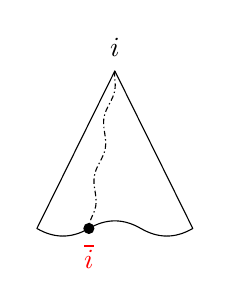
\begin{tikzpicture}[
edge from parent path=,
level distance=2cm,
level/.style={sibling distance=0.66cm/#1}
%,scale=1, every node/.style={transform shape}
]

  \tikzstyle{ref}=[circle,fill=black,inner sep=0.5mm]
  \tikzstyle{dashdot}=[dashed,dash pattern=on 2pt off 1pt on 0.5pt off 1pt]
  \tikzstyle{mysnake}=[decorate,decoration={snake,amplitude=0.4mm,segment length=0.75cm}]

  \node (c1) {}
    child { node (c2) {} }
    child { node (c3) [ref,label={below:$\overline{i}$}] {} }
    child { node (c4) {} }
    child { node (c5) {} };

  \node (c0) [minimum height=0.5cm,node distance=0.3cm,above of=c1] {$i$};

  \draw [join=round] (c1.center)
     to (c2.center) 
     to [bend right] (c3.center)
     to [bend left] (c4.center)
     to [bend right] (c5.center)
     -- cycle;

  \draw [mysnake,dashdot] (c1.center) -- (c3.center);

\end{tikzpicture}

  \end{center}
  \caption{Type 1 cut-point $i$ (reference within the same component)}
  \label{fig:t1cutpoint}
  \end{subfigure}
  \hfill
  \begin{subfigure}[b]{0.45\linewidth}
  \begin{center}
    
%%%%%%%%%%%%%%%%%%%%%%%%%%%%%%%%%%%%%%%%%%%%%%%%%%%%%%%%%%%%%%%%%%%%%%%
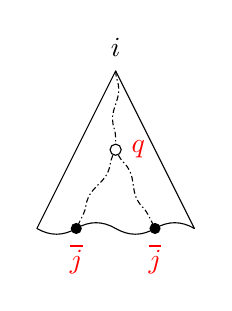
\begin{tikzpicture}[
edge from parent path=,
level distance=2cm,
level/.style={sibling distance=0.5cm/#1}
%,scale=1, every node/.style={transform shape}
]

  \tikzstyle{ref}=[circle,fill=black,inner sep=0.5mm]
  \tikzstyle{dashdot}=[dashed,dash pattern=on 2pt off 1pt on 0.5pt off 1pt]
  \tikzstyle{mysnake}=[decorate,decoration={snake,amplitude=0.4mm,segment length=0.75cm}]

  \node (c1) {}
    child { node (c2) {} }
    child { node (c3) [ref,label={below:$\overline{j}$}] {} }
    child { node (c4) {} }
    child { node (c5) [ref,label={below:$\overline{j}$}] {} }
    child { node (c6) {} };

  \node (c0) [minimum height=0.5cm,node distance=0.3cm,above of=c1] {$i$};

  \node (c7) [draw,circle,inner sep=0.5mm,node distance=1cm,below of=c1,label={right:$q$}] {};

  \draw [join=round] (c1.center)
     to (c2.center) 
     to [bend right] (c3.center)
     to [bend left] (c4.center)
     to [bend right] (c5.center)
     to [bend left] (c6.center)
     -- cycle;

  \draw [mysnake,dashdot] (c1.center) -- (c7);
  \draw [mysnake,dashdot] (c7) -- (c3.center);
  \draw [mysnake,dashdot] (c7) -- (c5.center);
  

\end{tikzpicture}

  \end{center}
  \caption{Type 2 cut-point $j$ (a single component contains
    multiple references to~$j$)}
  \label{fig:t2cutpoint}
  \end{subfigure}

  \noindent
  \begin{subfigure}[b]{0.45\linewidth}
  \begin{center}
    
%%%%%%%%%%%%%%%%%%%%%%%%%%%%%%%%%%%%%%%%%%%%%%%%%%%%%%%%%%%%%%%%%%%%%%%
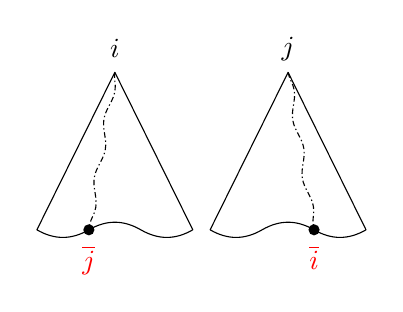
\begin{tikzpicture}[
edge from parent path=,
level distance=2cm,
level/.style={sibling distance=0.66cm/#1}
%,scale=1, every node/.style={transform shape}
]

  \tikzstyle{ref}=[circle,fill=black,inner sep=0.5mm]
  \tikzstyle{dashdot}=[dashed,dash pattern=on 2pt off 1pt on 0.5pt off 1pt]
  \tikzstyle{mysnake}=[decorate,decoration={snake,amplitude=0.4mm,segment length=0.75cm}]

  \node (c11) {}
    child { node (c12) {} }
    child { node (c13) [ref,label={below:$\overline{j}$}] {} }
    child { node (c14) {} }
    child { node (c15) {} };

  \node (c10) [minimum height=0.5cm,node distance=0.3cm,above of=c11] {$i$};

  \draw [join=round] (c11.center)
     to (c12.center) 
     to [bend right] (c13.center)
     to [bend left] (c14.center)
     to [bend right] (c15.center)
     -- cycle;

  \draw [mysnake,dashdot] (c11.center) -- (c13.center);

  \node (c21) [node distance=2.2cm,right of=c11] {}
    child { node (c22) {} }
    child { node (c23) {} }
    child { node (c24) [ref,label={below:$\overline{i}$}] {} }
    child { node (c25) {} };

  \node (c20) [minimum height=0.5cm,node distance=0.3cm,above of=c21] {$j$};

  \draw [join=round] (c21.center)
    to (c22.center) 
    to [bend right] (c23.center)
    to [bend left] (c24.center)
    to [bend right] (c25.center)
    -- cycle;

  \draw [mysnake,dashdot] (c21.center) -- (c24.center);

\end{tikzpicture}

  \end{center}
  \caption{Type 3 cut-points $i$ and $j$ (several mutually linked components)}
  \label{fig:t3cutpoint}
  \end{subfigure}
  \hfill
  \begin{subfigure}[b]{0.45\linewidth}
  \begin{center}
    
%%%%%%%%%%%%%%%%%%%%%%%%%%%%%%%%%%%%%%%%%%%%%%%%%%%%%%%%%%%%%%%%%%%%%%%
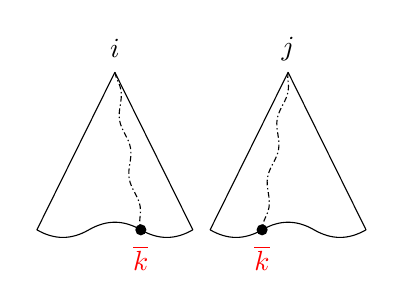
\begin{tikzpicture}[
edge from parent path=,
level distance=2cm,
level/.style={sibling distance=0.66cm/#1}
%,scale=1, every node/.style={transform shape}
]

  \tikzstyle{ref}=[circle,fill=black,inner sep=0.5mm]
  \tikzstyle{dashdot}=[dashed,dash pattern=on 2pt off 1pt on 0.5pt off 1pt]
  \tikzstyle{mysnake}=[decorate,decoration={snake,amplitude=0.4mm,segment length=0.75cm}]

  \node (c11) {}
    child { node (c12) {} }
    child { node (c13) {} }
    child { node (c14) [ref,label={below:$\overline{k}$}] {} }
    child { node (c15) {} };

  \node (c10) [minimum height=0.5cm,node distance=0.3cm,above of=c11] {$i$};

  \draw [join=round] (c11.center)
     to (c12.center) 
     to [bend right] (c13.center)
     to [bend left] (c14.center)
     to [bend right] (c15.center)
     -- cycle;

  \draw [mysnake,dashdot] (c11.center) -- (c14.center);

  \node (c21) [node distance=2.2cm,right of=c11] {}
    child { node (c22) {} }
    child { node (c23) [ref,label={below:$\overline{k}$}] {} }
    child { node (c24) {} }
    child { node (c25) {} };

  \node (c20) [minimum height=0.5cm,node distance=0.3cm,above of=c21] {$j$};

  \draw [join=round] (c21.center)
    to (c22.center) 
    to [bend right] (c23.center)
    to [bend left] (c24.center)
    to [bend right] (c25.center)
    -- cycle;

  \draw [mysnake,dashdot] (c21.center) -- (c23.center);

%  \node (c31) [node distance=2.2cm,right of=c21] {}
%    child { node (c32) {} }
%    child { node (c33) {} }
%    child { node (c34) {} }
%    child { node (c35) {} };

%  \node (c30) [minimum height=0.5cm,node distance=0.3cm,above of=c31] {$k$};

%  \draw [join=round] (c31.center)
%    to (c32.center) 
%    to [bend right] (c33.center)
%    to [bend left] (c34.center)
%    to [bend right] (c35.center)
%    -- cycle;

\end{tikzpicture}

  \end{center}
  \caption{Type 4 cut-point $k$ (referenced from several other components)}
  \label{fig:t4cutpoint}
  \end{subfigure}
  %
  % \centering
  % \begin{tabular}{cc}
  %   \parbox[t]{0.4\textwidth}{\centering
%%%%%%%%%%%%%%%%%%%%%%%%%%%%%%%%%%%%%%%%%%%%%%%%%%%%%%%%%%%%%%%%%%%%%%%
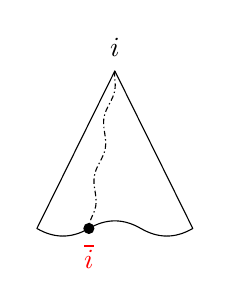
\begin{tikzpicture}[
edge from parent path=,
level distance=2cm,
level/.style={sibling distance=0.66cm/#1}
%,scale=1, every node/.style={transform shape}
]

  \tikzstyle{ref}=[circle,fill=black,inner sep=0.5mm]
  \tikzstyle{dashdot}=[dashed,dash pattern=on 2pt off 1pt on 0.5pt off 1pt]
  \tikzstyle{mysnake}=[decorate,decoration={snake,amplitude=0.4mm,segment length=0.75cm}]

  \node (c1) {}
    child { node (c2) {} }
    child { node (c3) [ref,label={below:$\overline{i}$}] {} }
    child { node (c4) {} }
    child { node (c5) {} };

  \node (c0) [minimum height=0.5cm,node distance=0.3cm,above of=c1] {$i$};

  \draw [join=round] (c1.center)
     to (c2.center) 
     to [bend right] (c3.center)
     to [bend left] (c4.center)
     to [bend right] (c5.center)
     -- cycle;

  \draw [mysnake,dashdot] (c1.center) -- (c3.center);

\end{tikzpicture}
}&
  %   \parbox[t]{0.4\textwidth}{\centering
%%%%%%%%%%%%%%%%%%%%%%%%%%%%%%%%%%%%%%%%%%%%%%%%%%%%%%%%%%%%%%%%%%%%%%%
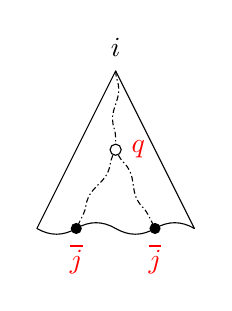
\begin{tikzpicture}[
edge from parent path=,
level distance=2cm,
level/.style={sibling distance=0.5cm/#1}
%,scale=1, every node/.style={transform shape}
]

  \tikzstyle{ref}=[circle,fill=black,inner sep=0.5mm]
  \tikzstyle{dashdot}=[dashed,dash pattern=on 2pt off 1pt on 0.5pt off 1pt]
  \tikzstyle{mysnake}=[decorate,decoration={snake,amplitude=0.4mm,segment length=0.75cm}]

  \node (c1) {}
    child { node (c2) {} }
    child { node (c3) [ref,label={below:$\overline{j}$}] {} }
    child { node (c4) {} }
    child { node (c5) [ref,label={below:$\overline{j}$}] {} }
    child { node (c6) {} };

  \node (c0) [minimum height=0.5cm,node distance=0.3cm,above of=c1] {$i$};

  \node (c7) [draw,circle,inner sep=0.5mm,node distance=1cm,below of=c1,label={right:$q$}] {};

  \draw [join=round] (c1.center)
     to (c2.center) 
     to [bend right] (c3.center)
     to [bend left] (c4.center)
     to [bend right] (c5.center)
     to [bend left] (c6.center)
     -- cycle;

  \draw [mysnake,dashdot] (c1.center) -- (c7);
  \draw [mysnake,dashdot] (c7) -- (c3.center);
  \draw [mysnake,dashdot] (c7) -- (c5.center);
  

\end{tikzpicture}
}\\
  %   (a) & (b) \\
  %   \parbox[t]{0.4\textwidth}{\centering
%%%%%%%%%%%%%%%%%%%%%%%%%%%%%%%%%%%%%%%%%%%%%%%%%%%%%%%%%%%%%%%%%%%%%%%
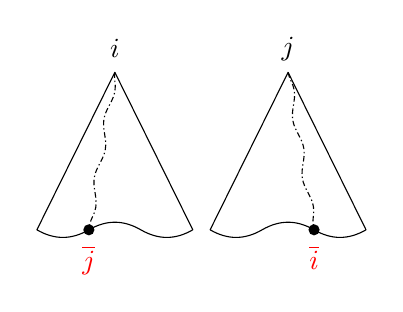
\begin{tikzpicture}[
edge from parent path=,
level distance=2cm,
level/.style={sibling distance=0.66cm/#1}
%,scale=1, every node/.style={transform shape}
]

  \tikzstyle{ref}=[circle,fill=black,inner sep=0.5mm]
  \tikzstyle{dashdot}=[dashed,dash pattern=on 2pt off 1pt on 0.5pt off 1pt]
  \tikzstyle{mysnake}=[decorate,decoration={snake,amplitude=0.4mm,segment length=0.75cm}]

  \node (c11) {}
    child { node (c12) {} }
    child { node (c13) [ref,label={below:$\overline{j}$}] {} }
    child { node (c14) {} }
    child { node (c15) {} };

  \node (c10) [minimum height=0.5cm,node distance=0.3cm,above of=c11] {$i$};

  \draw [join=round] (c11.center)
     to (c12.center) 
     to [bend right] (c13.center)
     to [bend left] (c14.center)
     to [bend right] (c15.center)
     -- cycle;

  \draw [mysnake,dashdot] (c11.center) -- (c13.center);

  \node (c21) [node distance=2.2cm,right of=c11] {}
    child { node (c22) {} }
    child { node (c23) {} }
    child { node (c24) [ref,label={below:$\overline{i}$}] {} }
    child { node (c25) {} };

  \node (c20) [minimum height=0.5cm,node distance=0.3cm,above of=c21] {$j$};

  \draw [join=round] (c21.center)
    to (c22.center) 
    to [bend right] (c23.center)
    to [bend left] (c24.center)
    to [bend right] (c25.center)
    -- cycle;

  \draw [mysnake,dashdot] (c21.center) -- (c24.center);

\end{tikzpicture}
}&
  %   \parbox[t]{0.4\textwidth}{\centering
%%%%%%%%%%%%%%%%%%%%%%%%%%%%%%%%%%%%%%%%%%%%%%%%%%%%%%%%%%%%%%%%%%%%%%%
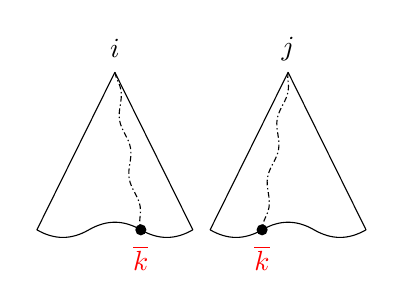
\begin{tikzpicture}[
edge from parent path=,
level distance=2cm,
level/.style={sibling distance=0.66cm/#1}
%,scale=1, every node/.style={transform shape}
]

  \tikzstyle{ref}=[circle,fill=black,inner sep=0.5mm]
  \tikzstyle{dashdot}=[dashed,dash pattern=on 2pt off 1pt on 0.5pt off 1pt]
  \tikzstyle{mysnake}=[decorate,decoration={snake,amplitude=0.4mm,segment length=0.75cm}]

  \node (c11) {}
    child { node (c12) {} }
    child { node (c13) {} }
    child { node (c14) [ref,label={below:$\overline{k}$}] {} }
    child { node (c15) {} };

  \node (c10) [minimum height=0.5cm,node distance=0.3cm,above of=c11] {$i$};

  \draw [join=round] (c11.center)
     to (c12.center) 
     to [bend right] (c13.center)
     to [bend left] (c14.center)
     to [bend right] (c15.center)
     -- cycle;

  \draw [mysnake,dashdot] (c11.center) -- (c14.center);

  \node (c21) [node distance=2.2cm,right of=c11] {}
    child { node (c22) {} }
    child { node (c23) [ref,label={below:$\overline{k}$}] {} }
    child { node (c24) {} }
    child { node (c25) {} };

  \node (c20) [minimum height=0.5cm,node distance=0.3cm,above of=c21] {$j$};

  \draw [join=round] (c21.center)
    to (c22.center) 
    to [bend right] (c23.center)
    to [bend left] (c24.center)
    to [bend right] (c25.center)
    -- cycle;

  \draw [mysnake,dashdot] (c21.center) -- (c23.center);

%  \node (c31) [node distance=2.2cm,right of=c21] {}
%    child { node (c32) {} }
%    child { node (c33) {} }
%    child { node (c34) {} }
%    child { node (c35) {} };

%  \node (c30) [minimum height=0.5cm,node distance=0.3cm,above of=c31] {$k$};

%  \draw [join=round] (c31.center)
%    to (c32.center) 
%    to [bend right] (c33.center)
%    to [bend left] (c34.center)
%    to [bend right] (c35.center)
%    -- cycle;

\end{tikzpicture}
}\\
  %   (c) & (d)
  % \end{tabular}
  %

  \caption{Four possible types of cut-points.}
  % (a) A Type~1 cut-point appearing as
  % a~reference in the same component whose root it is. (b) A single component containing
  % multiple references to a Type~2 cut-point. (c) Two components mutually linked via Type~3
  % cut-points. (d) A Type~4 cut-point being referred from two other components
  % simultaneously.}

  \label{fig:cptypes}

\end{figure}

We are now going to describe four types of cut-points (illustrated in
Fig.~\ref{fig:cptypes}), each of which is eliminated by a special algorithm. 
We distinguish whether a~node is a cut-point due to a cycle in the heap or whether it is only referenced multiple times, 
and we also distinguish whether this can be seen locally within a single component or only across several different components.
This gives us four different types of cut-points.
One cut-point can be of multiple types.

In particular, Type~1 cut-points arise, for instance, when one works with cyclic
lists. In such a case, a single TA component encodes a set of cyclic lists with the
cycle encoded using a leaf that refers back to the root of the component. Type~2
cut-points are those cut-points that are referenced multiple times from within
a~single component. These typically arise when one deals with trees whose all leaves
refer to some designated node (e.g., the root). Next, a set of two or more cut-points
is said to consist of cut-points of Type~3 if the components rooted at them are linked
in a~cycle. A typical scenario where such cut-points appear is working with
doubly-linked lists, where the cycle appears between a~pair of successive list nodes.
Observe that each inner element of the lists is pointed from its predecessor and
from its successor at the same time, and so (without using a hierarchical encoding)
every element has to reside in its own component (and the present loops cannot be
reduced to loops within a single component with a cut-point of Type~1). Finally,
Type~4 cut-points are the cut-points referred from two or more components at the
same time.

In the following section, we will show how to eliminate cut-points of Type~1 and 2
as well as some cut-points of Type~3. In the case of Type~3 cut-points, 
we only show how to deal with pairs of cut-points of Type~3 that are the roots of neighboring components linked
in a~cyclic way.
We do not consider any other form of Type~3 cut-points since we have not
encountered them in any of our case studies (in particular, we have not
encountered loops going through more than two cut-points).
We also do not have any direct elimination procedure for cut-points of Type~4.
This was not needed in our case studies either, because no matter how
ubiquitous cut-points of Type~4 were, they were always of other types too, and
eliminating cut-points of Type~1, 2, and~3 either eliminated Type~4 too or
turned Type~4 cut-points to one of the first three types.
For instance, in the case of doubly-linked lists, each node in fact
corresponds to a cut-point of Type~3 and Type~4 at the same time. Nevertheless, when
we fold the parts of the heap that make the concerned nodes to be cut-points of
Type~3, there will not remain any cut-points of Type~4 either (see
Fig.~\ref{fig:dllelim} for an illustration). 

\begin{figure}[t]
  \centering
    \parbox{0.7\textwidth}{\centering
%%%%%%%%%%%%%%%%%%%%%%%%%%%%%%%%%%%%%%%%%%%%%%%%%%%%%%%%%%%%%%%%%%%%%%%
\begin{tikzpicture}[
node distance=1.8cm,
>=stealth',
bend angle=45,
auto,
level distance=1.2cm,
level 1/.style={sibling distance=1cm},
level 2/.style={sibling distance=0.7cm},
level 3/.style={sibling distance=0.4cm},
edge from parent path=,
shorten >=1pt,
shorten <=0.5pt,
%thin,
%->,
scale=0.9,
every node/.style={transform shape}
]

  \tikzstyle{cell}=[circle,thick,draw=black,minimum size=5mm,inner sep=0pt]
  \tikzstyle{mylabel}=[sloped,inner sep=2pt]
  \tikzstyle{mypoint}=[inner sep=0pt,outer sep=0pt,midway]
  \tikzstyle{red cell}=[circle,draw=red!75,fill=red!20,minimum size=5mm,inner sep=0pt]

%  \tikzstyle{every label}=[red]

  \begin{scope}%[mylabel/.style={scale=0.8}]%[every label/.style={scale=0.8}]
	
    % First net
    \node [red cell,label={above:\figtext{$i$}}] (c1) {}
		child { node [cell,red,label={below:\figtext{$\overline{i-1}$}}] (c11) {} }
		child { node [cell,red,label={[red]below:\figtext{$\overline{i+1}$}}] (c12) {} };
    \node [red cell,label={[red] above:\figtext{$i+1$}},right=of c1] (c2) {}
		child { node [cell,red,label={below:\figtext{$\overline{i}$}}] (c21) {} }
		child { node [cell,red,label={below:\figtext{$\overline{i+2}$}}] (c22) {} };

    \node [red cell,label={above:\figtext{$i+2$}},right=of c2] (c3) {}
		child { node [cell,red,label={[red]below:\figtext{$\overline{i+1}$}}] (c31) {} }
		child { node [cell,red,label={below:\figtext{$\overline{i+3}$}}] (c32) {} };

	\path 
		(c1) edge [->,inner sep=0pt] node [mypoint,outer sep=-0.5pt,label={[mylabel]
    above right:\figtext{next}}] (p2) {} (c12)
		(c1) edge [swap,->,inner sep=0pt] node [mypoint,outer
    sep=-0.5pt,label={[mylabel] above left:\figtext{prev}}] (p1) {} (c11)
		(c2) edge [->,inner sep=0pt] node [mypoint,outer sep=-0.5pt,label={[mylabel]
    above right:\figtext{next}}] (p4) {} (c22)
		(c2) edge [swap,->,inner sep=0pt] node [mypoint,outer
    sep=-0.5pt,label={[mylabel] above left:\figtext{prev}}] (p3) {} (c21)
		(c3) edge [->,inner sep=0pt] node [mypoint,label={[mylabel] above right:\figtext{next}}] (p6) {} (c32)
		(c3) edge [swap,->,inner sep=0pt] node [mypoint,label={[mylabel] above left:\figtext{prev}}] (p5) {} (c31)
    ;

	\node [node distance=1.3cm,left=of c1.south,label={below:\figtext{$\dots$}}] {};
	\node [node distance=1.3cm,right=of c3.south,label={below:\figtext{$\dots$}}] {};

	\node [dashed,draw=black!50,fit=(c1.north east) (c12) (c21) (c2.north west),rounded corners=4pt,inner sep=2pt] {};

	\node [dashed,draw=black!50,fit=(c2.north east) (c22) (c31) (c3.north west),rounded corners=4pt,inner sep=2pt] {};

	\draw
		(p2.center) to[out=-135,in=-45] (p1.center)
		(p4.center) to[out=-135,in=-45] (p3.center)
		(p6.center) to[out=-135,in=-45] (p5.center)
	;

  \end{scope}

\end{tikzpicture}
}

    $\Downarrow$

    \parbox{0.7\textwidth}{\centering
%%%%%%%%%%%%%%%%%%%%%%%%%%%%%%%%%%%%%%%%%%%%%%%%%%%%%%%%%%%%%%%%%%%%%%%
\begin{tikzpicture}[
node distance=1.8cm,
>=stealth',
bend angle=45,
auto,
level distance=1.2cm,
level 1/.style={sibling distance=1cm},
level 2/.style={sibling distance=0.7cm},
level 3/.style={sibling distance=0.4cm},
edge from parent path=,
shorten >=1pt,
shorten <=0.5pt,
%thin,
%->,
scale=0.9,
every node/.style={transform shape}
]

  \tikzstyle{cell}=[circle,thick,draw=black,minimum size=5mm,inner sep=0pt]
  \tikzstyle{red cell}=[circle,draw=red!75,fill=red!20,minimum size=5mm,inner sep=0pt]

%  \tikzstyle{every label}=[red]

  \begin{scope}%[mylabel/.style={scale=0.8}]%[every label/.style={scale=0.8}]
	
    % First net
    \node [red cell,label={above:\figtext{$i$}}] (c1) {}
%		child { node [cell,red,label={[red]below:\figtext{$i-1$}}] (c11) {} }
		child { node [cell,red,label={below:\figtext{$\overline{i+1}$}}] (c12) {} };
    \node [red cell,label={above:\figtext{$i+1$}},right=of c1] (c2) {}
%		child { node [cell,red,label={[red]below:\figtext{$i$}}] (c21) {} }
		child { node [cell,red,label={below:\figtext{$\overline{i+2}$}}] (c22) {} };

    \node [red cell,label={above:\figtext{$i+2$}},right=of c2] (c3) {}
%		child { node [cell,red,label={[red]below:\figtext{$i+1$}}] (c31) {} }
		child { node [cell,red,label={below:\figtext{$\overline{i+3}$}}] (c32) {} };

	\path 
		(c1) edge [->] node [inner sep=3pt] {\figtext{DLL}} (c12)
		(c2) edge [->] node [inner sep=3pt] {\figtext{DLL}} (c22)
		(c3) edge [->] node [inner sep=3pt] {\figtext{DLL}} (c32)
    ;

	\node [node distance=1.3cm,left=of c1.south,label={below:\figtext{$\dots$}}] {};
	\node [node distance=1.3cm,right=of c3.south,label={below:\figtext{$\dots$}}] {};

  \end{scope}

\end{tikzpicture}
}

  \caption{Folding of a doubly-linked list with a Type~4 cut-point~$i+1$}
  %highlighted in red}
  \label{fig:dllelim}
\end{figure}

% \ol{HIDDEN}
% We are now going to describe 4 possible types of cut-points (see Figure~\ref{fig:cptypes})
% which can appear in various combinations (e.g., a single cut-point can be of Type~1 and of
% Type~2 at the same time). Type~1 cut-points arise when one works, for instance, with cyclic
% lists. In such cases, a single tree component represents the contents of entire lists up to
% the last link which closes the cycle (the cycle is represented using a reference back to the
% root of the component itself). Type~2 cut-points are those cut-points which are referred
% multiple times from within a single component. These typically arise when one deals with
% a~set of trees in which every tree contains references to some designated node in its leaves
% (e.g., a reference to its root). Two cut-points whose corresponding components mutually
% refer to each other are called cut-points of Type~3. Such cut-points usually appear when
% one works with doubly-linked lists where they correspond to a pair of successive list
% nodes. Observe, that each inner element of the lists is pointed from its predecessor and
% from its successor at the same time, therefore every element has to initially reside
% in its own component. Finally, Type~4 cut-points are the cut-points referred from
% 2 or more components at the same time. 

% The 4 types follow from the way cut-points may arise. Namely, a~cut-point arises when there
% is a~loop in the heap or some node is referenced multiple times. Both of these scenarios
% can then happen within a single component or across several different components. If a~loop
% goes through more than 2 roots and all these roots correspond to cut-points, which are not
% suitable for elimination via another folding, then the cut-points within the loop cannot
% be eliminated. The same applies to a~cut-point referenced from multiple components. We have
% not encountered loops going through more than 2 cut-points in the considered examples. On
% the other hand, cut-points referenced from multiple components are quite ubiquitous. They,
% however, always appeared in combination with other types of cut-points in our experiments.
% In particular case of a doubly-linked list, each node corresponds to a~cut-point of Type~3
% and Type~4 at the same time. Nevertheless, after performing Type~3 elimination the Type~4
% cut-points also disappear (see Figure~\ref{fig:dllelim} for an illustration).


%*******************************************************************************
\subsection{Cut-point Elimination}
\label{ref:cpelim}
%*******************************************************************************

In this section, we discuss the automatic elimination of cut-points of Type~1, 2, and 3, discussed
in the previous section.
As we have already mentioned, it might happen that some cut-point is of more than one
type, which is solved by several applications of the folding algorithm. The heuristic,
which currently seems to give the best results in our experiments, eliminates cut-points
in the order 3, 2, and 1.
%\comment[ol]{actually, this is contrary to our CAV'13 algorithm, which goes from smallest
%knots to larger knots}

{
Before we explain how to deal with the particular types of cut-points, we introduce the so-called \emph{component slicing}.
%
On the level of a single forest $\tuple{t_1,\ldots,t_n,\sigma}$, 
folding is an operation that
(1)~selects the part of the forest to be folded into the new box, in the form of 
one root component~$t_i$, a set of selectors~$S$, and possibly several
additional components, and 
(2)~\emph{slices} the component $t_i$ into two parts, the \emph{kernel} and the
\emph{residue}.
The kernel is the root and its sub-trees connected to it by the selectors of~$S$. 
The residue is the root and its sub-trees connected to it by the remaining
selectors outside~$S$.
The box will then hide the kernel and the eventual additional components.
The original forest is then represented by its modification in which (i)~$t_i$~is replaced by a component created from the residue
by adding an additional hyperedge leading from the root labeled by the new box, and (ii)~the additional components are removed.

%We, however,
%perform folding not on a~single graph, but on a~set of graphs represented by
%some FA $\fa = \tuple{\tas, \asgn}$. Therefore, whenever we want to perform folding
%of some part of a component $\ta_i$ (or, in general, several components) into a box $B$,
%we need to proceed as follows. First, we identify a transition $t$ of $\ta_i$ at which we
%want to perform the folding (or, we identify a transition in each component
%in which the folding should occur at the same time), and we decide which part of $t$ will
%be hidden inside the (not yet known) box~$B$. This way, we choose which sub-graphs will
%be hidden---in particular, we will hide the selected part of the transition and everything
%that is (top-down) reachable from that part of the transition in~$\ta_i$.

We will now discuss how slicing is implemented on the level of forest automata.
Let us recall that an FA is a~tuple $\fa = \tuple{A_i \cdots A_n,\sigma}$ where the TAs~$A_i$, for $1\leq i \leq n$,
have transitions of the form $\transover q {a_1\cdots a_n} {q_1,\ldots, q_n}$. 
Such transition generates a tree node $v$ connected to nodes $v_1,\ldots,v_n$ via edges $(n,a_i,n_i)$ for each $i:1\leq i \leq n$.   
The symbols $a_i$ are either selectors or indexed boxes of the form $B_{(k)}$, where $B$ is a box and $1\leq k \leq \rankof B$, where the symbols $B_{(1)},\ldots,B_{(\rankof B)}$ always appear together and represent a hyperedge labeled by $B$.
%
We use additional technical assumptions on the form of FAs that simplify the
operation of slicing; in the symbolic execution, we always keep FAs in the form.
%
Namely, (1)~root states of tree automata components never appear as child
states of transitions,
(2)~for every state, all transitions with the state as the parent state have
the same vector of symbols
(both can be achieved by simple automata transformations).
%
Slicing will be further specified using the operator $\cut$ called
\emph{transition cut} that, when given a~transition $t =  q \rightarrow
a_1\cdots a_n (q_1,\dots,q_n)$ and a~set of selectors and indexed boxes~$E$,
produces a~new transition~$t \cut E$ that is made from~$t$ by, for all~$a_i \in
E$, erasing~$a_i$ from the sequence of symbols $a_1 \cdots a_n$ and also
erasing $q_i$ from the sequence of states $q_1,\ldots,q_n$.
%
Slicing of the $i$-th component~$A_i$ of~$F$ w.r.t.\ a~set of selectors or
indexed boxes~$E$ then produces two versions of~$A_i$, again called the kernel
and the residue.
The residue has each accepting transition $t = \transover {q}
{a_1\cdots a_m} {q_1,\ldots,q_m}$ of $A_i$ replaced by $t\cut E$, while the
residue has the accepting transition replaced by $t\cut
\{a_1,\ldots,a_k\}\setminus E$ (see Fig.~\ref{fig:slicing} for an illustration
of slicing).
 

%In order to obtain the box~$B$, we split $t$ into two new transitions $t_k$ and~$t_r$ such that
%$t_k$ is the part of $t$ to be put into $B$ and $t_r$ contains the part of~$t$ not
%contained in~$t_k$.
%Furthermore, we create two new components (automata) called the \emph{kernel}
%and the \emph{residue}. The kernel contains~$t_k$ as an accepting transition (i.e.,
%a~transition with an accepting state as its parent state) together with all other
%transitions (top-down) reachable from~$t_k$ within~$\ta_i$. As~a~result, the kernel
%defines what~$B$ is. The residue is obtained by replacing~$t$ by~$t_r$ in~$\ta_i$. If we
%now directly replaced~$\ta_i$ by the residue in~$\fa$, we would obtain a set of graphs
%in which the selected sub-graphs were entirely removed. To simulate the replacement of the
%part of the graph by the hyperedge, we append~$B$ to~$t_r$ inside the residue. The
%process of splitting a~selected component into kernel and residue is called
%component slicing (see Fig.~\ref{fig:slicing} for an illustration of this
%concept).

\begin{figure}[t]
  \centering
  \begin{tabular}{cccc}
    && \textbf{kernel} & \textbf{residue}\\
    \parbox{0.35\textwidth}{\centering
%%%%%%%%%%%%%%%%%%%%%%%%%%%%%%%%%%%%%%%%%%%%%%%%%%%%%%%%%%%%%%%%%%%%%%%
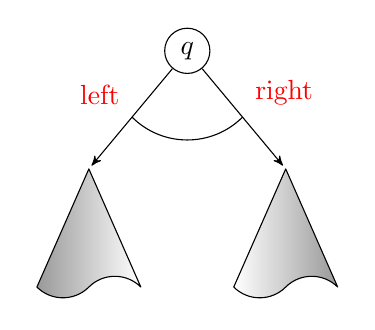
\begin{tikzpicture}[
%edge from parent path=,
level distance=1.5cm,
level 1/.style={sibling distance=2.5cm},
level 2/.style={sibling distance=0.66cm},
every node/.style={transform shape},
edge from parent path=,
>=stealth',
,bend angle=45,
auto
%,scale=1, every node/.style={transform shape}
]

  \tikzstyle{cell}=[draw=black,circle,minimum size=4.5mm,inner sep=0.3em]
  \tikzstyle{mysnake}=[decorate,decoration={snake,amplitude=0.4mm,segment length=0.75cm}]

  \node (c1) [cell] {$q$}
    child { node [inner sep=1pt] (c11) {} 
		child { node (c111) {} }
		child { node (c112) {} }
		child { node (c113) {} }
	}
    child { node [inner sep=1pt] (c12) {} 
		child { node (c121) {} }
		child { node (c122) {} }
		child { node (c123) {} }
	};

	\path (c1) edge [swap,->,inner sep=1pt] node (f1) [midway,label={[sloped,inner
  sep=2pt]above left:left}] {} (c11);
	\path (c1) edge [->,inner sep=1pt] node (f2) [midway,label={[sloped,inner
  sep=2pt]above right:right}] {} (c12);

	\draw [join=round] (c11.center) -- (c111.center) to [bend right] (c112.center) to [bend left] (c113.center) -- cycle;
	\draw [join=round] (c12.center) -- (c121.center) to [bend right] (c122.center) to [bend left] (c123.center) -- cycle;

	\draw [black] (f1) to[out=-45,in=-135] node [midway,inner sep=5pt] {} (f2);

	\begin{pgfonlayer}{background}
	\path [right color=white,left color=black!40,shading=axis]
		(c11.center) -- (c111.center) to [bend right] (c112.center) to [bend left]	(c113.center) -- cycle;
	\path [left color=white,right color=black!40,shading=axis]
		(c12.center) -- (c121.center) to [bend right] (c122.center) to [bend left]	(c123.center) -- cycle;
	\end{pgfonlayer}

\end{tikzpicture}
} &
    $\Rightarrow$ &
    \parbox{0.2\textwidth}{\centering
%%%%%%%%%%%%%%%%%%%%%%%%%%%%%%%%%%%%%%%%%%%%%%%%%%%%%%%%%%%%%%%%%%%%%%%
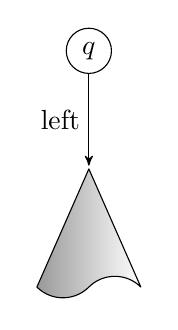
\begin{tikzpicture}[
%edge from parent path=,
level distance=1.5cm,
level 1/.style={sibling distance=2.5cm},
level 2/.style={sibling distance=0.66cm},
every node/.style={transform shape},
edge from parent path=,
>=stealth',
,bend angle=45,
auto
%,scale=1, every node/.style={transform shape}
]

  \tikzstyle{cell}=[draw=black,circle,minimum size=4.5mm,inner sep=0.3em]
  \tikzstyle{mysnake}=[decorate,decoration={snake,amplitude=0.4mm,segment length=0.75cm}]

  \node (c1) [cell] {$q$}
    child { node [inner sep=1pt] (c11) {} 
		child { node (c111) {} }
		child { node (c112) {} }
		child { node (c113) {} }
	};

	\path (c1) edge [swap,->,inner sep=3pt] node [midway] {\figtext{left}} (c11);

	\draw [join=round] (c11.center) -- (c111.center) to [bend right] (c112.center) to [bend left] (c113.center) -- cycle;

	\begin{pgfonlayer}{background}
	\path [right color=white,left color=black!40,shading=axis]
		(c11.center) -- (c111.center) to [bend right] (c112.center) to [bend left]	(c113.center) -- cycle;
	\end{pgfonlayer}

\end{tikzpicture}
} &
    \parbox{0.2\textwidth}{\centering
%%%%%%%%%%%%%%%%%%%%%%%%%%%%%%%%%%%%%%%%%%%%%%%%%%%%%%%%%%%%%%%%%%%%%%%
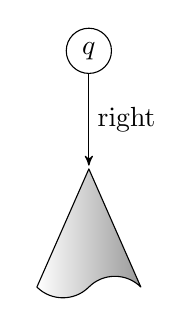
\begin{tikzpicture}[
%edge from parent path=,
level distance=1.5cm,
level 1/.style={sibling distance=2.5cm},
level 2/.style={sibling distance=0.66cm},
every node/.style={transform shape},
edge from parent path=,
>=stealth',
,bend angle=45,
auto
%,scale=1, every node/.style={transform shape}
]

  \tikzstyle{cell}=[draw=black,circle,minimum size=4.5mm,inner sep=0.3em]
  \tikzstyle{mysnake}=[decorate,decoration={snake,amplitude=0.4mm,segment length=0.75cm}]

  \node (c2) [cell] {$q$}
    child { node [inner sep=1pt] (c22) {} 
		child { node (c221) {} }
		child { node (c222) {} }
		child { node (c223) {} }
	};

	\path (c2) edge [->,inner sep=3pt] node [midway] {\figtext{right}} (c22);

	\draw [join=round] (c22.center) -- (c221.center) to [bend right] (c222.center) to [bend left] (c223.center) -- cycle;

	\begin{pgfonlayer}{background}
	\path [left color=white,right color=black!40,shading=axis]
		(c22.center) -- (c221.center) to [bend right] (c222.center) to [bend left]	(c223.center) -- cycle;
	\end{pgfonlayer}

\end{tikzpicture}
}
  \end{tabular}

  \caption{An example of component slicing. The left part shows the original
  automaton
  that is to be sliced at the state $q$ according to the edge labeled by ``left'' (i.e.,
  we perform
  $\transover q {\langle \mathit{left},\mathit{right} \rangle} {q_1,q_2} \cut \{\mathit{left}\}$).
  % $(\langle \mathit{left},\mathit{right} \rangle (q_1,q_2) \rightarrow q) \cut \{\mathit{left}\}$).
  The
  right part shows the result after slicing, in which the kernel contains the structure
  reachable via ``left'', and the residue contains the rest of the original automaton
  (in this case, the structure reachable via ``right'').}

  \label{fig:slicing}

\end{figure}

%% \ol{say something about nullary boxes (i.e., they can be represented by a unary
%% box to some fake location}
%% 
%% \ol{say that when cutting transitions, if we cut a box-selector, then all
%% selectors of the box need to be cut}
%% 
%% In order to give a formal description of the operator $\cut$, we need to introduce
%% several auxiliary operations. In particular, let $t_1 = (q_1,\dots,q_n)$ and
%% $t_2=(r_1,\dots,r_m)$ be two tuples (of states). We define the concatenation
%% of~$t_1$ and~$t_2$, denoted by $t_1 \circ t_2$ as the $(n+m)$ tuple
%% $(q_1,\dots,q_n,r_1,\dots,r_m)$.
%% We also define a tuple selection operation, denoted by $t_1[i,k]$, which produces the
%% $k$-tuple $(q_i,\dots,q_{i+k-1})$ provided that $1 \leq i \leq n$ and $i+k-1 \leq n$.
%% To summarize:
%% 
%% $$
%% \begin{array}{lcl}
%%   (q_1,\dots,q_n) \circ (r_1,\dots,r_m) & = & (q_1,\dots,q_n,r_1,\dots,r_m)\\
%%   (q_1,\dots,q_n)[i,k] & = & (q_i,\dots,q_{i+k-1})\textrm{.}\\
%% \end{array}
%% $$
%% 
%% We aim at breaking a transition $t = \transover q {a_1\dots a_m}{q_1,\dots,q_m}$
%% into pieces composed of $a_i$ and the child states connected to~$a_i$.
%% Therefore, we further define
%% a~function called $\pickof{ \transover q {a_1\dots a_m}{q_1,\dots,q_m}}{i}$, which selects the tuple
%% of child states corresponding to~$a_i$ from the transition
%% $\transover q {a_1\dots a_m}{q_1,\dots,q_m}$ (provided $1 \leq i \leq m$ and
%% $\#_v(a_1\dots a_n) = m$):
%% \ol{OJ! OJ! OJ! this whole part needs to be unfucked!!}
%% %
%% \[
%%   \pickof{\transover q {a_1\dots a_n}{q_1,\dots,q_m}}{i} = (q_1,\dots,q_m)[\#_v(a_1\dots a_{i-1}) + 1, \#_e(a_i)]\textrm{.}
%% \]
%% %
%% \comment[ol]{what is $\#_e$?}
%% Using the previous definition, we define a function called $\splitting$, which splits
%% a~transition into a tuple of pairs containing parts of the original symbol and the connected
%% tuples of child states:
%% \[
%% \splitting(t = \transover q {a_1\dots a_n}{q_1,\dots,q_m}) = ((a_1,\pickof t
%% 1),\dots,(a_n,\pickof t n))\textrm{.}
%% \]
%% In order to transform a tuple containing separated parts of the symbol and corresponding
%% tuples of states into a transition, we define a complementary function to
%% $\splitting$ called
%% $\joinfun$, which, given a tuple of pairs of the above form and a state, creates a new
%% transition as follows ($(\mathbf{s_1}\dots\mathbf{s_n})$ denotes the concatenation of tuples
%% $\mathbf{s_1}\circ\mathbf{s_2}\circ\dots\circ\mathbf{s_n}$):
%% %
%% $$
%% \joinfun(((a_1,\mathbf{s_1}),\dots,(a_n,\mathbf{s_n})), q) = \transover q
%% {a_1\dots a_n}{\mathbf{s_1}\dots\mathbf{s_n}}
%% $$
%% %
%% At this point, we are able to split a transition into pieces and then join these pieces back
%% together. We, however, do not intend to join all of the original pieces but only some subset
%% of them. Therefore, we also define a filtering function $\filter{f}$, which
%% removes certain elements (determined by the Boolean function~$f$) of the tuple it
%% receives as the input:
%% \[
%% \begin{array}{lcl}
%%   \filter{f} () & = & ()\\
%%   \filter{f} (x_1,\dots,x_n) & = & \left\{
%%   \begin{array}{cl}
%%     (x_1) \cdot \filter{f} (x_2,\dots,x_n) & \textrm{if } f(x_1) \\
%%     \filter{f} (x_2,\dots,x_n) & \textrm{otherwise}
%%   \end{array}\right.
%% \end{array}
%% \]
%% Finally, we are ready to give the definition of the operator $t \cut E$, which first splits
%% the given transition $t$, then it keeps only those pairs containing elements of the set $E$,
%% and, in the last step, it joins the remaining pairs into a new transition:
%% \[
%% (t = \trans q {q_1,\dots,q_n}) \cut E = \joinfun(\filter{f}
%% (\splitting(t)), q)
%% \]
%% where $f((a,\mathbf{s})) \iff a \in E$.

%Now, for a given state $q$, a fixed symbol $\edgesymb = a_1\dots a_n$, and a~given set of
%selectors (or boxes) $E \subseteq \{a_1,\dots,a_n\}$, slicing of a component TA works as
%follows. We first create a kernel and a residue as two separate copies of the component
%to be sliced. Then, in the kernel, we replace each transition~$t$ of the form
%$\trans q {q_1,\dots,q_m}$ by the transition~$t \cut E$. Contrary to that,
%we replace each transition~$t$ of the form $\trans q {q_1,\dots,q_m}$ by the
%transition $t \cut (\{a_1,\dots,a_n\}\setminus E)$ in the residue.
%
%Note that all steps within our symbolic execution produce automata in which all
%transitions of the form $\trans q {\,\dots\,}$ are labeled by the same
%symbol~$\edgesymb$ (i.e., $\{\trans q {\,\dots\,}, \transover q
%{\edgesymb'}{\,\dots\,}\} \subseteq \Delta \Rightarrow \edgesymb = \edgesymb'$).
%Moreover, the abstraction never
%collapses states~$q_1$ and~$q_2$ if there exist transitions $\trans {q_1}
%{\,\dots\,}$ and
%$\transover {q_2} {\edgesymb'}{\,\dots\,}$ such that $\edgesymb \neq \edgesymb'$
%(see \secref{sec:abstraction}).
%Hence, we assume that the symbol is always specified implicitly by the
%state~$q$, and, therefore, in the following, the component slicing is
%parameterized by a state and a set of selectors (of boxes) only.


%--------------------------------------------
\subsubsection*{Type~1 Cut-point Elimination}
%\paragraph{Type~1.}

A Type~1 cut-point (cf.\ Fig.~\ref{fig:t1cutpoint}) corresponds to a component
that
contains references to its own root (these are called \emph{self-references} in the following).
To eliminate such a~cut-point, we want to ``hide'' all the self-references into a~box.
Therefore, we identify a~set $E$ of all selectors (or boxes) within the accepting
transitions that lie on some path going to some self-reference. 
%(for this, we
%conveniently use labels introduced in \secref{sec:facan} \comment[ol]{ha! no
%fucking labels in this text!}). 
Then, we perform
slicing of the component w.r.t.\
%parametrized by the appropriate accepting state and 
the set~$E$ to obtain the kernel containing all self-references and
a~residue containing the rest.
Suppose that the root references appearing in the kernel form the set $R
\subseteq \{1,\dots,n\}$; the rank of the new box will be $k = |R|-1$.

Next, we perform a~depth-first traversal on the kernel and we rename all
references from~$R$ according to the
order in which they are visited (such that the self-references are always
relabeled to $0$) to obtain a mapping $f : R \rightarrow \{0,\dots,k\}$.
The relabeled kernel
is transformed into a~new box~$\botox$ with $\rankof \botox = k$.
All accepting transitions
$\trans q {q_1,\dots,q_n}$ of the residue are modified to
%
$$
\transover q {\edgesymb B_{(1)}\cdots B_{(k)}} {q_1,\dots,q_n,r_1,\dots,r_k}
$$
% Next, we perform a~depth-first traversal on the kernel and we rename all
% references $R \subseteq \{1,\dots,n\}$ that appear in the kernel according to the
% order in which they are visited (such that the self-references are always relabeled to
% $0$) to obtain a mapping $f : R \rightarrow \{0,\dots,|R| - 1\}$. The relabeled kernel
% is transformed into a~new box~$\botox$ such that $\rankof \botox = |R| - 1$. All accepting transitions
% $\alpha(q_1,\dots,q_n) \rightarrow q$ of the residue are modified to
% %
% $$
% \alpha B(q_1,\dots,q_n,r_1,\dots,r_{\#_e(B)}) \rightarrow q
% $$
%
where $r_j$ is a state representing a reference to a root $u$ such that
$f(u) = j$ (i.e., the additional child states encode the mapping $f$ and, as
a~result, also the correspondence between the root references appearing inside the box
and the root references appearing on the level on which the box is used).\footnote{
Here, for the sake of simplicity, we ignore the fact that the selectors and the boxes
are ordered, hence $\botox$ should not be put simply behind~$\edgesymb$.
The sequence of symbols on the rule should be then ordered, and the sequence of states on the right-hand-side should be permuted accordingly.}
As the last step, we replace the original component by the modified residue.

%It is important to note that multiple references to a given cut-point appearing
%inside the kernel are now represented using a single reference to that root-point in
%the modified residue which crucial for the elimination of cut-points of type~2.

Note that the process of folding can easily be reversed whenever needed. First, we
extract the mapping $f$. Then, we relabel the root references inside the box using
$f^{-1}$, and we replace the given box in some transition $t$ by the relabeled component.

%--------------------------------------------
\subsubsection*{Type~2 Cut-point Elimination}
% \paragraph{Type~2.}
A Type~2 cut-point arises when the reference to a node appears multiple
times within a single component (cf.\ Fig.~\ref{fig:t2cutpoint}). 
In this case, we will fold into a box the smallest sub-tree of the component that contains
all references to the cut-point.  The box will then allow us to reduce the number of
references to the given cut-point to one. We first identify a~state $q$ that accepts sub-trees
containing all root references to the given cut-point such that none of~$q$'s
child states have
this property (see Fig.~\ref{fig:t2cutpoint}). If there are more such states, the
folding is performed separately for each of them. 
%
We then cut the component into two at the state $q$ (the operation of cutting of Sec.~\ref{sec:opdec}).
%
Then, in the new component rooted by $q$ (the tree suffix component created by the cut), 
we identify the set of selectors and indexed boxes $E$ that start paths from the root (corresponding to state $q$) 
to references to the cut-point we wish to eliminate. Then, we perform slicing of the
component parametrized by~$E$. The kernel of the slicing is transformed into
a~box~$B$, which is then appended to the residue in the same manner as in the case of
cut-points of Type~1.

\begin{figure}[t]
  \centering
  \begin{tabular}{ccc}
    \multicolumn{3}{c}{\parbox{0.33\textwidth}{\centering
%%%%%%%%%%%%%%%%%%%%%%%%%%%%%%%%%%%%%%%%%%%%%%%%%%%%%%%%%%%%%%%%%%%%%%%
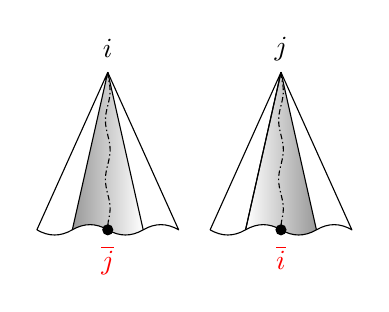
\begin{tikzpicture}[
edge from parent path=,
level distance=2cm,
level 1/.style={sibling distance=0.45cm}
%,scale=1, every node/.style={transform shape}
]

  \tikzstyle{ref}=[circle,fill=black,inner sep=0.5mm]
%  \tikzstyle{ref2}=[circle,fill=black!40,inner sep=0.5mm]
  \tikzstyle{dashdot}=[dashed,dash pattern=on 2pt off 1pt on 0.5pt off 1pt]
  \tikzstyle{mysnake}=[decorate,decoration={snake,amplitude=0.3mm,segment length=0.75cm}]

  \node (c1) {}
    child { node (c11) {} }
    child { node (c12) {} }
    child { node (c13) [ref,label={below:$\overline{j}$}] {} }
    child { node (c14) {} }
    child { node (c15) {} };

  \node (c10) [minimum height=0.5cm,node distance=0.3cm,above of=c1] {$i$};

  \draw [join=round] (c1.center)
    to (c11.center)
    to [bend right] (c12.center)
    -- cycle;

  \draw [join=round] (c12.center)
    to [bend left](c13.center) 
    to [bend right] (c14.center)
    to (c1.center);

  \draw [join=round] (c14.center)
    to [bend left] (c15.center)
    to (c1.center);

  \begin{pgfonlayer}{background}
  \path [right color=white,left color=black!40,shading=axis] (c12.center)
    to [bend left] (c13.center)
    to [bend right] (c14.center)
    to (c1.center);
  \draw [mysnake,dashdot] (c1.center) -- (c13.center);
  \end{pgfonlayer}


  \node (c2) [node distance=2.2cm,right of=c1] {}
    child { node (c22) {} }
    child { node (c23) {} }
    child { node (c24) [ref,label={below:$\overline{i}$}] {} }
    child { node (c25) {} }
    child { node (c26) {} };

  \node (c20) [minimum height=0.5cm,node distance=0.3cm,above of=c2] {$j$};

  \draw [join=round] (c2.center) -- (c23.center);

  \draw [join=round] (c2.center)
    to (c22.center) 
    to [bend right] (c23.center)
    -- cycle;

  \draw [join=round] (c23.center)
	to [bend left] (c24.center)
    to [bend right] (c25.center)
    to (c2.center);

  \draw [join=round] (c25.center)
    to [bend left] (c26.center) 
    to (c2.center);

  \begin{pgfonlayer}{background}
  \path [left color=white,right color=black!40,shading=axis] (c23.center)
    to [bend left] (c24.center)
    to [bend right] (c25.center)
    to (c2.center);
  \draw [mysnake,dashdot] (c2.center) -- (c24.center);
  \end{pgfonlayer}

\end{tikzpicture}
}}\\
    % \multicolumn{3}{c}{$\Updownarrow$}\\
    \multicolumn{3}{c}{$\Downarrow$}\\
    \parbox{0.33\textwidth}{\centering
%%%%%%%%%%%%%%%%%%%%%%%%%%%%%%%%%%%%%%%%%%%%%%%%%%%%%%%%%%%%%%%%%%%%%%%
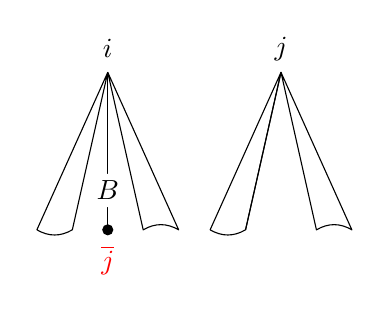
\begin{tikzpicture}[
edge from parent path=,
level distance=2cm,
level 1/.style={sibling distance=0.45cm}
%,scale=1, every node/.style={transform shape}
]

  \tikzstyle{ref}=[circle,fill=black,inner sep=0.5mm]
%  \tikzstyle{ref2}=[circle,fill=black!40,inner sep=0.5mm]
  \tikzstyle{dashdot}=[dashed,dash pattern=on 2pt off 1pt on 0.5pt off 1pt]
  \tikzstyle{mysnake}=[decorate,decoration={snake,amplitude=0.3mm,segment length=0.75cm}]

  \node (c1) {}
    child { node (c11) {} }
    child { node (c12) {} }
    child { node (c13) [ref,label={below:$\overline{j}$}] {} }
    child { node (c14) {} }
    child { node (c15) {} };

  \node (c10) [minimum height=0.5cm,node distance=0.3cm,above of=c1] {$i$};

  \draw [join=round] (c1.center)
    to (c11.center)
    to [bend right] (c12.center)
    -- cycle;

%  \draw [join=round] (c12.center)
%    to [bend right](c13.center) 
%    to [bend left] (c14.center)
%    to (c1.center);

  \draw (c1.center) to node [near end,circle,fill=white,inner sep=0.5pt] {$B$} (c13.center);

  \draw [join=round] (c1.center)
	to (c14.center)
    to [bend left] (c15.center)
    to (c1.center);

%  \begin{pgfonlayer}{background}
%  \path [left color=white,right color=black!40,shading=axis] (c12.center)
%    to [bend right] (c13.center)
%    to [bend left] (c14.center)
%    to (c1.center);
%  \draw [mysnake,dashdot] (c1.center) -- (c13.center);
%  \end{pgfonlayer}


  \node (c2) [node distance=2.2cm,right of=c1] {}
    child { node (c22) {} }
    child { node (c23) {} }
%    child { node (c24) [ref,label={below:$\overline{i}$}] {} }
    child { node (c24) {} }
    child { node (c25) {} }
    child { node (c26) {} };

  \node (c20) [minimum height=0.5cm,node distance=0.3cm,above of=c2] {$j$};

  \draw [join=round] (c2.center) -- (c23.center);

  \draw [join=round] (c2.center)
    to (c22.center) 
    to [bend right] (c23.center)
    -- cycle;

%  \draw [join=round] (c23.center)
%	to [bend left] (c24.center)
%    to [bend right] (c25.center)
%    to (c2.center);

  \draw [join=round] (c25.center)
    to [bend left] (c26.center) 
    to (c2.center) -- cycle;

%  \begin{pgfonlayer}{background}
%  \path [left color=white,right color=black!40,shading=axis] (c23.center)
%    to [bend left] (c24.center)
%    to [bend right] (c25.center)
%    to (c2.center);
%  \draw [mysnake,dashdot] (c2.center) -- (c24.center);
%  \end{pgfonlayer}

\end{tikzpicture}
} & + & \parbox{0.33\textwidth}{\centering
%%%%%%%%%%%%%%%%%%%%%%%%%%%%%%%%%%%%%%%%%%%%%%%%%%%%%%%%%%%%%%%%%%%%%%%
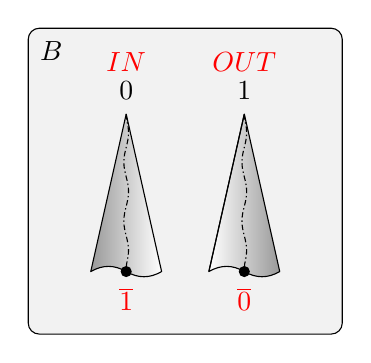
\begin{tikzpicture}[
edge from parent path=,
level distance=2cm,
level 1/.style={sibling distance=0.45cm}
%,scale=1, every node/.style={transform shape}
]

  \tikzstyle{ref}=[circle,fill=black,inner sep=0.5mm]
%  \tikzstyle{ref2}=[circle,fill=black!40,inner sep=0.5mm]
  \tikzstyle{dashdot}=[dashed,dash pattern=on 2pt off 1pt on 0.5pt off 1pt]
  \tikzstyle{mysnake}=[decorate,decoration={snake,amplitude=0.3mm,segment length=0.75cm}]

  \node (c1) {}
%    child { node (c11) {} }
    child { node (c12) {} }
    child { node (c13) [ref,label={below:$\overline{1}$}] {} }
    child { node (c14) {} };
%    child { node (c15) {} };

  \node (c10) [node distance=0.3cm,inner sep=0pt,above of=c1,label={above:$IN$}] {$0$};

%  \draw [join=round] (c1.center)
%    to (c11.center)
%    to [bend left] (c12.center)
%    -- cycle;

  \draw [join=round] (c12.center)
    to [bend left](c13.center) 
    to [bend right] (c14.center)
    to (c1.center) -- cycle;

%  \draw [join=round] (c14.center)
%    to [bend right] (c15.center)
%    to (c1.center);

  \node (c2) [node distance=1.5cm,right of=c1] {}
%    child { node (c22) {} }
    child { node (c23) {} }
    child { node (c24) [ref,label={below:$\overline{0}$}] {} }
    child { node (c25) {} };
%    child { node (c26) {} };

  \node (c20) [node distance=0.3cm,inner sep=0pt,above of=c2,label={above:$OUT$}] {$1$};

  \draw [join=round] (c2.center) -- (c23.center);

%  \draw [join=round] (c2.center)
%    to (c22.center) 
%    to [bend right] (c23.center)
%    -- cycle;

  \draw [join=round] (c23.center)
	to [bend left] (c24.center)
    to [bend right] (c25.center)
    to (c2.center) -- cycle;

%  \draw [join=round] (c25.center)
%    to [bend left] (c26.center) 
%    to (c2.center);

  \node [yshift=0.8cm,node distance=0.95cm,left of=c1] {$B$};

  \begin{pgfonlayer}{background}
  \node [rounded corners=4pt,draw,fill=black!5,fit=(c1) (c10) (c12) (c14) (c2) (c20) (c23) (c25),inner sep=0.67cm] {};

  \path [right color=white,left color=black!40,shading=axis] (c12.center)
    to [bend left] (c13.center)
    to [bend right] (c14.center)
    to (c1.center);
  \draw [mysnake,dashdot] (c1.center) -- (c13.center);

  \path [left color=white,right color=black!40,shading=axis] (c23.center)
    to [bend left] (c24.center)
    to [bend right] (c25.center)
    to (c2.center);
  \draw [mysnake,dashdot] (c2.center) -- (c24.center);
  \end{pgfonlayer}

\end{tikzpicture}
}
  \end{tabular}

  \caption{An illustration of elimination of Type~3 cut-points. First, the two components are
  sliced at their accepting states. Next, the kernels of the result containing
  references to~$i$ and~$j$ are transformed into a~new box~$B$, which is added to the remaining part of the component~$i$.
  Finally, the modified component~$j$ contains no references to~$i$.}
  \label{fig:type3folding}
\end{figure}

%--------------------------------------------
\subsubsection*{Type~3 Cut-point Elimination}
% \paragraph{Type~3.}
To eliminate a pair of Type~3 cut-points $i$ and $j$ (i.e., the cut-points
mutually referencing
each other---see Fig.~\ref{fig:t3cutpoint}), we need to use a~box encoding a~cycle
starting at cut-point $i$ going through cut-point $j$ and, finally, back to~$i$ (this
corresponds, e.g., to a pair of forward and backward links in a doubly-linked list).
Intuitively, we create a box composed of two components (unlike cut-points of
Type~1 and~2,
which have only a single component). The first component of the box will be made from the part of the
$i$-th component that contains all references to $j$. Similarly, the second component of
the box will be made from the part of the $j$-th that contains all references to $i$. 
As a result, the box will represent a sub-graph containing the loop between the roots of the original $i$-th and $j$-th component.

Let us describe the elimination of Type~3 cut-point in a greater detail. First, we perform
slicing of components~$i$ and~$j$, which mutually refer each other, such that
the kernels obtained in the slicing
contain all paths from~$i$ to~$j$ (resp.\ from~$j$ to~$i$).
The two kernels are
transformed into a box~$B$. The box~$B$ is then appended to the accepting transitions of
the residue of the component~$i$ in the same way as in the previous cases. As the last step,
we replace (i)~the component~$i$ within the original FA by the modified residue
and (ii)~the component~$j$ by the residue of component~$j$.
As a~result, the new component~$i$ contains a~single reference to~$j$, and the
new component~$j$ contains no reference to~$i$---see
Fig.~\ref{fig:type3folding}.

Note that we could also perform the symmetrical transformation in which the newly created
box is added into the component~$j$. This would yield a~different structure with the same
semantics. In order to decide which variant to choose in practice, we use an ordering on
the set of components of the original FA, i.e., if $i < j$, we append the newly created
box to the residue of~$i$.

%*******************************************************************************
\subsection{From Nested FAs to Alphabet Symbols}
%*******************************************************************************

When performing certain automata operations,
such as language inclusion, we treat all symbols as not having any underlying
structure at all.
To make this work, we have to ensure that the nested FAs (boxes) with the same
semantics are represented using the same alphabet symbol.
This is achieved by maintaining
a~database that maps boxes to alphabet symbols. Every time a~new box is created, it is
first compared to existing boxes having the same root interconnection graph (cf.\ \secref{sec:icgraph}) (which also
implies the same number of components).
The comparison of two boxes is done via checking
language equality of their underlying FAs\footnote{
Here, we are not dealing with sets of FAs, hence the comparison of two FAs can
be done component-wise.
}\footnote{The language equality check is performed as two inclusion queries.
The inclusion test itself is again only a~safe approximation, since we ignore the structure
of nested boxes that can appear within the box we have just created. Therefore,
it can be the case that two boxes with the same semantics are represented by different
alphabet symbols. According to our experiments, such approximation, however,
works well in practice.
}.
If the same box already exists, the symbol obtained from the database is used for its
representation. Otherwise, a~new alphabet symbol is created and
stored in the database.

Furthermore, we can also consider only language inclusion to relax the requirement of
equality when testing whether the two boxes match. This means that during the folding the
given box can be potentially replaced by a~``bigger'' one that already exists in the
database. As discussed later, this can in some cases drastically decrease the number of
boxes that are required, and thus substantially increase the performance.

%\ol{say that the discovered boxes are folded according to \secref{sec:box_folding}}

% \ol{copied from previous, obsolete; we need to give a proper folding section}
% \comment[lh]{don't know what you mean but I thought that the folding unfolding below should be usable as an interface between refinement paper and thesis of jiri, it should be possible to present the part from Jiri thesis as a concretization of details in the paragraphs below.}
%
% \renewcommand{\boxtas}{{\ta_\iport \ta_2 \cdots \ta_{n} {\kword{\ta_{\oport_##1}}}}}   % box components
% \renewcommand{\boxtasin}[0]{\ta_\iport^\botox \ta_2 \cdots \ta_{n} {\kword{\ta_{\oport_##1}^\botox}}}   % box components
% The folding operation assumes that the concerned FA is first transformed into the form
% $\fa = \tuple{\boxtas \ta_1' \cdots \ta_m',\asgn}$ by a sequence of splitting,
% cutting, and swapping.
% %
% The tuple of TAs $\boxtas$ will then be folded into a new box $\botox$
% with~$\ta_\iport$ as its input component and~$\kseq{\ta_{\oport_{#1}}}$ as its output components.
% Moreover, the operation is given sets of selectors~$S_{\iport},
% \kseq{S_{\oport_{#1}}}$ of roots of components in~$\ta_\iport$ and~$\kseq{\ta_{\oport_{#1}}}$, respectivelly, that are to
% be folded into~$\botox$.
% %
% The box~$\botox =
% \tuple{\boxtasin,\{\iport\mapsto 1,\kseq{\oport_{#1}\mapsto n+{#1}}\}}$
%  arises from~$\fa$ by taking $\boxtas$
% %
% and by removing selectors that are not in $S_{\iport}$ and $\kseq{S_{\oport_{#1}}}$
% from root rules of $\ta_\iport$ and~$\kseq{\ta_{\oport_{#1}}}$ to obtain $\ta_\iport^\botox$ and
% $\kseq{\ta_{\oport_{#1}}^\botox}$, respectively.
%
% Folding returns the forest automaton $\fa' = \tuple{\ta'_{\iport}
% \kword{\ta'_{\oport_{#1}}} \ta'_1 \cdots \ta'_m, \asgn'}$ that arises from $\fa$ as follows.
% All successors of the roots accepted in $\ta_\iport$ and $\kseq{\ta_{\oport_{#1}}}$
% reachable over selectors from $S_\iport$ and $\kseq{S_{\oport_#1}}$
% are removed in $\ta'_\iport$ and $\kseq{\ta'_{\oport_{#1}}}$ respectively (since they are enclosed in~$\botox$).
% The root of the trees of $\ta'_\iport$ gets an additional edge labelled by
% $\botox$, leading to the reference $\rr n$ (the output port),
% and the components $\ta_2 \cdots \ta_{n}$ are removed (since they are also enclosed in~$\botox$).
% %
% This operation is denoted as $\folding{n,S_{\iport},\kseq{S_{\oport_{#1}}},\botox}$.

% %------------------------------------------------------------------------------
% \old{
% \paragraph{Folding of boxes.}
% The folding operation assumes that the concerned FA is first transformed into the form
% $\fa = \tuple{\boxtas \ta_1' \cdots \ta_m',\asgn}$ by a sequence of splitting,
% cutting, and swapping.
% %
% % where all trees of $\langof{\ta_\iport}$ and $\langof{\ta_\oport}$ are of depth~$1$. 
% %
% The tuple of TAs $\boxtas$ will then be folded into a new box $\botox$
% with~$\ta_\iport$ as its input component and~$\ta_\oport$ as its output.
% Moreover, the operation is given sets of selectors~$S_{\iport},
% S_{\oport}$ of roots of components in~$\ta_\iport$ and~$\ta_\oport$ that are to
% be folded into~$\botox$.
% %
% The box~$\botox =
% \tuple{\boxtasin,\{\iport\mapsto 1,\oport\mapsto n\}}$
%  arises from~$\fa$ by taking $\boxtas$
% %
% and by removing selectors that are not in $S_{\iport}$ and $S_{\oport}$
% from root rules of $\ta_\iport$ and~$\ta_\oport$ to obtain $\ta_\iport^\botox$ and
% $\ta_\oport^\botox$ respectively.
% %, which results into $\ta_1'$ and $\ta_n$'. 
% % Particularly, the roots of $\ta_\iport$ and $\ta_\oport$ are stripped from all
% % successors but those 
% % reached by selectors from sets $S_\iport$ and $S_\oport$ of selectors, respectively. 
% %
% %Intuitively, the box $\botox$ will enclose only selectors leading from its
% %input and output ports that are from the two sets, the rest will be left outside
% %the box.
% %
%
% Folding returns the forest automaton $\fa' = \tuple{\ta'_{\iport}
% \ta'_{\oport} \ta'_1 \cdots \ta'_m, \asgn'}$ that arises from $\fa$ as follows.
% All successors of the roots accepted in $\ta_\iport$ and $\ta_\oport$
% reachable over selectors from $S_\iport$ and $S_\oport$
% are removed in $\ta'_\iport$ and $\ta'_\oport$ respectively (since they are enclosed in~$\botox$).
% The root of the trees of $\ta'_\iport$ gets an additional edge labelled by
% $\botox$, leading to the reference $\rr n$ (the output port),
% and the components $\ta_2 \cdots \ta_{n-1}$ are removed (since they are also enclosed in~$\botox$).
% %
% This operation is denoted as $\folding{n,S_{\iport},S_{\oport},\botox}$.
% %
% % $\fa' = \folding{n,S_{\iport},S_{\oport},\botox}(\fa)$ such that 
% %$\semof{\fa'} = \semof{\fa}$
% %For every $\heap'\in\langof{\fa'}$, 
% %there is $\heap\in\langof\fa$ 
% %such that $\heap'\unfoldof{(u,\botox,v)}{blah}\heap$,
% %$u$ is the $i$-th root in the forest decomposition of $\heap$ accepted by $\fa$
% %and also the $j$-th root in the forest decomposition of $\heap'$ accepted by $\fa'$.
% %Algorithms for learning boxes and folding are described in \cite{}.
% %%%
%
% %------------------------------------------------------------------------------
% \paragraph{Unfolding of boxes.} 
% Unfolding is called as a preprocessing step before operations that implement
% program statements
% in order to expose the selectors accessed by the statement. 
% It is called after a sequence of cutting, splitting, and swapping
% that changes the forest automaton into the form 
% $\fa' = \tuple{\ta_\iport'\ta_\oport'\ta_1'\cdots\ta_m',\asgn'}$ where
% %
% % all trees of $\langof{\ta_\iport'}$ and $\langof{\ta_\oport'}$, are of
% % depth~$1$, and
% %
% trees of $\ta'_\iport$ have a~reference $\overline 2$ to $\ta_\oport'$ accessible by an 
% edge going from the root and labelled by the box~$\botox$ that is to be unfolded.
% %
% Furthermore, assume that the box $\botox$ is of the form
% $\tuple{\boxtasin,\{\iport\mapsto 1,\oport\mapsto n\}}$
% %
% and 
% %
% the input and the output ports have outgoing selectors from the sets 
% $S_\iport$ and $S_\oport$ respectively. 
% %
% The operation returns the forest automaton 
% $\fa$ that arises from~$\fa'$ by 
% %$\tuple{\ta_\iport'',\tas,\ta_\oport'',\{\iport\mapsto 1,\oport\mapsto n+1\}}$
% %
% inserting components $\boxtasin$ in between $\ta'_\iport$ and $\ta'_\oport$, 
% removing the $\botox$ successor of the root in~$\ta_\iport'$,
% merging $\ta_\iport^\botox$ with $\ta_\iport'$, and $\ta_\oport^\botox$
% with $\ta_\oport'$.
% % The merging on the language level consists of merging roots of the trees.
% The merging on the TA level consists of merging root transitions of the TAs.
% %
% We denote this operation as $\unfolding{n,S_{\iport},\kseq{S_{\oport_{#1}}},\botox}$.
% }

%\comment[ar]{We may add a figure of folding and unfolding}

%*******************************************************************************
\section{Running Example}
\label{sec:running_example}
%*******************************************************************************


\usetikzlibrary{calc,matrix,backgrounds,fit,shapes,arrows}
\newcommand{\circulardll}[1]{
\begin{tikzpicture}[
  scale=1.0,
  transform shape,
  node distance=18mm,
%  >=stealth',
  >=latex,
  grow=up,
  edge from parent/.style={draw,->},
  edge from parent path={(\tikzparentnode.north) -- (\tikzchildnode.south)},
  level distance=8mm,
  level 1/.style={sibling distance=10mm},
  level 2/.style={sibling distance=6mm},
]

  \path[use as bounding box] (-38mm,-38mm) rectangle (38mm,38mm);

  \tikzstyle{memnode}=[draw,rectangle,fill=lightgray,thick,minimum height=4.5mm, minimum width=4.5mm,inner sep=1mm,node distance=18mm,font=\tt]
  \tikzstyle{smallmemnode}=[draw,rectangle,fill=lightgray,thick,minimum height=2.5mm, minimum width=2.5mm,inner sep=1mm,node distance=18mm,font=\tt]
  \tikzstyle{memnodeblue}=[draw,rectangle,fill=blue!30,thick,minimum height=4.5mm, minimum width=4.5mm,inner sep=1mm,node distance=18mm,font=\tt]
  \tikzstyle{memnodepink}=[draw,rectangle,fill=red!30,thick,minimum height=4.5mm, minimum width=4.5mm,inner sep=1mm,node distance=18mm,font=\tt]
  \tikzstyle{memnodegreen}=[draw,rectangle,fill=green!60,thick,minimum height=4.5mm, minimum width=4.5mm,inner sep=1mm,node distance=18mm,font=\tt]
  \tikzstyle{memnodepurple}=[draw,rectangle,fill=purple!60,thick,minimum height=4.5mm, minimum width=4.5mm,inner sep=1mm,node distance=18mm,font=\tt]
  \tikzstyle{memnodeorange}=[draw,rectangle,fill=orange!60,thick,minimum height=4.5mm, minimum width=4.5mm,inner sep=1mm,node distance=18mm,font=\tt]

  % number of nodes on the circular list
  \def \n {#1}


  \tikzstyle{nullnode}=[node distance=18mm,label=center:$\bot$]
  \tikzstyle{varnode}=[font=\tt]
  \tikzstyle{refnode}=[fill=lightgray!40,minimum height=4.5mm, minimum width=4.5mm,inner sep=1mm,font=\tt]

  \tikzstyle{pointer}=[draw,->,>=latex]

  \foreach \x in {1, ..., \n}
  {
    \begin{scope}
    [
      rotate=360/\n*\x
    ]
    \node[memnode] (q \x) at (0mm,14mm) {}
     child {node[smallmemnode] {}
       child {node[smallmemnode] {}}
       child {node[smallmemnode] {}} 
     }
     child {node[smallmemnode] {}
       child {node[smallmemnode] {}}
       child {node[smallmemnode] {}} 
    };

    \draw[pointer,bend left] (q \x-1) edge (q \x);
    \draw[pointer,bend left=45] (q \x-1-1) edge (q \x);
    \draw[pointer] (q \x-1-2) edge (q \x);

    \draw[pointer,bend right] (q \x-2) edge (q \x);
    \draw[pointer,bend right=45] (q \x-2-2) edge (q \x);
    \draw[pointer] (q \x-2-1) edge (q \x);

	\pgfmathparse{int(mod(\x,4))}
    \ifnum\pgfmathresult=0
		\node[smallmemnode,fill=green,above right of=q \x-1-2,node distance=8mm,xshift=-3mm] (q \x add) {};
        \draw[pointer] (q \x-1-1) -- (q \x add);
        \draw[pointer,bend right=15] (q \x add) edge (q \x);
    \fi
    \ifnum\pgfmathresult=1
		\node[smallmemnode,fill=red!30,above right of=q \x-1-1,node distance=8mm,xshift=-3mm] (q \x add) {};
        \draw[pointer] (q \x-1-1) -- (q \x add);
        \draw[pointer,bend right=15] (q \x add) edge (q \x);
    \fi
    \ifnum\pgfmathresult=2
		\node[smallmemnode,fill=blue!40,above right of=q \x-2-1,node distance=8mm,xshift=-3mm] (q \x add) {};
        \draw[pointer] (q \x-2-1) -- (q \x add);
        \draw[pointer,bend right=5] (q \x add) edge (q \x);
    \fi
    \ifnum\pgfmathresult=3
		\node[smallmemnode,fill=purple!70,above left of=q \x-2-1,node distance=8mm,xshift=3mm] (q \x add1) {};
        \draw[pointer] (q \x-2-1) -- (q \x add1);
		\node[smallmemnode,fill=brown!80,above right of=q \x-1-2,node distance=8mm,xshift=-3mm] (q \x add2) {};
        \draw[pointer] (q \x-1-2) -- (q \x add2);
        \draw[pointer,bend right=5] (q \x add1) edge (q \x);
        \draw[pointer,bend left=5] (q \x add2) edge (q \x);
    \fi




    %\node[smallmemnode] at (0mm,30mm) {};
    %\draw (q \x) -- +(0mm,10mm);
    \end{scope}
  }

  \foreach \x [evaluate=\x as \xprev using int(\x-1)] in {1, ..., \n}
  {
    \ifnum\x>1
      \draw[pointer,bend left] (q \x) edge (q \xprev);
      \draw[pointer,bend left] (q \xprev) edge (q \x);
    \else
      \draw[pointer,bend left] (q \x) edge (q \n);
      \draw[pointer,bend left] (q \n) edge (q \x);
    \fi
  }

\end{tikzpicture}}

%\circulardll{5}

% include the \circulardlltreefold{n} command
\usetikzlibrary{calc,matrix,backgrounds,fit,shapes,arrows}
\newcommand{\circulardlltreefold}[1]{
\begin{tikzpicture}[
  scale=1.0,
  transform shape,
  node distance=18mm,
%  >=stealth',
  >=latex,
  grow=up,
  edge from parent/.style={draw,->},
  edge from parent path={(\tikzparentnode.north) -- (\tikzchildnode.south)},
  level distance=8mm,
  level 1/.style={sibling distance=10mm},
  level 2/.style={sibling distance=6mm},
]

  \path[use as bounding box] (-38mm,-38mm) rectangle (38mm,38mm);

  \tikzstyle{memnode}=[draw,rectangle,fill=lightgray,thick,minimum height=4.5mm, minimum width=4.5mm,inner sep=1mm,node distance=18mm,font=\tt]
  \tikzstyle{smallmemnode}=[draw,rectangle,fill=lightgray,thick,minimum height=2.5mm, minimum width=2.5mm,inner sep=1mm,node distance=18mm,font=\tt]
  \tikzstyle{memnodeblue}=[draw,rectangle,fill=blue!30,thick,minimum height=4.5mm, minimum width=4.5mm,inner sep=1mm,node distance=18mm,font=\tt]
  \tikzstyle{memnodepink}=[draw,rectangle,fill=red!30,thick,minimum height=4.5mm, minimum width=4.5mm,inner sep=1mm,node distance=18mm,font=\tt]
  \tikzstyle{memnodegreen}=[draw,rectangle,fill=green!60,thick,minimum height=4.5mm, minimum width=4.5mm,inner sep=1mm,node distance=18mm,font=\tt]
  \tikzstyle{memnodepurple}=[draw,rectangle,fill=purple!60,thick,minimum height=4.5mm, minimum width=4.5mm,inner sep=1mm,node distance=18mm,font=\tt]
  \tikzstyle{memnodeorange}=[draw,rectangle,fill=orange!60,thick,minimum height=4.5mm, minimum width=4.5mm,inner sep=1mm,node distance=18mm,font=\tt]

  % number of nodes on the circular list
  \def \n {#1}


  \tikzstyle{nullnode}=[node distance=18mm,label=center:$\bot$]
  \tikzstyle{varnode}=[font=\tt]
  \tikzstyle{refnode}=[fill=lightgray!40,minimum height=4.5mm, minimum width=4.5mm,inner sep=1mm,font=\tt]

  \tikzstyle{pointer}=[draw,->,>=latex]

  \foreach \x in {1, ..., \n}
  {
    \begin{scope}
    [
      rotate=360/\n*\x
    ]

    \fill[red!30] plot[dashed,fill=black,smooth cycle] coordinates{(0mm,9mm) (10mm,28mm) (-10mm,28mm)};

    \node[memnode] (q \x) at (0mm,14mm) {}
     child {node[smallmemnode] {}
       child {node {} edge from parent[dotted]}
       child {node {} edge from parent[dotted]} 
     }
     child {node[smallmemnode] {}
       child {node {} edge from parent[dotted]}
       child {node {} edge from parent[dotted]} 
    };

    \draw[pointer,bend left] (q \x-1) edge (q \x);
    \draw[pointer,dotted,bend left=45] (q \x-1-1) edge (q \x);
    \draw[pointer,dotted] (q \x-1-2) edge (q \x);

    \draw[pointer,bend right] (q \x-2) edge (q \x);
    \draw[pointer,dotted,bend right=45] (q \x-2-2) edge (q \x);
    \draw[pointer,dotted] (q \x-2-1) edge (q \x);

%	\pgfmathparse{int(mod(\x,4))}
%    \ifnum\pgfmathresult=0
%		\node[smallmemnode,above right of=q \x-1-2,node distance=8mm,xshift=-3mm] (q \x add) {};
%        \draw[pointer] (q \x-1-1) -- (q \x add);
%        \draw[pointer,bend right=15] (q \x add) edge (q \x);
%    \fi
%    \ifnum\pgfmathresult=1
%		\node[smallmemnode,above right of=q \x-1-1,node distance=8mm,xshift=-3mm] (q \x add) {};
%        \draw[pointer] (q \x-1-1) -- (q \x add);
%        \draw[pointer,bend right=15] (q \x add) edge (q \x);
%    \fi
%    \ifnum\pgfmathresult=2
%		\node[smallmemnode,above right of=q \x-2-1,node distance=8mm,xshift=-3mm] (q \x add) {};
%        \draw[pointer] (q \x-2-1) -- (q \x add);
%        \draw[pointer,bend right=5] (q \x add) edge (q \x);
%    \fi
%    \ifnum\pgfmathresult=3
%		\node[smallmemnode,above left of=q \x-2-1,node distance=8mm,xshift=3mm] (q \x add1) {};
%        \draw[pointer] (q \x-2-1) -- (q \x add1);
%		\node[smallmemnode,above right of=q \x-1-2,node distance=8mm,xshift=-3mm] (q \x add2) {};
%        \draw[pointer] (q \x-1-2) -- (q \x add2);
%        \draw[pointer,bend right=5] (q \x add1) edge (q \x);
%        \draw[pointer,bend left=5] (q \x add2) edge (q \x);
%    \fi




    %\node[smallmemnode] at (0mm,30mm) {};
    %\draw (q \x) -- +(0mm,10mm);
    \end{scope}
  }

  \foreach \x [evaluate=\x as \xprev using int(\x-1)] in {1, ..., \n}
  {
    \ifnum\x>1
      \draw[pointer,bend left] (q \x) edge (q \xprev);
      \draw[pointer,bend left] (q \xprev) edge (q \x);
    \else
      \draw[pointer,bend left] (q \x) edge (q \n);
      \draw[pointer,bend left] (q \n) edge (q \x);
    \fi
  }

\end{tikzpicture}}

%\circulardlltreefold{5}

% include the \circulardlltreefolded{n} command
\usetikzlibrary{calc,matrix,backgrounds,fit,shapes,arrows}
\newcommand{\circulardlltreefolded}[1]{
\begin{tikzpicture}[
  scale=1.0,
  transform shape,
  node distance=18mm,
%  >=stealth',
  >=latex,
  grow=up,
  edge from parent/.style={draw,->},
  edge from parent path={(\tikzparentnode.north) -- (\tikzchildnode.south)},
  level distance=18mm,
  level 1/.style={sibling distance=10mm},
  level 2/.style={sibling distance=6mm},
]

  \path[use as bounding box] (-38mm,-38mm) rectangle (38mm,38mm);

  \tikzstyle{memnode}=[draw,rectangle,fill=lightgray,thick,minimum height=4.5mm, minimum width=4.5mm,inner sep=1mm,node distance=18mm,font=\tt]
  \tikzstyle{smallmemnode}=[draw,rectangle,fill=lightgray,thick,minimum height=2.5mm, minimum width=2.5mm,inner sep=1mm,node distance=18mm,font=\tt]
  \tikzstyle{memnodeblue}=[draw,rectangle,fill=blue!30,thick,minimum height=4.5mm, minimum width=4.5mm,inner sep=1mm,node distance=18mm,font=\tt]
  \tikzstyle{memnodepink}=[draw,rectangle,fill=red!30,thick,minimum height=4.5mm, minimum width=4.5mm,inner sep=1mm,node distance=18mm,font=\tt]
  \tikzstyle{memnodegreen}=[draw,rectangle,fill=green!60,thick,minimum height=4.5mm, minimum width=4.5mm,inner sep=1mm,node distance=18mm,font=\tt]
  \tikzstyle{memnodepurple}=[draw,rectangle,fill=purple!60,thick,minimum height=4.5mm, minimum width=4.5mm,inner sep=1mm,node distance=18mm,font=\tt]
  \tikzstyle{memnodeorange}=[draw,rectangle,fill=orange!60,thick,minimum height=4.5mm, minimum width=4.5mm,inner sep=1mm,node distance=18mm,font=\tt]

  % number of nodes on the circular list
  \def \n {#1}


  \tikzstyle{nullnode}=[node distance=18mm,label=center:$\bot$]
  \tikzstyle{varnode}=[font=\tt]
  \tikzstyle{refnode}=[fill=lightgray!40,minimum height=4.5mm, minimum width=4.5mm,inner sep=1mm,font=\tt]

  \tikzstyle{pointer}=[draw,->,>=latex]

  \foreach \x in {1, ..., \n}
  {
    \begin{scope}
    [
      rotate=360/\n*\x
    ]

%    \fill[red!30] plot[dashed,fill=black,smooth cycle] coordinates{(0mm,9mm) (10mm,28mm) (-10mm,28mm)};

    \node[memnode] (q \x) at (0mm,14mm) {}
     child {node {}
%       child {node {} edge from parent[dotted]}
%       child {node {} edge from parent[dotted]} 
%     }
%     child {node[smallmemnode] {}
%       child {node {} edge from parent[dotted]}
%       child {node {} edge from parent[dotted]} 
    };

    \node[fill=red!30,draw,inner sep=1mm,rotate=90,anchor=west] at(-4mm,18mm) {tree-rootptr};

%    \draw[pointer,bend left] (q \x-1) edge (q \x);
%    \draw[pointer,bend left=45] (q \x-1-1) edge (q \x);
%    \draw[pointer] (q \x-1-2) edge (q \x);

%    \draw[pointer,bend right] (q \x-2) edge (q \x);
%    \draw[pointer,bend right=45] (q \x-2-2) edge (q \x);
%    \draw[pointer] (q \x-2-1) edge (q \x);

%	\pgfmathparse{int(mod(\x,4))}
%    \ifnum\pgfmathresult=0
%		\node[smallmemnode,above right of=q \x-1-2,node distance=8mm,xshift=-3mm] (q \x add) {};
%        \draw[pointer] (q \x-1-1) -- (q \x add);
%        \draw[pointer,bend right=15] (q \x add) edge (q \x);
%    \fi
%    \ifnum\pgfmathresult=1
%		\node[smallmemnode,above right of=q \x-1-1,node distance=8mm,xshift=-3mm] (q \x add) {};
%        \draw[pointer] (q \x-1-1) -- (q \x add);
%        \draw[pointer,bend right=15] (q \x add) edge (q \x);
%    \fi
%    \ifnum\pgfmathresult=2
%		\node[smallmemnode,above right of=q \x-2-1,node distance=8mm,xshift=-3mm] (q \x add) {};
%        \draw[pointer] (q \x-2-1) -- (q \x add);
%        \draw[pointer,bend right=5] (q \x add) edge (q \x);
%    \fi
%    \ifnum\pgfmathresult=3
%		\node[smallmemnode,above left of=q \x-2-1,node distance=8mm,xshift=3mm] (q \x add1) {};
%        \draw[pointer] (q \x-2-1) -- (q \x add1);
%		\node[smallmemnode,above right of=q \x-1-2,node distance=8mm,xshift=-3mm] (q \x add2) {};
%        \draw[pointer] (q \x-1-2) -- (q \x add2);
%        \draw[pointer,bend right=5] (q \x add1) edge (q \x);
%        \draw[pointer,bend left=5] (q \x add2) edge (q \x);
%    \fi




    %\node[smallmemnode] at (0mm,30mm) {};
    %\draw (q \x) -- +(0mm,10mm);
    \end{scope}
  }

  \foreach \x [evaluate=\x as \xprev using int(\x-1)] in {1, ..., \n}
  {
    \ifnum\x>1
      \draw[pointer,bend left] (q \x) edge (q \xprev);
      \draw[pointer,bend left] (q \xprev) edge (q \x);
    \else
      \draw[pointer,bend left] (q \x) edge (q \n);
      \draw[pointer,bend left] (q \n) edge (q \x);
    \fi
  }

\end{tikzpicture}}

%\circulardlltreefolded{5}

% include the \circulardlldllfold{n} command
\usetikzlibrary{calc,matrix,backgrounds,fit,shapes,arrows}
\newcommand{\circulardlldllfold}[1]{
\begin{tikzpicture}[
  scale=1.0,
  transform shape,
  node distance=18mm,
%  >=stealth',
  >=latex,
  grow=up,
  edge from parent/.style={draw,->},
  edge from parent path={(\tikzparentnode.north) -- (\tikzchildnode.south)},
  level distance=18mm,
  level 1/.style={sibling distance=10mm},
  level 2/.style={sibling distance=6mm},
]

  \path[use as bounding box] (-38mm,-38mm) rectangle (38mm,38mm);

  \tikzstyle{memnode}=[draw,rectangle,fill=lightgray,thick,minimum height=4.5mm, minimum width=4.5mm,inner sep=1mm,node distance=18mm,font=\tt]
  \tikzstyle{smallmemnode}=[draw,rectangle,fill=lightgray,thick,minimum height=2.5mm, minimum width=2.5mm,inner sep=1mm,node distance=18mm,font=\tt]
  \tikzstyle{memnodeblue}=[draw,rectangle,fill=blue!30,thick,minimum height=4.5mm, minimum width=4.5mm,inner sep=1mm,node distance=18mm,font=\tt]
  \tikzstyle{memnodepink}=[draw,rectangle,fill=red!30,thick,minimum height=4.5mm, minimum width=4.5mm,inner sep=1mm,node distance=18mm,font=\tt]
  \tikzstyle{memnodegreen}=[draw,rectangle,fill=green!60,thick,minimum height=4.5mm, minimum width=4.5mm,inner sep=1mm,node distance=18mm,font=\tt]
  \tikzstyle{memnodepurple}=[draw,rectangle,fill=purple!60,thick,minimum height=4.5mm, minimum width=4.5mm,inner sep=1mm,node distance=18mm,font=\tt]
  \tikzstyle{memnodeorange}=[draw,rectangle,fill=orange!60,thick,minimum height=4.5mm, minimum width=4.5mm,inner sep=1mm,node distance=18mm,font=\tt]

  % number of nodes on the circular list
  \def \n {#1}


  \tikzstyle{nullnode}=[node distance=18mm,label=center:$\bot$]
  \tikzstyle{varnode}=[font=\tt]
  \tikzstyle{refnode}=[fill=lightgray!40,minimum height=4.5mm, minimum width=4.5mm,inner sep=1mm,font=\tt]

  \tikzstyle{pointer}=[draw,->,>=latex]

  \foreach \x in {1, ..., \n}
  {
    \begin{scope}
    [
      rotate=360/\n*\x
    ]

%    \fill[red!30] plot[dashed,fill=black,smooth cycle] coordinates{(0mm,9mm) (10mm,28mm) (-10mm,28mm)};

    \node[memnode] (q \x) at (0mm,14mm) {}
     child {node {}
%       child {node {} edge from parent[dotted]}
%       child {node {} edge from parent[dotted]} 
%     }
%     child {node[smallmemnode] {}
%       child {node {} edge from parent[dotted]}
%       child {node {} edge from parent[dotted]} 
    };

    \node[fill=red!30,draw,inner sep=1mm,rotate=90,anchor=west] at(-4mm,18mm) {tree-rootptr};

%    \draw[pointer,bend left] (q \x-1) edge (q \x);
%    \draw[pointer,bend left=45] (q \x-1-1) edge (q \x);
%    \draw[pointer] (q \x-1-2) edge (q \x);

%    \draw[pointer,bend right] (q \x-2) edge (q \x);
%    \draw[pointer,bend right=45] (q \x-2-2) edge (q \x);
%    \draw[pointer] (q \x-2-1) edge (q \x);

%	\pgfmathparse{int(mod(\x,4))}
%    \ifnum\pgfmathresult=0
%		\node[smallmemnode,above right of=q \x-1-2,node distance=8mm,xshift=-3mm] (q \x add) {};
%        \draw[pointer] (q \x-1-1) -- (q \x add);
%        \draw[pointer,bend right=15] (q \x add) edge (q \x);
%    \fi
%    \ifnum\pgfmathresult=1
%		\node[smallmemnode,above right of=q \x-1-1,node distance=8mm,xshift=-3mm] (q \x add) {};
%        \draw[pointer] (q \x-1-1) -- (q \x add);
%        \draw[pointer,bend right=15] (q \x add) edge (q \x);
%    \fi
%    \ifnum\pgfmathresult=2
%		\node[smallmemnode,above right of=q \x-2-1,node distance=8mm,xshift=-3mm] (q \x add) {};
%        \draw[pointer] (q \x-2-1) -- (q \x add);
%        \draw[pointer,bend right=5] (q \x add) edge (q \x);
%    \fi
%    \ifnum\pgfmathresult=3
%		\node[smallmemnode,above left of=q \x-2-1,node distance=8mm,xshift=3mm] (q \x add1) {};
%        \draw[pointer] (q \x-2-1) -- (q \x add1);
%		\node[smallmemnode,above right of=q \x-1-2,node distance=8mm,xshift=-3mm] (q \x add2) {};
%        \draw[pointer] (q \x-1-2) -- (q \x add2);
%        \draw[pointer,bend right=5] (q \x add1) edge (q \x);
%        \draw[pointer,bend left=5] (q \x add2) edge (q \x);
%    \fi




    %\node[smallmemnode] at (0mm,30mm) {};
    %\draw (q \x) -- +(0mm,10mm);
    \end{scope}
  }

  \foreach \x [evaluate=\x as \xprev using int(\x-1)] in {1, ..., \n}
  {
    \ifnum\x>1
      \begin{pgfonlayer}{background}
        \node[fill=blue!60,opacity=0.5,rounded corners,rotate fit=(360/\n*(\x))-(180/\n),fit=(q \xprev) (q \x)] {};
      \end{pgfonlayer}
      \draw[pointer,bend left] (q \x) edge (q \xprev);
      \draw[pointer,bend left] (q \xprev) edge (q \x);
    \else
      \begin{pgfonlayer}{background}
        \node[fill=blue!60,opacity=0.5,rounded corners,rotate fit=(360/\n*(\x))-(180/\n),fit=(q \x) (q \n)] {};
      \end{pgfonlayer}
      \draw[pointer,bend left] (q \x) edge (q \n);
      \draw[pointer,bend left] (q \n) edge (q \x);
    \fi
  }

\end{tikzpicture}}

%\circulardlldllfold{5}
% include the \circulardlldllfolded{n} command
\usetikzlibrary{calc,matrix,backgrounds,fit,shapes,arrows}
\newcommand{\circulardlldllfolded}[1]{
\begin{tikzpicture}[
  scale=1.0,
  transform shape,
  node distance=18mm,
%  >=stealth',
  >=latex,
  grow=up,
  edge from parent/.style={draw,->},
  edge from parent path={(\tikzparentnode.north) -- (\tikzchildnode.south)},
  level distance=18mm,
  level 1/.style={sibling distance=10mm},
  level 2/.style={sibling distance=6mm},
]

  \path[use as bounding box] (-38mm,-38mm) rectangle (38mm,38mm);

  \tikzstyle{memnode}=[draw,rectangle,fill=lightgray,thick,minimum height=4.5mm, minimum width=4.5mm,inner sep=1mm,node distance=18mm,font=\tt]
  \tikzstyle{smallmemnode}=[draw,rectangle,fill=lightgray,thick,minimum height=2.5mm, minimum width=2.5mm,inner sep=1mm,node distance=18mm,font=\tt]
  \tikzstyle{memnodeblue}=[draw,rectangle,fill=blue!30,thick,minimum height=4.5mm, minimum width=4.5mm,inner sep=1mm,node distance=18mm,font=\tt]
  \tikzstyle{memnodepink}=[draw,rectangle,fill=red!30,thick,minimum height=4.5mm, minimum width=4.5mm,inner sep=1mm,node distance=18mm,font=\tt]
  \tikzstyle{memnodegreen}=[draw,rectangle,fill=green!60,thick,minimum height=4.5mm, minimum width=4.5mm,inner sep=1mm,node distance=18mm,font=\tt]
  \tikzstyle{memnodepurple}=[draw,rectangle,fill=purple!60,thick,minimum height=4.5mm, minimum width=4.5mm,inner sep=1mm,node distance=18mm,font=\tt]
  \tikzstyle{memnodeorange}=[draw,rectangle,fill=orange!60,thick,minimum height=4.5mm, minimum width=4.5mm,inner sep=1mm,node distance=18mm,font=\tt]

  % number of nodes on the circular list
  \def \n {#1}


  \tikzstyle{nullnode}=[node distance=18mm,label=center:$\bot$]
  \tikzstyle{varnode}=[font=\tt]
  \tikzstyle{refnode}=[fill=lightgray!40,minimum height=4.5mm, minimum width=4.5mm,inner sep=1mm,font=\tt]

  \tikzstyle{pointer}=[draw,->,>=latex]

  \foreach \x in {1, ..., \n}
  {
    \begin{scope}
    [
      rotate=360/\n*\x
    ]

%    \fill[red!30] plot[dashed,fill=black,smooth cycle] coordinates{(0mm,9mm) (10mm,28mm) (-10mm,28mm)};

    \node[memnode] (q \x) at (0mm,14mm) {}
     child {node {}
%       child {node {} edge from parent[dotted]}
%       child {node {} edge from parent[dotted]} 
%     }
%     child {node[smallmemnode] {}
%       child {node {} edge from parent[dotted]}
%       child {node {} edge from parent[dotted]} 
    };

    \node[fill=red!30,draw,inner sep=1mm,rotate=90,anchor=west] at(-4mm,18mm) {tree-rootptr};

%    \draw[pointer,bend left] (q \x-1) edge (q \x);
%    \draw[pointer,bend left=45] (q \x-1-1) edge (q \x);
%    \draw[pointer] (q \x-1-2) edge (q \x);

%    \draw[pointer,bend right] (q \x-2) edge (q \x);
%    \draw[pointer,bend right=45] (q \x-2-2) edge (q \x);
%    \draw[pointer] (q \x-2-1) edge (q \x);

%	\pgfmathparse{int(mod(\x,4))}
%    \ifnum\pgfmathresult=0
%		\node[smallmemnode,above right of=q \x-1-2,node distance=8mm,xshift=-3mm] (q \x add) {};
%        \draw[pointer] (q \x-1-1) -- (q \x add);
%        \draw[pointer,bend right=15] (q \x add) edge (q \x);
%    \fi
%    \ifnum\pgfmathresult=1
%		\node[smallmemnode,above right of=q \x-1-1,node distance=8mm,xshift=-3mm] (q \x add) {};
%        \draw[pointer] (q \x-1-1) -- (q \x add);
%        \draw[pointer,bend right=15] (q \x add) edge (q \x);
%    \fi
%    \ifnum\pgfmathresult=2
%		\node[smallmemnode,above right of=q \x-2-1,node distance=8mm,xshift=-3mm] (q \x add) {};
%        \draw[pointer] (q \x-2-1) -- (q \x add);
%        \draw[pointer,bend right=5] (q \x add) edge (q \x);
%    \fi
%    \ifnum\pgfmathresult=3
%		\node[smallmemnode,above left of=q \x-2-1,node distance=8mm,xshift=3mm] (q \x add1) {};
%        \draw[pointer] (q \x-2-1) -- (q \x add1);
%		\node[smallmemnode,above right of=q \x-1-2,node distance=8mm,xshift=-3mm] (q \x add2) {};
%        \draw[pointer] (q \x-1-2) -- (q \x add2);
%        \draw[pointer,bend right=5] (q \x add1) edge (q \x);
%        \draw[pointer,bend left=5] (q \x add2) edge (q \x);
%    \fi




    %\node[smallmemnode] at (0mm,30mm) {};
    %\draw (q \x) -- +(0mm,10mm);
    \end{scope}
  }

  \foreach \x [evaluate=\x as \xprev using int(\x-1)] in {1, ..., \n}
  {
    \ifnum\x>1
      \begin{pgfonlayer}{background}
%        \node[fill=blue!60,opacity=0.5,rounded corners,rotate fit=(360/\n*(\x))-(180/\n),fit=(q \xprev) (q \x)] {};
      \end{pgfonlayer}
      \draw[pointer,bend left] (q \x) edge node[draw,fill=blue!30,above,node distance=5mm,rotate=(360/\n*(\x))-(180/\n)] {DLS} (q \xprev);
%      \draw[pointer,bend left] (q \xprev) edge (q \x);
    \else
      \begin{pgfonlayer}{background}
%        \node[fill=blue!60,opacity=0.5,rounded corners,rotate fit=(360/\n*(\x))-(180/\n),fit=(q \x) (q \n)] {};
      \end{pgfonlayer}
      \draw[pointer,bend left] (q \x) edge node[draw,fill=blue!30,above,rotate=(360/\n*(\x))-(180/\n)] {DLS} (q \n);
%      \draw[pointer,bend left] (q \n) edge (q \x);
    \fi
  }

\end{tikzpicture}}

%\circulardlldllfolded{5}

% include the \circulardlldllabstr{n} command
\usetikzlibrary{calc,matrix,backgrounds,fit,shapes,arrows}
\newcommand{\circulardlldllabstr}[1]{
\begin{tikzpicture}[
  scale=1.0,
  transform shape,
  node distance=18mm,
%  >=stealth',
  >=latex,
  grow=up,
  edge from parent/.style={draw,->},
  edge from parent path={(\tikzparentnode.north) -- (\tikzchildnode.south)},
  level distance=18mm,
  level 1/.style={sibling distance=10mm},
  level 2/.style={sibling distance=6mm},
]

  \path[use as bounding box] (-38mm,-38mm) rectangle (38mm,38mm);

  \tikzstyle{memnode}=[draw,rectangle,fill=lightgray,thick,minimum height=4.5mm, minimum width=4.5mm,inner sep=1mm,node distance=18mm,font=\tt]
  \tikzstyle{smallmemnode}=[draw,rectangle,fill=lightgray,thick,minimum height=2.5mm, minimum width=2.5mm,inner sep=1mm,node distance=18mm,font=\tt]
  \tikzstyle{memnodeblue}=[draw,rectangle,fill=blue!30,thick,minimum height=4.5mm, minimum width=4.5mm,inner sep=1mm,node distance=18mm,font=\tt]
  \tikzstyle{memnodepink}=[draw,rectangle,fill=red!30,thick,minimum height=4.5mm, minimum width=4.5mm,inner sep=1mm,node distance=18mm,font=\tt]
  \tikzstyle{memnodegreen}=[draw,rectangle,fill=green!60,thick,minimum height=4.5mm, minimum width=4.5mm,inner sep=1mm,node distance=18mm,font=\tt]
  \tikzstyle{memnodepurple}=[draw,rectangle,fill=purple!60,thick,minimum height=4.5mm, minimum width=4.5mm,inner sep=1mm,node distance=18mm,font=\tt]
  \tikzstyle{memnodeorange}=[draw,rectangle,fill=orange!60,thick,minimum height=4.5mm, minimum width=4.5mm,inner sep=1mm,node distance=18mm,font=\tt]

  % number of nodes on the circular list
  \def \n {#1}


  \tikzstyle{nullnode}=[node distance=18mm,label=center:$\bot$]
  \tikzstyle{varnode}=[font=\tt]
  \tikzstyle{refnode}=[fill=lightgray!40,minimum height=4.5mm, minimum width=4.5mm,inner sep=1mm,font=\tt]

  \tikzstyle{pointer}=[draw,->,>=latex]

  \foreach \x in {1, ..., \n}
  {
    \begin{scope}
    [
      rotate=360/\n*(\x-2)
    ]

%    \fill[red!30] plot[dashed,fill=black,smooth cycle] coordinates{(0mm,9mm) (10mm,28mm) (-10mm,28mm)};

    \ifnum\x<4
    \node[memnode] (q \x) at (0mm,14mm) {}
     child {node {}
%       child {node {} edge from parent[dotted]}
%       child {node {} edge from parent[dotted]} 
%     }
%     child {node[smallmemnode] {}
%       child {node {} edge from parent[dotted]}
%       child {node {} edge from parent[dotted]} 
    };
    \node[fill=red!30,draw,inner sep=1mm,rotate=90,anchor=west] at(-4mm,18mm) {tree-rootptr};
    \else
    \node (q \x) at (0mm,14mm) {};
    \fi

%    \draw[pointer,bend left] (q \x-1) edge (q \x);
%    \draw[pointer,bend left=45] (q \x-1-1) edge (q \x);
%    \draw[pointer] (q \x-1-2) edge (q \x);

%    \draw[pointer,bend right] (q \x-2) edge (q \x);
%    \draw[pointer,bend right=45] (q \x-2-2) edge (q \x);
%    \draw[pointer] (q \x-2-1) edge (q \x);

%	\pgfmathparse{int(mod(\x,4))}
%    \ifnum\pgfmathresult=0
%		\node[smallmemnode,above right of=q \x-1-2,node distance=8mm,xshift=-3mm] (q \x add) {};
%        \draw[pointer] (q \x-1-1) -- (q \x add);
%        \draw[pointer,bend right=15] (q \x add) edge (q \x);
%    \fi
%    \ifnum\pgfmathresult=1
%		\node[smallmemnode,above right of=q \x-1-1,node distance=8mm,xshift=-3mm] (q \x add) {};
%        \draw[pointer] (q \x-1-1) -- (q \x add);
%        \draw[pointer,bend right=15] (q \x add) edge (q \x);
%    \fi
%    \ifnum\pgfmathresult=2
%		\node[smallmemnode,above right of=q \x-2-1,node distance=8mm,xshift=-3mm] (q \x add) {};
%        \draw[pointer] (q \x-2-1) -- (q \x add);
%        \draw[pointer,bend right=5] (q \x add) edge (q \x);
%    \fi
%    \ifnum\pgfmathresult=3
%		\node[smallmemnode,above left of=q \x-2-1,node distance=8mm,xshift=3mm] (q \x add1) {};
%        \draw[pointer] (q \x-2-1) -- (q \x add1);
%		\node[smallmemnode,above right of=q \x-1-2,node distance=8mm,xshift=-3mm] (q \x add2) {};
%        \draw[pointer] (q \x-1-2) -- (q \x add2);
%        \draw[pointer,bend right=5] (q \x add1) edge (q \x);
%        \draw[pointer,bend left=5] (q \x add2) edge (q \x);
%    \fi




    %\node[smallmemnode] at (0mm,30mm) {};
    %\draw (q \x) -- +(0mm,10mm);
    \end{scope}
  }

  \foreach \x [evaluate=\x as \xprev using int(\x-1)] in {1, ..., \n}
  {
    \ifnum\x<4
    \ifnum\x>1
      \begin{pgfonlayer}{background}
%        \node[fill=blue!60,opacity=0.5,rounded corners,rotate fit=(360/\n*(\x))-(180/\n),fit=(q \xprev) (q \x)] {};
      \end{pgfonlayer}
      \draw[pointer,bend left] (q \x) edge node[draw,fill=blue!30,above,node distance=5mm,rotate=(360/\n*(\x-2))-(180/\n)] {DLS} (q \xprev);
%      \draw[pointer,bend left] (q \xprev) edge (q \x);
    \else
      \begin{pgfonlayer}{background}
%        \node[fill=blue!60,opacity=0.5,rounded corners,rotate fit=(360/\n*(\x))-(180/\n),fit=(q \x) (q \n)] {};
      \end{pgfonlayer}
      \draw[pointer,bend left,dotted] (q \x) edge (q \n);
%      \draw[pointer,bend left] (q \n) edge (q \x);
    \fi
    \else
      \draw[pointer,bend left,dotted] (q \x) edge (q \xprev);

    \fi
  }

\end{tikzpicture}}

%\circulardlldllabstr{5}

% include the \circulardlllistfold{n} command
\usetikzlibrary{calc,matrix,backgrounds,fit,shapes,arrows}
\newcommand{\circulardlllistfold}[1]{
\begin{tikzpicture}[
  scale=1.0,
  transform shape,
  node distance=18mm,
%  >=stealth',
  >=latex,
  grow=up,
  edge from parent/.style={draw,->},
  edge from parent path={(\tikzparentnode.north) -- (\tikzchildnode.south)},
  level distance=18mm,
  level 1/.style={sibling distance=10mm},
  level 2/.style={sibling distance=6mm},
]

  \path[use as bounding box] (-38mm,-38mm) rectangle (38mm,38mm);

  \tikzstyle{memnode}=[draw,rectangle,fill=lightgray,thick,minimum height=4.5mm, minimum width=4.5mm,inner sep=1mm,node distance=18mm,font=\tt]
  \tikzstyle{smallmemnode}=[draw,rectangle,fill=lightgray,thick,minimum height=2.5mm, minimum width=2.5mm,inner sep=1mm,node distance=18mm,font=\tt]
  \tikzstyle{memnodeblue}=[draw,rectangle,fill=blue!30,thick,minimum height=4.5mm, minimum width=4.5mm,inner sep=1mm,node distance=18mm,font=\tt]
  \tikzstyle{memnodepink}=[draw,rectangle,fill=red!30,thick,minimum height=4.5mm, minimum width=4.5mm,inner sep=1mm,node distance=18mm,font=\tt]
  \tikzstyle{memnodegreen}=[draw,rectangle,fill=green!60,thick,minimum height=4.5mm, minimum width=4.5mm,inner sep=1mm,node distance=18mm,font=\tt]
  \tikzstyle{memnodepurple}=[draw,rectangle,fill=purple!60,thick,minimum height=4.5mm, minimum width=4.5mm,inner sep=1mm,node distance=18mm,font=\tt]
  \tikzstyle{memnodeorange}=[draw,rectangle,fill=orange!60,thick,minimum height=4.5mm, minimum width=4.5mm,inner sep=1mm,node distance=18mm,font=\tt]

  % number of nodes on the circular list
  \def \n {#1}


  \tikzstyle{nullnode}=[node distance=18mm,label=center:$\bot$]
  \tikzstyle{varnode}=[font=\tt]
  \tikzstyle{refnode}=[fill=lightgray!40,minimum height=4.5mm, minimum width=4.5mm,inner sep=1mm,font=\tt]

  \tikzstyle{pointer}=[draw,->,>=latex]

  \fill[green!60] (0mm,0mm) circle (32mm);
  \fill[white] (0mm,0mm) circle (10mm);

  \foreach \x in {1, ..., \n}
  {
    \begin{scope}
    [
      rotate=360/\n*(\x-2)
    ]

%    \fill[red!30] plot[dashed,fill=black,smooth cycle] coordinates{(0mm,9mm) (10mm,28mm) (-10mm,28mm)};

    \ifnum\x<4
    \node[memnode] (q \x) at (0mm,14mm) {}
     child {node {}
%       child {node {} edge from parent[dotted]}
%       child {node {} edge from parent[dotted]} 
%     }
%     child {node[smallmemnode] {}
%       child {node {} edge from parent[dotted]}
%       child {node {} edge from parent[dotted]} 
    };
    \node[fill=red!30,draw,inner sep=1mm,rotate=90,anchor=west] at(-4mm,18mm) {tree-rootptr};
    \else
    \node (q \x) at (0mm,14mm) {};
    \fi

%    \draw[pointer,bend left] (q \x-1) edge (q \x);
%    \draw[pointer,bend left=45] (q \x-1-1) edge (q \x);
%    \draw[pointer] (q \x-1-2) edge (q \x);

%    \draw[pointer,bend right] (q \x-2) edge (q \x);
%    \draw[pointer,bend right=45] (q \x-2-2) edge (q \x);
%    \draw[pointer] (q \x-2-1) edge (q \x);

%	\pgfmathparse{int(mod(\x,4))}
%    \ifnum\pgfmathresult=0
%		\node[smallmemnode,above right of=q \x-1-2,node distance=8mm,xshift=-3mm] (q \x add) {};
%        \draw[pointer] (q \x-1-1) -- (q \x add);
%        \draw[pointer,bend right=15] (q \x add) edge (q \x);
%    \fi
%    \ifnum\pgfmathresult=1
%		\node[smallmemnode,above right of=q \x-1-1,node distance=8mm,xshift=-3mm] (q \x add) {};
%        \draw[pointer] (q \x-1-1) -- (q \x add);
%        \draw[pointer,bend right=15] (q \x add) edge (q \x);
%    \fi
%    \ifnum\pgfmathresult=2
%		\node[smallmemnode,above right of=q \x-2-1,node distance=8mm,xshift=-3mm] (q \x add) {};
%        \draw[pointer] (q \x-2-1) -- (q \x add);
%        \draw[pointer,bend right=5] (q \x add) edge (q \x);
%    \fi
%    \ifnum\pgfmathresult=3
%		\node[smallmemnode,above left of=q \x-2-1,node distance=8mm,xshift=3mm] (q \x add1) {};
%        \draw[pointer] (q \x-2-1) -- (q \x add1);
%		\node[smallmemnode,above right of=q \x-1-2,node distance=8mm,xshift=-3mm] (q \x add2) {};
%        \draw[pointer] (q \x-1-2) -- (q \x add2);
%        \draw[pointer,bend right=5] (q \x add1) edge (q \x);
%        \draw[pointer,bend left=5] (q \x add2) edge (q \x);
%    \fi




    %\node[smallmemnode] at (0mm,30mm) {};
    %\draw (q \x) -- +(0mm,10mm);
    \end{scope}
  }

  \foreach \x [evaluate=\x as \xprev using int(\x-1)] in {1, ..., \n}
  {
    \ifnum\x<4
    \ifnum\x>1
      \begin{pgfonlayer}{background}
%        \node[fill=blue!60,opacity=0.5,rounded corners,rotate fit=(360/\n*(\x))-(180/\n),fit=(q \xprev) (q \x)] {};
      \end{pgfonlayer}
      \draw[pointer,bend left] (q \x) edge node[draw,fill=blue!30,above,node distance=5mm,rotate=(360/\n*(\x-2))-(180/\n)] {DLS} (q \xprev);
%      \draw[pointer,bend left] (q \xprev) edge (q \x);
    \else
      \begin{pgfonlayer}{background}
%        \node[fill=blue!60,opacity=0.5,rounded corners,rotate fit=(360/\n*(\x))-(180/\n),fit=(q \x) (q \n)] {};
      \end{pgfonlayer}
      \draw[pointer,bend left,dotted] (q \x) edge (q \n);
%      \draw[pointer,bend left] (q \n) edge (q \x);
    \fi
    \else
      \draw[pointer,bend left,dotted] (q \x) edge (q \xprev);

    \fi
  }

\end{tikzpicture}}

%\circulardlllistfold{5}

% include the \circulardlllistfolded{n} command
\usetikzlibrary{calc,matrix,backgrounds,fit,shapes,arrows}
\newcommand{\circulardlllistfolded}[1]{
\begin{tikzpicture}[
  scale=1.0,
  transform shape,
  node distance=18mm,
%  >=stealth',
  >=latex,
  grow=up,
  edge from parent/.style={draw,->},
  edge from parent path={(\tikzparentnode.north) -- (\tikzchildnode.south)},
  level distance=18mm,
  level 1/.style={sibling distance=10mm},
  level 2/.style={sibling distance=6mm},
]

  \path[use as bounding box] (-38mm,-38mm) rectangle (38mm,38mm);

  \tikzstyle{memnode}=[draw,rectangle,fill=lightgray,thick,minimum height=4.5mm, minimum width=4.5mm,inner sep=1mm,node distance=18mm,font=\tt]
  \tikzstyle{smallmemnode}=[draw,rectangle,fill=lightgray,thick,minimum height=2.5mm, minimum width=2.5mm,inner sep=1mm,node distance=18mm,font=\tt]
  \tikzstyle{memnodeblue}=[draw,rectangle,fill=blue!30,thick,minimum height=4.5mm, minimum width=4.5mm,inner sep=1mm,node distance=18mm,font=\tt]
  \tikzstyle{memnodepink}=[draw,rectangle,fill=red!30,thick,minimum height=4.5mm, minimum width=4.5mm,inner sep=1mm,node distance=18mm,font=\tt]
  \tikzstyle{memnodegreen}=[draw,rectangle,fill=green!60,thick,minimum height=4.5mm, minimum width=4.5mm,inner sep=1mm,node distance=18mm,font=\tt]
  \tikzstyle{memnodepurple}=[draw,rectangle,fill=purple!60,thick,minimum height=4.5mm, minimum width=4.5mm,inner sep=1mm,node distance=18mm,font=\tt]
  \tikzstyle{memnodeorange}=[draw,rectangle,fill=orange!60,thick,minimum height=4.5mm, minimum width=4.5mm,inner sep=1mm,node distance=18mm,font=\tt]

  % number of nodes on the circular list
  \def \n {#1}


  \tikzstyle{nullnode}=[node distance=18mm,label=center:$\bot$]
  \tikzstyle{varnode}=[font=\tt]
  \tikzstyle{refnode}=[fill=lightgray!40,minimum height=4.5mm, minimum width=4.5mm,inner sep=1mm,font=\tt]

  \tikzstyle{pointer}=[draw,->,>=latex]

  \node[draw,fill=green!60,inner sep=0.5mm] at(0,0) {\begin{tabular}{c}circular-DLL-of\\-trees-rootptr\end{tabular}};

%  \fill[green!60] (0mm,0mm) circle (32mm);
%  \fill[white] (0mm,0mm) circle (10mm);
%
%  \foreach \x in {1, ..., \n}
%  {
%    \begin{scope}
%    [
%      rotate=360/\n*(\x-2)
%    ]
%
%%    \fill[red!30] plot[dashed,fill=black,smooth cycle] coordinates{(0mm,9mm) (10mm,28mm) (-10mm,28mm)};
%
%    \ifnum\x<4
%    \node[memnode] (q \x) at (0mm,14mm) {}
%     child {node {}
%%       child {node {} edge from parent[dotted]}
%%       child {node {} edge from parent[dotted]} 
%%     }
%%     child {node[smallmemnode] {}
%%       child {node {} edge from parent[dotted]}
%%       child {node {} edge from parent[dotted]} 
%    };
%    \node[fill=red!30,draw,inner sep=1mm,rotate=90,anchor=west] at(-4mm,18mm) {tree-rootptr};
%    \else
%    \node (q \x) at (0mm,14mm) {};
%    \fi
%
%%    \draw[pointer,bend left] (q \x-1) edge (q \x);
%%    \draw[pointer,bend left=45] (q \x-1-1) edge (q \x);
%%    \draw[pointer] (q \x-1-2) edge (q \x);
%
%%    \draw[pointer,bend right] (q \x-2) edge (q \x);
%%    \draw[pointer,bend right=45] (q \x-2-2) edge (q \x);
%%    \draw[pointer] (q \x-2-1) edge (q \x);
%
%%	\pgfmathparse{int(mod(\x,4))}
%%    \ifnum\pgfmathresult=0
%%		\node[smallmemnode,above right of=q \x-1-2,node distance=8mm,xshift=-3mm] (q \x add) {};
%%        \draw[pointer] (q \x-1-1) -- (q \x add);
%%        \draw[pointer,bend right=15] (q \x add) edge (q \x);
%%    \fi
%%    \ifnum\pgfmathresult=1
%%		\node[smallmemnode,above right of=q \x-1-1,node distance=8mm,xshift=-3mm] (q \x add) {};
%%        \draw[pointer] (q \x-1-1) -- (q \x add);
%%        \draw[pointer,bend right=15] (q \x add) edge (q \x);
%%    \fi
%%    \ifnum\pgfmathresult=2
%%		\node[smallmemnode,above right of=q \x-2-1,node distance=8mm,xshift=-3mm] (q \x add) {};
%%        \draw[pointer] (q \x-2-1) -- (q \x add);
%%        \draw[pointer,bend right=5] (q \x add) edge (q \x);
%%    \fi
%%    \ifnum\pgfmathresult=3
%%		\node[smallmemnode,above left of=q \x-2-1,node distance=8mm,xshift=3mm] (q \x add1) {};
%%        \draw[pointer] (q \x-2-1) -- (q \x add1);
%%		\node[smallmemnode,above right of=q \x-1-2,node distance=8mm,xshift=-3mm] (q \x add2) {};
%%        \draw[pointer] (q \x-1-2) -- (q \x add2);
%%        \draw[pointer,bend right=5] (q \x add1) edge (q \x);
%%        \draw[pointer,bend left=5] (q \x add2) edge (q \x);
%%    \fi
%
%
%
%
%    %\node[smallmemnode] at (0mm,30mm) {};
%    %\draw (q \x) -- +(0mm,10mm);
%    \end{scope}
%  }
%
%  \foreach \x [evaluate=\x as \xprev using int(\x-1)] in {1, ..., \n}
%  {
%    \ifnum\x<4
%    \ifnum\x>1
%      \begin{pgfonlayer}{background}
%%        \node[fill=blue!60,opacity=0.5,rounded corners,rotate fit=(360/\n*(\x))-(180/\n),fit=(q \xprev) (q \x)] {};
%      \end{pgfonlayer}
%      \draw[pointer,bend left] (q \x) edge node[draw,fill=blue!30,above,node distance=5mm,rotate=(360/\n*(\x-2))-(180/\n)] {DLS} (q \xprev);
%%      \draw[pointer,bend left] (q \xprev) edge (q \x);
%    \else
%      \begin{pgfonlayer}{background}
%%        \node[fill=blue!60,opacity=0.5,rounded corners,rotate fit=(360/\n*(\x))-(180/\n),fit=(q \x) (q \n)] {};
%      \end{pgfonlayer}
%      \draw[pointer,bend left,dotted] (q \x) edge (q \n);
%%      \draw[pointer,bend left] (q \n) edge (q \x);
%    \fi
%    \else
%      \draw[pointer,bend left,dotted] (q \x) edge (q \xprev);
%
%    \fi
%  }

\end{tikzpicture}}

%\circulardlllistfolded{5}

% include the \circulardlltreeabstr{n} command
\usetikzlibrary{calc,matrix,backgrounds,fit,shapes,arrows}
\newcommand{\circulardlltreeabstr}[1]{
\begin{tikzpicture}[
  scale=1.0,
  transform shape,
  node distance=18mm,
%  >=stealth',
  >=latex,
  grow=up,
  edge from parent/.style={draw,->},
  edge from parent path={(\tikzparentnode.north) -- (\tikzchildnode.south)},
  level distance=8mm,
  level 1/.style={sibling distance=10mm},
  level 2/.style={sibling distance=6mm},
]

  \path[use as bounding box] (-38mm,-38mm) rectangle (38mm,38mm);

  \tikzstyle{memnode}=[draw,rectangle,fill=lightgray,thick,minimum height=4.5mm, minimum width=4.5mm,inner sep=1mm,node distance=18mm,font=\tt]
  \tikzstyle{smallmemnode}=[draw,rectangle,fill=lightgray,thick,minimum height=2.5mm, minimum width=2.5mm,inner sep=1mm,node distance=18mm,font=\tt]
  \tikzstyle{memnodeblue}=[draw,rectangle,fill=blue!30,thick,minimum height=4.5mm, minimum width=4.5mm,inner sep=1mm,node distance=18mm,font=\tt]
  \tikzstyle{memnodepink}=[draw,rectangle,fill=red!30,thick,minimum height=4.5mm, minimum width=4.5mm,inner sep=1mm,node distance=18mm,font=\tt]
  \tikzstyle{memnodegreen}=[draw,rectangle,fill=green!60,thick,minimum height=4.5mm, minimum width=4.5mm,inner sep=1mm,node distance=18mm,font=\tt]
  \tikzstyle{memnodepurple}=[draw,rectangle,fill=purple!60,thick,minimum height=4.5mm, minimum width=4.5mm,inner sep=1mm,node distance=18mm,font=\tt]
  \tikzstyle{memnodeorange}=[draw,rectangle,fill=orange!60,thick,minimum height=4.5mm, minimum width=4.5mm,inner sep=1mm,node distance=18mm,font=\tt]

  % number of nodes on the circular list
  \def \n {#1}


  \tikzstyle{nullnode}=[node distance=18mm,label=center:$\bot$]
  \tikzstyle{varnode}=[font=\tt]
  \tikzstyle{refnode}=[fill=lightgray!40,minimum height=4.5mm, minimum width=4.5mm,inner sep=1mm,font=\tt]

  \tikzstyle{pointer}=[draw,->,>=latex]

  \foreach \x in {1, ..., \n}
  {
    \begin{scope}
    [
      rotate=360/\n*\x
    ]
    \node[memnode] (q \x) at (0mm,14mm) {}
     child {node[smallmemnode] {}
       child {node {} edge from parent[dotted]}
       child {node {} edge from parent[dotted]} 
     }
     child {node[smallmemnode] {}
       child {node {} edge from parent[dotted]}
       child {node {} edge from parent[dotted]} 
    };

    \draw[pointer,bend left] (q \x-1) edge (q \x);
    \draw[pointer,dotted,bend left=45] (q \x-1-1) edge (q \x);
    \draw[pointer,dotted] (q \x-1-2) edge (q \x);

    \draw[pointer,bend right] (q \x-2) edge (q \x);
    \draw[pointer,dotted,bend right=45] (q \x-2-2) edge (q \x);
    \draw[pointer,dotted] (q \x-2-1) edge (q \x);

%	\pgfmathparse{int(mod(\x,4))}
%    \ifnum\pgfmathresult=0
%		\node[smallmemnode,above right of=q \x-1-2,node distance=8mm,xshift=-3mm] (q \x add) {};
%        \draw[pointer] (q \x-1-1) -- (q \x add);
%        \draw[pointer,bend right=15] (q \x add) edge (q \x);
%    \fi
%    \ifnum\pgfmathresult=1
%		\node[smallmemnode,above right of=q \x-1-1,node distance=8mm,xshift=-3mm] (q \x add) {};
%        \draw[pointer] (q \x-1-1) -- (q \x add);
%        \draw[pointer,bend right=15] (q \x add) edge (q \x);
%    \fi
%    \ifnum\pgfmathresult=2
%		\node[smallmemnode,above right of=q \x-2-1,node distance=8mm,xshift=-3mm] (q \x add) {};
%        \draw[pointer] (q \x-2-1) -- (q \x add);
%        \draw[pointer,bend right=5] (q \x add) edge (q \x);
%    \fi
%    \ifnum\pgfmathresult=3
%		\node[smallmemnode,above left of=q \x-2-1,node distance=8mm,xshift=3mm] (q \x add1) {};
%        \draw[pointer] (q \x-2-1) -- (q \x add1);
%		\node[smallmemnode,above right of=q \x-1-2,node distance=8mm,xshift=-3mm] (q \x add2) {};
%        \draw[pointer] (q \x-1-2) -- (q \x add2);
%        \draw[pointer,bend right=5] (q \x add1) edge (q \x);
%        \draw[pointer,bend left=5] (q \x add2) edge (q \x);
%    \fi




    %\node[smallmemnode] at (0mm,30mm) {};
    %\draw (q \x) -- +(0mm,10mm);
    \end{scope}
  }

  \foreach \x [evaluate=\x as \xprev using int(\x-1)] in {1, ..., \n}
  {
    \ifnum\x>1
      \draw[pointer,bend left] (q \x) edge (q \xprev);
      \draw[pointer,bend left] (q \xprev) edge (q \x);
    \else
      \draw[pointer,bend left] (q \x) edge (q \n);
      \draw[pointer,bend left] (q \n) edge (q \x);
    \fi
  }

\end{tikzpicture}}

%\circulardlltreeabstr{5}


 %   \begin{tikzpicture}[overlay,baseline]
      %\only<3>{
      %  \node[black!60,anchor=north west] (note) at (65mm, 8mm) {tree with root ptrs of any height};
      %  \draw[black!60,->,>=stealth'] (note.west) -- (60mm,10mm);
      %}
%    \end{tikzpicture}
\begin{figure}[bt]
\begin{center}
\scalebox{.7} {
  \begin{subfigure}[b]{0.49\linewidth}
      \circulardll{5}
  \end{subfigure}
  \begin{subfigure}[b]{0.49\linewidth}
      \circulardlltreeabstr{5}
  \end{subfigure}
}
\end{center}
\caption{On the left-handed side is a data structure allocated on heap by a program. On the right-handed side is the same structure after the first abstraction.}
\label{ref:fig-re1}
\end{figure}

Since theory of forest automata and its application to shape analysis
may be too abstract we provide with a running example in the following section.
We are going to show computation of fixpoint in an abstraction loop where
abstraction and folding are performed alternately until a fixpoint is reached.
The presented example should illustrate the main principles and give you an intuition,
therefore it is imprecise in some details.
E.g., for a sake of clarity we show the main principle on a concrete heap graph
instead of forest automata where one would need to visualise the sets of heap graphs represented by automaton.

Consider a data structure allocated on a heap shown on the left-handed side of
Figure~\ref{ref:fig-re1}.
It is a doubly-linked list which nodes are also the roots of trees with the root pointers.
As the first step, all solo boxes are unfolded before the abstraction loop is executed.
In the figure, this is illustrated by colored nodes in the figure which are unfolded from the solo boxes.

\begin{figure}[bt]
\begin{center}
\scalebox{.7} {
  \begin{subfigure}[b]{0.49\linewidth}
      \circulardlltreefold{5}
  \end{subfigure}
  \begin{subfigure}[b]{0.49\linewidth}
      \circulardlltreefolded{5}
  \end{subfigure}
}
\end{center}
\caption{On the left-handed side is the studied data structure with the highlighted parts which are going to be folded to a box. On~the right-handed side the highlighted parts of graph are folded and replaced by box \emph{tree-rootptr}.}
\label{ref:fig-re2}
\end{figure}

After unfolding the solo boxes, the first abstraction is performed which result is shown on the right-handed side
of Figure \ref{ref:fig-re1}.
The dotted lines represent a loop in corresponding automaton created by abstraction.
In our example, we use height abstraction with height two.
It mergers all states with height higher than two to to one leave node with the root pointer.
In the figure, we illustrate it be removing the abstracted nodes but preserving the root pointers to illustrate
the created cycle while keeping the figure understandable.
The resulting automaton now represents doubly-linked list
which nodes are roots of trees of arbitrary depth.
We note again that the example does not reproduce behaviour of algorithm precisely but it should
bring an intuition how abstraction works, i.e., creates a loop in the automaton.

Then the folding operation is performed once the first abstraction is finished.
The folding algorithm finds suitable parts of heap graph to be folded.
These parts of graph are trees pointed by the nodes of doubly-linked list as it is
shown in Figure~\ref{ref:fig-re2}.
They are folded to box called \emph{tree-rootprt} which is
added to edges leading from the nodes of doubly-linked list as shown on the right-handed side of Figure \ref{ref:fig-re2}.

\begin{figure}[bt]
\begin{center}
\scalebox{.7} {
  \begin{subfigure}[b]{0.49\linewidth}
      \circulardlldllfold{5}
  \end{subfigure}
  \begin{subfigure}[b]{0.49\linewidth}
      \circulardlldllfolded{5}
  \end{subfigure}
}
\end{center}
\caption{On the left-handed side is the data structure before another folding where blue areas are going to be folded.
On the right-handed side is the resulting graph with the highlighted parts folded in the box \emph{DLS}.}
\label{ref:fig-re3}
\end{figure}

The second abstraction is performed, however the abstraction algorithm finds nothing what could be abstracted.
The second folding follows. It finds the suitable sub-graphs for folding which are highlighted by
blue color on the left-handed side of Figure \ref{ref:fig-re3}.
These sub-graphs are segments of doubly-linked list, i.e., part of graph between two DLL nodes.
It folds the sub-graphs to the boxes called \emph{DLS}.
The resulting graph after folding is shown on the right-handed side of Figure \ref{ref:fig-re3}.

\begin{figure}[bt]
\begin{center}
\scalebox{.7} {
  \begin{subfigure}[b]{0.49\linewidth}
      \circulardlldllfolded{5}
  \end{subfigure}
  \begin{subfigure}[b]{0.49\linewidth}
      \circulardlldllabstr{5}
  \end{subfigure}
}
\end{center}
\caption{On the left-handed side is the data structure before the last abstraction.
On the right-handed side is the graph after abstraction.}
\label{ref:fig-re4}
\end{figure}

Now, another abstraction is performed and merges its nodes in such way that the automaton now represents
arbitrary doubly-linked list of length at least two (which is a consequence
of fact that we used again height abstraction with height 2).
The abstraction is shown on Figure \ref{ref:fig-re4}.

\begin{figure}[bt]
\begin{center}
\scalebox{.7} {
  \begin{subfigure}[b]{0.49\linewidth}
      \circulardlllistfold{5}
  \end{subfigure}
  \begin{subfigure}[b]{0.49\linewidth}
      \circulardlllistfolded{5}
  \end{subfigure}
}
\end{center}
\caption{On the left-handed side there is the data structure before the last folding. The highlighted green part is going to be folded.
On the right-handed side is the graph with the folded highlighted part to box \emph{circular-DLL-of-trees-rootptr}.
Now, the fixpoint is reached.}
\label{ref:fig-re5}
\end{figure}

Finally, the last folding is performed.
The whole heap graph could be folded to one box as shown by the left-handed side of Figure \ref{ref:fig-re5}.
As the result, we obtain the box \emph{circular-DLL-of-trees-rootptr} shown on the right-handed side
of Figure \ref{ref:fig-re5}.
The fixpoint is reached in this step and verification procedure proceed with an automaton containing
just one transition with the mentioned box.

  %\begin{minipage}{3.1cm}
  %  \incmargin{7mm}
    % \begin{tikzpicture}{baseline,overlay}
    %   \path[use as bounding box] (0,0) rectangle (0,0);
    %   \only<2>{\fill[green!60,rounded corners] (0mm,-6mm) rectangle +(32mm,5mm);}
    %   \only<3,6,9>{\fill[red!30,rounded corners] (5mm,-15.5mm) rectangle +(18mm,5mm);}
    %   \only<4-5,7-8,10-11>{\fill[blue!30,rounded corners] (5mm,-20.5mm) rectangle +(10mm,5mm);}
    % \end{tikzpicture}
  %  \decmargin{7mm}
  %\end{minipage}

%*******************************************************************************
\section{Architecture of \forester}
\label{sub:forestervata}
%*******************************************************************************

\forester is an open source tool (written in \cpp) for verification of programs
manipulating complex dynamic data structures.
Currently, it supports analysis of programs written in the C~language.
\forester was designed as a~\gcc plugin under the GPLv3 license
and can be obtained from its website~\cite{foresterweb}.%\footnote{\url{http://www.fit.vutbr.cz/research/groups/verifit/tools/forester/}}.

% Forest automata (FA) are built on top of notion of tree automata (TA) and
% an efficiency of operations over FA heavily depends on the implementation of TA.
% Therefore an efficiency of \forester depends on the use TA library,
% especially on the algorithms for checking TA language inclusion.
% The first versions of \forester contained its own implementation of tree
% automata.
% However for maintainability and modularity reasons it is more reasonable
% to use an external library which would provide state-of-the-art algorithms
% for TA.
% \vata \cite{libvata} was chosen because it is the only library to our best knowledge implementing
% the state-of-the-art algorithms for checking inclusion of NTA languages.

%*******************************************************************************
\subsection{Design}
%*******************************************************************************

Although \forester is implemented as a~\gcc plugin, it does not directly
analyze \gcc's low-level intermediate code, called GIMPLE.
Instead, it uses the \codelistener infrastructure~\cite{cl11},
which provides a~higher-level interface over GIMPLE.

\begin{figure}[t]
	\begin{center}
		\begin{tikzpicture}[
  scale=0.9,
  cl/.style={thick,fill=orange!50},
  red/.style={thick,fill=red},
  detection/.style={thick,fill=blue!50},
  compiler/.style={thick,fill=pink!50},
  symexec/.style={thick,fill=yellow!50},
  success/.style={thick,fill=green!50},
  fas/.style={thick,fill=blue!30},
  vata/.style={thick,fill=black!30},
  arrow/.style={->,line width=1pt},
  uses/.style={->,line width=1pt,dashed},
  ]

\node (InputNode) at(1.3,10.9) {};
\node (InputDown) at(1.3,10.8) {};

\draw (4,11) rectangle +(4, 1) [cl] node[midway] {\codelistener};
\node (CLDown) at(6,11) {};

\draw (4,8) rectangle +(4, 1) [compiler] node[midway] {\textit{Microcode Compiler}};
\node (CompUp) at(6,9) {};
\node (CompDown) at(6,8) {};

\draw (4,6) rectangle +(4, 1) [symexec] node[midway] {\textit{Virtual Machine}};
\node (SymexUp) at(6,7) {};
\node (SymexDown) at(6,6) {};
\node (SymexRight) at(8,6.5) {};
\node (SymexLeft) at(4,6.5) {};

\draw (-0.5,6) rectangle +(3,1) [fas] node[midway] {\textit{Forest Automata}};
\node (FaRight) at(2.5,6.5) {};
\node (FaDown) at(1,6) {};

\draw (9.5,6) rectangle +(3, 1) [red] node[midway] {\textit{Error Detected}};
\node (ErrLeft) at(9.5,6.5) {};

\draw (4,4) rectangle +(4, 1) [success] node[midway] {\textit{Correct Program}};
\node (CPUp) at(6,5) {};

\draw (-0.5,4) rectangle +(3, 1) [vata] node[midway] {\vata};
\node (VataUp) at(1,5) {};

\draw [arrow] (CLDown) -- (CompUp);
\draw [arrow] (CompDown) -- (SymexUp);
\draw [arrow] (SymexRight) -- (ErrLeft);
\draw [arrow] (SymexDown) -- (CPUp);

\draw (SymexLeft) edge[uses] node[above] {\guillemotleft use\guillemotright} (FaRight);
\draw (FaDown) edge[uses] node[right] {\guillemotleft use\guillemotright} (VataUp);

\node (LeftFAStart) at(-0.5,9.9) {};
\node (RightFAStart) at(12.5,9.9) {};
% \node (LeftFAStart) at(2,9.9) {};
% \node (RightFAStart) at(10,9.9) {};
\draw [dashed, line width = 1pt] (LeftFAStart) -- (RightFAStart);

\node (Input) at(7.6,10.5) {\textcolor{black}{\scriptsize{\textit{Intermediate Code}}}};
% \node (Input) at(8.5,10.5) {\textcolor{black}{\scriptsize{\codelistener \textit{Intermediate Code}}}};
\node (Input) at(7.75,7.5) {\textcolor{black}{\footnotesize{\forester \textit{Microcode}}}};
\node (Input) at(8.75,6.7) {\textcolor{black}{\footnotesize{\textit{Error}}}};
\node (Input) at(7.4,5.5) {\textcolor{black}{\footnotesize{\textit{Shape Invariant}}}};

\node (Input) at(0.7,9.5) {\large\textcolor{black}{\forester}};

\end{tikzpicture}

	\end{center}
	\caption{High-level overview of \forester}
	\label{fig:fa_exec}
\end{figure}

% Let us describe a verification procedure done by \forester (shown in Figure~\ref{fig:fa_exec})
% and the high level conceptual design of \forester (which is shown in Figure~\ref{fig:fa_design})
% and the relations between its modules.
% The \forester modules are not stand-alone compilation units, neither they have explicitly
% defined APIs.
% Rather, we use a notion of module to provide an intuition about architecture of the tool.
% Technically, a~module in the following text is a set of the closely related classes with similar purpose.

Let us describe the architecture of \forester (see Fig.~\ref{fig:fa_exec}).
\forester starts the analysis by using \codelistener (providing an interface to
\gcc) to obtain the intermediate code of the analysed program.
This intermediate code is in the second step compiled, using \forester's
\emph{Compiler} module, into its representation in the \forester
\emph{Microcode} (representing abstract transformers), which can be interpreted
by the Virtual Machine.
We give more details about the microcode in \secref{sec:microinstr}.

The Virtual Machine is an abstract execution engine whose configuration contains
a~forest automaton and a~register set.
The registers are used for auxiliary operations, e.g., whenever a memory
location is to be modified, it is first (after the necessary splitting and
cutting performed on the FA) loaded into a register, changed there, and then
stored back into the FA.
The registers can contain an arbitrary symbolic value, which can be, e.g.,
a~data value, a~reference to a~root in the FA (representing a~symbolic pointer),
or contents of a~memory node (i.e., a~\texttt{struct} data type).
The Virtual Machine performs the symbolic execution over the FAs (represented by
the module \emph{Forest Automata}) as described in \secref{sec:verification},
including automatic abstraction refinement and box discovery.
The analysis can conclude either by finding an error or by inferring
safe shape invariants (represented by FAs) for each line of the program.

Efficient handling of FAs needs fast algorithms for performing operations and
tests on tree automata, especially for operations with high worst-case
complexity, such as the FA entailment test, which is reduced to the
\exptime-complete TA language inclusion check.
Therefore, \forester uses the efficient TA algorithms from the \vata
library~\cite{libvata}.

% FAs are built on top of notion of tree automata (TA) and
% an efficiency of operations over FA heavily depends on the implementation of TA.
% Therefore an efficiency of \forester depends on the use TA library,
% especially on the algorithms for checking TA language inclusion.
% The first versions of \forester contained its own implementation of tree
% automata.
% However for maintainability and modularity reasons it is more reasonable
% to use an external library which would provide state-of-the-art algorithms
% for TA.
% \vata \cite{libvata} was chosen because it is the only library to our best knowledge implementing
% the state-of-the-art algorithms for checking inclusion of NTA languages.

%
% % In the second step, \forester uses the \emph{Compiler} module to generate
% % a~\emph{Microcode} representation of the program.
% % \ol{say quickly what it is}
%
% Each program statement is represent by one or several \emph{Microcode Instructions} implementing
% abstract transformers over FA domain.
%
% % This is done mainly by \forester \emph{Compiler} module.
% % The microcode instructions of \forester are implemented in module \emph{Microcode Instructions}.
% % Each program statement is represent by one or several \emph{Microcode Instructions} implementing
% % abstract transformers over FA domain.
%
% Once the program is translated to \forester microcode,
% it starts being symbolically executed by the \emph{Virtual Machine}.
% The Virtual Machine is an abstract execution engine whose configuration contains
% a~forest automaton and a~register set.
% \ol{why registers?}
%
% The Virtual Machine performs the symbolic execution as described in
% \secref{sec:verification}, including automatic abstraction refinement and box
% discovery, as mentioned in the previous sections.
%
% \ol{old}
% the \emph{Symbolic Execution} is started.
% It executes the microcode instructions which modifies \emph{Symbolic State}s and
% \emph{Forest Automata} included in the states.
% A~symbolic state provides information about the state of the heap, represented
% by FA, and it also keeps the information about
% the corresponding microcode instructions.
%
% Symbolic execution requires \emph{Symbol Context} created for global space of an analysed program and
% each of its functions.
% It keeps information about the variables used in the current scope,
% the function arguments and the stack frame layout.

% FA and the operations over them are implemented in the two modules \emph{Forest Automata}
% and \emph{Operations over Forest Automata}.
% The former implements data structures for FA and basic operations over them (e.g., intersection, inclusion, etc.),
% the latter contains operations needed for symbolic execution over FA such as normalization or abstraction.
%
% As we mentioned before, tree automata underlying FA are implemented by \emph{VATA}.
%	On the other hand, it is not easy to maintain such a optimized implementation.
%	Especially, when one considers that there is still progress
%	in the field of design of the efficient algorithms and any improvement of
%	an algorithm brings often much higher efficiency
%	then smaller implementation optimization.

% \begin{figure}[bt]
% 	\begin{center}
% 		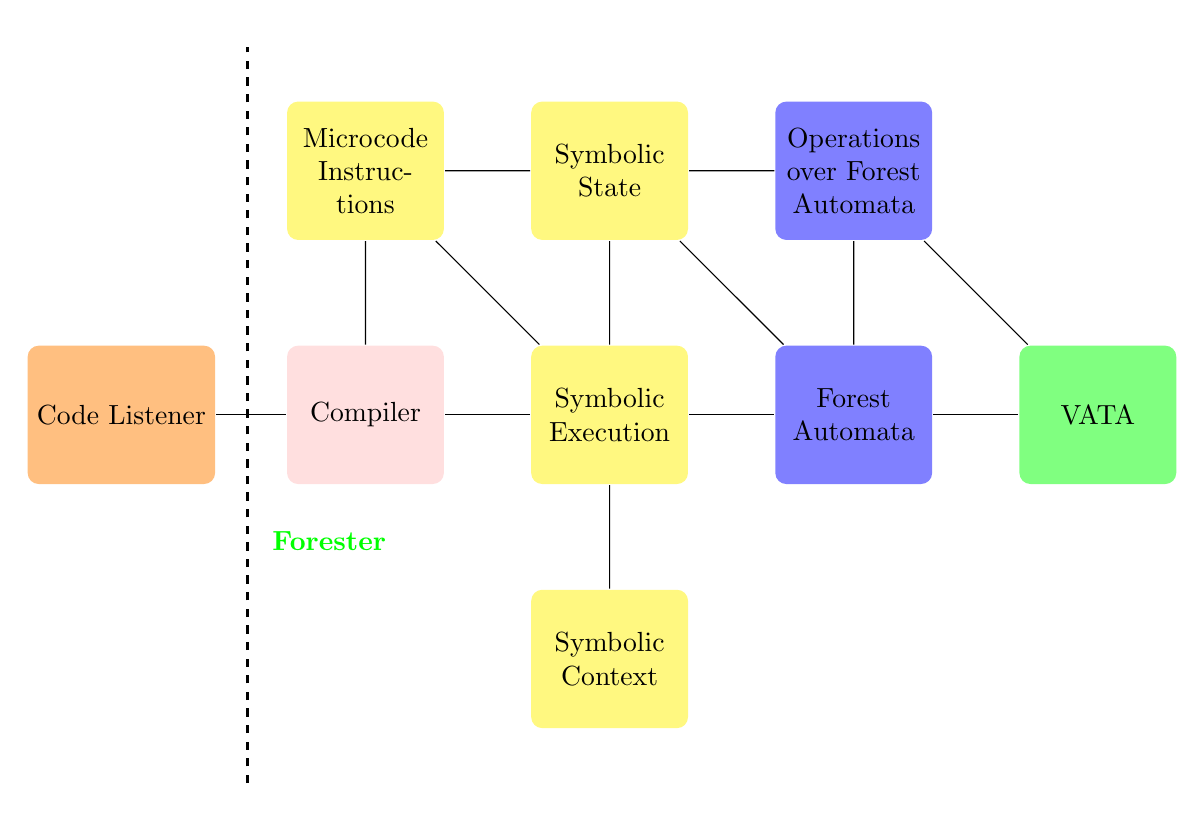
\begin{tikzpicture}[
  scale=0.8,
  node distance = 3.1cm,
  block_cl/.style={rectangle, text centered, rounded corners, thick, fill=orange!50,
    minimum height = 5em, minimum width = 3em},
  block_compiler/.style={rectangle, text centered, rounded corners, thick, fill=pink!50,
    minimum height = 5em, minimum width = 3em, text width = 5em},
  block_symex/.style={rectangle, text centered, rounded corners, thick, fill=yellow!50,
    minimum height = 5em, minimum width = 3em, text width = 5em},
  block_fa/.style={rectangle, text centered, rounded corners, thick, fill=blue!50,
    minimum height = 5em, minimum width = 3em, text width = 5em},
  block_ta/.style={rectangle, text centered, rounded corners, thick, fill=green!50,
    minimum height = 5em, minimum width = 3em, text width = 5em},
  line/.style={draw, -}
  ]

\node [block_cl] (cl) {Code Listener};
\node [block_compiler, right of=cl] (compiler) {Compiler};
\node [block_symex, above of=compiler] (microcode) {Microcode Instructions};
\node [block_symex, right of=compiler] (symex) {Symbolic Execution};
\node [block_symex, above of=symex] (symstate) {Symbolic State};
\node [block_symex, below of=symex] (symcnt) {Symbolic Context};

\node [block_fa, right of=symex] (fa) {Forest Automata};
\node [block_fa, above of=fa] (faop) {Operations over Forest Automata};

\node [block_ta, right of=fa] (ta) {VATA};

\path [line] (cl) -- (compiler);
\path [line] (microcode) -- (compiler);
\path [line] (symex) -- (compiler);
\path [line] (symex) -- (symstate);
\path [line] (symex) -- (symcnt);
\path [line] (symex) -- (fa);
\path [line] (symstate) -- (fa);
\path [line] (microcode) -- (symex);
\path [line] (fa) -- (faop);
\path [line] (fa) -- (ta);
\path [line] (symstate) -- (faop);
\path [line] (faop) -- (ta);
\path [line] (microcode) -- (symstate);

\node (LeftFAStart) at(2,-6) {};
\node (RightFAStart) at(2,6) {};
\draw [dashed, line width = 1pt] (LeftFAStart) -- (RightFAStart);
\node (Input) at(3.3,-2) {\textcolor{green}{\textbf{Forester}}};

\end{tikzpicture}

% 	\end{center}
% 	\caption{Conceptual design of \forester.}
% 	\label{fig:fa_design}
% \end{figure}

%Note, this is just the conceptual high level view of the Forester design.
% A~real implementation is much more complicated (e.g. Forest automata are implemented by two classes: \emph{FA} and \emph{FAE})
% and its full description is out of the scope of this chapter.

% %*******************************************************************************
% \vspace{-0.0mm}
% \subsection{Implementation of Forest Automata Concepts}
% \label{subsec:faimpl}
% \vspace{-0.0mm}
% %*******************************************************************************
%
% This section describes an implementation of the forest automata 
% based verification procedure in \forester.
% The core of the forest automata module is implemented by class {\tt FA}.
% This class stores an FA as a vector of tree automata $(t_1 \cdots t_n)$.
% Another data members of the class points to an automaton representing the global variables
% and to the automata representing the local variables of the actually executed function.
% The basic operations over an FA (like adding or removing a TA from an FA) are encapsulated in the class FA.
% The other class providing operations over FA is class {\tt FAE} (Forest Automata Extension). 
%
% The labels of the TA transitions are represented by the structure {\tt NodeLabel}.
% The structures is a tuple $\nodelab=(T,V)$ where $T$ determines the type of the root node of a transition
% (whether it is a general node, a data node or~a node containing a vector of data) and
% $V$ is a value of the type $T$ stored in the label.
%
% As it was already mentioned, the forest automata are further used to represent heap in symbolic states.
% An implementation of the representation of a symbolic state is in class {\tt SymState}.
% This class keeps a reference to a \forester microcode instruction $I$ executed at the~symbolic state.
% It has a data member that is a pointer to a forest automaton~$F$ (an instance of class {\tt FAE})
% representing the actual memory shape in the symbolic state.
% Another data member of class SymState is a set of registers $\regsset$.
% We denote set $\regsset$ by $\regs$.
%
% A~register can be local or global one.
% There are two global registers.
% The first one contains a reference to the forest automata modelling
% the global state, e.g., the block of global variables in the symbolic state.
% The other one represents a state of heap of the actually executed function.
% The local registers serve as temporary memory used in the microcode instructions for data manipulation.
% Putting together the data members of class {\tt SymState},
% we define symbolic state formally as a triple $S=\symstate{F}{\regs}{I}$.
%
% The values of the registers are instances of the structure {\tt Data}.
% We formally define structure Data as $\ddata$ where
% $T$ is a data type,
% $S \in \natnum$ is a size of data,
% $V$ is a value of type $T$,
% $\mathit{MB}=(D_1 \cdots D_n)$ are nested data for the case that $D$ is a data structure.
% The possible types $T$ are pointer, reference to a TA, integer, boolean, structure.
% $T$ can be also undefined or unknown type.
% We describe in detail one of the types\,---\,the root reference which is more structured.
% Its values are tuples $\rootref=(\rootit, \displ)$
% where $\rootit \in \natnum$ is an index of a tree automaton in $F$
% and the displacement $\displ \in \natnum$ is an index of a selector in a structured label
% under the root of the indexed tree automaton.
% Since the displacement $\displ$ is the sum of sizes of the preceding selectors
% it determines the precise position of the selector in label.
% The~operations for manipulation with a symbolic state are partially provided by class {\tt SymState}
% and some additional operations are provided by class {\tt VirtualMachine}.
%
% The symbolic execution is realized by gradually appending and removing the symbolic states from a queue.
% The implementation of symbolic execution is in class \emph{SymExec}.
% When a symbolic state is taken from the~queue, a microcode instruction contained in
% the symbolic state is executed.
% Some of the~instructions during its execution append a new symbolic state to the queue.
% Symbolic execution finishes when the queue is empty (or when an error is detected).
% The microcode instructions executed during the symbolic execution are described in the following section.

%*******************************************************************************
\subsection{\forester Microcode}\label{sec:microinstr}
%*******************************************************************************

In this section, we provide an example of \forester microcode.
Consider the following data structure implementing a~singly-linked list:
%
\begin{quote}
\begin{verbatim}
struct T {
  struct T* next;
  int data;
};
\end{verbatim}
\end{quote}
%
The syntax of a~microinstruction is $\mathit{op}\ r_0,\ r_1,\ r_2$
where $\mathit{op}$ is the name of an instruction and
$r_0, r_1$, and $r_2$ are operands such that $r_0$ is the destination register and
$r_1$ and $r_2$ are source registers or constants.
A~microinstruction can have zero to three operands.
The notation $[r+c]$ is used to access the selector with displacement~$c$ in a~label
under the root referenced by register~$r$.
% \bexmp\,
% 	The statement \codix{x = (struct\ \ T*)\ \ malloc(sizeof(struct\ \ T));} is translated
% 	to these microcode instructions:
% 	
% 	All constants used in the example are dependent on a concrete \forester
% 	run and they are chosen randomly in this text.
% 	The syntax of the microinstructions is $op\ r_0,\ r_1,\ r_2$
% 	where $op$ is a name of a instruction,
% 	$r_0, r_1, r_2$ are operands such that $r_0$ is a destination register and
% 	$r_1$ and $r_2$ are the source registers or constants.
%         All parameters are optional,
% 	$[r+c]$ is used to access the the selector with displacement $c$ in a label
%         under the root referenced by register $r$.
% \bexmp\,

Suppose that the verified program contains the following statement:
%
\begin{quote}
  % \codix{x = (struct\ \ T*)\ \ malloc(sizeof(struct\ \ T));}
\begin{verbatim}
x = malloc(sizeof(struct T));
\end{verbatim}
\end{quote}
%
The statement is translated into the following sequence of microinstructions:
%
\begin{quote}
\begin{verbatim}
1: mov_reg      r0, (int)8
2: alloc        r1, r0
3: node_create  r2, r1, <next,data>[0:4:+0,4:4:+0]
4: mov_reg      r3, ABP + 0
5: mov_reg      [r3 + 12], r2
6: check
\end{verbatim}
\end{quote}

First, on line~1, the size of the newly allocated data is stored into
register~$r_0$ (it is the size of \texttt{struct~T}, which is in this case~8).
Second, on line~2, a~new symbolic memory location of the size given by~$r_0$ is created
and its symbolic address stored into~$r_1$.
On line~3, we create a~new TA~$t$ with a~single transition representing
a~freshly created instance of the type \texttt{struct~T} at the memory location
give by~$r_1$ and append it to the FA representing the symbolic state.
The reference to the TA is stored into~$r_2$.
The type of the instance is given by \verb=<next,data>[0:4:+0,4:4:+0]=, which
gives names of the selectors and for each of them their offset (location in the memory cell),
size (we assumed a~32-bit system, which uses 4\,B for a~pointer, and~4\,B
\texttt{int}), and displacement (it is valid only for pointers and denotes offset
at which the pointer points into the referenced memory location%
\footnote{%
For instance, linked lists used within the Linux kernel do not point at the
beginning of the linked data structure, but, instead, into its middle (the position of
the \emph{list header}).
}).
On~line~4, a~reference to the TA representing the current function's stack frame
(ABP) is loaded into register~$r_3$.
(Note that in \forester, the program stack is represented using memory locations
on the heap.)
Finally, on line~5, the root reference to the TA~$t$ stored in register~$r_2$ is
added to the~selector with displacement~12 (corresponding to the displacement of
the local variable~\texttt{x} in the current stack frame) in the TA referenced
by register~$r_3$.
The instruction \texttt{check} on line~6 checks that the heap is garbage free.

% The TA $t$ has one transition with a label that consists of
% the pointer selector {\tt next} with displacement $0$ and size $4$.

% First, the size of the newly allocated data (in this case the size is $4$)
% is stored to the register $0$ at line~$1$.
% Then the new instance of the structure {\tt Data} is created and stored to register $0$ at line $2$.
% A~new TA $t$ is created at line $3$.
% The TA $t$ has one transition with a label that consists of
% the pointer selector {\tt next} with displacement $0$ and size $4$.
% The instruction \codix{node\_create} stores a root reference to $t$ to register $0$.
%       At line $4$, a reference to TA representing actual stack frame (ABP) is  loaded to register $r1$.
% Finally at line $5$, the root reference to $t$ stored in register $0$ is added to a selector with displacement $12$
%       in TA referenced by register $1$. Intuitively, the selector with displacement $12$ models memory pointed
%       by variable $x$.
% The instruction at line $6$ checks whether the heap is garbage-free.

% \eexmp


%%%%%%%%%%%%%%%%%%%%%%%%%%%%%%%%%%%%%%%%%%%%%%%%%%%%%%%%%%%%%%%%%%%%%%%%%%%%%%%%
\section{Tutorial}\label{sec:tutorial}
%%%%%%%%%%%%%%%%%%%%%%%%%%%%%%%%%%%%%%%%%%%%%%%%%%%%%%%%%%%%%%%%%%%%%%%%%%%%%%%%

\forester is can be obtained from its webpage \cite{foresterweb}, and the
easiest way to run it is from the virtual machine~\cite{zenodo}.
Once you boot the virtual machine (Ubuntu~16) you will find the \texttt{forester} folder
on the desktop.
The folder contains compiled binaries (the \texttt{fa\_build} folder) of \forester and also its source code (the \texttt{fa} folder).
For running the tool please read \texttt{README}.
The instruction for compilation of the tool are in the \texttt{INSTALL} file.

%*******************************************************************************
\subsection{Running \forester{} with BenchExec}
%*******************************************************************************

The BenchExec framework is a platform for evaluation of tools over a benchmark.
Since it is used for evaluation of the SV-COMP competition it contains modules necessary
for running \forester.
If you want to use BenchExec, you still need to compile \forester{} and provide the \texttt{include}
directory, the files \texttt{libfa.so}, and \texttt{sv\_comp\_run.py} from the directory \texttt{fa\_build}.
Please check the GitHub repository of BenchExec\footnote{\url{https://github.com/sosy-lab/benchexec/}} for further
information about how to run a tool using the framework.



%%%%%%%%%%%%%%%%%%%%%%%%%%%%%%%%%%%%%%%%%%%%%%%%%%%%%%%%%%%%%%%%%%%%%
\section{Experiments}\label{sec:exps}
% \vspace{-1.3mm}
%%%%%%%%%%%%%%%%%%%%%%%%%%%%%%%%%%%%%%%%%%%%%%%%%%%%%%%%%%%%%%%%%%%%%

The following section summarizes different experiments performed to evaluate
the abilities of~\forester{}.
The benchmark set consists of the tasks from~\cite{boxes13} and~\cite{vmcai17}.
We selected the programs in order to illustrate the two crucial features
of~\forester: the ability to learn boxes
automatically and counterexample analysis with abstraction refinement.
We also compare with \predator~\cite{predator11,dudka13sas}, a~many-times winner of
heap-manipulation-related categories of SV-COMP.

The benchmarks are C~programs manipulating singly and doubly-linked list, trees, skip lists, and their combinations.
We were able to analyse all of them fully automatically without any need to supply
manually crafted predicates or any other manual aid. The test cases are described in
detail in \secref{sec:testcases}.


%\begin{table}[bt]
%=======
%We implemented our method in \forester{}. The experiments were
%performed on a~PC with Intel Core i5@2.50 GHz CPU,
%8 GiB of memory, with Debian \texttt{sid} installed.
%Our benchmarks consist of programs manipulating singly- and
%doubly-linked list, and tree structures.
%We are able to analyse all the mentioned data
%structures fully automatically without the need to supply any manually crafted predicates.
%The benchmarks are in detail described in App.~\ref{sec:testcases}.

\begin{table}[t]
  % \vspace*{-2mm}
	\centering
	\scriptsize
	\caption{Results of experiments}
	\begin{tabular}{| l | l | r | r | r | r | r |}
        \hline
		Program & Status & LoC & Time [s] & Refnm& Preds & \predator [s]\\
        \hline
        \hline
        SLL (reverse)      & \safe & $32$ & $0.03$ & $0$ & $0$ & $0.03$ \\ \hline
        SLL (delete)       & \safe & $33$ & $0.02$ & $0$ & $0$ & $0.03$ \\ \hline
        SLL (insertsort)   & \safe & $36$ & $0.04$ & $0$ & $0$ & $0.03$ \\ \hline
        SLL (bubblesort)   & \safe & $42$ & $0.02$ & $0$ & $0$ & $0.2$  \\ \hline
        SLL (mergesort)    & \safe & $76$ & $0.08$ & $0$ & $0$ & $0.10$ \\ \hline
        DLL (reverse)      & \safe & $39$ &  $0.70$   & $0$  & $0$ & $0.03$ \\ \hline
        DLL (insert)       & \safe & $39$ &  $0.56$   & $0$  & $0$ & $0.05$ \\ \hline
        DLL (insertsort1)  & \safe & $47$ &  $0.40$   & $0$  & $0$ & $0.11$ \\ \hline
        DLL (insertsort2)  & \safe & $48$ &  $0.12$   & $0$  & $0$ & $0.05$ \\ \hline
        CDLL               & \safe & $32$ &  $0.02$   & $0$  & $0$ & $0.03$ \\ \hline
        SLL+head           & \safe & $33$ & $0.05$ & $0$ & $0$ & $0.03$ \\ \hline
        SLL-Linux          & \safe & $60$ & $0.03$ & $0$ & $0$ & $0.03$ \\ \hline
        DLL+subdata        & \safe & $40$ &  $0.12$   & $0$  & $0$ & $\infty$ \\ \hline
        SLLOfCSLL          & \safe & $47$ & $0.02$ & $0$ & $0$ & $0.05$ \\ \hline
        SLLOf2CDLL-Linux   & \safe & $35$ & $0.16$ & $0$ & $0$ & $0.26$ \\ \hline
        SkipList$_2$       & \safe & $84$ &  $3.36$   & $0$  & $0$ & $\infty$ \\ \hline
        SkipList$_3$       & \safe & $92$ &  $20.05$  & $0$  & $0$ & $\infty$  \\ \hline
        \rowcolor{rowgray} \textbf{SkipList$_2$} & \unsafe & $ 84$ & $0.08$  & $1$  & $1$ & $0.10$ \\ \hline
        \rowcolor{rowgray} \textbf{SLL01}       & \safe & $70$ & $0.90$   &  $1$  & $1$  & $err$ \\ \hline
        \rowcolor{rowgray} \textbf{DLL01}       & \safe & $73$ &  $0.54$  & $2$  & $2$  & $2.2$\\ \hline
        \rowcolor{rowgray} \textbf{CSLLMon} & \safe & $49$ & $2.1$   &  $3$  & $3$  & $2.3$ \\ \hline
        \rowcolor{rowgray} \textbf{CDLLMon} & \safe & $52$ &  $31.0$ & $18$ & $24$ & $2.3$\\ \hline
        \rowcolor{rowgray} \textbf{OptPtrSLL}   & \safe & $59$ & $0.94$   & $3$   & $3$  & $\infty$\\ \hline
        \rowcolor{rowgray} \textbf{OptPtrDLL}   & \safe & $62$ &  $1.3$  & $5$  & $5$  & $\infty$\\ \hline
        \rowcolor{rowgray} \textbf{QueueSLL}    & \safe & $71$ & $17.00$  &  $10$ & $10$ & $2.2$ \\ \hline
        \rowcolor{rowgray} \textbf{QueueDLL}    & \safe & $74$ &  $1.5$ & $14$ & $14$ & $2.1$\\ \hline
        \rowcolor{rowgray} \textbf{GBSLL}       & \safe & $64$ & $6.10$   &  $3$  & $3$  & $\infty$\\ \hline
        \rowcolor{rowgray} \textbf{GBDLL}       & \safe & $71$ &  $1.4$  & $4$  & $4$  & $\infty$\\ \hline
        \rowcolor{rowgray} \textbf{GBSLLSent}   & \safe & $68$ & $0.48$   &  $3$  & $3$  & $\infty$\\ \hline
        \rowcolor{rowgray} \textbf{GBDLLSent}   & \safe & $75$ &  $1.3$  & $4$  & $4$  & $\infty$\\ \hline
        \rowcolor{rowgray} \textbf{RGSLL}       & \safe & $72$ & $14.41$  &  $22$ & $38$ & $0.13$\\ \hline
        \rowcolor{rowgray} \textbf{RGDLL}       & \safe & $76$ &  $78.76$ & $26$ & $26$ & $0.13$\\ \hline
        \rowcolor{rowgray} \textbf{WBSLL}       & \safe & $62$ & $0.71$   &  $5$  & $5$  & $0.16$\\ \hline
        \rowcolor{rowgray} \textbf{WBDLL}       & \safe & $71$ &  $1.60$  & $7$  & $7$  & $0.14$\\ \hline
        \rowcolor{rowgray} \textbf{SortedSLL}   & \safe & $190$ & $227.12$ & $15$ & $15$ & $2.2$\\ \hline
        \rowcolor{rowgray} \textbf{SortedDLL}   & \safe & $82$ &  $120.00$ & $11$ & $11$ & $2.20$\\ \hline
        \rowcolor{rowgray} \textbf{EndSLL}      & \safe & $45$ & $0.10$    &  $2$  & $2$ & $2.1$\\ \hline
        \rowcolor{rowgray} \textbf{EndDLL}      & \safe & $49$ &  $0.14$  & $3$  & $3$  & $1.8$\\ \hline
        \rowcolor{rowgray} \textbf{TreeRB}      & \unsafe & $130$ &  $0.08$  & $0$  & $0$ & $\infty$\\ \hline
        \rowcolor{rowgray} \textbf{TreeWB}     & \unsafe & $125$ &  $0.05$  & $0$ & $0$ & $\infty$ \\ \hline
        TreeCnstr   & \safe & $52$  & $0.31$   & $0$  & $0$ & $\infty$\\ \hline
        \rowcolor{rowgray} \textbf{TreeCnstr}   & \unsafe & $52$  &  $0.03$  & $0$ & $0$ & $\infty$ \\ \hline
        TreeOfCSLL  & \safe & $109$ &  $0.57$  & $0$  & $0$ & $\infty$\\ \hline
        \rowcolor{rowgray} \textbf{TreeOfCSLL}  & \unsafe & $109$ & $0.56$  &  $1$ & $3$ & $\infty$ \\ \hline
        TreeStack   & \safe & $58$  &  $0.20$  & $0$  & $0$ & $\infty$\\ \hline
        \rowcolor{rowgray} \textbf{TreeStack}   & \unsafe & $58$  & $0.01$  & $0$ & $0$ & $\infty$ \\ \hline
        TreeDsw     & \safe & $72$  & $1.87$   & $0$  & $0$ & $\infty$\\ \hline
        \rowcolor{rowgray} \textbf{TreeDsw}     & \unsafe & $72$  & $0.02$  & $0$ & $0$ & $\infty$ \\ \hline
        TreeRootPtr & \safe & $62$  &  $1.43$  & $0$  & $0$ & $\infty$\\ \hline
        \rowcolor{rowgray} \textbf{TreeRootPtr} & \unsafe & $62$  & $0.17$  & $2$ & $6$ & $\infty$\\ \hline
	\end{tabular}
	\label{tab:times}
  % \vspace{-4mm}
  % \vspace{-8mm}
\end{table}

We present our experimental results in Table~\ref{tab:times}.
% The times in the table are averages of ten measurements (\forester{} chooses its path through ART nondeterministicaly, which can result in slightly variable execution times).
The table gives for each test case its name, the information whether the program is safe or
contains an error, the number of lines of code, the time needed for the analysis,
the number of refinements, the number of predicates learnt during
the abstraction refinement, and, finally, the time that \predator needed to
analyse it (\emph{err}~denotes a~wrong answer and $\infty$ denotes timeout,
which was set to 900\,s, the same as in SV-COMP).
%
% The experiments were
%performed on a~computer with Intel Core i5@2.50\,GHz CPU and
%8\,GiB of memory running the Debian Sid OS with the Linux kernel.

Some of the test cases consider dynamic data structures without any data stored
in them, while some of them consider data structures storing finite-domain data.
Such data can
be a~part of the data structure itself, as, e.g., in red-black trees; they can
arise from some finite data abstraction; or they are also sometimes used to
mark some selected nodes of the data structure when checking the way the data
structure is changed by a given algorithm (e.g., one can check whether an
arbitrarily chosen successive pair of nodes of a~list marked red and green is
swapped when the list is reversed---see e.g.~\cite{artmc}).

%As the results show, some of our test cases do not need the abstraction to be refined.
As the results show, some of our test cases do not need refinement.
This is because the predicate abstraction (even with the empty set of predicate
languages) is \emph{a priori} restricted in order to preserve the forest automata root interconnection graph (cf.\ \secref{sec:icgraph}),
which roughly corresponds to the reachability relation among variables and
cut-points in the heaps represented by a~forest automaton.
This restriction was already used with the
finite height abstraction in the versions of \forester
from~\cite{habermehl:forest,boxes13}.

Table~\ref{tab:times} also provides a comparison of the version of~\forester
from~\cite{boxes13} with the version from~\cite{vmcai17}.
In particular, the highlighted cases are not manageable by the version from~\cite{boxes13}.
These cases can be split into two classes.
In the first class, there are safe programs where the initial abstraction is too
coarse and introduces spurious counterexamples, and the abstraction thus needs
to be refined.
The other class consists of programs 
containing a~real error (which could not be confirmed without the backward run).
The times needed for analysis are comparable in both versions of \forester.

To illustrate a typical learnt predicate, let us consider the test case \mbox{\emph{GBSLL}}.
This program manipulates a list with nodes storing two data values, green and blue, for which it holds
that a~green node is always followed by a~blue one (this data structure is
a~simplified version of a~red-black tree).
The program also contains a tester code to test this property.
\forester{} first learns two predicate languages describing particular violations of the property:
(1)~``a~green node is at the end of the list'' and
(2)~``there are two green nodes in a~row.''
After that, \forester{} derives a~general predicate representing all lists with
the needed invariant, i.e, every green node is followed by a~blue one.
The program is then successfully verified. 
%The ability to learn shape as well as data properties (as well as properties
%relating shape with data) using a uniform mechanism is one the features of our
%method which distinguishes it from most of the related work.

Another example comes from the analysis of the program \emph{TreeOfCSLL}, which
creates and deletes a tree where every tree node is also the head of a~circular
singly-linked list.
%
The program contains an undefined pointer dereference error in the deletion of the
circular lists.
%
\forester{} first finds a spurious error (also an undefined pointer dereference)
in the code that creates the circular lists.
%
In particular, the abstraction introduces a case in which a tree node that is
also the head of a list needs not be allocated, and an attempt of accessing its
next selector causes an undefined pointer dereference error. 
%
This situation is excluded by the first refinement, after which the error within
the list deletion is correctly reported.
%
Notice that, in this case, the refinement learns a property of the shape, not a
property over the stored data values. 
%
% The ability to learn shape as well as data properties (as well as properties
% relating shape with data) using a uniform mechanism is one the features of our
% method which distinguishes it from most of the related work.
%
The ability to learn shape as well as data properties (as well as properties
relating shape with data) using a~uniform mechanism is one of the features of our
method that distinguishes it from most of the related work.


%%%%%%%%%%%%%%%%%%%%%%%%%%%%%%%%%%%%%%%%%%%%%%%%%%%%%%%%%%%%%%%%%%%%%
\subsection{Description of Benchmarks}\label{sec:testcases}
%%%%%%%%%%%%%%%%%%%%%%%%%%%%%%%%%%%%%%%%%%%%%%%%%%%%%%%%%%%%%%%%%%%%%

In this section, we describe the test cases used above in our experimental
evaluation.
% The list data structures in all examples have a pointer called \emph{next} pointing
% to the next node in the linked list.
Note that we use a limited set of integer values since we do not support
integer abstraction.
We use ``SLL'' and ``DLL'' to denote singly and doubly-linked lists
respectively.

The cases described in the following list satisfy some (regular-expressible)
safe invariant (if their status in the table is ``safe'') or contain an error
(if their status is ``error'').
As an error, we consider violation of memory safety properties, i.e.,  absence
of $\nil$/undefined pointer dereference, invalid free, and presence of garbage.
For some data structures, we have both a~safe case and an~error case.
%
\begin{itemize}
  \item \emph{(SLL/DLL) (operation)}: Performing \emph{operation} on a~SLL/DLL.
  \item \emph{CDLL}: Construction of a~circular DLL.
  \item \emph{SLL+head}: Construction of a~list where each element points to
    the head of the list.
  \item \emph{SLL-Linux}: Implementation of lists used in the Linux kernel,
    which uses type casts and restricted pointer arithmetic.
  \item \emph{DLL+subdata}: A DLL implementation that uses data pointers
    pointing either inside the list nodes or optionally outside of them.
  \item \emph{SLLOf(CSLL/2CDLL)}: An SLL of circular SLLs or two circular DLLs
    respectively.
  \item \emph{SkipList$_i$}: Construction and traversal of a~skip
    list of level~$i$.
  \item \emph{(SLL/DLL)01}: The nodes of the list may or may not point to
    an external node, which, if present, is unique for each list item.
    We check the invariant that each node has a pointer set to $\nil$ or
    to an address of an external node.
  \item \emph{C(SLL/DLL)Mon}: A circular SLL/DLL consisting of nodes with integer values.
    The head of the list has the reserved value~$0$. The rest of the nodes with their integer values
    form a~non-decreasing sequence. We verify that the successor of an arbitrary node
    can have a smaller value than the node only when the successor is the head of the list.
  \item \emph{OptPtr(SLL/DLL)}: Each node of the list has an integer value, a pointer to the next node,
    and an optional pointer to an external node. When constructing the list, an integer value of every node
    is chosen nondeterministically. When the integer value $0$ or $1$ is chosen, the optional pointer points
    to the node itself. On the other hand, when $2$ is chosen, a new external node is allocated and
    its address is assigned to the optional pointer. We verify the relation of
    integer values and optional pointers for all nodes of the list.
  \item \emph{Queue(SLL/DLL)}: We create a list with nodes containing the integers 0, 1, 2, and~3.
    The list can form sequences $0$, $01$, $012$, $0123^*$. A particular sequence is created
    during construction of the list nondeterministically. We remember which sequence was actually created
    by an auxiliary integer variable. Then we traverse the list and check that
    the sequence formed by the list corresponds to the value of the auxiliary variable.
  \item \emph{GB(SLL/DLL)}: We create a list containing green and blue nodes. The colors
    arbitrarily alternate but it holds that a green node is always followed by a~blue node.
  \item \emph{GB(SLL/DLL)Sent}: This case is similar to the previous one but instead of
    terminating the list with the $\nil$ value, the list is terminated using a~dedicated sentinel node.
  \item \emph{RG(SLL/DLL)}: The list contains an arbitrary prefix of white nodes,
    one red node followed by a green one, and an arbitrary suffix of white nodes.
    The list is reversed and it is checked whether the green node is followed by the red node.
  \item \emph{WB(SLL/DLL)}: Exactly one blue node is inserted into a list of white nodes
    of an arbitrary length. Then the list is traversed and it is checked that the number of blue
    nodes is one.
  \item \emph{Sorted(SLL/DLL)}: This test case contains a sorted list of nodes with integer values $0$ and $1$.
    A node with value $1$ is added at an arbitrary position that keeps the order of values of nodes in the list.
    Finally, it is checked that the values of nodes in the list are still ordered.
  \item \emph{End(SLL/DLL)}: The last element of the list has a special integer value.
  \item \emph{TreeRB}: We construct a red black tree and then go through the tree
    checking (regular) invariants of this data structure. The created tree has an arbitrary height,
    and the nodes may have both, one, or no child allocated. A transposition of nodes needed to
    preserve the data structure's invariants is done continuously during construction of the tree when a new node is added.
    This operation is complex since it requires relocation of nodes in several levels of trees.
    The nodes also need to have parent pointers to allow the transposition.
  \item \emph{TreeWB}: We construct a tree that has all nodes white except exactly one blue node.
    The blue node is at an arbitrary position. We traverse the tree and check
    that there is a~single blue node.
	% \item \emph{TreeWBAllPaths}: A tree with all nodes being white is constructed
	% 	nondeterministically. We transform the created tree to the form where
	% 	each path from the root to any leaf contains exactly one blue
	% 	node. The blue nodes are placed arbitrarily in the tree with respect to
	% 	the described invariant of the structure. Then we start an arbitrary number of
	% 	arbitrary walks from the root of tree to a leaf and check that each
	% 	of these walks contains exactly one blue node.
\end{itemize}

The following test cases from our benchmark are checked only for memory safety properties.
\begin{itemize}
	\item \emph{TreeCnstr}: The construction of an arbitrary binary tree.
	\item \emph{TreeOfCSLL}: We construct a binary tree where each node points to a circular SLL
		of an arbitrary length. Then we traverse the whole tree and all nested lists.
	\item \emph{TreeStack}: The construction of a binary tree, which is subsequently destroyed using stack
		implemented by an SLL.
	\item \emph{TreeDsw}: We construct a binary tree and perform the Deutsch-Schorr-Waite traversal.
	\item \emph{TreeRootPtr}: The construction and traversal of a binary tree with nodes containing root pointers.
\end{itemize}

%%%%%%%%%%%%%%%%%%%%%%%%%%%%%%%%%%%%%%%%%%%%%%%%%%%%%%%%%%%%%%%%%%%%%%%%%%%%%%%%
%\section{Participation in SV-COMP}
%%%%%%%%%%%%%%%%%%%%%%%%%%%%%%%%%%%%%%%%%%%%%%%%%%%%%%%%%%%%%%%%%%%%%%%%%%%%%%%%


%% %------------------------------------------------------------------------------
%% \vspace*{-2mm}
%% \section{Discussion and Future Work}
%% \vspace*{-1mm}
%% %------------------------------------------------------------------------------
%% 
%% Both the described forward and backward symbolic execution are quite fast.
%% % , and \forester{} scales well. 
%% We believe that the efficiency of the backward run (despite the need of computing expensive automata products) is to a large degree because it inverts unfolding (by folding). 
%% Backward run is therefore carried out with configurations encoded in a~compact folded form. 
%% 
%% \forester{} was not able to terminate on a few tree benchmarks.  
%% For a program manipulating a red-black tree using the rebalancing procedures, 
%% the initial forward run did not terminate.  
%% For another tree-based implementation of a set that includes a tester code checking full functional correctness, the CEGAR did not learn the right
%% predicates despite many refinements.
%% %
%% The non-termination of the forward run is probably related to the initial
%% restrictions of the predicate abstraction. Restricting the abstraction seems to be harmful especially in the case of tree structures. 
%% If the abstraction remembers unnecessary fine information about tree branches, the analysis will explore exponentially many variants of tree structures with different branches satisfying different properties.
%% %
%% The scenario where CEGAR seems to be unable to generalize is related to the splitting of the symbolic execution. The symbolic runs are then too specialised and CEGAR learns a large number of too specialised predicates from them (which are sometimes irrelevant to the ``real'' cause of the error). 
%% %
%% 
%% A closer examination and resolution of these issues is a part of our future
%% work. Allowing the abstraction more freedom is mostly an implementation issue,
%% although nontrivial to achieve in the current implementation of \forester{}.
%% Resolving the issue of splitting requires to cope with the domain of forest
%% automata not being closed under union. This is possible, e.g., by modifying the
%% definition of the FA language, which currently uses the Cartesian product of
%% sets of trees, so that it would connect tree components based on reachability
%% relation between them (instead of taking all elements of the Cartesian product).
%% Another possibility would be to use sets of forest automata instead of
%% individual ones as the symbolic representation of sets of heaps.  
%% 
%% %properties of refinement on the level of properties of the shape,
%% %not over the data. 



%%%%%%%%%%%%%%%%%%%%%%%%%%%%%%%%%%%%%%%%%%%%%%%%%%%%%%%%%%%%%%%%%%%%%
%\section{conclusions}
%%%%%%%%%%%%%%%%%%%%%%%%%%%%%%%%%%%%%%%%%%%%%%%%%%%%%%%%%%%%%%%%%%%%%

% \section{Related Work} 
% The area of verifying programs with dynamic linked
% data structures has been a subject of intense research for quite some time. Many
% different approaches based on logics, e.g.,
% \cite{pale01,pale,Reynolds:SepLogic:02,InvaderCAV07,indPrSynt07,ndqc07,Zee:pldi08,InvaderCAV08,abduction11,mpq11,slayer11,predator11,overlaid11,indPrSynt07,thor10,sas07:chang_rival_necula},
% automata \cite{bhrv06b,lists-counters,deg06}, graph grammars \cite{juggrnaut10,juggrnaut-learning12}, upward closed sets \cite{paroshBackward},
% and other formalisms have been proposed. These approaches differ in their
% generality, efficiency, and degree of automation.  
% %
% What makes our approach based on forest automata stand out is the combination of
% 1) high efficiency,
% 2) automation,
% 3) generality and complexity of the class of the shape graphs that the approach can handle in practice, and
% 4) the ability to analyse counterexamples and learn abstraction refinements from them.
%The closest lines of work to forest automata are \cite{bhrv06b}, that also uses automata, 
%the use of separation logic in the works \cite{InvaderCAV07,InvaderCAV08} linked with the Space Invader tool. 
%
%
%In fact, as
%is clear from the above, the approach we propose combines some features from
%these two lines of research.
% From the point of view of efficiency and degree of automation, the main
% alternative to our approach is the fully-automated use of separation logic with
% inductive list predicates as implemented in \spaceinvader~\cite{InvaderCAV08} or
% \slayer~\cite{slayer11}. These approaches are, however, much less general than
% our approach since they are restricted to programs over certain classes of
% linked lists (and cannot handle even structures such as linked lists with data
% pointers pointing either inside the list nodes or optionally outside of them,
% which we can easily handle, as discussed later on). 
% The work \cite{overlaid11} concerning overlaid data
% structures mentions an extension of \spaceinvader to trees, but this extension
% is of a limited generality and requires some manual help.
% A similar comparison applies
% to the \predator tool, which uses a~graph-based
% formalism~\cite{predator11} based on separation logic.
% In terms of generality of the handled class of shape graphs and automation,
% \cite{indPrSynt07}~and~\cite{locle:secondorder} are close to our work. 
% They can both handle some impressively complex data structures, even tree-like structures
% with additional pointers.
% For instance, the so-called mcf
% trees of~\cite{indPrSynt07}, which are trees whose nodes have an arbitrary number of successors
% linked in a~DLL, is even more general than what can in principle
% be described by hierarchically nested FAs (to describe mcf trees, recursively
% nested FAs or FAs based on hedge automata would be needed).
% On the other hand, both of these approaches are rather fragile. Especially~\cite{indPrSynt07}
% seems quite dependent on the fact that the encountered
% data structures are built in a ``nice'' way conforming to the structure of the
% predicate to be learnt (meaning, e.g., that lists are built by adding elements
% at the end only), which is close to providing an inductive definition of the
% data structure, and, similarly, \cite{locle:secondorder}~fails on examples that
% might seem easy (such as certain rather straightforward variants of creations
% and deletions of a~doubly-linked list).
% %
% Counterexample analysis is also problematic for both of them and it is not clear
% whether they would be amenable for some kind of abstraction refinement.
% %
% The grammar-based encoding of heaps from~\cite{juggrnaut10} is conceptually close to forest automata and separation logic, and has a similar potential.
% A concept of inferring graph grammar rules for the heap abstraction proposed
% in~\cite{juggrnaut10} has appeared in~\cite{juggrnaut-learning12}.
% %
% The proposed technique can so far only handle less general structures than our
% approach though.
% 
% We note that there
% are other works on separation logic, e.g.~\cite{ndqc07}, that consider tree
% manipulation, but these are usually semi-automated only. 
% %
% The work \cite{thor10} proposes an approach that uses separation logic for
% generating numerical abstractions of heap manipulating programs allowing for
% checking both their safety as well as termination. The described experiments
% include even verification of programs with 2-level skip lists.
% The work, however,
% still expects the user to manually provide an inductive definition of skip lists
% in advance. Likewise, the work \cite{sas07:chang_rival_necula} based on the so-called separating
% shape graphs reports on verification of programs with 2-level skip lists, but it
% also requires the user to come up with summary edges to be used for summarizing
% skip list segments, hence basically with an inductive definition of skip lists.
%Compared to \cite{thor10,sas07:chang_rival_necula}, we did not have to provide any manual aid
%whatsoever to our technique when dealing with 2-level as well as 3-level
%skip lists in our experiments.
% 
% A common weakness of the
% current approaches to shape analysis such as \cite{InvaderCAV07,InvaderCAV08,indPrSynt07,locle:secondorder,predator11,slayer11,juggrnaut10,juggrnaut-learning12} is a lack of proper support for checking
% spuriousness of counterexample traces and automated refinement
% of the employed abstraction (as noted also in~\cite{splinter15}).
% %
% An example of a~program that the mentioned approaches cannot handle is a~program
% dealing with lists of lists where the sub-lists are of
% length 0 or 1, which is a quite practical situation~\cite{InvaderTR07}. In such
% cases, the abstraction used in \cite{InvaderCAV07,InvaderCAV08} can fail,
% leading to an infinite computation (e.g., when, by chance, a list of regularly
% interleaved lists of length 0 or 1 appears) or generate false alarms (when
% modified to abstract even pointer links of length 1 to a list segment). For us,
% such a~situation is easy to handle without any need to fine-tune the abstraction
% manually. 
% %
% %
% %Our approach combines a use of our nested FA with an  automatically
% %refinable abstraction on the TA that appear in our representation. Thus our
% %analysis can more easily adjust to various cases arising in the programs being
% %verified.
% %
% %
% A number of works have attempted to remedy this weakness.
% %%%%%%%%%%%%%%%%%%%%%%%%%
% The work \cite{beyer:lazy_shape_analysis} adds a CEGAR loop on top of the TVLA
% analyzer \cite{pale}, which is based on \emph{3-valued predicate logic with
% transitive closure}. 
% %
% The work
% \cite{Loginov:AbstrRefViaInductLearning:05} also builds on TVLA but goes
% further by learning more complex instrumentation relations using
% inductive logic programming.
% %
% In \cite{podelski:popl10}, a CEGAR-based approach was proposed for automated
% refinement of the so-called \emph{Boolean heap abstraction} using disjunctions
% of universally quantified Boolean combinations of first-order predicates with
% free variables and transitive closure.
% %
% Among separation-logic-based approaches, the works~\cite{slayer12,splinter15,botincan15} 
% also feature different kinds of counterexample analysis and/or abstraction refinement.
% %
% None of these works, however, achieves the degree of automation, generality, or
% precision of the counterexample analysis and flexibility of the abstraction
% learning mechanism as our forest-automata-based approach.
%
%%%%%%%%%%%%%%%%%%%%%%%%%%
%
%Finally, compared with~\cite{bhrv06b}, our newly proposed approach is a~bit less
%general. We cannot handle structures such as, e.g., trees with linked leaves. To
%handle these structures, we would have to introduce into our approach FA nested
%not just strictly hierarchically but in an arbitrary, possibly cyclic way, which
%is an interesting subject for future research. On the other hand, our new
%approach is more scalable than that of \cite{bhrv06b}. This is due to the fact
%that the heap representation in \cite{bhrv06b} is monolithic, i.e., the whole
%heap is represented by a single tree skeleton over which additional pointer
%links are expressed using the so-called routing expressions. The new encoding is
%much more structured, and so the different operations on the heap, corresponding
%to a~symbolic execution of the verified program, typically influence only small
%parts of the encoding and not all (or most) of it. The monolithic encoding of
%\cite{bhrv06b} has also problems with deletion of elements inside data
%structures since the routing expressions are built over a~tree backbone that is
%assumed not to change (and hence deleted elements inside data structures are
%always kept, just marked as deleted). Moreover, the encoding of~\cite{bhrv06b}
%has troubles with detection of memory leakage, which is in theory possible, but
%it is so complex that it has never been implemented. 
%
%Lastly, among \emph{automata-based approaches}, counterexample analysis and
%refinement was used in \cite{bhrv06b} (and also in some related less general
%approaches like~\cite{bhmv05}). In that case, however, a single tree automaton
%was used to encode sets of memory configurations, which allowed standard
%abstraction refinement from abstract regular (tree) model checking
%\cite{artmc} to be used. On the other hand, due to using a single automaton,
%the approach did not scale well and had problems with some heap transformations.
% 
% This paper is based on earlier published works on forest automata \cite{habermehl:forest} and SVComp contributions \cite{},
% mainly on \cite{habermehl:forest} for the overall overview and on \cite{holik:cexfa,jiri:diza} for the technical part.
% It does not comprise the works on verification of properties of data stored in forest automata \cite{forester-data-acta} and 
% an advanced algorithms for learning boxes \cite{holik:automated}.
\begin{comment}
\chapter{Forester VMCAI}
\label{ch:vmcai}
%%%%%%%%%%%%%%%%%%%%%%%%%%%%%%%%%%%%%%%%%%%%%%%%%%%%%%%%%%%%%%%%%%%%%
\section{Introduction}\label{sec:label}
%%%%%%%%%%%%%%%%%%%%%%%%%%%%%%%%%%%%%%%%%%%%%%%%%%%%%%%%%%%%%%%%%%%%%

In~\cite{forester12,boxes13}, \emph{forest automata} (FAs) were proposed as a
formalism for representing sets of heap graphs within a fully-automated and
scalable \emph{shape analysis} of programs with complex \emph{dynamic linked
data structures}. FAs were implemented in the \forester{} tool and successfully
used to verify programs over a wide range of data structures, such as different
kinds of lists (singly- and doubly-linked, circular, nested, and/or having
various additional pointers), different kinds of trees, as well as skip lists.
FAs have the form of tuples of \emph{tree automata} (TAs), allowing abstract
transformers corresponding to heap operations to have a \emph{local impact}
(i.e., to change just a few component TAs instead of the entire heap
representation), leading to scalability. To handle complex nested data
structures, FAs may be \emph{hierarchically nested}, i.e., lower-level FAs can
be used as (automatically derived) alphabet symbols of higher-level FAs.

Despite \forester{} managed to verify a number of programs, it suffered from two
important deficiencies.
Namely, due to using abstraction and the lack of
mechanisms for checking validity of possible counterexamples, it could report
\emph{spurious errors}, and, moreover, it was unable to refine the abstraction
using the spurious counterexample.
% Despite \forester{} managed to verify a number of programs, it suffered from one
% important deficiency. Namely, due to using abstraction, it could report
% \emph{spurious errors},
% but it lacked a mechanism for checking validity of
% possible counterexamples as well as a mechanism for a counterexample-guided
% refinement of the abstraction used.
Interestingly, as discussed in the related
work section, this problem is common for many other approaches to shape
analysis, which may perhaps be attributed to the complexity of heap
abstractions. In this paper, we tackle the above problem by providing a novel
method for \emph{validation of possible counterexample traces} as well as a
\emph{counterexample guided abstraction refinement} (CEGAR) loop for shape
analysis based on FAs.

%!!!!!!!!!!!!!!!!!!!!!!!!!!!!!!!!!!!
%!!!!!!!!!!!!!!!!!!!!!!!!!!!!!!!!!!!

Our counterexample validation is based on \emph{backward symbolic execution} of
a candidate counterexample trace on the level of FAs (with no abstraction on the
FAs) while checking \emph{non-emptiness of its intersection} with the forward
symbolic execution (which was abstracting the FAs). For that, we have to revert
not only abstract transformers corresponding to program statements but also
various meta-operations that are used in the forward symbolic execution and that
significantly influence the way sets of heap configurations are represented by
FAs. In particular, this concerns \emph{folding} and \emph{unfolding} of nested
FAs (which we call \emph{boxes}) as well as \emph{splitting}, \emph{merging},
and \emph{reordering} of component TAs, which is used in the forward run for the
following two reasons: to
prevent the number of component TAs from growing and to obtain a canonic
FA representation. 

If the above meta-operations were not reverted, we would not only have problems
in reverting some program statements but also in intersecting FAs obtained from
the forward and backward run. Indeed, the general problem of checking emptiness
of intersection of FAs that may use different boxes and different component TAs
(i.e., intuitively, different decompositions of the represented heap graphs) is
open. When we carefully revert the mentioned operations, it, however, turns out
that the FAs obtained in the forward and backward run use \emph{compatible}
decomposition and hierarchical structuring of heap graphs, and so checking
emptiness of their intersection is possible. Even then, however, the
intersection is not trivial as the boxes obtained in the backward run may
represent smaller sets of sub-heaps, and hence we cannot use boxes as symbols
and instead have to perform the intersection \emph{recursively} on the boxes as
well.

Our abstraction on FAs is a modification of the so-called \emph{predicate
language abstraction} \cite{artmc}.
This particular abstraction collapses those states of component TAs that
have non-empty intersection with the same predicate languages, which are
obtained from the backward execution.
We show that, in
case the intersection of the set of configurations of the above described forward and backward symbolic runs
is empty, we can derive from it an \emph{automata interpolant} allowing us to
get more predicate languages and to refine the abstraction such that progress of
the CEGAR loop is guaranteed (in the sense that  we do not repeat the same
abstract forward run).

We have implemented the proposed approach in \forester{} and tested it on a
number of small but challenging programs. Despite there is, of course, a lot of
space for further optimisations, the experimental results are 
% 
% simply amazing (no need to be unnecessarily humble).
%
very encouraging.
%
\forester{} can now not only verify correct programs with complex dynamic data
structures but also reliably report errors in such programs. For some classes of
dynamic data structures (notably skip lists), \forester{} is, to the best of our
knowledge, the only tool that can provide both sound verification as well as
reliable error reporting in a fully automated analysis (i.e., no manually
provided heap predicates, no invariants, etc.). Moreover, for some classes of
programs (e.g., various kinds of doubly-linked lists, trees, and nested lists),
the only other tool that we are aware to be able to provide such functionality
is our older automata-based tool \cite{bhrv06b}, which is, however, far less
scalable due to the use of a~monolithic heap encoding based on a single TA. Finally,
the refinement mechanism we introduced allowed us to verify some programs that
were before out of reach of \forester{} due to handling finite domain data
stored in the heap (which can be used by the programs themselves or introduced
by tagging selected elements in dynamic data structures when checking properties
such as sortedness, reordering, etc.).

%!!!!!!!!!!!!!!!!!!!!!!!!!!!!!!!!!!!
%!!!!!!!!!!!!!!!!!!!!!!!!!!!!!!!!!!!

%%%%%%%%%%%%%%%%%%%%%%%%%%%%%%%%%%%%%%%%%%%%%%%%%%%%%%%%%%%%%%%%%%%%%
%\section{Related Work}
%%%%%%%%%%%%%%%%%%%%%%%%%%%%%%%%%%%%%%%%%%%%%%%%%%%%%%%%%%%%%%%%%%%%%
%
%Many different approaches to shape analysis have been proposed, using various
%underlying formalisms, such as logics
%\cite{jensen,pale,InvaderCAV08,thor10,dragoi:atva12,sleek13}, automata
%\cite{bhrv06b,deg06,forester12,boxes13,lists-counters}, graphs
%\cite{sas07:chang_rival_necula,dudka13sas}, or graph grammars \cite{juggrnaut10}.
%Apart from the underlying formalisms, the approaches differ in their degree of
%automation, in the heap structures they can handle, and in their scalability.
%The shape analysis based on forest automata proposed in \cite{boxes13} that we
%build on in this paper belongs among the most general, fully automated
%approaches, still having decent scalability.
%
%As noted also in the recent work \cite{splinter15}, a common weakness of the
%current approaches to shape analysis is a lack of proper support for checking
%spuriousness of counterexample traces, possibly followed by automated refinement
%of the employed abstraction. This is exactly the problem that we tackle in this
%paper. Below, we characterize previous attempts on the problem and compare our
%approach with them. 
%
%The work \cite{beyer:lazy_shape_analysis} adds a CEGAR loop on top of the TVLA
%analyzer \cite{pale}, which is based on \emph{3-valued predicate logic with
%transitive closure}. The refinement is, however, restricted to adding more
%pointer variables and/or data fields of allocated memory cells to be tracked
%only (together with combining the ana\-ly\-sis with classic predicate analysis on
%data values). The analysis assumes the other necessary heap predicates (i.e.,
%the so-called core and instrumentation relations in terms of \cite{pale}) to
%be fixed in advance and not refined. The work
%\cite{Loginov:AbstrRefViaInductLearning:05} also builds on TVLA but goes
%further by learning more complex instrumentation relations using
%inductive logic programming. The core relations are still fixed in
%% further by allowing more complex instrumentation relations to be learnt using
%% inductive logic programming. The core relations are, however, still fixed in
%advance though. Compared with both of these works, we do not assume any predefined
%fixed predicates. Moreover, the approach of
%\cite{Loginov:AbstrRefViaInductLearning:05} is not CEGAR-based---it refines the
%% abstraction whenever it hits a~possible counterexample trace in whose analysis
%abstraction whenever it hits a~possible counterexample in which
%some loss of precision happened, regardless of whether the counterexample is
%real or not.
%
%In \cite{podelski:popl10}, a CEGAR-based approach was proposed for automated
%refinement of the so-called \emph{Boolean heap abstraction} using disjunctions
%of universally quantified Boolean combinations of first-order predicates with
%free variables and transitive closure.
%%
%% The work uses CEGAR to both add new predicates and to refine the abstract post
%% operator. 
%%
%Unlike our work, the approach assumes the analyzed programs to be annotated by
%procedure contracts and representation invariants of data structures. New
%predicates are inferred using finite-trace weakest preconditions on the
%annotations, and hence new predicates with reachability constraints can only be
%inferred via additional heuristic widening on the inferred predicates. Moreover,
%the approach is not appropriate for handling nested data structures, such as
%lists of lists, requiring nested reachability predicates.
%
%%!!!!!!!!!!!!!!!!!!!!!!!!!!!!!!!!!!!
%%!!!!!!!!!!!!!!!!!!!!!!!!!!!!!!!!!!!
%
%In the context of approaches based on \emph{separation logic}, several attempts
%to provide counterexample validation and automated abstraction refinement have
%appeared. In \cite{slayer12}, the \textsc{SLAyer} analyzer was extended by a method to
%check spuriousness of counterexample traces via bounded model checking and SMT.
%Unlike our work, the approach may, however, fail in recognising that a given
%trace represents a real counterexample. Moreover, the associated refinement can
%only add more predicates to be tracked from a pre-defined set of such
%predicates. In \cite{splinter15}, another counterexample analysis for the
%context of separation logic was proposed within a computation loop based on the
%Impact algorithm \cite{impact06}. The approach uses bounded backwards abduction
%to derive so-called spatial interpolants and to distinguish between real and
%spurious counterexample traces. It allows for refinement of the predicates used
%but only by extending them by data-related properties. The basic predicates
%describing heap shapes are provided in advance and fixed. Another work based on
%backwards abduction is \cite{botincan15}. The work assumes working with a
%parametrized family of predicates, and the refinement is based on refining the
%parameter. Three concrete families of this kind are provided, namely,
%singly-linked lists in which one can remember bigger and bigger multisets of
%chosen data values, remember nodes with certain addresses, or track ordering
%properties. The basic heap predicates are again fixed. The approach does not
%guarantee recognition of spurious and real counterexamples nor progress of the
%refinement.
%
%Unlike our approach, none of the so-far presented works is based on automata,
%and all of the works require some fixed set of shape predicates to be provided
%in advance. Among \emph{automata-based approaches}, counterexample analysis and
%refinement was used in \cite{bhrv06b} (and also in some related, less general
%approaches like \cite{bhmv05}). In that case, however, a single tree automaton
%was used to encode sets of memory configurations, which allowed standard
%abstraction refinement from abstract regular (tree) model checking
%\cite{artmc} to be used. On the other hand, due to using a single automaton,
%the approach did not scale well and had problems with some heap transformations.
%
%% Finally, the Predator analyzer \cite{php15} avoids spurious errors by running a
%% sound, over-approximating analysis together with a precise one, allowing only
%% the latter to report counterexamples. This does not, however, allow the
%% abstraction used to be refined, possibly preventing correct programs from being
%% verified.
%
%The basic formalism of forest automata using fixed abstraction and
%user-provided database of boxes was introduced in~\cite{forester12}.
%We later extended the basic framework with automatic learning of boxes
%in~\cite{boxes13}.
%The work~\cite{forester-data-acta} added ordering relations into forest
%automata to allow verification of
%programs whose safety depends on relations among data values
%from an unbounded domain.
%In \cite{forester12,boxes13}, we conjectured that counterexample validation and
%abstraction refinement should be possible in the context of forest
%automata too. However, only now, do we show that this is indeed the case, but also that much
%more involved methods than those of \cite{artmc} are needed.
%
%%%%%%%%%%%%%%%%%%%%%%%%%%%%%%%%%%%%%%%%%%%%%%%%%%%%%%%%%%%%%%%%%%%%%
\section{Forest Automata and Heaps}
%%%%%%%%%%%%%%%%%%%%%%%%%%%%%%%%%%%%%%%%%%%%%%%%%%%%%%%%%%%%%%%%%%%%%

% \td{OL: talk only about heaps}

We consider sequential non-recursive C programs, operating on a set of pointer
variables and the heap, using standard statements and control flow constructs.
%Variables are either \emph{data variables} or \emph{pointer variables}.
Heap cells contain zero or several pointer or data fields.
%(our framework and implementation extends easily to several data fields).
% \comment[mh]{Why do you speak about commands here?}
%The supported statements include allocation and deallocation of heap memory,
%tests between data variables or fields of heap cells, as well as assignments
%between data variables, pointer variables, or fields of heap cells.

%\begin{figure}
%% \vspace{10mm}
%% \hspace{-4mm}
%\begin{center}
%\begin{tikzpicture}[%
%  codeblock/.style={text width=0.4\linewidth,rounded corners,inner xsep=12pt,inner ysep=0pt,below right,draw=gray!3!white},%
%  property/.style={rounded corners=1pt,inner xsep=1mm,draw=black!50,fill=white,double}%
%  ]
%  \node[codeblock] (code) {\small\VerbatimInput{code.txt}};
%\end{tikzpicture}%
%\end{center}
%\vspace*{-1mm}
%\caption{A function which inserts a~new node into a BST and returns a~pointer to
%its root node.}
%\label{fig:bst-code}
%\end{figure}
%
%Fig.~\ref{fig:bst-code} shows an example of a C function inserting a new node
%into a~BST (recall that in BSTs, the data value in a node is larger than all
%the values of its left subtree and smaller than all the values of its right
%subtree). Variable $\code{x}$ descends the BST to find the position at which
%the node $\code{newNode}$ with a new data value $\code{d}$ should be inserted.

Configurations of the considered programs consist of
memory-allocated data and an assignment of variables.
\emph{Heap memory} can be viewed as a~(directed) graph whose nodes correspond
to allocated memory cells.
Every node contains a~set of named pointer and data fields.
Each pointer field points to another node (we model the
$\code{NULL}$ and undefined locations as special memory nodes pointed by variables
$\code{NULL}$ and $\code{undef}$, respectively), and the same holds for pointer variables of the program.
Data fields of memory nodes hold a data value.
We use the term \emph{selector} to talk both about pointer and data fields.
For simplification, we model data variables as pointer variables pointing to
allocated nodes that contain a single data field with the value of the
variable, and therefore consider only pointer
variables hereafter.
%In our terminology, a~\emph{heap} consists of a~heap memory and mapping of
%(pointer) variables to memory nodes.

%% We represent heap memory as a~composition of trees as follows. We first identify the
%% \emph{cut-points} of the heap, i.e., nodes that are either referenced by a
%% pointer variable or by several selectors. We then split the heap into
%% (cut-point-free) tree
%% components such that each cut-point becomes the root of a tree component. To
%% represent the interconnection of tree components, we introduce a set of
%% \emph{root references}, one for each tree component. After decomposition of the
%% heap, selectors and variables that point to cut-points in the heap are redirected to
%% point to the corresponding root references. Such a tuple of tree components
%% (together with the mapping of variables) is called a~\emph{forest}.
%% The decomposition of a~heap into tree components can be
%% performed canonically as described at the end of Section~\ref{sec:fa}.

We represent heap memory by partitioning it into a~tuple of trees, the
so-called \emph{forest}.
The leaves of the trees contain information about roots of which trees they should be merged with to recover the original heap. 
Our \emph{forest automata} symbolic representations of sets of heaps is based
on representing sets of forests using tuples of tree automata.
%

% \td{OL: keep the example? START}
% \td{OL: maybe substitute with Fig.~\ref{fig:forest_rep}?}
% Fig.~\ref{fig:bst-graph}(a) shows a possible heap of the program in
% Fig.~\ref{fig:bst-code}. Nodes are shown as circles, labeled by their data
% values. Selectors are shown as edges. Each selector points either to a~node or
% to $\nullconst$ (denoting \texttt{NULL}). Some nodes are labeled by a~pointer
% variable that points to them. The node with data value $15$ is a cut-point since
% it is referenced by variable $\code{x}$. Fig.~\ref{fig:bst-graph}(b) shows a
% tree decomposition of the graph into two trees, one rooted at the node
% referenced by $\code{root}$, and the other rooted at the node pointed by
% $\code{x}$. The $\code{right}$ selector of the root node in the first tree
% points to root reference $\rr{2}$ ($\rr{i}$ denotes a reference to the $i$-th
% tree $\tree_i$) to indicate that in the graph, it points to the corresponding
% cut-point.
% \td{OL: keep the example? END}

%%% kicked out for the submission
%%% Fig.~\ref{fig:forest_rep_graph} shows an example of a~(data-free) heap;
%%% nodes are shown as circles, selectors are shown as edges.
%%% Each selector points either to a~node or to $\nullconst$ (denoting
%%% an edge to the \texttt{NULL} node).
%%% Some nodes are labeled by a~pointer variable that points to them.
%%% The nodes labelled with 1 and 3 are cut-points because they are pointed by
%%% variables (\texttt{x} and \texttt{y} respectively) and the node labelled with 2
%%% is a cut-point because it has two incoming edges.
%%% Fig.~\ref{fig:forest_rep_forest} shows a~forest representation of the heap from
%%% Fig.~\ref{fig:forest_rep_graph}.

Let us now formalize these ideas.
% \lukas{formulation sounds as it was a part of contribution, which it is not}
%  We will define heaps as parameterized by
% a~set $\abcd$ of selectors.
% E.g., when representing heaps, $\leaflab$ will contain the special value
% $\nullconst$; in tree components, $\leaflab$ will also include root references.
In the following, we use $f: A \partialto B$ to denote a partial function from
$A$ to $B$ (also
viewed as a~total function $f: A \to (B \cup \set{\top})$, assuming that $\top
\not\in B$).
We also assume a bounded data domain $\dset$. 
% \lukas{unbounded data domain frmo ACTA replaced by bounded data domain}
%with a total ordering
%relation $\preceq$.

% \begin{figure}[t]
%   \begin{minipage}[b]{5.6cm}
%     \centering
%     \vspace{-2mm}
%     \input{figs/bst_graph.tex}
%
%     \vspace{-1mm}
%     \small (a) A~graph.
%   \end{minipage}
%   \begin{minipage}[b]{6.8cm}
%     \begin{minipage}[t]{2.8cm}
%       \input{figs/bst_forest.tex}
%     \end{minipage}
%     \hspace{-0.0cm}
%     \begin{minipage}[t]{1.5cm}
%       \input{figs/bst_tree.tex}
%     \end{minipage}
%
%     \vspace{-1mm}
%     \centering
%    \small (b) A forest decomposition.
%   \end{minipage}
%   \vspace{-1mm}
%   \caption{Decomposition of a graph into trees.}
% \label{fig:bst-graph}
% \end{figure}

%% kicked out for the first submission
%% \begin{figure}[t]
%%   \begin{subfigure}[b]{0.48\textwidth}
%%   \centering
%%   \input{figs/fa-tree-decomp-graph.tikz}
%%   \caption{A~heap}
%%   \label{fig:forest_rep_graph}
%%   \end{subfigure}
%%   \hfill
%%   \begin{subfigure}[b]{0.48\textwidth}
%%   \centering
%%   \input{figs/fa-tree-decomp-forest.tikz}
%%   \caption{Its forest representation}
%%   \label{fig:forest_rep_forest}
%%   \end{subfigure}
%% \caption{A~heap and its forest representation.  For simplification, edges to
%% the dedicated $\nil$ node are represented using $\nullconst$ (we omit the
%% node from the graphical representation).}
%% \label{fig:forest_rep}
%% \end{figure}

%\bigskip
%\lukas{throw away $\leaflab$ completely? We can assume that $\abcd$ does not intersect with $\{\bar i\mid i\in\nat\}$ and use trees over $\abcd\cup\{\bar 1\,\ldots\bar n\}$ It looks like the only instantiation of $\leaflab$ is the $\{\bar 1,\ldots,\bar n\}$ anyway.}

%!!!!!!!!!!!!!!!!!!!!!!!!!!!!!!!!!!!
%!!!!!!!!!!!!!!!!!!!!!!!!!!!!!!!!!!!

%------------------------------------------------------------------------------
\paragraph{Graphs and Heaps.}
%------------------------------------------------------------------------------

Let $\abcd$ be a finite set of \emph{selectors} and $\leaflab$ be a~finite set
of \emph{references} s.t.~$\leaflab \cap \dset = \emptyset$.
A~\emph{graph}~$\graph$ over $\tuple{\abcd,\leaflab}$ is
% A~\emph{graph}~$\graph$ over $\abcd$ is
a tuple $\tuple{\nodesof{\graph},\selmapof{\graph}}$ where
$\nodesof{\graph}$ is a~finite set  of \emph{nodes} and $\selmapof{\graph}: \abcd \to (\nodesof{\graph}
\partialto (\nodesof{\graph}\cup \leaflab \cup \dset))$ maps each selector $a \in \abcd$
to a~partial mapping $\selmapof{\graph}(a)$ from nodes to nodes, references, or
data values.
%
References and data values are treated as special terminal
nodes that are not in the set of regular nodes, i.e., $V_g \cap (\leaflab \cup
\dset) = \emptyset$.
%
For a~graph~$\graph$, we use $\nodesof \graph$ to denote the nodes of~$\graph$,
and for a selector $a \in \abcd$, we
use $\selof{\graph}$ to denote the mapping $\selmapof{\graph}(a)$.
Given a finite set of variables~$\gvars$,
a~\emph{heap}~$\heap$ over $\tuple{\abcd, \gvars}$ is
a tuple $\tuple{\nodesof{\heap},\selmapof{\heap}, \asgnheap}$ where
$\tuple{\nodesof{\heap}, \selmapof{\heap}}$ is a~graph over $\tuple{\abcd,
\emptyset}$ and $\asgnheap: \gvars \to \nodesof{\heap}$ is a~(total)
map of variables to nodes.

% Let $\abcd$ be a finite set of {\em selectors} and $\leaflab$ be a~finite set
% of \emph{references}.  A~\emph{graph}~$\graph$ over $\tuple{\abcd,\leaflab}$ is
% a tuple $\tuple{\nodesof{\graph},\selmapof{\graph},\datmapof{\graph}}$ where
% $\nodesof{\graph}$ is a~finite set  of \emph{nodes} (assuming $\nodesof{\graph}
% \cap \leaflab = \emptyset$), $\selmapof{\graph}: \abcd \to (\nodesof{g}
% \partialto (\nodesof{\graph} \cup \learlab))$ maps each selector $a \in \abcd$
% to a partial mapping $\selmapof{\graph}(a)$ from nodes to nodes and references,
% and $\datmapof{g}:(\nodesof{g}\cup\leaflab) \partialto \dset$ is a~partial
% \emph{data labelling} of nodes and references. For a selector $a \in \abcd$, we
% use $\selof{\graph}$ to denote the mapping $\selmapof{\graph}(a)$.
% \lukas{can we have simpler handling of data? Any ideas?}


%------------------------------------------------------------------------------
\paragraph{Forest representation of heaps.}
%------------------------------------------------------------------------------
A graph~$\tree$ is a \emph{tree} if its nodes and pointers (i.e., not
references nor data fields) form a tree with a unique root node, denoted
$\rootof{\tree}$.
A~\emph{forest} over $\tuple{\abcd, \gvars}$ is a~pair
$\tuple{\tree_1\cdots\tree_n, \asgnforest}$ where  $\tree_1\cdots\tree_n$ is
a~sequence of trees over
$\tuple{\abcd,\set{\rr{1}, \ldots , \rr{n}}}$
and $\asgnforest$ is a~(total) mapping $\asgnforest: \gvars \to \set{\rr{1}, \ldots , \rr{n}}$.
The elements in $\set{\rr{1}, \ldots , \rr{n}}$ are called
\emph{root references} (note that $n$ must be the number of trees in the
forest). 
%
% The $\unef$ is a special reference which is used to model undefined pointer value.
%
% A~forest $\trees$ is {\em composable} if $\datmapof{\tree_k}(\rr{j})
% = \datmapof{\tree_j}(\rootof{\tree_j})$ for any $k,j$, i.e., the data labeling
% of root references agrees with that of roots.
A~forest $\tuple{\trees, \asgnforest}$ over
$\tuple{\abcd, \gvars}$ represents a~heap over $\tuple{\abcd, \gvars }$,
denoted $\graphof{\tuple{\trees, \asgnforest}}$, obtained by taking the union of the trees of
$\trees$ (assuming w.l.o.g.\ that the sets of nodes of the trees are disjoint),
connecting root references with the corresponding roots, and mapping every
defined variable~$x$ to the root of the tree indexed by~$x$.
Formally,
$\graphof{\tuple{\trees, \asgnforest}}$ is the heap $\heap = \tuple{\nodesof \heap,
\selmapof \heap, \asgnheap}$ defined by
%
\begin{inparaenum}[(i)]
  \item $\nodesof{\heap} = \ourbigcup_{i=1}^n \nodesof{\tree_i}$, and
  \item for $a \in \abcd$ and $v\in\nodesof{\tree_k}$, if $a_{\tree_k}(v) \in
    \set{\rr{1}, \ldots , \rr{n}}$ then $a_{\heap}(v) =
    \rootof{\tree_{a_{\tree_k}(v)}}$ else $a_{\heap}(v) = a_{\tree_k}(v)$, and
    finally
  \item for every $x \in \gvars$,  $\asgnheapof x
    = \rootof{t_{\asgnforestof x}}$.
\end{inparaenum} 
%We will use the following notation to talk about relations of data values of
%nodes within a forest. Given nodes $u,v$ of trees $\tree,\tree'$, respectively,
%of a~forest and a~relation ${\datarel}\in  \{\prec, \preceq, =, \succ, \succeq
%\}$, we denote by $u \datarel_{\code{rr}} v$ that $\datmapof \tree (u) \datarel
%\datmapof {\tree'} (v)$ and we denote by $u \datarel_{\code{ra}} v$ that 
%$\datmapof \tree (u) \datarel \datmapof {\tree'} (w)$ for all nodes $w$ in the subtree of $\tree'$ rooted at $v$. We call these two types of relationships \emph{root-root} and \emph{root-all} relations, respectively.
%\footnote{$\mathit{rr}$ and $\mathit{ra}$ abbreviate ``root-root'' and ``root-all'', respectively.}. 

% A graph $\tree$ is a \emph{tree} if its nodes and selectors (i.e., not
% references) form a tree with a unique root node, denoted $\rootof{\tree}$. A
% \emph{forest} over $\tuple{\abcd,\leaflab}$ is a sequence
% $\tree_1\cdots\tree_n$ of trees over $\tuple{\abcd,(\leaflab\uplus\set{\rr{1},
% \ldots , \rr{n}})}$. The elements in $\set{\rr{1}, \ldots , \rr{n}}$ are called
% \emph{root references} (note that $n$ must be the number of trees in the
% forest). 
% A~forest $\trees$ is {\em composable} if $\datmapof{\tree_k}(\rr{j})
% = \datmapof{\tree_j}(\rootof{\tree_j})$ for any $k,j$, i.e., the data labeling
% of root references agrees with that of roots. A~composable forest $\trees$ over
% $\tuple{\abcd, \leaflab}$ represents a~graph over $\tuple{\abcd, \{ \nullconst
% \} }$, denoted $\graphof{\trees}$, obtained by taking the union of the trees of
% $\trees$ (assuming w.l.o.g.\ that the sets of nodes of the trees are disjoint),
% and connecting root references with the corresponding roots.  Formally,
% $\graphof{\trees}$ is the graph $\graph$ defined by \begin{inparaenum}[(i)]
% \item $\nodesof{\graph} = \cup_{i=1}^n \nodesof{\tree_i}$, and \item for $a \in
% \abcd$ and $v\in\nodesof{\tree_k}$, if $a_{\tree_k}(v) \in \set{\rr{1}, \ldots
% , \rr{n}}$ then $a_{\graph}(v) = \rootof{\tree_{a_{\tree_k}(v)}}$ else
% $a_{\graph}(v) = a_{\tree_k}(v)$, and finally \item $\datmapof{\graph}(v) =
% \datmapof{\tree_k}(v)$ for $v\in\nodesof{\tree_k}$. \end{inparaenum} 


%%%%%%%%%%%%%%%%%%%%%%%%%%%%%%%%%%%%%%%%%%%%%%%%%%%%%%%%%%%%%%%%%%%%%%%%%%%%%%%
\subsection{Forest Automata}\label{sec:fa}
%%%%%%%%%%%%%%%%%%%%%%%%%%%%%%%%%%%%%%%%%%%%%%%%%%%%%%%%%%%%%%%%%%%%%%%%%%%%%%%

A forest automaton is essentially a tuple of tree automata accepting a set of
tuples of trees that represents a set of graphs via their forest decomposition,
associated with a~mapping of variables to root references.

%-------------------------------------------------------------------------------
\paragraph{Tree automata.}
%-------------------------------------------------------------------------------

A (finite, non-deterministic) \emph{tree automaton} (TA) over
$\tuple{\abcd,\leaflab}$
%extended with data constraints
is a triple $\ta =
(\states, \rstate, \Delta)$ where $\states$ is a finite set of \emph{states}
(we assume $Q \cap (\dset \cup \leaflab) = \emptyset$),
$\rstate \in \states$ is the \emph{root state} (or initial state), denoted
$\rootof{\ta}$, and $\Delta$ is a~set of \emph{transitions}. Each transition is
of the form $\trans{q}{q_1, \dots, q_m}$ where $m \geq 0$, $q \in Q$,
$q_1,\ldots,q_m\in (Q \cup \leaflab \cup \dset)$\footnote{For
simplicity, data values and references are used as special leaf states accepting the
data values and references they represent, instead of having additional leaf
transitions to~accept~them.}, and $\edgesymb = a^1 \cdots a^m$ is a
sequence of different symbols from~$\abcd$. 
%, and $c$ is a set of \emph{local
%constraints}. Each local constraint is of the form $0 \datarel_{\code{r}x} i$  where
%${\datarel} \in \{\prec, \preceq, \succ, \succeq \}$ (with $=$ 
%viewed as syntactic sugar\footnote{%
%The use of $\neq$ is forbidden because it would lead to a~disjunction of
%constraints, which we do not support in this work.}),
%$i \in \nset{m}$, and $x \in \{\code{r},\code{a}\}$.

%Intuitively, a local constraint of the form $0 \datarel_{\code{rr}} i$ associated with
%a transition of the form $\trans{q}{q_1, \dots, q_m}$ of a TA $\ta = (\states,
%\rstate, \Delta)$ states that, for each tree $t'$ accepted by $\ta$ at
%$\rstate$, the data value of the \emph{root} of the subtree $t$ of $t'$ that is
%accepted at $q$ is related by $\datarel$ with the data value of the \emph{root}
%of the $i$-th subtree of $t$ accepted at $q_i$. A~local constraint of the form
%$0 \datarel_{\code{ra}} i$ states that, for each tree $t'$ accepted by $\ta$, the data
%value of the \emph{root} of the subtree $t$ of $t'$ that is accepted at $q$ is
%related by $\datarel$ to the data values of \emph{all} nodes of the $i$-th
%subtree of $t$ accepted at $q_i$.

%Intuitively, a local constraint of the form $0 \datarel_{rr} i$ states that for each tree accepted the
%data value of the \emph{root} of every tree $t$ accepted at $q$ is related by
%$\datarel$ with the data value of the \emph{root} of the $i$-th subtree of $t$
%accepted at $q_i$. A~local constraint of the form $0 \datarel_{ra} i$ states
%that the data value of the \emph{root} of every tree $t$ accepted at $q$ is
%related by $\datarel$ to the data values of \emph{all} nodes of the $i$-th
%subtree of $t$ accepted at $q_i$.

Let $\tree$ be a tree over $\tuple{\abcd,\leaflab}$, and let $\ta = (\states,
\rstate, \Delta)$ be a~TA over $\tuple{\abcd,\leaflab}$.  A \emph{run} of~$\ta$
over $\tree$ is a total map $\run: \nodesof{\tree} \to Q$ where
$\run(\rootof{\tree}) = \rstate$ and for each node $\node \in \nodesof{\tree}$
there is a transition $\trans{q}{q_1, \dots, q_m}$ in $\Delta$ with
$\edgesymb = a^1 \cdots a^m$ such that $\runof{\node} = q$ and for all $1
\leq i \leq m$, we have (i) if $q_i \in Q$, then $a_{\tree}^i(\node) \in
\nodesof{\tree}$ and $\run(a_{\tree}^i(\node)) = q_i$, and (ii) if $q_i \in
\leaflab \cup \dset$, then $a_{\tree}^i(\node) = q_i$. 
%
%and (3)~for each constraint in $c$,
%the following holds: \begin{itemize}
%
%  \item if the constraint is of the form $0 \datarel_{rr} i$, then
%  $\datmapof{\tree}(\node) \datarel \datmapof{\tree}(a_{\tree}^i(\node))$, and
%
%  \item if the constraint is of the form $0 \datarel_{ra} i$, then
%  $\datmapof{\tree}(\node) \datarel \datmapof{\tree}(\nodepp)$ for all nodes
%  $\nodepp$ in $\nodesof{\tree}$ that are in the subtree of $\tree$ rooted at
%  $a_{\tree}^i(\node)$.
%
%\end{itemize} 
We define the \emph{language} of $\ta$ as $\langof{\ta}= \{\tree
\mid \mbox{there is a run of $\ta$ over $\tree$} \}$, and the language of a~state~$q \in Q$ as $\langof{A, q} = \langof{(Q, q, \Delta)}$.

%\begin{example} BSTs, such as the tree labeled by $\code{root}$ but without the variable $\code{x}$  in
%Fig.~\ref{fig:bst-graph}(a), are accepted by the TA over
%$\tuple{\abcd,\leaflab}$ with one state $q_1$, which is
%also the root state (denoted by $\finalstate{q_1}$), and the following four transitions:
%
%{\small
%\[
%\begin{array}{ll}
%  \transover{\finalstate{q_1}}{\bstsym}{q_1, q_1} & : 0 \succ_{\code{ra}} 1, 0 \prec_{\code{ra}} 2\\
%  \transover{\finalstate{q_1}}{\bstsym}{\nullconst, q_1} & : 0 \prec_{\code{ra}} 2
%\end{array}
%\qquad
%\begin{array}{ll}
%  \transover{\finalstate{q_1}}{\bstsym}{q_1,\nullconst} & : 0 \succ_{\code{ra}} 1\\
%\transover{\finalstate{q_1}}{\bstsym}{\nullconst,\nullconst}
%\end{array}
%\]
%}%
%The local constraints of the transitions  express that the data value in a node
%is always greater than the data values of all nodes in its left subtree and
%less than the data values of all nodes in its right subtree.
%\qed
%\end{example}

%-------------------------------------------------------------------------------
\paragraph{Forest automata.}
%-------------------------------------------------------------------------------

A \emph{forest automaton} (FA) over $\tuple{\abcd, \gvars}$ is a tuple of the
form $\fa = \tuple{\tas, \asgn}$ where $\tas$, with $n \geq 0$, is a sequence of TAs
over $\tuple{\abcd, \set{\rr{1}, \ldots , \rr{n}}}$ whose sets
of states $\states_1$, \dots, $\states_n$ are mutually disjoint, and $\asgn:
\gvars \to \set{\rr{1}, \ldots , \rr{n}}$ is a~mapping of variables to
root references.
%
A forest $\tuple{\trees, \asgnforest}$ over $\tuple{\abcd,\gvars}$ is
\emph{accepted} by $\fa$ iff $\asgnforest = \asgn$ and there are runs $\run_1, \dots, \run_n$ such that
for all $1 \leq i \leq n$, $\run_i$ is a run of $\ta_i$ over $\tree_i$.
%\begin{itemize}
%
%  \item if $rx = rr$, then $\datmapof{\tree_i}(v) \datarel
%  \datmapof{\tree_j}(v')$ whenever $\run_i(v) = q$ and $\run_j(v') = q'$,
%
%  \item if $rx = ra$, then $\datmapof{\tree_i}(v) \datarel
%  \datmapof{\tree_j}(w)$ whenever $\run_i(v) = q$ and $w$ is in a subtree
%  rooted at some $v'$ with $\run_j(v') = q'$.
%
%\end{itemize}
%
The \emph{language} of~$\fa$, denoted as $\langof{\fa}$, is the set of heaps
over $\tuple{\abcd, \gvars}$ obtained by applying $\otimes$ on
forests accepted by $\fa$.
% An FA $\fa$ over $\tuple{\abcd, \gvars}$
% represents a set of heaps $\heap$ over~$\tuple{\abcd, $.
%\footnote{Note that from the
%definitions of languages of TAs and FAs, the effect of the $\datarel_{ra}$ data
%constraint (both local and global) does not cross boundaries of the TAs it is
%related to.}.

%!!!!!!!!!!!!!!!!!!!!!!!!!!!!!!!!!!!
%!!!!!!!!!!!!!!!!!!!!!!!!!!!!!!!!!!!

%-------------------------------------------------------------------------------
\paragraph{Cut-points and the dense form. }
%-------------------------------------------------------------------------------
A \emph{cut-point} of a heap $\heap$ is its node that is either pointed by some
variable or is a target of more than one selector edge.
%A forest $\forest$ is a \emph{minimal decomposition} if all its roots are cut-points of $\graphof\forest$. 
% The roots which are not cut-points are called \emph{false cut-points}.
% %
% A forest automaton is \emph{false cut-point free} if its accepted forest are false cut-point free.
% Every forest automaton can be transformed to a set of forest automata which together have the original language and accept only minimal decompositions.
% %
% This property is a part of canonicity, which can be achieved by normalization, introduced in \cite{forester12} to check entailment of forest automata.
% %
% A transformation to false cut-point free form is essential in a symbolic execution of pointer program.
% %
The roots of forests that are not cut-points in the represented heaps are called \emph{false roots}.
%
A forest automaton is \emph{dense} if its accepted forests do not have false roots.
Each forest automaton can be transformed into a~set of dense forest automata that
together have the same language as the original.
%
This property is a part of canonicity, which can be achieved by normalization,
introduced in~\cite{forester12} for the purpose of checking entailment
of forest automata.
%
A~transformation to the dense form is essential in the symbolic execution of a~program.
%


%The other roots are \emph{true cut-points}.

%In our analysis, we will represent only {\em garbage-free} heaps in which all
%nodes are reachable from some pointer variable by following some sequence of
%selectors. In practice, this is not a restriction since emergence of garbage is
%checked for each statement in our analysis; if some garbage arises, an error
%message can be issued, or the garbage removed. 
%
%The representation of a garbage-free heap $\heap$ as a~forest
%$\tuple{\trees,\asgn}$ can be made canonical by assuming a total order on
%variables and the set containing both selectors and boxes (we order selectors
%before boxes, and boxes are ordered by their lowest input port selector, which
%is unique, as guaranteed by the box folding procedure~\cite{boxes13}).
%Such an ordering induces a canonical
%ordering of cut-points using a depth-first traversal of~$\heap$ starting from
%pointer variables, taken in their order, and exploring~$\heap$ according to the
%order of selectors. The representation of~$\heap$ as $\tuple{\trees,
%\asgnforest}$ is called \emph{canonical}
%iff the roots of the trees in $\trees$ are the cut-points of
%$\heap$, and the trees are ordered according to their canonical ordering.  An
%FA $\fa = \tuple{\tas,\asgn}$ is \emph{canonicity respecting} iff all
%forests $\tuple{\trees, \asgnforest}$ accepted by~$\fa$ are canonical representations of heaps obtained as~$\graphof{\tuple{\trees, \asgnforest}}$.
%% $\heap \in \langof{\fa}$, formed as $\heap = \graphof{\tuple{\trees, \asgnforest}}$ for  $\tuple{\trees,\asgnforest}$ accepted by $\fa$, is canonical.
%% \td{OL: change to the new def. of FA as a pair}
%% \td{OL: note that the FAs themselves are not canonical}
%The canonicity respecting form allows us
%to check inclusion on the sets of heaps represented by FAs by checking inclusion
%component-wise on the languages of the component TAs%
%\footnote{The inclusion check is sound, though incomplete (see~\cite{forester12} for more details).}
%(used in testing fixpoint of symbolic execution)
%and to compute intersection by computing component-wise intersection of tree automata.
% \td{OL: this is used for testing fixpoint of symbolic execution}




%%%%%%%%%%%%%%%%%%%%%%%%%%%%%%%%%%%%%%%%%%%%%%%%%%%%%%%%%%%%%%%%%%%%%%%%%%%%%%%%
\subsection{Boxes}\label{sec:boxes}
%%%%%%%%%%%%%%%%%%%%%%%%%%%%%%%%%%%%%%%%%%%%%%%%%%%%%%%%%%%%%%%%%%%%%%%%%%%%%%%%
% \lukas{make a note about that this is a simplified version of general boxes which can have mutliple outputs}\\
%Forest automata, as defined in Section~\ref{sec:fa}, can represent graphs with
%a bounded number of cut-points even if the in-degree of them is unbounded as
%e.g.~in SLLs with head/tail pointers (indeed there can be any number of
%references from leaf nodes to a certain root).
Forest automata, as defined in Sec.~\ref{sec:fa}, can represent heaps with
cut-points of an unbounded in-degree as,
e.g.,~in singly-linked lists (SLLs) with head/tail pointers (indeed there can be any number of
references from leaf nodes to a certain root).
The basic definition of FAs cannot, however, deal with
heaps with an unbounded number of cut-points since this would require
an unbounded number of TAs within FAs.
An example of such a set of heaps is the
set of all doubly-linked lists (DLLs) of an arbitrary length, where each internal node is a cut-point.
The solution provided in \cite{forester12} is to allow FAs to use
other nested FAs, called \emph{boxes}, as symbols to ``hide'' recurring
subheaps 
%with designated \emph{input/output ports} 
and in this way eliminate
cut-points. The alphabet of a~box itself may also include boxes, these
boxes are, however, required to form a~finite hierarchy---they cannot be recursively nested.
% To make the semantics of a~box clear, we will need to extend the definitions of an FA from Section~\ref{sec:fa} to allow so-called ports. 
% Ports are nodes of a graph hidden within a box at which should be the hidden graph connected to its surroundings. 
The language of a~box is a~set of heaps over two special variables, $\iport$
and $\oport$, which correspond to the input and the output port of the box.
For simplicity of presentation, we give only a simplified version of boxes;
see~\cite{forester12} for a~more general definition that allows boxes with an
arbitrary number of output ports.

% Formally, we define an \emph{io-graph} over $\tuple{\abcd, \leaflab}$ to be a
% tuple $\iographof{\graph} = \tuple{\graph, \iport, \oport}$ where $\graph$ is
% a~graph with two designated distinct nodes $\iport$ and $\oport$ called the
% \emph{input} and \emph{output port} respectively.  An \emph{io-forest}
% $\ioforestof{\trees}$ over $\tuple{\abcd, \leaflab}$ is defined as
% $\ioforestof{\trees} = \tuple{\trees, \iport, \oport}$ where $\trees$ is a
% forest and $\iport, \oport \in \nset{n}, \iport \neq \oport$, are the
% \emph{input port} and \emph{output port indices}. The composition operator
% $\compositionoperator$ is extended to io-forests in the following way:
% $\graphof{\tuple{\trees, \iport, \oport}} = \tuple{\graphof{\trees},
% \rootof{\tree_{\iport}}, \rootof{\tree_{\oport}}}$, so the composition of an
% io-forest is an io-graph.

A~\emph{nested forest automaton} over $\tuple{\abcd, \gvars}$ is an FA
over $\tuple{\abcd \cup \boxes, \gvars}$ where $\boxes$ is a~finite set of
\emph{boxes}. A \emph{box} $\botox$ over $\abcd$ %, where
%$\abcd$ does not contain $\botox$,
% is a triple $\fabox = \tuple{\fa_{\fabox},
% \iport, \oport}$ such that $\fa_{\fabox}$
is a nested FA $\tuple{\tas, \asgnbox}$ over $\tuple{\abcd, \set{ \iport, \oport}}$
% $\iport \in \nset{n}$ is
% the \emph{input port index}, and $\oport \in \nset{n}$ is the \emph{output port
% index}
such that $\asgnboxof \iport \neq \asgnboxof \oport$ and
$\tas$ do not contain an occurrence of $\botox$ (even a~nested one).
% The set of boxes of an NFA is required
% to form a~finite hierarchy, i.e. a box cannot recursively contain itself.
% \td{OL: this has already been said}
Unless stated otherwise, the FAs in the rest of the paper are nested.

% The
% \emph{io-language} $\boxlangof{\fabox}$ of a box $\fabox = \tuple{\fa_{\fabox},
% \iport, \oport}$ is the set of io-graphs $\boxlangof{\fabox} =
% \{\graphof{\tuple{\trees, \iport, \oport} \mid \mbox{$\trees$ is accepted by
% $\fa_{\fabox}$}}\}$.

%% In the case of an NFA $\fa$, we need to distinguish between its \emph{macro-language}
%% $\langof{\fa}$, which is a set of heaps over $\tuple{\abcd \cup \boxes,
%% \gvars}$ and its \emph{semantics}~$\semof \fa$, which is a set of heaps over
%% $\tuple{\abcd, \gvars}$ that emerges when all boxes in the heaps of the
%% language are recursively \emph{unfolded} in all possible ways.
%% Formally, given
%% heaps $\heap$ and $\heapprime$, the heap $\heapprime$ is an \emph{unfolding} of $\heap$
%% (written as $\heap \unfold \heapprime$) if there is an occurrence $(\nodep,
%% \fabox, \node) \in \selmapof{\heap}$ of a~box $\fabox = \tuple{\tas, \asgnbox}$ in $\heap$ (which may
%% be seen as an edge from $\nodep$ to $\node$ over $\fabox$ in $\heap$), such
%% that $\heapprime$ can be constructed from $\heap$ by substituting $(\nodep,
%% \fabox, \node)$ with $\heap_{\fabox}$, which is done by removing $(\nodep,
%% \fabox, \node)$ from $\heap$, uniting $\heap$ with $\heap_{\fabox}$, and
%% associating $\asgnboxof \iport$ with $\nodep$ and $\asgnboxof \oport$  with
%% $\node$, where $\heap_{\fabox} \in
%% \langof{\fabox}$. We use $\unfold^{*}$ to denote the reflexive transitive
%% closure of~$\unfold$.
%% The \emph{semantics} of $\fa$, written as $\semof{\fa}$,
%% is the set of all heaps $\heapprime$ over $\tuple{\abcd, \gvars}$ for which
%% there is a heap $\heap$ in $\langof{\fa}$ such that $\heap \unfold^{*}
%% \heapprime$.

In the case of a~nested FA $\fa$, we need to distinguish between its language
$\langof{\fa}$, which is a set of heaps over $\tuple{\abcd \cup \boxes,
\gvars}$, and its \emph{semantics}~$\semof \fa$, which is a set of heaps over
$\tuple{\abcd, \gvars}$ that emerges when all boxes in the heaps of the
language are recursively \emph{unfolded} in all possible ways.
Formally, given
heaps $\heap$ and~$\heapprime$, the heap $\heapprime$ is an \emph{unfolding} of $\heap$
 if there is an edge $(\botox, \nodep, \node) \in \selmapof{\heap}$
 with a~box $\botox = \tuple{\tas, \asgnbox}$ in $\heap$, 
such that $\heapprime$ can be constructed from $\heap$ by substituting
$(\botox, \nodep, \node)$ with some $\heap_{\botox} \in
%\langof{\botox}$ such that $\asgnboxof \iport = u$ and $\asgnboxof \oport = v$. 
\semof{\botox}$ such that $\asgnboxof \iport = u$ and $\asgnboxof \oport = v$. 
The substitution is done by removing 
$(\botox, \nodep, \node)$ from $\heap$ and uniting the heap-graph of $\heap$ with that of $\heap_{\botox}$. 
%, and
%associating $\asgnboxof \iport$ with $\nodep$ and $\asgnboxof \oport$  with
%$\node$. 
We then write $\heap \unfoldof{(\botox,u,v)}{\heap_{\botox}} \heapprime$, or only $\heap\unfold\heapprime$ if the
% $(\botox,u,v)$
precise edge $(\botox, u, v)$ and heap~$\heap_{\botox}$
are not relevant.
We use $\unfold^{*}$ to denote the reflexive transitive
closure of~$\unfold$.
The \emph{semantics} of~$\fa$, written as~$\semof{\fa}$,
is the set of all heaps $\heapprime$ over $\tuple{\abcd, \gvars}$ for which
there is a heap $\heap$ in $\langof{\fa}$ such that $\heap \unfold^{*}
\heapprime$.

%\td{OL: the next is maybe useless here}
%\lukas{ok, killing it}
%In a verification run, boxes are automatically inferred  using the techniques
%presented in~\cite{boxes13}. Abstraction is combined with \emph{folding}, which
%substitutes substructures of FAs by TA transitions that use boxes as labels.
%On the other hand, \emph{unfolding} is required by abstract transformers that
%refer to nodes or selectors encoded within a box to expose the content of the
%box by making it a part of the top-level FA. 

%!!!!!!!!!!!!!!!!!!!!!!!!!!!!!!!!
%!!!!!!!!!!!!!!!!!!!!!!!!!!!!!!!!

%%%%%%%%%%%%%%%%%%%%%%%%%%%%%%%%%%%%%%%%%%%%%%%%%%%%%%%%%%%%%%%%%%%%%%%%%%%%%%%%
\section{Program Semantics}
%%%%%%%%%%%%%%%%%%%%%%%%%%%%%%%%%%%%%%%%%%%%%%%%%%%%%%%%%%%%%%%%%%%%%%%%%%%%%%%%

The dynamic behaviour of a~program is defined by its control flow graph,
a mapping $\prog: \transfs \to (\locs \times \locs)$ where $\transfs$ is a set of
program statements, and $\locs$ is a~set of program locations.
Statements are partial functions $\transf:\confs\partialto\confs$ where
$\confs$ is the set of heaps over the selectors $\abcd$ and variables~$\pvars$
occurring in the program, which are used as representations of program configurations.
The initial configuration is~$\initconf = \tuple{\emptyset,\emptyset,\emptyset}$.
%
%
%
%Formally, let~$\locs$ be the set of \emph{program locations} of a~program
%and~$\abstransfs$ be the set of \emph{abstract transformers} that over-approximate
%the statements of the program in the abstract domain of FAs.
We assume that statements are indexed by their line of code, so that no two
statements of a~program are equal.
% We assume that each occurence of a~statement in a~program yields a~distint
% command, so
% each command can be unambiguously paired
% with a~concrete statement in the program source.
%
If~$\progof \transf = (\loc, \loc')$,
% denotes that an execution of
then the program $\prog$ can move from $\loc$ to $\loc'$ while modifying 
the heap $\conf$ at location~$\loc$ into~$\transf(\conf)$. 
%
We assume that $\pvars$ contains a special variable $\pc$ that always evaluates
to a~location from~$\locs$, and that every statement updates its value
according to the target location.
%
%$\progof \transf = (\loc, \loc')$ denotes that if
%an execution of the given program is in a~program location~$\loc$, the program
%can, after executing command $\transf$, proceeds to the program
%location~$\loc'$.
%
%An (abstract) \emph{program}~$\prog$ is a~mapping between program locations and
%transformers, $\prog: \abstransfs \to (\locs \times \locs)$,
%
Note that a single program location can have multiple succeeding program
locations (which corresponds, e.g., to conditional statements), or no successor
(which corresponds to exit points of a~program).
%
We use~$\srcof \transf$ to denote~$\loc$ and~$\tgtof \transf$ to
denote~$\loc'$ in the pair above.
Every program~$\prog$ has a~designated location $\initloc$ called its
\emph{entry point}
and $\errorloc\in\locs$ called the error location%
\footnote{
For simplification, we assume checking the error line (un-)reachability property
only,
which is, anyway, sufficient in most practical cases.
For detection of garbage (which is not directly expressible as line
reachability), we can extend the formalism and check for garbage after every
command, and if a~garbage is found, we jump to $\errorloc$.
}.
% \td{OL: note that detection of garbage cannot be easily encoded as
% location reachability, its more of a configuration reachability.
% Solution: after interpretation of every statement, add an operation checking
% for garbage and in case it finds it, makes a transition to $\errorloc$.}


% \td{OL: this needs to be synchronized with the symbolic version (if at all)}
A~\emph{program path}~$\pth$ in~$\prog$ is a~sequence of statements
$\pth = \transf_1 \cdots \transf_n \in \transfs^*$ such that
%~$\srcof {\progof {\abstrans_1}}$ is the entry point of~$\prog$ and 
$\srcof{\abstrans_1} = \initloc$, and,
for all $1 < i \leq n$, it holds that
$\srcof{\transf_i} = \tgtof{\transf_{i-1}}$.
%
We say that $\pth$ is \emph{feasible}
%from a configuration $\conf\in\confs$
iff
$\transf_n\circ\cdots\circ\transf_1(\initconf)$ is defined.
%
% Let $\initloc\in\locs$ be the entry point of~$\prog$ and $\errorloc\in\locs$ be an error location in~$\prog$.
%The error transformer is any transformer with $\tgtof{\transf} = \errorloc$.
The program~$\prog$ is safe if it contains no feasible program path with
$\tgtof{\tau_n} = \errorloc$.
In the following, we fix a~program~$\prog$ with locations~$\locs$, variables~$\pvars$, and selectors~$\psels$.

% \td{OL: I don't know whether we can start only with $\tuple{\emptyset, \emptyset, \emptyset}$ due to some special things (data variables are pointer variables, \texttt{null} is a special pointer to a special location}

%%%%%%%%%%%%%%%%%%%%%%%%%%%%%%%%%%%%%%%%%%%%%%%%%%%%%%%%%%%%%%%%%%%%%%%%%%%%%%%%
\section{Symbolic Execution with Forest Automata} \label{sec:analysis}
%%%%%%%%%%%%%%%%%%%%%%%%%%%%%%%%%%%%%%%%%%%%%%%%%%%%%%%%%%%%%%%%%%%%%%%%%%%%%%%%


Safety of the program $\prog$ is verified using symbolic execution in the domain $\sconfs$ of forest automata 
over $\tuple{\psels,\pvars}$.
%
The program is executed symbolically by iterating abstract execution of program statements and 
a generalization step.
%
% Generalization consists of
%of normalization, which transforms automata to canonicity respecting form, 
% box folding and regular abstraction.
%
% These three high-level operations (symbolic execution of program statements, 
%  folding, abstraction)
These high-level operations
%These four high-level operations (symbolic execution of program statements, 
%normalization, folding, regular abstraction)
are implemented as sequences of atomic operations and splitting.
% which we discuss in detail in Sec.~\ref{sec:fwd_run}. %
Atomic operations are functions of the type $\sop:\sconfs\partialto {\sconfs}$.
%
Splitting splits a~forest automaton $\fa$ into a set $\calS$ of forest automata such that $\semof\fa =\ourbigcup_{F' \in \calS} \semof{F'}$.
%
Splitting is necessary for some operations since forest automata are not
closed under union, i.e.,
some sets of heaps expressible by a finite union of forest automata 
are not expressible by a single forest automaton.
%

To show an example of sets of heaps not expressible using a single FA, assume that the statement $\code{x = y\text{\texttt{->}}sel}$ is
executed on a~forest automaton that encodes
cyclic singly linked lists of an arbitrary length where \code{y} points to
the~head of the list.
%
If the list is of length~$1$, then $\code{x}$ will, after execution of the
statement, point to the same location
as~$\code{y}$.
If the list is longer, $\code{x}$~and $\code{y}$ will point to different
locations.
%
In the former case, the configuration has a~single tree component, with both variables pointing to it.
In the latter case, the two variables point to two different components.
%
These two configurations cannot be represented using a~single forest automaton.

% Splitting is therefore performed prior to other operations to achieve that the result of the operation applied on each of the splits is expressible as a single forest automaton.

%We note that symbolic execution performs also a counterpart of folding, called unfolding, 
%to materialize selectors accessed by the symbolic commands that are hidden within boxes (cf. Section~\ref{sec:imaginary}).
%For the purpose of this section, 
%%we can, however, keep unfolding hidden as a component of symbolic commands.
%
%Folding, symbolic commands, and regular abstraction are symbolic
%\td{OL: macro?}
%\emph{language operations} of the type $\sop:\sconfs\to 2^{\sconfs}$.
%We call them
%\td{OL: macro?}
%language operations because they operate on the level of languages,
%they do not take into account semantics of boxes.
%%
%The reason why an operation returns a set of forest automata instead of a single one is that
%forest automata are not closed under union, 
%hence some sets of heaps that are expressible by a finite union of forest automata 
%are not expressible by a single forest automaton.
%
%
The symbolic execution explores the program's
\emph{abstract reachability tree} (ART).
%\tomas{Denote as abstract
%reachability tree (ART), common in other works?}
Elements of the tree are forest automata corresponding to sets of reachable configurations
at particular program locations.
The tree is rooted by the forest automaton $\initsconf$ s.t. $\semof{\initsconf} = \{\initconf\}$. 
Every other node is a result of an application of an atomic operation or a split on its parent,
and the applied operation is recorded on the tree edge between the two.
The atomic operation corresponds to one of the following: symbolic execution of an effect of
% a~program statement, generalization using regular abstraction, or to an auxiliary meta-operation that modifies
a~program statement, generalization, or an auxiliary meta-operation that modifies
the FAs while keeping its semantics (e.g., connects or cuts its components).
Splitting appears in the tree as a~node with several children connected via edges labelled by a special operation $\splitting$. 
The said operations are described in more detail in Sec.~\ref{sec:fwd_run}.
%
%There are two reasons why a node can have more than one child.
%First, when there are more than one control flow edges leading from the control location.
%Second, when the symbolic execution needs to perform so called splitting. 
%%splitting is performed. 
%Splitting transforms a forest automaton $\fa$ into a set of forest automata $S$ such that $\langof{\fa} = \langof{S}$.
%
%
%\td{OL: $\alpha$ not yet defined, we should say something about it if it is here}
%

%!!!!!!!!!!!!!!!!!!!!!!!!!!!!!!!!!!!!!!!!!!!!!
%!!!!!!!!!!!!!!!!!!!!!!!!!!!!!!!!!!!!!!!!!!!!!

The tree is expanded starting from the root as follows:
First, a~symbolic configuration in the parent node is generalized by iterating
the following three operations:
%
\begin{inparaenum}[(i)]
  \item  transformation to the dense form, 
  \item  application of regular abstraction over-ap\-prox\-imating sets of sub-graphs between
    cut-points of the represented heaps,
  \item  folding boxes to decrease the number of cut-points in the represented
    heaps,
\end{inparaenum}
%
until fixpoint.
% regular abstraction followed by box folding until fixpoint.
% That is, the iteration stops when folding followed by abstraction has no
% further effect.
The transformation into the dense form is performed in order to obtain the most
general abstraction in the subsequent step.
A~configuration where one more loop of the transformation-abstraction-folding sequence has
no further effect is called \emph{stable}.
%
Operations implementing effects of statements are then applied on stable configurations.
%
Exploration of a branch is terminated if its last configuration is entailed
by a~symbolic configuration with the same program location reached previously 
elsewhere in the tree.

A \emph{symbolic path} is a path between a~node and one of its
descendants in the ART, i.e., a sequence of FAs and operations
$\fwrun = \sconf_0 \sop_1 \sconf_1 \ldots \sop_n \sconf_n$
such that $\sconf_i = \sop_i(\sconf_{i-1})$.
A~\emph{forward run} is a symbolic path where $\sconf_0 = \initsconf$.
We write $\prefix \fwrun i$ to denote the prefix of~$\fwrun$ ending by $\sconf_i$ and 
$\suffix \fwrun i$ to denote its suffix from~$\sconf_i$. 
% A \emph{forward run} is a path in the execution tree, that is, it is a sequence of FAs and operations
% $\fwrun = \sconf_0 \sop_1 \sconf_1 \ldots \sop_n \sconf_n$
% such that $\sconf_0 = \initsconf$ and $\sconf_i \in \sop_i(\sconf_{i-1})$.
% %
% We write $\prefix \fwrun i$ to denote its prefix ending by $\sconf_i$ and 
% $\suffix \fwrun i$ to denote its suffix starting in~$\sconf_i$. 
%
A~forward run that reaches~$\errorloc$ is called an~\emph{abstract
counterexample}.
We associate every operation~$\sop$ with its \emph{exact semantics} $\sopex$,
defined as $\sopexof H = \ourbigcup_{\heap \in H}\{\transfof \heap\}$
if $\sop$ implements the~program statement~$\transf$,
and as the identity for all other operations (operations implementing
generalization, splitting, etc.), for a~set of heaps~$H$.
%
The \emph{exact execution} of $\fwrun$ is a~sequence $\conf_0\cdots\conf_n$
such that 
$\conf_0\in \semof{\sconf_0}$ and    
$\conf_i\in\sopexof{\{\conf_{i-1}\}}\cap\semof{\sconf_i}$ for $0 < i\leq n$.
%
We say that $\fwrun$ is \emph{feasible} if it has an exact execution, 
otherwise it is \emph{infeasible/spurious}.
The atomic operations are either semantically precise, or over-approximate
their exact semantics, i.e.,
it always holds that $\sopexof{\semof \sconf} \subseteq \semof{\sop(\sconf)}$.
Therefore,
if the exploration of the program's ART finds no abstract counterexample, there
is no exact counterexample, and
the program is safe.



The regular abstraction mentioned above is based on over-approximating sets
of reachable configurations using some of the methods described later in
Sec.~\ref{sec:abstraction}.
The analysis starts with some initial abstraction function, which may, however,
be too rough and introduce spurious counterexamples.
The main contribution of the present paper is that we are able to analyse
abstract counterexamples for spuriousness using the so-called \emph{backward run}
(cf.~Sec.~\ref{sec:bwd_run}), and if the counterexamples are indeed
spurious, we can \emph{refine} the abstraction used to avoid the given spurious error
symbolic path, and continue with the analysis,
potentially further repeating the analyse-refine steps.
We will describe the backward run and abstraction refinement shortly in the
following section and give a more thorough description in
Sec.~\ref{sec:bwd_run} and~Sec.~\ref{sec:abstraction}.

% Our refinement on abstraction is based on the framework of
% \emph{counter-example guided abstraction refinement} (CEGAR)
%
%
% \td{OL: talk about abstraction here}
%
% \td{OL: talk about folding here}
% a little
% \cite{boxes13}


% The previous algorithm generates forward runs in the analyzed program \td{OL: blah}
% \td{OL: talk about CEGAR}
%

%For every command $\transf\in\transfs$, 
%the symbolic operation $\stransf$ is its symbolic version such that 
%$\cup_{\sconf'\in \stransf(\sconf)}\semof{\sconf'} = \{\transf(\conf)\mid\conf\in\semof{\sconf}\}$.
%Unfolding is, as folding, semantically identity. 
%On the level of languages, it maps configurations to their more unfolded versions.
%

%\td{OL: move this elsewhere}
%Our implementation in \forester{} explores the tree depth first.%\lukas{say this elsewhere?}  
%\td{OL: how about the DFS? we should emphasize it, because for other search order, this termination property might make the analysis unsound}


%!!!!!!!!!!!!!!!!!!!!!!!!!!!!!!!!!!!!!!!!!!!!!
%!!!!!!!!!!!!!!!!!!!!!!!!!!!!!!!!!!!!!!!!!!!!!

%%%%%%%%%%%%%%%%%%%%%%%%%%%%%%%%%%%%%%%%%%%%%%%%%%%%%%%%%%%%%%%%%%%%%%%%%%%%%%%%
\subsection{Counterexample Analysis and Abstraction Refinement}\label{sec:CEXanalysis}
%%%%%%%%%%%%%%%%%%%%%%%%%%%%%%%%%%%%%%%%%%%%%%%%%%%%%%%%%%%%%%%%%%%%%%%%%%%%%%%%

%\lukas{random blabla}
%When an error in the analysed program is detected,
%it is necessary to check whether is it real or spurious.
%A~spurious error is caused by an overapproximating abstraction.
%The~analysis of spuriousness can be done by a \emph{backward run}.
%In its pure form, 
%it starts from the configuration reached on the error location and runs inverted symbolic statements from the path reaching the counterexample.
%It either ends by reaching the initial location with a nonempty symbolic state, in which the error path is indeed feasible and the program is not safe,
%or it ends by reaching a set of configurations disjoint with the set reached at the point of the path by the forward run, indicating that path was made feasible by overapproximation due to abstraction at that point and that the path does not represent a real conterexample. 
%\begin{figure}[t]
%	\centering
%	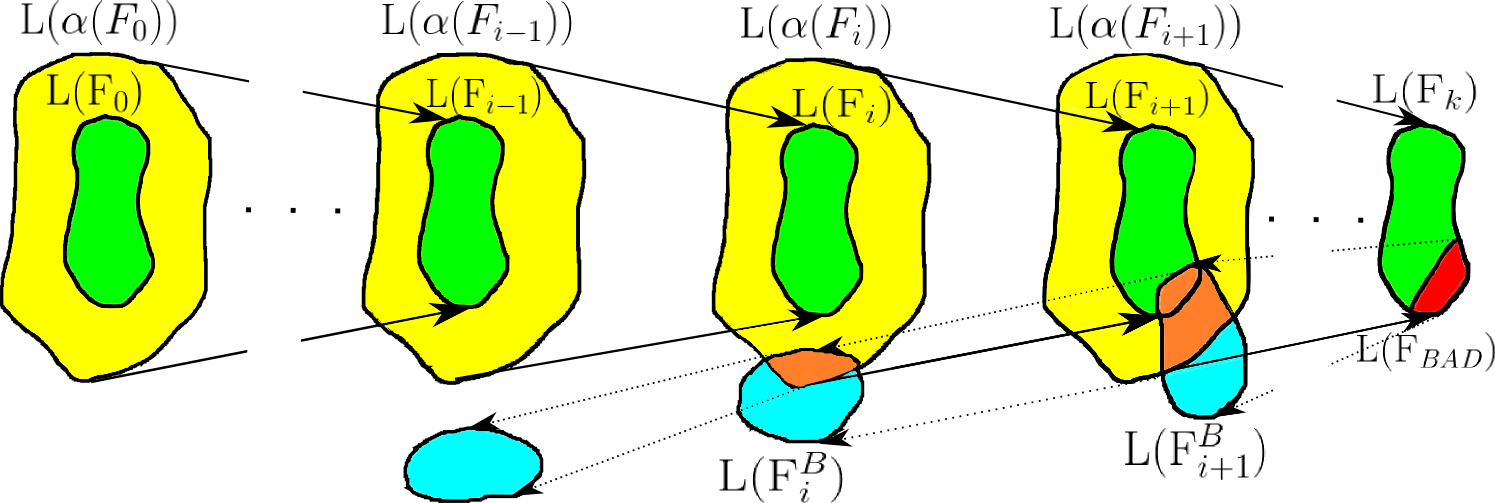
\includegraphics[width=\textwidth]{figs/artmc.png}
%	\caption{
%		Illustration (borrowed from \cite{artmc}) of the principles of the forward and the backward run and
%		the detection of a spurious counterexample.
%		}
%	\label{fig:bwrun}
%\end{figure}
%
Assume that the forward run $\fwrun = \sconf_0\sop_1\sconf_1\cdots\sop_n\sconf_n$ is spurious. 
Then there must be an index $i>0$ 
such that the symbolic path $\suffix \fwrun {i}$ is feasible 
but $\suffix \fwrun {i-1}$ is not.
This means that the operation $\sop_i$  over-approximated the semantics of $\omega$ and 
introduced into $\semof{\sconf_{i}}$ some heaps that are not in $\sopexiof{\semof{\sconf_{i-1}}}$ 
and that are \emph{bad} in the sense that they make $\suffix \fwrun {i}$ feasible.
%at the $i$th step. 
%
An \emph{interpolant for $\fwrun$}
%\td{OL: for sth? for the run $\fwrun$?} \tomas{Shouldn't it mention position $i$
%too? Usually, interpolants can be defined for any position of a spurious path. But for us, it is
%related to that unique one only, right? Perhaps to be mentioned so that people do not complain that we do not
%know what an interpolant is. In general, we should stress that our notion is
%special.}
is then a forest automaton $\interp_i$ representing
%\td{OL: language?} 
the bad heaps
of $\semof{\sconf_i}$ that were introduced into $\semof{\sconf_{i}}$ by the
over-approximation in $\sop_i$ and are
disjoint from $\sopexiof{\semof{\sconf_{i-1}}}$.
% and does represent any configurations from $\sop_i$%
%\td{OL: I don't get it}
Formally,
%
\begin{enumerate}
\item ad % $\semof{\interp_i} \cap \sopexiof{\semof{\sconf_{i-1}}} = \emptyset$ and 
\item as % $\fwrun_i$ is infeasible from all $\conf\in\semof{\sconf_i} \setminus \semof{\interp_i}$.
\end{enumerate}
%
%\td{OL: I still don't get why we're talking about the complement}
%
%\tomas{Not sure either. Couldn't we say that (1) $\semof{\interp_i} \supseteq
%\semof{\sop_i}{\semof{\sconf_{i-1}}}$ and (2) $\fwrun_i$ is infeasible from all
%$\conf\in \semof{\interp_i}$? That would be closer to the classical case, I
%think. But we get the other from the backward computation, right? So, then just
%again explain explicitly that it is so and that it is for pragmatic reasons.}

In the following, we describe how to use backward run, which reverts operations
of the forward run on the semantic level, to check spuriousness of an abstract
counterexample.
Moreover, we show how to derive interpolants from backward runs reporting
spurious counterexamples, and how to use those interpolants to refine the
operation of abstraction so that it will not introduce the bad configurations
in the same way again.
% In the following, we describe how to compute the interpolant using a backward run that reverts the operations on the semantic level, and how to use the interpolant to refine the operation of abstraction so that it will not introduce the bad configurations in the same way again.
%
%
A~\emph{backward run} for $\fwrun$ 
is the sequence 
$\bwrun = \bwsconf_0 \cdots \bwsconf_n$
such that
%
\begin{enumerate}
\item
$\bwsconf_n = \sconf_n$ 
and
\item
$\semof{\bwsconf_{i-1}} = \sopexiinvof{\semof{\bwsconf_{i}}} \cap \semof{\sconf_{i-1}}$, 
that is, ${\bwsconf_{i-1}}$ represents the \emph{weakest precondition} of
$\semof{\bwsconf_{i}}$ w.r.t.~$\sopexi$ that is \emph{localized} to
$\semof{\sconf_{i-1}}$.
\end{enumerate}
%
If there is an $\bwsconf_i$ such that $\semof{\bwsconf_i} = \emptyset$ (and,
consequently, $\semof{\bwsconf_0} = \emptyset, \ldots, \semof{\bwsconf_{i-1}} =
\emptyset$), the forward run is spurious.
In such a~case,
an interpolant $\interp_i$ for $\fwrun$ can be obtained as $\bwsconf_{i+1}$ where $i+1$ is
the smallest index such that $\semof{\bwsconf_{i+1}}\neq~\emptyset$. 
%
We elaborate on the implementation of the backward run in Sec.~\ref{sec:bwd_run}.

We note that our use of interpolants differs from that of McMillan
\cite{mcmillanCAV03} in two aspects. First, due to the nature of our backward
run, we compute an interpolant over-approximating the source of the suffix of a
spurious run, not the effect of its prefix. Second, for simplicity of
implementation in our prototype, we do not compute a~sequence of localized
%implementation in our prototype tool, we do not compute a~sequence of localized
interpolants but use solely the interpolant obtained from the beginning of the
longest feasible suffix of the counterexample for a global refinement. 
%We note,
%however, that it would also be possible to use the sequence
%$\bwsconf_i,\ldots,\bwsconf_n$ as localized interpolants.
It would also, however, be possible to use the sequence
$\bwsconf_i,\ldots,\bwsconf_n$ as localized interpolants.


In Sec.~\ref{sec:abstraction}, we show that
using the interpolant $\interp_{i}$, 
it is possible to refine regular abstraction $\sop_i$ (the only over-approximating operation)
%into $\sop_i'$ 
to exclude the spurious run.
%\tomas{Say that it guarantees progress of the analysis which is a notion
%commonly used in the related work.}
The \emph{progress guarantees} for the next iterations of the CEGAR loop are then the 
following:
%
\begin{enumerate}
\item
for any FA $\fa$ such that  
%$\sconf$ is forest compatible with $\sconf_{i-1}$
$\semof{\sconf}\subseteq\semof{\sconf_{i-1}}$ 
that is compatible with $\sconf_{i-1}$ (as defined in Sec.~\ref{sec:intersection})
it holds that
$\semof{\sop_i(\sconf)} \cap \semof{\interp_i} = \emptyset$,
%
%\tomas{I'm not getting this at all. What is $F$? The phrase ``in certain sense''
%sounds strange.}
\item
forward runs $\fwrun' = \sconf_0'\sop_1\sconf_1'\cdots\sop_n\sconf_n'$ such
that for all $1\leq j \leq n$, $\semof{\sconf_i'}\subseteq\semof{\sconf_i}$
and $\sconf_i'$ is compatible with $\sconf_i$ are excluded from the
ART.
\end{enumerate}
%
The compatibility intuitively means that boxes are folding the same sub-heaps of represented heaps and that the TA components are partitioning them in the same way.
%

%Based on this, we can then give the following progress guarantee for the CEGAR loop.
%Let  $\fwrun$ languages entail $\fwrun' = \sconf_0'\sop_1'\cdots\sop_n'\sconf_n'$ if 
%$\langof{\sconf_i'}\subseteq\langof{\sconf_i}$ for all $0\leq i \leq n$. 
%\begin{equation}
%\text{There can be at most $n-i$ futher forward runs language-entailed by $\fwrun$.}
%\text{No further run language-entailed by $\fwrun$ can be bad until $i$.}
%\end{equation}
%\bigskip
%
%
%
%\lukas{Add some discussion about guarantees on the semantic level: If folding folds the same subgraphs into the same boxes, then we have also high-level semantic guarantees analogous to the above low-level ones.}
%
%\lukas{how to call better the high-level/low-level/language semantics? Better names?}
%
%\lukas{good names for notions: abstract commands/abstract transformers/symbolic commands/symbolic transformers, operations/symbolic operations/... ?}

%\td{OL: talk about CEGAR here}

%!!!!!!!!!!!!!!!!!!!!!!!!!!!!!!!!!!!!!!!!!
%!!!!!!!!!!!!!!!!!!!!!!!!!!!!!!!!!!!!!!!!!

%*******************************************************************************
\section{Intersection of Forest Automata}\label{sec:intersection}
%*******************************************************************************

%
%It is box compatible with a folding sequence of $\heap'$ in $\fa'$  
%%$\folding' = 
%$\heap_0'\unfold_{(u_1,B_1',v_1)}\cdots\unfold_{(u_n,B_n',v_n)}\heap_n'$
%iff for every $1\leq i\leq n$,
%$\heap_i$ and $\heap_i'$ differ only in boxes on their edges.
%%
%The two sequences are forest compatible if also the following additional condition holds. 
%Let for all $1\leq i \leq n$, 
%$g_i$ be the graph which replaces the box when creating $h_{i+1}$ from $\heap_{i}$,
%and let $g_i'$ be the replaces the box when creating $h_{i+1}'$ from $\heap_{i}'$.
%%
%Then it must hold that
%$\heap_0 = \graphof \forest$ 
%and $\heap_0'=\graphof\forest'$ 
%where $\forest$ is accepted by $\fa$ and $\forest'$ by $\fa'$ and the two forests differ only in boxes on transitions,
%and the analogous relationship must hold 
%between $g_i$, $g_i'$, $\botox_i$, and $\botox_i'$ for every $1\leq i\leq n$.
%
%Two forest automata $\fa$ and $\fa'$ are box compatible/forest compatible iff 
%for every heap $\heap$ from $\semof{\fa}\cap\semof{\fa'}$,
%there is a pair of box compatible/forest compatible folding sequences of $\heap$, 
%one in $\fa$ and on in $\fa'$. 

% %-------------------------------------------------------------------------------
% \vspace{-0.0mm}
% % \subsection{The Algorithm for Computing Intersection of Forest Automata}
% \label{sec:isect_alg}
% \vspace{-0.0mm}
% %-------------------------------------------------------------------------------

The previous section used intersection of semantics of forest automata to
detect spuriousness of a~counterexample.
In this section, we give an algorithm that computes an under-approximation of
the intersection of semantics of a~pair of FAs, and later give conditions
(which are, in fact, met by the pairs of FAs in our backward run analysis) on
the intersected FAs to guarantee that the computed intersection is precise.

A simple way to compute 
%
% TV: What is ``semantic'' intersection???
%
% semantic 
%
the intersection of semantics of two FAs, denoted as $\cap$, is com\-po\-nent-wise, 
that is, for two FAs $\fa = \tuple{\tas,\asgn}$ and $\fa' = \tuple{\tasprime,\asgn}$,
we compute the FA $\fa\cap\fa' =
\tuple{(\ta_1\cap\ta_1')\cdots(\ta_n\cap\ta_n'), \asgn}$---note that the assignments need to be equal.
%
The tree automata product construction for our special kind of tree automata
synchronizes on data values and on references.
That is, a pair $(a,b)$ that would be computed by a~classical product
construction where $a$ or $b$ is a reference or a data value is replaced by~$a$
if $a = b$, and removed otherwise.

The above algorithm is, however, incomplete, i.e., it only guarantees $\semof{\fa\cap\fa'}\subseteq\semof\fa\cap~\semof{\fa'}$.
%
To increase the precision, we take into account the semantics of the boxes in
the product construction, yielding a construction denoted using~$\isectfa$.
When synchronising two rules in the TA product, we recursively call intersection of forest automata.
%
That is, we compute the FA $\fa\isectfa\fa'$ in a~similar way as $\cap$, but replace the tree
automata product $\ta\cap\ta'$ by its variant $\ta\isectta\ta'$.
For $\ta = (Q, q_0, \Delta)$ and $\ta' = (Q',q_0', \Delta')$, it computes the  TA
$\ta\isectta\ta' = (Q \times Q', (q_0, q_0'), \Delta\isectta\Delta')$ where
$\Delta\isectta\Delta'$ is built as follows:

%!!!!!!!! For LaTeX to be happy !!!!!!!!!!!
\eject
%!!!!!!!!!!!!!!!!!!!!!!!!!!!!!!!!!!!!!!!!!!

% \vspace*{-0.5mm}
    %
    \begin{align*}
    \Delta\isectta\Delta' = \big\{ & \transover{(q, q')}{\edgesymb\isectta\edgesymb'}{(q_1, q'_1), \ldots,
      (q_m, q'_m)} \mid \transover{q}{\edgesymb}{q_1, \ldots, q_m}
      \in \Delta,\\
      &
      \transover{q'}{\edgesymb'}{q'_1, \ldots, q'_m} \in \Delta'
      \big\}.\vspace*{-1mm}
    \end{align*}
    %
    %The vector $\edgesymb \isectta \edgesymb'$ is defined in the following way.
    Suppose $\edgesymb = a_1 \cdots a_m$, $\edgesymb' = a_1' \cdots
    a_m'$, and that there is an index $0 \leq i \leq m$ such that if $
    j \leq i$, $a_j$ and $a_j'$ are not boxes, and if $i < j
    $, $a_j$ and $a_j'$ are boxes.
    The vector of symbols $\edgesymb \isectta \edgesymb'$ is created as
    $(a_1\isectta a_1') \cdots (a_m\isectta a_m')$ if $a_i\isectta a_i'$ is
    defined for all $i$'s, otherwise the transition is not created.
    The symbol $a_i\isectta a_i'$ is defined as follows:
    %
    \begin{enumerate}
      \item  for $j \leq i$, $a_j\isectta a_j'$ is defined as $a_j$ if $a_j = a_j'$ and is undefined otherwise,
      \item  for $j > i$, $a_j\isectta a_j'$ is the intersection of FAs (both
        $a_j$ and $a_j'$ are boxes, i.e., FAs).
    \end{enumerate}


%%% \td{OL: some intro why this is needed?}
%%% We now provide an algorithm for computing intersection of a~pair of FAs $\fa_L$
%%% and $\fa_R$. The algorithm may in general under-approximate the semantic intersection. 
%%% After presenting the algorithm, we will define 
%%% when $\fa_L$ and $\fa_R$ compatible,
%%% which is a sufficient condition for the algorithm to be precise. 
%%% %algorithm is precise if $\fa_L$ and $\fa_R$ are box-compatible, 
%%% %which is a property that we define after exposing the algorithm.
%%% %
%%% % This section gives an algorithm for computing intersection of a~pair of FAs
%%% % $\fa_L$ and $\fa_R$ that is precise if $\fa_L$ and $\fa_R$ are box-compatible.
%%% %
%%% 
%%% Intuitively, the algorithm
%%% %
%%% % for computing intersection of a~pair of box-compatible FAs 
%%% %
%%% performs
%%% %
%%% % , in general, 
%%% %
%%% two actions.
%%% %
%%% First, it maps the cut-points of the sets of heaps represented by the FAs on each
%%% other, which induces a~mapping between the TAs representing the sub-heaps
%%% %
%%% % between
%%% %
%%% delimited by 
%%% %
%%% these cut-points.
%%% %
%%% Second, it constructs TAs representing the intersection of the pairs of TAs
%%% given by this mapping.
%%% %
%%% % This intersection is computed by 
%%% %
%%% For that, an extension of the classical intersection
%%% algorithm for TAs, constructing new states as pairs of states of the
%%% original TAs, is used. The extension checks consistency of the obtained
%%% transition function
%%% %
%%% % compatibility of the obtained product pairs \tomas{What is a product pair????}
%%% %
%%% w.r.t. our extended definition of TAs (so that, e.g., a~data value or a~root
%%% reference is not paired with a~regular state) and deals with boxes by calling the FA
%%% intersection on them recursively.
%%% 
%%% The intersection 
%%% of a~pair of (non-nested) forest automata $\fa_L = \tuple{\tasin L ,
%%% \asgn^L}$ and $\fa_R = \tuple{\tasin R, \asgn^R}$ over $\tuple{\abcd, \vars}$,
%%% written as $\fa_R \isectfa \fa_L$ 
%%% is a set of FA which contains for the FA for every permutation of $\perm = \{1,\ldots,n\}$ such that $\perm(\asgn^R(x)) = \asgn^L(x)$ for all $x\in\vars$ contains the FA 
%%% $\fa_\perm = \tuple{\ta_1^L \cap \perm(\ta_{\perm(1)}^R),\ldots,\ta_n^L \cap \perm(\ta_{\perm(n)}^R),\valuation}$,
%%% if it has a non-empty language.
%%% %
%%% The notation $\perm(\ta)$ denotes the \emph{permutation of the TA $\ta$} where every occurrence in of a root reference $\rr i$ in a leaf rule is replace by $\rr {\perm(i)}$.
%%% %
%%% The tree automata product construction for our special kind of tree automata synchronizes on data values and on references. That is, a pair $(a,b)$ that would be computed by a classical product construction where $a$ or $b$ is a reference or a data value is replaced by $a$ if $a = b$, and removed otherwise.
%%% %
%%% Note that the number of TAs of $\fa_L$ and $\fa_R$ is required to be the same,
%%% otherwise~$\emptyset$ is immediately returned.
%%% 
%%% %
%%% %\begin{enumerate}
%%% %\item 
%%% %$\perm(\asgn^R(x)) = \asgn^L(x)$ for all $x\in\vars$
%%% %\item
%%% %$\fa_\perm = \tuple{\ta_1^R \cap \perm(\ta_1^R),\ldots,\ta_n^R \cap \perm(\ta_n^R),\valuation}$
%%% %has non-empty language. 
%%% %$\ta_1^R \cap \perm(\ta_1^R)$
%%% %The 
%%% 
%%% 
%%% 
%%% %%
%%% %\begin{enumerate}
%%% %  \item  Compute the relation $\isbij ~\subseteq \{\rr 1, \ldots, \rr n\}^2$
%%% %    s.t.~$l \isbij r \iff \exists x \in \vars: \asgn^L(x) = l \land
%%% %    \asgn^R(x) = r$.
%%% %    % We assume $\top \isbij \top$.
%%% %    In case $\isbij$ 
%%% %    %
%%% %    % is not injective in both directions,
%%% %    is not a partial bijection (i.e., injective in both directions),
%%% %    %
%%% %    % restricted to its domain and co-domain is not bijective,
%%% %    %
%%% %    return~$\emptyset$.
%%% %    This step creates a mapping between cut-points referenced by variables.
%%% %
%%% %  \item  \label{step:product}
%%% %    % \comment[ar]{Asi by to chtelo zduraznit, ze $A_{(l,r)}$ budujeme pouze pro $l \isbij r$}
%%% %    In the next step, we build component TAs of the resulting FA by doing
%%% %    a~component-wise product construction.
%%% %    Consider TAs~$\ta^L_l$ and~$\ta^R_r$, for $l \isbij r$, and
%%% %    let~$\ta_{(l,r)}$ be the TA constructed from $\ta^L_l$ and $\ta^R_r$ using
%%% %    the standard procedure for TA intersection~\cite{tata}.
%%% %    We define $\reachcpof{l,r}$ to be the set of pairs $(l', r') \in \rrs^2$
%%% %    s.t.~$(l', r')$ is reachable in~$\ta_{(l,r)}$.
%%% %    We now extend $\isbij$ to $\isbij'$ such that $\isbij'$ contains~$\isbij$, and, for
%%% %    any $l \isbij' r$, it also holds that~$l' \isbij' r'$
%%% %    for all $(l',r') \in \reachcpof{l,r}$.
%%% %    If $\isbij'$ is not 
%%% %    %
%%% %    % a~bijection on its support,
%%% %    %
%%% %    % injective in both directions,
%%% %    a~(total) bijection
%%% %    %
%%% %    we, again, return~$\emptyset$.
%%% %    This step creates a~mapping between the cut-points of the heaps of
%%% %    $\fa_L$ and $\fa_R$ not reachable directly from $\vars$.
%%% %    % \td{OL: deal with $(\top, \top)$}
%%% %
%%% %  \item In the final step, we create the resulting FA $\fa$ for the intersection.
%%% %    We start with an arbitrary injective partial mapping $\order: \rrs^2 \partialto
%%% %    \rrs$ defined for all elements of $\isbij'$.
%%% %    The FA $\fa$ is then constructed as the FA $\tuple{\tas, \asgn}$ where
%%% %    every $\ta_{i}$ is obtained from $\ta_{(l,r)}$ (for~$\orderof{l,r} = i$)
%%% %    as follows:
%%% %    \begin{enumerate}
%%% %      \item  any pair $(l',r') \in \rrs^2$ occurring in $\ta_{(l,r)}$ is
%%% %        substituted with $\orderof{l',r'}$,
%%% %      \item  any pair $(d_l,d_r) \in \dset^2$ occurring in
%%% %        $\ta_{(l,r)}$ is substituted either with $d_l$ (for $d_l = d_r$), or
%%% %        with~$\top$ (if $d_l \neq d_r$),
%%% %      \item  any pair $(l',r') \notin (Q_l \times Q_r) \cup \dset \cup \rrs$
%%% %        is substituted with~$\top$ (compatible pairs of data values
%%% %        and references were reduced to singletons before),
%%% %      \item  any transition where $\top$ occurs is removed,
%%% %      \item  $\asgn$ is obtained as $\asgnof x =
%%% %        \orderof{\asgn^L(x),\asgn^R(x)}$ for $x \in \gvars$.
%%% %        %
%%% %        % $\asgnof x = \top$.
%%% %    \end{enumerate}
%%% %    %
%%% %    If the language of any TA of $\fa$ is empty, we return~$\emptyset$,
%%% %    otherwise we return~$\fa$.
%%% %
%%% %\end{enumerate}
%%% %
%%% The previous procedure can also be extended to pairs of nested FAs over
%%% $\tuple{\abcd \cup \boxes, \vars}$ by replacing the standard product construction $\cap$ in 
%%% $\ta_i^L \cap \perm(\ta_{\perm(i)}^R)$ by the operator $\nestedcap$ which, when synchronizes two automata rules, does not compare their symbols on identity, but calls recursively the forest automata intersection construction $\isectfa$ on boxes.
%%% Particularly, for two TA  $\ta_l = (Q_l, q^0_l, \Delta_l)$ and $\ta_r = (Q_r, q^0_r,
%%%     \Delta_r)$ over $\tuple{\abcd\cup\boxes,\vars}$, $\ta_l\nestedcap\ta_r$ is the TA
%%%      $(Q_l \times Q_r, (q^0_l, q^0_r),
%%%     \Delta_{(l,r)})$ where $\Delta$ is built as follows:
%%%     %
%%%     \begin{align*}
%%%     \Delta_{(l,r)} = \big\{ & \transover{(q^l, q^r)}{\edgesymb}{(q^l_1, q^r_1), \ldots,
%%%       (q^l_m, q^r_m)} \mid \transover{q^l}{\edgesymb_l}{q^l_1, \ldots, q^l_m}
%%%       \in \Delta_l,\\
%%%       &
%%%       \transover{q^r}{\edgesymb_r}{q^r_1, \ldots, q^r_m} \in \Delta_r,
%%%       \edgesymb \in \edgesymb_l \capbox \edgesymb_r  \big\} .
%%%     \end{align*}
%%%     %
%%%     The operation $\edgesymb_l \capbox \edgesymb_r$ is defined in the following way.
%%%     Suppose $\edgesymb_l = a^1_l \cdots a^m_l$, $\edgesymb_r = a^1_r \cdots
%%%     a^m_r$, and that there is an index $0 \leq i \leq m$ such that for every $1
%%%     \leq j \leq i$, $a^j_l$ and $a^j_r$ are not boxes, and for every $i < j
%%%     \leq m$, $a^j_l$ and $a^j_r$ are boxes.
%%%     We create $\edgesymb = a^1 \cdots a^m$ as follows:
%%% The $\edgesymb_l \capbox \edgesymb_r$ is the set of vector of symbols defined as follows:
%%%     %
%%%     \begin{enumerate}
%%%       \item  for $j \leq i$, $a^j$ is defined as $\{a^j_l\}$ if $a^j_l = a^j_r$,
%%%         and as $\emptyset$ otherwise,
%%%       \item  for $j > i$, $a^j$ is defined as $a^j_l \isectfa  a^j_r$ (both
%%%         $a^j_l$ and $a^j_r$ are boxes, i.e., FAs),
%%%       \item  in case any $a^j$ is $\emptyset$, we set $\edgesymb = \emptyset$.
%%%     \end{enumerate}


%------------------------------------------------------------------------------
%\paragraph{Component decompositions.}
\paragraph{Compatibility of forest automata.}
For a forest automaton $\fa = \tuple{\tas,\valuation}$, its version with marked components 
is the FA 
$\decof\fa = \tuple{\tas,\valuation\cup\valuation_\rootvar}$ 
where
$\valuation_\rootvar$ is the mapping $\{\rootvar_1\mapsto
1,\ldots,\rootvar_n\mapsto n\}$.
%
% $\rootvar_i$'s are fresh \emph{root variables} 
%
%\tomas{Stress even more that the root variables point explicitly to each root.
%Stress that this is meaningful when the roots need not be cut-points? I was
%quite confused here for a while---I just hope it is for the case of having
%non-cut-point roots.} \lukas{hm, maybe it is}
%
The \emph{root variables} $\rootvar_i$ are fresh variables that
point to the roots of the tree components in $\langof{\fa}$. 
%
$\semof{\decof\fa}$ then contains the same heaps as $\semof\fa$, but the
roots of the components from $\langof{\fa}$ remain visible as they are explicitly marked by the root variables.
%
In other words, the root variables track how the forest decomposition of heaps
in $\langof{\fa}$ partitions the heaps from~$\semof{\fa}$. 
%
By removing the root variables of $\decof\heap\in\semof{\decof\fa}$, we get the
original heap $\heap\in\semof\fa$. We call $\decof\heap$ the \emph{component
decomposition of $\heap$ by $\fa$}.
%The elements from $\semcompof{\fa}$ are called \emph{component decompositions}.
%
%For a~set~$S$ of component decompositions, we can come back to the standard semantics
%by removing the root variables, which is denoted by~$\semofcd{S}$.
%
%We say that two forest automata~$\fa$ and~$\fa'$ are \emph{component-compatible} iff
%$\semof{\fa}\cap\semof{\fa'} = \semofcd{\semcompof\fa\cap\semcompof{\fa'}}$.
%
%Intuitively, it means that the heaps in the semantic intersection have the same
%sub-heaps encoded by the components of the FAs at the same
%positions.

%\paragraph{Representation compatibility.}


%!!!!!!!!!!!!!!!!!!!!!!!!!!!!!!!!!!!!!!!!!
%!!!!!!!!!!!!!!!!!!!!!!!!!!!!!!!!!!!!!!!!!

Using the notion of component decomposition, we further introduce a notion of
the \emph{representation} of a~heap by an FA. Namely, the \emph{representation}
of a~box-free heap~$\heap$ by an FA $\fa$ with $\heap\in\semof\fa$ records how
$\fa$ represents $\heap$, i.e., (i) how $\fa$ decomposes $\heap$ into
components, and (ii) how its sub-graphs enclosed in boxes are represented by the
boxes. 
%
Formally, the representation of $\heap$ by $\fa$ is a pair $\repre =
(\decof\heap,\{\repre_1,\ldots,\repre_n\})$ such that $\decof\heap$ is the
component decomposition of $\heap$ by $\fa$, and $\repre_1,\ldots,\repre_n$ are
obtained from the sequence of unfoldings\
%
\vspace{-1mm}
\begin{equation*}
\heap_0\unfoldofi{1} \heap_1 \unfoldofi{2}  \cdots \unfoldofi{n} \heap_n
\vspace{-1mm}
\end{equation*}
%
with $\heap_0 = \decof\heap$ and $\heap_n\in\langof{\decof{\fa}}$, such that for
each $1\leq i\leq n$, $\repre_i$ is (recursively) the representation of $g_i$ in
$\botox_i$.

We write $\semof\repre$ to denote $\{\heap\}$, and,
%
for a set of representations~$\repres$, we let $\semof\repres =
\ourbigcup_{\repre\in\repres} \semof{\repre}$.
% \{\semof\dec\mid\dec\in\decs\}$.
%
The set of \emph{representations accepted by a forest automaton} $\fa$
is the set $\represof\fa$ of all representations of heaps from
$\semof\fa$ by $\fa$. 
%
We say that a~pair of FAs $\fa$ and $\fa'$ is \emph{(representation) compatible} iff $\semof \fa \cap
\semof {\fa'} = \semof{\represof \fa \cap \represof{\fa'}}$.
%
The compatibility of a~pair of FAs intuitively means that for every heap from the semantic intersection of the two FAs,
at least one of its representations is shared by them.
%

\begin{lemma}
  %
  % Suppose $\fa_L$ and $\fa_R$ is a~pair of box-compatible FAs. Then
  % $\semof{\fa_L \isectfa \fa_R} = \semof{\fa_L} \cap \semof{\fa_R}$.
  %
  For a pair $\fa$ and $\fa'$ of compatible FAs,
  it holds that
  $\semof{\fa \isectfa \fa'} = \semof{\fa} \cap \semof{\fa'}$.
\end{lemma}

%\begin{proof}
%Left as an exercise for the kind reader.
%(Please send the solution to the address of the authors if you manage.)
%\qed
%\end{proof}

%
% OLD SECTION
%
% \subsubsection{Intersection of compatible forest automata.}
% Forest compatibility can be used to implement computation of semantic intersection of forest automata
% by reduction to the problem of computing intersection of symbolic tree automata over effective Boolean algebra over $\Data\cup\abcd\cup\boxes$  \cite{veanes}.   
% %
% Given two forest automata $\fa= \tuple{\tas,\valuation}$ and $\fa' = \tuple{\tas',\valuation}$ 
% (with the same valuation and the same number of components) 
% it returns the forest automaton 
% $\fa\syminter\fa' = \tuple{\ta_1\syminter\ta_1,\ldots,\ta_n\syminter\ta_n,\valuation}$.
% The tree automaton $\ta_i\syminter\ta_i'$ is computed as the intersection of symbolic tree automata over the effective Boolean algebra over $\Data\cup\abcd\cup\boxes$. 
% To implement the intersection computation, it implements conjunction of boxes using $\syminter$ over forest automata.
% Notice that since the hierarchy of boxes in forest automata form a strict hierarchy, the depth of recursion is bounded and the algorithm terminates. 
%
% \begin{lemma}
% If $\fa$ and $\fa'$ are forest compatible, then 
% $\semof{\fa_1}\cap\semof{\fa_2} = \semof{\fa\syminter\fa'}$. 
% \end{lemma}
% \footnote{
% We note that intersection of box compatible automata can be also computed, by a similar algorithm,
% but the forest automata operator does normalisation of both automata and then computes the union of $\syminter$ between all pairs $\fa$, $\fa''$ where $\fa''$ arises from $\fa'$ by permutation of tree components that are not referenced by variables. This note is probably useless, right ...
% }
% \footnote{
% By the way, entialment checking of two folding equivalent forest automata can be probably done exactly by the symbolic automata algorithm that uses intersection and itself too on the symbolic labels too.
% But this is not crucial for this paper.
% }


To illustrate the reason why compatibility is necessary in the backward run (cf.\
Section~\ref{sec:CEXanalysis}), consider a forward run that reaches an error
line after passing through an FA~$F_k$ with the language consisting of a single configuration
with one edge $n_1 \xrightarrow {\mathit{DLL}}~n_2$.
% 
% and the valuation of variables $\valuation = \{x \mapsto n_1, y\mapsto y_2\}$. 
%
The box encloses a DLL segment, i.e., its output port
is the $\mathit{next}$-successor of the input port, and the input is the
$\mathit{prev}$-successor of the output port. 
%
Assume that the backward run then arrives with an FA
$o_{k+1}^{-1}({F_{k+1}})$ with the same language as $F_k$ up to 
using the edge $n_2 \xrightarrow {\mathit{revDLL}} n_1$
%
% It encodes the same configuration $c$,  just instead of $\mathit{DLL}$, 
% it uses a~box 
%
with a reversed DLL-segment, where the output is the~$\mathit{prev}$-successor of the input.
%
Despite $F_k$ and
$o_{k+1}^{-1}({F_{k+1}})$ have the same semantics,
%
% $F'_{k}$ should encode 
%
their languages are different and incompatible:
In $\langof{F_k}$, $n_1$ has a successor and $n_2$ does not, 
while it is the other way round in $\langof{o_{k+1}^{-1}({F_{k+1}})}$.
%
The intersection computed using $\sqcap$ will be empty.
%
% , hence the two configurations are entirely different to $\sqcap$.  
%
Under-approximating the intersection this way can lead to
wrong spuriousness detection and ineffective abstraction refinement.
%
Enforcing compatibility rules out such situations and guarantees that the
intersection computed using $\sqcap$ is precise.


%*******************************************************************************
\section{Implementation of the Forward Run}\label{sec:fwd_run}
%*******************************************************************************
%The main goal of this section is to describe the operations that are used to
%implement the forward symbolic execution over FAs. However, before that, we need
%to introduce one more notion that will subsequently allow us to implement the
%backward execution by inverting the operations used in the forward execution.
%%
%In particular, apart from the already introduced box compatibility, we need to
%introduce a further notion of component compatibility.
%%
%It is defined as follows.

This section describes the operations that are used to
implement the forward symbolic execution over FAs. 
%
%It is defined as follows.
%
%
% Namely, to be able to invert the operations used in a~forward run $\fwrun =
% \sconf_0\sop_1\cdots\sop_n\sconf_n$ (i.e., to compute the localized weakest
% preconditions over the run) and to compute an interpolant~$\interp_i$ of
% a~spurious run, which we need for refinement, we will require the backward run
% $\bwrun = \bwsconf_0 \cdots \bwsconf_n$ to compute $\bwsconf_j$ that is both
% box-compatible and component-compatible with $\sconf_j$ for every $i\leq j\leq
% n$.
%
% Box compatibility is important for the operation of intersection to be
% semantically precise, as discussed in Section~\ref{sec:intersection}, and also
% as a~prerequisite of component compatibility. Component compatibility is needed
% to invert the operations used in the forward run.
%
%\paragraph{Component decomposition.}
%For a forest automaton $\fa = \tuple{\tas,\valuation}$, its \emph{component
%semantics} is
%$\semcompof{\fa}=\semof{\tuple{\tas,\valuation\cup\valuation_\rootvar}}$ where
%$\valuation_\rootvar$ is the mapping $\{\rootvar_1\mapsto
%1,\ldots,\rootvar_n\mapsto n\}$.
%%
%% $\rootvar_i$'s are fresh \emph{root variables} 
%%
%%\tomas{Stress even more that the root variables point explicitly to each root.
%%Stress that this is meaningful when the roots need not be cut-points? I was
%%quite confused here for a while---I just hope it is for the case of having
%%non-cut-point roots.} \lukas{hm, maybe it is}
%%
%Here, the \emph{root variables} $\rootvar_i$ are fresh variables that are set to
%point to the roots of the tree components in $\langof{\fa}$. 
%%
%Then, $\semcompof{\fa}$ contains the same heaps as $\semof\fa$ but with the
%roots of the components from $\langof{\fa}$ explicitly marked by the root
%variables.
%%
%In other words, the root variables track how the forest decomposition of heaps
%in $\langof{\fa}$ partitions the heaps from~$\semof{\fa}$. 
%%
%The elements from $\semcompof{\fa}$ are called \emph{component decompositions}.
%%
%For a~set~$S$ of component decompositions, we can come back to the standard semantics
%by removing the root variables, which is denoted by~$\semofcd{S}$.
%%
%We say that two forest automata~$\fa$ and~$\fa'$ are \emph{component-compatible} iff
%$\semof{\fa}\cap\semof{\fa'} = \semofcd{\semcompof\fa\cap\semcompof{\fa'}}$.
%%
%Intuitively, it means that the heaps in the semantic intersection have the same
%sub-heaps encoded by the components of the FAs at the same
%positions.
%
To be able to implement the backward run, we will need to maintain
compatibility between the forward run and the so-far constructed part
of the backward run.
%
Therefore, we will present the operations used in the forward run mainly from
the point of view of their effect on the representation  of heaps (in the sense
of Sec.~\ref{sec:intersection}).
%
Then, in Sec.~\ref{sec:bwd_run}, we will show how this effect is inverted in
the backward run such that, when starting from compatible
configurations, the inverted operations preserve compatibility of the
configurations in the backward run with their forward run counterparts.

% we get to compatible configurations again, and
% hence compatibility is preserved in the backward run.


%Now, we are finally ready to describe the operations used in the forward run.
%We are now ready to describe the operations used in the forward run.
%
We omit most details of the way the operations are implemented on the level of manipulations with rules and states of FAs. 
%We mostly omit their detailed implementation on the level of manipulations with
%rules and states of FAs. 
%since it is not important for this paper; instead,
%we refer the reader to~\cite{forester12,jiri:diza} for details.
We refer the reader to~\cite{forester12,jiri:diza} for the details.
%
We note that when we talk about removing a~component or inserting a component
in an FA, this also includes renaming references and updating
assignments of variables.
%
When a component is inserted at position~$i$, all references to~$\rr j$ with
$j>i$ are replaced by~$\rr{i+1}$, including the assignment~$\asgn$ of variables.
%
When a~component is removed from position~$i$, all references to $\rr j$ with $j > i$ are
replaced by references to~$\rr{j-1}$. 


% To revert the operations, we will sometimes need to remember some operation
% from the forward run in the backward run.
% We make that information visible in a~form of a~parameter $\mathit{par}$ of the
% operation, which will be in the form $\sop[\mathit{par}]$.

%which are generalization that consists of regular abstraction, normalization, and folding, 
%and operations that implement program statements.

%
%To explain the computation of localized preconditions while preserving the forest compatibility invariant,
%we will present the operations divided into smaller instructions,
%which affect forest compatibility.
%
%In the previous section we describe it on level of forest automata languages.
%To enable predicate learning described in the previous section we need to perform
%a backward run on level of compatible forest decomposition represented by automata
%from the forward and backward run.
%Therefore we provide with more detailed description of what happens in forward run
%with FA. The we will describe how we revert the operations from forward run in backward run.

%------------------------------------------------------------------------------
\paragraph{Splitting.}
Splitting has already been discussed in Sec.~\ref{sec:analysis}.
It splits the symbolic execution into several branches such that the union of
the FAs after the split is semantically equal to the original~FA.
%
The split is usually performed when transforming an~FA into several FAs that
have only one variant of a~root rule of some of their components.
%
From the point of view of a~single branch of the ART,
splitting is an operation, denoted further as $\splitting$, that transforms an
FA $\fa$
into an FA~$\fa'$ s.t. $\semof{\fa'}\subseteq\semof\fa$ and 
$\represof{\fa'}\subseteq\represof\fa$.
Therefore, $\fa$ is compatible with~$\fa'$.

%!!!!!!!!!!!!!!!!!!!!!!!!!!!!!!!!!
%!!!!!!!!!!!!!!!!!!!!!!!!!!!!!!!!!

%------------------------------------------------------------------------------
%\paragraph{Operations Modifying Component Semantics}
\paragraph{Operations modifying component decomposition.}
This class of operations is used to implement transformation of FAs to the dense form and as
pre-processing steps before the operations of folding, unfolding, and symbolic
implementation of program statements.
%
They do not modify the semantics of forest automata, 
but change the component decomposition of the represented heaps.
%Folding and unfolding of boxes and implementations of program commands need preprocessing of the forest automata so that their component semantics satisfies certain properties. The preprocessing is done by a set of operations that modify the component semantics, while not modifying the box semantics.
%
\begin{itemize}
%\item[\emph{Component Removal.}]
%Removing the $i$th component requires also replacing all references to $j$th components for $j>i$ by references to $j-1$th component, in the languages of the tree automata as well as in the valuation of variables.
%Removing appear in a forward run as $\removing{i}$.
%Normalization does not change forest automata semantically, 
%but affects the component decomposition of their heaps.
%

%Splitting is done when an operation such as $\code{x = y\text{\texttt{->}}sel}$ is performed.
%Since a forest automaton can represent a set of heaps this operation could cause that
%their forest decomposition differ. E.g. consider a cyclic singly linked list
%of arbitrary length where \code{y} points to a head of list.
%Then the noted operation would result to (a) at least two tree components for
%length longer than one or (b) one tree component for list of length one.
%Forest automata are not capable of representation of such different heaps.
%Therefore we create (split) more copies of automaton, one for each possible tree decomposition.
%The symbolic execution is then split to the separated branches for particular
%forest automata and each branch continues independently.
% \item[\emph{Connecting of components.} ] 
\item \emph{Connecting of components.}
%\tomas{This name sounds extremely strange to me. Perhaps Connecting a Component?}
When the $j$-th component $\ta_j$ of a forest automaton $\fa$ accepts trees with false roots, 
then $\ta_j$ can be connected to the component that refers to it. 
%
Indeed, as such roots are not cut-points, 
a~reference $\rr j$ to them can appear only in a~single component, say $\ta_k$, 
and at most once in every tree from its language (because a~false root
can have at most one incoming edge). 
%
For simplicity, assume that $\ta_j$ has only one root state $q$ that does
not appear on the right-hand sides of rules. 
%
The connection is done by adding the states and rules of~$\ta_j$ to $\ta_k$, replacing the reference~$\rr j$ in the rules of $\ta_k$ by~$q$.
%From the language point of view, the trees of $\ta_j$ are thus 
%reference $\bar j$ 
%connected to roots of the trees of $\ta_i$.  
%
The $j$-th component is then removed from~$\fa$.
%
The previous sequence of actions is denoted as the operation $\connecting{j,k,q}$ below. 
%
%
%It is done by replacing the reference $\bar i$ at the right-hand side of a leaf rule by the root state $q$ of $\ta_i$.  
%The $i$th component is removed by $\removing{i}$.
%The connection then appears in the forward run
%as the operation $\connecting{q,i}$. 
%\lukas{state maybe not needed to remember}
% \item [\emph{Cutting of a component.}] 
\item \emph{Cutting of a component.}
Cutting divides a~component  with an index~$j$ into two. 
The part of the $j$-th component containing the root will accept tree prefixes
of the original trees, and the~new $k$-th component will accept their remaining
sub-trees.
%of them is accepting subtrees of the trees accepting by the original one, and the other one is accepting tree prefixes that have a reference to the sub-tree component at the place where the sub-tree was connected.  
The cutting is done at a state $q$ of $\ta_j$, which appears exactly once in
each run (the FA is first transformed to satisfy this). 
Occurrences of~$q$ at the right-hand sides of rules are replaced by the reference
$\rr k$ to the new component, and $q$ becomes the root state of the new
component. 
We denote this operation by $\cutting{j,k,q}$.
%The information about $q$ and $i$ together with the assumption about $q$ will allow us to revert it in the backward run. 
% \item [\emph{Swapping of components.}]
\item \emph{Swapping of components.}
  The operation $\swapping{j,k}$ swaps the
  $j$-th and the $k$-th component (and renames references and assignments
  accordingly). 
\end{itemize}

%%%%   \subsection{Normalization}
%%%%   Calling normalisation is important because (1) 
%%%%   it facilitates the entailment checking \cite{cav} used to detect the fixpoint of the symbolic execution, 
%%%%   (2) it merges tree automata components, keeping their number small, which is important for efficiency reasons, and 
%%%%   (3) it empowers regular abstraction, which has more opportunities to overapproximate if the heaps are decomposed to a small number of large components.   
%%%%   %On forest automata representations with less tree components, because it is applied to tree components in isolation, and having larger pieces of configurations within a single component gives it more opportunities to overapproximate.
%%%%   %
%%%%   A detailed description of normalization can be found in \cite{cav,jiri,martin}. 
%%%%   It can be implemented as a sequence of operations of three kinds:
%%%%   \begin{itemize}
%%%%   \item [\emph{Splitting.}] As discussed in Section~\ref{}, it splits the symbolic execution into several branches. 
%%%%   From a point of view of single branch/forward run, 
%%%%   it appears as an operation $\splitting$ which transforms a forest automaton $\fa$ into $\fa'$ such that, $\semof\fa'\subseteq\semof\fa$, 
%%%%   and which is box and component compatible with $\fa$ because splitting does not influence the decomposition and component semantics.
%%%%   %Normalization does not change forest automata semantically, 
%%%%   %but affects the component decomposition of their heaps.
%%%%   %
%%%%   
%%%%   %Splitting is done when an operation such as $\code{x = y\text{\texttt{->}}sel}$ is performed.
%%%%   %Since a forest automaton can represent a set of heaps this operation could cause that
%%%%   %their forest decomposition differ. E.g. consider a cyclic singly linked list
%%%%   %of arbitrary length where \code{y} points to a head of list.
%%%%   %Then the noted operation would result to (a) at least two tree components for
%%%%   %length longer than one or (b) one tree component for list of length one.
%%%%   %Forest automata are not capable of representation of such different heaps.
%%%%   %Therefore we create (split) more copies of automaton, one for each possible tree decomposition.
%%%%   %The symbolic execution is then split to the separated branches for particular
%%%%   %forest automata and each branch continues independently.
%%%%   \item[\emph{Connecting.}] 
%%%%   When the root of an $i$th component $\ta_i$ of a forest automaton $\fa$ does not semantically correspond to a cut-point, 
%%%%   then the component is merged with other components. 
%%%%   From the language point of view, 
%%%%   the trees from $\langof{\ta_i}$ are connected as sub-trees to trees accepted by the other components at their leaves with a reference to $i$th component. 
%%%%   %
%%%%   It is done by replacing the reference $\bar i$ at the right-hand side of a leaf rule by the root state $q$ of $\ta_i$.  
%%%%   The connection then appears in the forward run
%%%%   as the operation $\connecting{q,i}$. 
%%%%   \lukas{state maybe not needed to remember}
%%%%   %The information about $q$ and $i$ together with the assumption about $q$ will allow us to revert it in the backward run. 
%%%%   \item [\emph{Swapping.}] 
%%%%   Tree automata components are swapped to achieve canonic ordering. 
%%%%   The operation appears as $\swapping{i,j}$, 
%%%%   where $i,j$ are indices of the swapped components. 
%%%%   \end{itemize}

%------------------------------------------------------------------------------
\paragraph{Folding of boxes.}
The folding operation assumes that the concerned FA is first transformed into the form
$\fa = \tuple{\boxtas \ta_1' \cdots \ta_m',\asgn}$ by a sequence of splitting,
cutting, and swapping.
%
% where all trees of $\langof{\ta_\iport}$ and $\langof{\ta_\oport}$ are of depth~$1$. 
%
The tuple of TAs $\boxtas$ will then be folded into a new box $\botox$
with~$\ta_\iport$ as its input component and~$\ta_\oport$ as its output.
Moreover, the operation is given sets of selectors~$S_{\iport},
S_{\oport}$ of roots of components in~$\ta_\iport$ and~$\ta_\oport$ that are to
be folded into~$\botox$.
%
The box~$\botox =
\tuple{\boxtasin,\{\iport\mapsto 1,\oport\mapsto n\}}$
 arises from~$\fa$ by taking $\boxtas$
%
and by removing selectors that are not in $S_{\iport}$ and $S_{\oport}$
from root rules of $\ta_\iport$ and~$\ta_\oport$ to obtain $\ta_\iport^\botox$ and
$\ta_\oport^\botox$ respectively.
%, which results into $\ta_1'$ and $\ta_n$'. 
% Particularly, the roots of $\ta_\iport$ and $\ta_\oport$ are stripped from all
% successors but those 
% reached by selectors from sets $S_\iport$ and $S_\oport$ of selectors, respectively. 
%
%Intuitively, the box $\botox$ will enclose only selectors leading from its
%input and output ports that are from the two sets, the rest will be left outside
%the box.
%

Folding returns the forest automaton $\fa' = \tuple{\ta'_{\iport}
\ta'_{\oport} \ta'_1 \cdots \ta'_m, \asgn'}$ that arises from $\fa$ as follows.
All successors of the roots accepted in $\ta_\iport$ and $\ta_\oport$
reachable over selectors from $S_\iport$ and $S_\oport$
are removed in $\ta'_\iport$ and $\ta'_\oport$ respectively (since they are enclosed in~$\botox$).
The root of the trees of $\ta'_\iport$ gets an additional edge labelled by
$\botox$, leading to the reference $\rr n$ (the output port),
and the components $\ta_2 \cdots \ta_{n-1}$ are removed (since they are also enclosed in~$\botox$).
%
This operation is denoted as $\folding{n,S_{\iport},S_{\oport},\botox}$.
%
% $\fa' = \folding{n,S_{\iport},S_{\oport},\botox}(\fa)$ such that 
%$\semof{\fa'} = \semof{\fa}$
%For every $\heap'\in\langof{\fa'}$, 
%there is $\heap\in\langof\fa$ 
%such that $\heap'\unfoldof{(u,\botox,v)}{blah}\heap$,
%$u$ is the $i$-th root in the forest decomposition of $\heap$ accepted by $\fa$
%and also the $j$-th root in the forest decomposition of $\heap'$ accepted by $\fa'$.
%Algorithms for learning boxes and folding are described in \cite{}.
%%%

%------------------------------------------------------------------------------
\paragraph{Unfolding of boxes.} 
Unfolding is called as a preprocessing step before operations that implement
program statements
in order to expose the selectors accessed by the statement. 
It is called after a sequence of cutting, splitting, and swapping
that changes the forest automaton into the form 
$\fa' = \tuple{\ta_\iport'\ta_\oport'\ta_1'\cdots\ta_m',\asgn'}$ where
%
% all trees of $\langof{\ta_\iport'}$ and $\langof{\ta_\oport'}$, are of
% depth~$1$, and
%
trees of $\ta'_\iport$ have a~reference $\overline 2$ to $\ta_\oport'$ accessible by an 
edge going from the root and labelled by the box~$\botox$ that is to be unfolded.
%
Furthermore, assume that the box $\botox$ is of the form
$\tuple{\boxtasin,\{\iport\mapsto 1,\oport\mapsto n\}}$
%
and 
%
the input and the output ports have outgoing selectors from the sets 
$S_\iport$ and $S_\oport$ respectively. 
%
The operation returns the forest automaton 
$\fa$ that arises from~$\fa'$ by 
%$\tuple{\ta_\iport'',\tas,\ta_\oport'',\{\iport\mapsto 1,\oport\mapsto n+1\}}$
%
inserting components $\boxtasin$ in between $\ta'_\iport$ and $\ta'_\oport$, 
removing the $\botox$ successor of the root in~$\ta_\iport'$,
merging $\ta_\iport^\botox$ with $\ta_\iport'$, and $\ta_\oport^\botox$
with $\ta_\oport'$.
% The merging on the language level consists of merging roots of the trees.
The merging on the TA level consists of merging root transitions of the TAs.
%
We denote this operation as $\unfolding{n,S_{\iport},S_{\oport},\botox}$.

%It is an operation $\unfolding{i,j,\botox}$ which for a given $\fa$ 
%returns a forest automaton $\fa' = \unfolding{i,j,\botox}(\fa)$ such that 
%$\semof{\fa'} = \semof{\fa}$. 
%For every $\heap'\in\langof{\fa'}$,
%there is $\heap\in\langof\fa$ such that $\heap\unfoldof{(u,\botox,v)}{blah}\heap'$,
%$u$ is the $i$-th root in the forest decomposition of $\heap$ accepted by $\fa$
%and also the $j$-th root in the forest decomposition of $\heap'$ accepted by $\fa'$.
%See \cite{jiri,cav} for details on unfolding.
%
%Before the unfolding is called, 
%the box to be unfolded must appear on an edge leading from the root of some of its tree components. 
%This is done by a sequence of splitting? and cutting. 

%Algorithms for learning boxes and folding are described in \cite{}.
%They can be implemented on the level of operations as follows. 
%By a sequence of splitting, cutting, and swapping, 
%the forest $\fa$ is first transformed into a form
%$\tuple{\tas,\ta_1',\ldots,\ta_m',\valuation}$ where $\ta'_1$ and $\ta_m'$ have only one root rule. 
%%
%The box $\botox$ to be folded is then made from
%$\tuple{\ta_1',\ldots,\ta_m',\{\iport\mapsto 1,\oport\mapsto m\}}$. 
%Particularly, the root rule $\vec a(\vec q)$ of $\ta_1'$ is modified
%by removing certain positions $P_1$ from the vectors $\bar a$ and $\bar q$, 
%and similarly for some positions $P_m$ of the root rule of the automaton $\ta_m$. 
%(the box will hide certain selectors on the positions from $P_1$ of its input node, and certain selectors at $P_m$ of its output node).
%%
%The operation returns the forest automaton 
%$\tuple{\tas,\ta_1',\ldots,\ta_m',\valuation}$ by
%removing removing all positions but those from $P_1$ from the root rule of $\ta_1'$ and then appending symbol $B$ to the vector of symbols 
%and a reference to the vector of states $\ta_m'$.
%Removing removing all positions but those from $P_m$ from the root rule of $\ta_m'$,
%and removing components $\ta_2'$ to $\ta_{m-1}'$.
%%
%This operation appears in forward run as $\folding{n,P_1,P_m,\botox}$.
%
%The swapping and splitting was described within normalisation. 
%Cutting splits a tree automata component into two, one of them is accepting subtrees of the trees accepting by the original one, and the other one is accepting tree prefixes that have a reference to the sub-tree component at the place where the sub-tree was connected.  
%Cutting then appears as the symbolic operation $\cutting{i,j}$ where $i$ is the index of the prefix component and $j$ is the index of the sub-tree component. 

%requires the input of the folded graph be a root in the forest decomposition of the forest automaton.
%To achieve this,
%it must be sometimes  preceded by the operation of \emph{cutting}.
%It is an operation $\cutting{i}$ which cuts the $i$th tree component into two halves, from which the root half stays at the $i$th position and the bottom half is appended at the end of the list of the components.


%!!!!!!!!!!!!!!!!!!!!!!!!!!!!!!!!!!!!!!!!
%!!!!!!!!!!!!!!!!!!!!!!!!!!!!!!!!!!!!!!!!

%------------------------------------------------------------------------------
\paragraph{Symbolic execution of program statements.}
We will now discuss our symbolic implementation of the most essential statements
of a C-like programming language. 
%They are 
%$\code{x = malloc()}$, 
%$\code{x = y\text{\texttt{->}}sel}$,
%$\code{y\text{\texttt{->}}sel = x}$,
%$\code{y \datarel x}$,
%$\code{x = y}$ or $\code{x = NULL}$, and
%$\code{free(y)}$.
%%
%Symbolic implementations of the statements use four operations. 
%%
%We use $\xroot$ and $\yroot$ to denote
%		the root states of $\xta$ and $\yta$, respectively. 	    
%
%
%The commands always access only selectors of nodes pointed to by variables.
%These are either exposed in root rules of the tree automata of the variable, in which case folding is not needed, or folded within a box. It is either a box in the root rule of $\valuation(x)$ or it may be a box
%within leaf rule which ends by a reference to the $\valuation(x)$. 
%In the latter case, 
%the occurrence of the box is first isolated into a separate tree component which contains the only the rule with the box. 
%
%It is unfolding, 
%which is to extract selectors of memory cells accessed by the statement from boxes, 
%then splitting, which is is necessary to keep the forest automata well define (??) 
%due to forest automata not being closed under union,
%and cutting.
%After preprocessing by unfolding and splitting and cutting, which have no semantic effect,
%the transformation changing the semantics is finally applied.
%We discuss the three in a more detail.
%
%
%Therefore we create (split) more copies of automaton, one for each possible tree decomposition.
%The symbolic execution is then split to the separated branches for particular
%forest automata and each branch continues independently.
%
%\paragraph{Abstract statement}
%
We assume that the operations are applied on an FA~$\fa = \tuple{\tas,\valuation}$.
		\begin{itemize}
		   \item $\code{x := malloc()}$: A new $(n+1)$-th component 
		  $\ta_{\mathit{new}}$ is appended to $\fa$ s.t. it contains one state and one transition with all
		  selector values set to $\asgnof \unef$.
      The assignment~$\asgnof{\code{x}}$ is set to $\rr{n+1}$. 
		  %The operation basically adds one node $v$ to heaps from
		  %language of $\fa$ and sets $\asgnheapof{\code{x}}$ to $v$ for each heap $h$.

		  \item $\code{x := y\text{\texttt{->}}sel}$ and $\code{y\text{\texttt{->}}sel := x}$:
		% If $\valuationof{\code y} = \valuationof\unef$, then $\code{x = y\text{\texttt{->}}sel}$ moves to the error location.
		If $\valuationof{\code y} = \valuationof\unef$, the operation moves to the error location.
        Otherwise, by splitting, cutting, and unfolding, $\fa$ is transformed into the
        form where $\ta_{\asgnof{\code{y}}}$ has only one root rule and the rule
        has a $\code{sel}$-successor that is a~root reference $\rr j$. 
        The statement
$\code{x := y\text{\texttt{->}}sel}$ then changes $\valuationof{\code{x}}$ to $\rr j$, and
$\code{y\text{\texttt{->}}sel := x}$ changes the reference $\rr j$ in $\ta_{\asgnof{\code y}}$ to $\valuationof{\code x}$.

%$ \cval$We then only 
%          If $q_i$ is a root reference (say,
%		  $j$), it is sufficient to change the value of $\valuation(\code{x})$ to $j$.
%		  Otherwise, we split $\yta$ at the $i$-th position (creating $\ta_k$) and assign $k$ %to
%		  $\valuation(\code{x})$. This operation does not change language of a forest automaton
%		  but it can change forest decompositions of heaps. This is caused by possibility of
%		  creating a new cutpoint by redirection of variable $\code{x}$.

%		  \item[$\code{y\text{\texttt{->}}sel = x}$] 
%If $q_i$ is a state, then we split
%		  $\yta$ at the $i$-th position. Then we put a reference to ${\valuation(\code{x})}$ to the
%		  $i$-th position in the right-hand side of the root transition of $\yta$; this
%		  is done both if $q_i$ is a state and if $q_i$ is a root reference. The operation
%		  changes heaps from language of FA by redirecting the edges corresponding to
%		  the $\code{sel}$ selector.

      \item $\code{assume(x \datarel y)}$ where $\datarel\ \in \{\code{==},
        \code{{!}{=}}\}$:
        This statement tests the equality of $\valuation(\code{x})$ and $\valuation(\code{y})$
        and stops the current branch of the forward run if the result does not match $\datarel$.
      \item $\code{assume(x\text{\texttt{->}}data \datarel y\text{\texttt{->}}data)}$
        where $\datarel$ is some data comparison:
        We start by unfolding and splitting $\fa$ into the form where
        $\ta_{\valuation(\code{x})}$ and $\ta_{\valuation(\code{y})}$ have only
        one root rule with exposed $\code{data}$ selector.
        The data values at the $\code{data}$ selectors are then compared and
        the current branch of the forward run is stopped if they do not satisfy~$\datarel$.
        The operation moves to the error locations if $\asgnof{\code x}$ or
        $\asgnof{\code x}$ are equal to~$\asgnof \unef$.
% \lukas{in the initial conf, everybody is defined and has the same value as undef, except null}
%with $\datarel$ and the forward run is stopped if the test returns false.  

%The is implemented by splitting the $\fa$ into all variants such that in each of them, both $\ta_\valuation{\code{x}}$ and  
%$\ta_\valuation{\code{y}}$ have a unique root rule and then removing the variants where the 
%		  Assume that both states are data ones.
%		  If $data_y \datarel data_x$ holds (or does not hold), we return \emph{true} (or \emph{false}).
%		  Otherwise, we copy $\tuple{\valuation, \fa}$ into two abstract configurations:
%		  $\tuple{\valuation, \fa_{\mathit{true}}}$ for the $\emph{true}$ branch and
%		  $\tuple{\valuation, \fa_{\mathit{false}}}$ for the $\emph{false}$ branch
%		  and continue from each branch separately. Operation does not change language of FA
%		  neither accepted forest decomposition.

		  \item $\code{free(x)}$: The component $\ta_{\asgnof{\code{x}}}$ is removed, 
          and all references to $\asgnof{\code{x}}$ are replaced by~$\asgnof \unef$.
%First, we split $\yta$ at all $j$-th positions, $1 \leq j
%		  \leq m$, that appear in its root transition, then we remove $\yta$ from $\fa$
%		  and set $\valuation(\code{y})$ to undefined. In language of FA, the change is reflected
%		  by elimination of node $\asgnheapof{\code{x}}$.
		\end{itemize}

\noindent
The updates are followed by checking that all components are reachable from
program variables in order to detect garbage.
If some component is not reachable, the execution either moves to the
error location, or---if the analysis is set to ignore memory leaks---removes the
unreachable component and continues with the execution.

%------------------------------------------------------------------------------
\paragraph{Regular Abstraction.} 
%Regular abstraction is implemented as one of the abstractions described in
%Sec.~\ref{sec:abstraction}, which over-approximate the language of the
%individual components.
%It is preceded by a~transformation to the dense form 
%by connecting and splitting the FA.

Regular abstraction is described in
Sec.~\ref{sec:abstraction}.
It is preceded by a~transformation to the dense form 
by connecting and splitting the FA.

%%%%%%%%%%%%%%%%%%%%%%%%%%%%%%%%%%%%%%%%%%%%%%%%%%%%%%%%%%%%%%%%%%%%%%%%%%%%%%%%
\section{Inverting Operations in the Backward Run}\label{sec:bwd_run}
%%%%%%%%%%%%%%%%%%%%%%%%%%%%%%%%%%%%%%%%%%%%%%%%%%%%%%%%%%%%%%%%%%%%%%%%%%%%%%%%

We now present how we compute the weakest localized preconditions (\emph{inversions} for short) of the operations from Sec.~\ref{sec:fwd_run} in the backward run.
As mentioned in  Sec.~\ref{sec:fwd_run}, 
it is crucial that compatibility with the forward run is preserved. 
Let $\sconf_i = \sop(\sconf_{i-1})$ appear in the forward run and
$\bwsconf_{i}$ be an already computed configuration in the backward run
s.t.~$\sconf_i$ and $\bwsconf_i$ are compatible.
We will describe how to compute $\bwsconf_{i-1}$ such that it is also
compatible with~$\sconf_{i-1}$.

Inverting most operations is straightforward.
The operation $\cutting{j,k,q}$ is inverted by $\connecting{k,j,q_k}$ where $q_k$ is the root state of $\ta_k$,
$\swapping{j,k}$ is inverted by $\swapping{k,j}$, and $\splitting$ is not inverted, i.e., $\bwsconf_{i-1} = \bwsconf_i$.

%!!!!!!!!!!!!!!!!!!!!!!!!!!!!!!!!!!!!!!!!!!!!!!!!!!!!
%!!!!!!!!!!!!!!!!!!!!!!!!!!!!!!!!!!!!!!!!!!!!!!!!!!!!

One of the more difficult cases is 
$\connecting{j,k,q}$. %$\bwsconf_{i-1}$ is computed as follows. 
Assume for simplicity that $k$ is the index of the last component of $\sconf_{i-1}$.
%
Connecting can be inverted by cutting, but prior to that, we need to find
\emph{where} the $k$-th component of $\bwsconf_i$ should be cut.
To find the right place for the cut, we will
use the fact that the places of connection are marked by the
state~$q$ in the FA $\sconf_i$ from the forward run.
%
We use the tree automata product $\isectta$ from
Sec.~\ref{sec:intersection}, which
propagates the information about occurrences of $q$ to $\bwsconf_{i}$,
to compute the product of the $k$-th
component of $\sconf_{i}$ and the $k$-th component of~$\bwsconf_i$.
%
We replace the $k$-th component of $\bwsconf_i$ by the product, 
which results in an intermediate FA~$\bwsconf_i'$.
%
The product states with the first component $q$ now mark the places where the forward run connected the components (they were leaves referring to the $k$-th component).
%
This is where the backward run will cut the components to revert the connecting. 
%
Before that, though, we replace the mentioned product states with $q$ by a new state~$q'$.
This replacement does not change the language because $q$ was appearing
exactly once in every run (because in the forward run, it is the root state of the connected component that does not appear on the right-hand sides of rules), therefore, 
a product state with $q$ can appear at most once in
every run of the product too.
%
Finally, we compute $\bwsconf_{i-1}$ as $\cutting{k,j,q'}(\bwsconf_i')$.

Folding is inverted by unfolding and vice versa. Namely, 
$\folding{n,S_{\iport},S_{\oport},\botox}$ is inverted by 
$\unfolding{n,S_{\iport},S_{\oport},\botox'}$ and  
$\unfolding{n,S_{\iport},S_{\oport},\botox}$ by 
$\folding{n,S_{\iport},S_{\oport},\botox'}$ where the box $\botox'$ (un-)folded in
the backward run might be semantically smaller than~$\botox$ (since the
backward run is returning with a subset of configurations of the forward run). 

Regular abstraction is inverted using the intersection construction from Sec.~\ref{sec:intersection}. 
That is, if $\sop_i$ is a~regular abstraction, 
then $\bwsconf_{i-1} = \bwsconf_{i} \isectfa\sconf_{i-1}$.

Finally, inversions of abstract statements compute the FA $\bwsconf_{i-1} =
\tuple{\bar\ta'_1 \cdots \bar\ta'_n, \bar\asgn'}$
from~$\bwsconf_{i} = \tuple{\bar\ta_1 \cdots \bar\ta_m, \bar\asgn}$ and
$\sconf_{i-1} = \tuple{\ta_1 \cdots \ta_n, \asgn}$ as follows:
%
\begin{itemize}
  \item $\code{x = malloc()}$: We obtain $\bwsconf_{i-1}$ from $\bwsconf_{i}$
    by removing the $j$-th TA, for $\bar\asgn(\code{x}) = \rr j$.
    The value of $\bar\asgn'(\code{x})$ is set to $\asgn(\code{x})$.
	%	The operation
	%	corresponds to removing a node added to heaps of $\fa$ in forward run.

  \item $\code{x := y\text{\texttt{->}}sel}$:
Inversion is done by setting $\bar\asgn'(\code{x})$ to the value of
$\asgn(\code{x})$ from~$\sconf_{i-1}$.
% is set to the value it has in $\sconf_{i-1}$.
%
%We remember a value $a$ of
%	  $\valuation(\code{x})$ before an execution of this instruction in forward run.
%		The value $a$ is assigned again to $\valuation(\code{x})$ in backward run.
%		The reversion of the operation could effect forest decomposition of accepted forest
%		since changing target of $\code{x}$ may lead to removing a cut-point from heaps of $\fa$.
%		Therefore it is necessary to merge which no longer represents a tree component.
%		After merging we should obtain an FA from backward run with the
%		same number of tree automatao an FA from forward run has.

  \item $\code{y\text{\texttt{->}}sel := x}$:
The target of the $\code{sel}$-labelled edge from the root of
$\ta_{\bar\asgn'(\code{y})}$ is set to its target in $\ta_{\asgn(\code{y})}$.
%$\asgn{the value it has in $\sconf_{i-1}$. 
%A target of $i$-th of $\yroot$ selector is changed
%	  back to a state which it points before an execution of this operation in forward run.
%	  As in the previous case the revrsion of this operation can change forest decomposition
%	  of a heap and we may need perform merging tree automata.
% \item[$\code{y \datarel x}$ \rm{and} $\code{y\text{\texttt{->}}data \datarel x\text{\texttt{->}}data}$]
%$\bwsconf_{i-1} = \bwsconf_{i}$ because the test do not actually modify the configuration (they only stop some branches of the symbolic execution)
 \item $\code{assume(...)}$: Tests do not modify FAs and as we are returning with a~subset of configurations from the forward run, they do not need to be inverted,
 i.e., $\bwsconf_{i-1} =~\bwsconf_{i}$.
%, because it does not modify the FA. 
%(it only stops some branches of the symbolic execution)
  \item $\code{free(x)}$:
First, the component of $\sconf_{i-1}$ at the index $\asgnof{\code x}$, which was
removed in the forward run, is inserted at the same position in $\bwsconf_{i}$, and
$\bar\asgn'(\code{x})$ is set to that position.
%
Then we must invert the rewriting of root references pointing to $\asgn(\code{x})$ to $\asgnof{\unef}$ done by the forward run.
For this, we compute the $\isectta$ forest automata product from Sec.~\ref{sec:intersection} with $\sconf_{i-1}$, but modified so that 
instead of discarding reached pairs $(\asgnof\unef,\valuation(\code{x}))$, 
it replaces them by $\valuation(\code{x})$.
%
Intuitively, the references to $\code x$ are still present at $\sconf_{i-1}$,
so their occurrences in the product mark the occurrences of references to $\unef$ 
that were changed to point to $\unef$ by $\code{free(\code x)}$. The modified product therefore 
redirects  
the marked root references to $\unef$ back to $\code{x}$.

%.$ to mark which occurences of references to $\unef$ are those the were pointing to $\code{x}$.
%For this, at every position $j$ other than  $\valuation(\code{x})$, we replace the $j$-th component 
%by its product with the $j$-th component in $\sconf_{i-1}$. 
%(which has the original positions of references to $\valuation(\code{x})$). 
%In the product construction, we replace reachable pairs $(\asgnof\unef,\valuation(\code{x}))$ by $\valuation(\code{x})$ instead of discarding them.  
%%
%by a tree automata product construction, we identify places
%We take the TA removed by this transformer in the forward
%	  run and return it to the correct position in $\yta$. Then we perform an
%	  intersection of FA from forward and backward run to match which $\unef$
%	  should be changed back to a reference to the renewed TA.
%	  A reversion of the operation returns to heaps parts represented by
%	  freed TA.
%	  \comment[mh]{Maybe, describe how undefs in FA from backward run are matched
%	  with references in FA from forward run. However everything is already very imprecise
%	  so one more simplification cannot be harmful.}
\end{itemize}

%------------------------------------------------------------------------------
\paragraph{The role of compatibility in the backward run.}
Inversions of regular abstraction, component connection, and $\code{free(x)}$, use the TA product construction~$\isectta$ from Sec.~\ref{sec:intersection}.
%
The precision of all intersection and product computations in the backward run
depends on the compatibility of the backward and forward run.
%
Inverting the program statements also depends on the compatibility of the backward and forward run. 
Particularly, inversions of $\code{x := y\text{\texttt{->}}sel}$ and
$\code{y\text{\texttt{->}}sel := x}$ use indices of components from $\sconf_{i-1}$. They therefore
depend on the property that heaps from $\bwsconf_{i}$ are decomposed into components in the same way.
%
%The inversion of $\code{free(x)}$ depends on compatibility as well because the product
%construction used to mark references to $\asgnof \unef$ that should be pointing to~$\asgnof{\code x}$ is
%computed component-wise.
%\lukas{well, why?}. 
%
The compatibility is achieved by inverting every step of folding and unfolding,
and every operation of connecting, cutting, and swapping of components.


%%% \textbf{OLD STUFF}

%Let us now describe the notion of abstract transformers from the set~$\abstransfs$ formally.
%An abstract transformer~$\abstrans$ is a~function $\abstrans: \fas \to 2^\fas$.
%The reason why the result of $\abstransof \fa$ is, in general, a~set of FAs
% instead of a~single FA, is that FAs are not closed under union~\cite{forester12}.
%\td{OL: blah}
%\td{OL: maybe we want to say that abstract transformers are precise}
%Abstract transfomers model semantics of concrete program operations.
%They transform forest automata during a symbolic execution in the same way
%as related concrete program operations transform a graph.
%The function $\concrop{st}$ is related to an operation \texttt{op} of the analysed program.
%This function models semantics of \texttt{op} in the concrete domain in such way that $\concrop{st}$
%transforms an io-graph representing the heap configuration before and after the execution of
%the concrete operation \texttt{op}.
%The abstract transformers $\tau_{\texttt{op}}$ are defined for each concrete
%operation \texttt{op} reflecting the semantics of~$\concrop{st}$.
%They transform a FA $S$ representing the heap in abstract domain to a resulting FA $S' = \tau_{\texttt{op}}(S)$
%such that $\bigcup_{F' \in S'} \llbracket F' \rrbracket = \{\concrop{sf} \mid g_{sf} \in \llbracket F \rrbracket \wedge F \in S~\}$.
%%The abstract transformer is applied separately to each forest $F \in S$.
%
%\td{OL: verbatim from ACTA-data}
%For each operation $\code{op}$ in the intermediate representation of the
%analysed program corresponding to the function $f_{\code{op}}$ on concrete
%configurations $\tuple{\valuation, \heap}$, we define an abstract transformer
%$\abstrans$ on abstract configurations $\tuple{\valuation, \fa}$ such that the
%result of $\abstrans(\tuple{\valuation, \fa})$ denotes the set
%$\{f_{\code{op}}(\tuple{\valuation,\heap}) \mid \heap \in \langof{\fa} \}$.
%The abstract transformer $\abstrans$ is applied separately for each pair
%$\tuple{\valuation, \fa}$ in an abstract configuration. Note that all our
%abstract transformers $\abstrans$ are exact.

% TODO co je za problem bez splitu a jak to lze obejit? a jak to soucasny problem resi?
% TODO unfolding a folding jejich reverze (je nutna ke kompatibilite poctu komponent)
% TODO kompatibilita na urovni stromovych dekompozici (is implied by splitting)
% Below, we present the abstract transformers---the rest of
% the transformers is analogous. For simplicity
% of the presentation, we will use the following form of TAs.
% We assume that (a)~the root state of a TA does not appear
% on the right-hand side of any transition, and (b)~it occurs on
% the left-hand side of exactly one transition.
% 
% We introduce now some common notation and operations for the below
% presented transformers.  We use $\xta$ and $\yta$ to denote the TA pointed by variables
% $\code{x}$ and $\code{y}$, respectively, and $\xroot$ and $\yroot$ to denote
% the root states of these TAs. Let $\trans{\yroot}{q_1, \dots, q_i, \dots, q_m} :
% c$ be the unique transition from $\yroot$.  
%The operation of \emph{splitting} a TA $\yta$ at the $i$-th position, for $1 \leq i \leq m$, is described by the following sequence of operations:
% 
%\begin{enumerate}
%
%  \item First, a new TA $\ta_{k}$ is appended to $\fa$ such that $\ta_{k}$ is a~copy of $\yta$ but with $q_i$ as the root state.
%
%  \item Second, the root transition in $\yta$ is changed to $\trans{\yroot}{q_1,
%\dots, \overline{k}, \dots, q_m} : c'$ where $c'$ is obtained from $c$ by
%replacing any local constraint of the form $0 \datarel_{\code{r}x} i$ by the global
%constraint $\yroot \datarel_{\code{r}x} \rootof{\ta_{k}}$.  
%   \item Global data constraints are
% adapted as follows: For each constraint $q \datarel_{\code{r}x} p$ where $q$ is in
% $\yta$ such that $q \neq \yroot$, a~new constraint $q' \datarel_{\code{r}x} p$ is added,
% where $q'$ is the version of $q$ in $\ta_k$.
% Likewise, for each constraint $q \datarel_{\code{r}x} p$ where $p$ is in $\yta$ such
% that $p \neq \yroot$, a new constraint $q \datarel_{\code{r}x} p'$ is added (again, $p'$ is the version of $p$ in $\ta_k$). Finally, for
% each constraint of the form $p \datarel_{\code{ra}} \yroot$, a new constraint $p
% \datarel_{\code{ra}} \rootof{A_k}$ is added.
%\end{enumerate}
%An example of the splitting step is given in Example~\ref{ex:transformer} below.
% We assume that $\code{sel}$ is the $i$-th selector in a label and targets the state $q_i$.
% Before performing the actual update, we check whether the operation to be
% performed tries to dereference a~pointer to $\nullconst$ or to an undefined
% value, in which case we stop the analysis and report an error. Otherwise, we
% continue by performing one of the following actions, depending on the
% particular statement. %Let we show how to compute post abstract configuration $\tuple{\valuation^{\mathit{post}}, \fa^{\mathit{post}}}$
%for each statement from a previous configuration  $\tuple{\valuation^{\mathit{pre}}, \fa^{\mathit{pre}}}$. 
%for each statement from a previous configuration  $\code{preConf}$. The abstract transformer are shortly described as below: 
%The detail of abstract transformer for each statement is 
%described in Fig.~\ref{fig:AbstractTransfomer1}.In the figures, we show how to compute post abstract configuration $\code{postConf}$
%for each statement from a previous configuration  $\code{preConf}$. 

% i am not sure its nessesary to have this figure
%\begin{description}
% TODO: Vic high level popis, co se deje s grafem.
%   \item[$\code{x = malloc()}$] We extend $\fa$ with a new TA
%  $\ta_{\mathit{new}}$ containing one state and one transition where all
%  selector values are undefined and assign $\valuation(\code{x})$ to the index
%  of $\ta_{\mathit{new}}$ in $\fa$. % TODO: Add a node with everything undefined
%
%  \item[$\code{x = y\text{\texttt{->}}sel}$] If $q_i$ is a root reference (say,
%  $j$), it is sufficient to change the value of $\valuation(\code{x})$ to $j$.
%  Otherwise, we split $\yta$ at the $i$-th position (creating $\ta_k$) and assign $k$ to
%  $\valuation(\code{x})$. % 
%
%  \item[$\code{y\text{\texttt{->}}sel = x}$] If $q_i$ is a state, then we split
%  $\yta$ at the $i$-th position. Then we put a reference to ${\valuation(\code{x})}$ to the
%  $i$-th position in the right-hand side of the root transition of $\yta$; this
%  is done both if $q_i$ is a state and if $q_i$ is a root reference.
%
%  \item[$\code{y \datarel x}$] (where $\datarel\ \in \{<, \leq, ==, \geq, >\}$)
%  Assume that both states are data ones.
%  If $data_y \datarel data_x$ holds (or does not hold), we return \emph{true} (or \emph{false}).
%  Otherwise, we copy $\tuple{\valuation, \fa}$ into two abstract configurations:
%  $\tuple{\valuation, \fa_{\mathit{true}}}$ for the $\emph{true}$ branch and
%  $\tuple{\valuation, \fa_{\mathit{false}}}$ for the $\emph{false}$ branch
%  and continue from each branch separately. % Mergnout s poslednim
%
%  \item[$\code{x = y}$ or $\code{x = NULL}$] We simply update $\valuation$
%  accordingly.
%
%  \item[$\code{free(y)}$] First, we split $\yta$ at all $j$-th positions, $1 \leq j
%  \leq m$, that appear in its root transition, then we remove $\yta$ from $\fa$
%  and set $\valuation(\code{y})$ to undefined.
%
%  % \item[$\code{x\text{\texttt{->}}sel \neq NULL}$] We remove root transitions where $\code{NULL}$ appears in the target position of $\code{sel}$ in the right-hand side
%  
%  \end{description}
%%% 
%%% After the update, we check that all TAs in $\fa$ are
%%% referenced, either by a variable or from a root reference, otherwise we report
%%% an emergence of garbage. Once the garbage is reported we remove it from $\fa$
%%% and continue symbolic execution.
%%% 
%%% In backward run, splitting is not explicitly (with the exception of the unfolding step)
%%% reverted since it is sufficient to go back only with one of FA created by splitting
%%% to check spuriousness of counterexample. The unfolding is reverted by folding the box again.
%%% If a node of a represented graph is no longer a cut-point after the folding we perform
%%% a normalization of $\fa$ to synchronize number of TA in FA from backward and forward run.
%%% The described transformers are reverted in the following manner:
%%% 
%%% \vspace{2mm}
%%% 
%%% % {\color{white}
%%% % \begin{example}\label{example:2}
%%% % \end{example}}
%%% % \vspace{-12mm}
%%% \begin{figure}[ht]
%%% % \vspace{11mm}
%%% \[
%%% \begin{array}{l}
%%% \fa = \tuple{\ta_1\,\ta_2, \constr}\\
%%% \sigma(\code{root}) = 1, \sigma(\code{x}) = 2\\
%%% \ta_1: \left \{
%%% \begin{array}{ll}
%%%     \transover{\finalstate{q_\code{r}}}{\bstsym}{q_1,\rr{2}} &:  0 \succ_{\code{ra}} 1, 0 \prec_{\code{ra}} 2 \\
%%%     \transover{q_1}{\bstsym}{\nullconst,q_2} &:  0 \prec_{\code{ra}} 2\\
%%%     \transover{q_2}{\bstsym}{\nullconst,\nullconst}
%%% \end{array}
%%% \right.
%%% \vspace{1mm}
%%% \\
%%% \ta_2:
%%% \left\{
%%% \begin{array}{ll}
%%% \transover{\finalstate{q_\code{x}}}{\bstsym}{\nullconst,q_3} &: 0 \prec_{\code{ra}} 2 \\
%%% \transover{q_3}{\bstsym}{\nullconst,\nullconst} & \\
%%% \end{array}
%%% \right.
%%% \vspace{1mm}
%%% \\
%%% % \ta_3:
%%% % \begin{array}{ll}
%%% % 		\transover{\finalstate{q_\code{nN}}}{\bstsym}{\nullconst,\nullconst} \\
%%% % \end{array}\\
%%% \constr = \left\{
%%% \begin{array}{l}
%%%   q_\code{x} \succ_{\code{ra}} q_\code{r},
%%%   q_3 \succ_{\code{ra}} q_\code{r},\\
%%%   q_\code{r} \succ_{\code{ra}} q_\code{x},
%%%   q_1 \prec_{\code{ra}} q_\code{x},
%%%   q_2 \prec_{\code{ra}} q_\code{x}
%%% \end{array}
%%%   \right\}
%%% \end{array}
%%% \]
%%% \caption{An example of an abstract configuration that is a possible
%%% representation of the concrete configuration shown in
%%% Fig.~\ref{fig:bst-graph}(b).}
%%% \label{prog}
%%% \end{figure}
%%% 
%%% %-------------------------------------------------------------------------------
%%% \begin{example}%{Example~\ref{example:2}.}
%%% \lukas{Can this example be reused if we kick out data?}
%%% %-------------------------------------------------------------------------------
%%% % \begin{figure}[t]
%%% %   \begin{minipage}[b]{5.6cm}
%%% %     \vspace{-2mm}
%%% %     \input{figs/bst_forest_exp2.tex}
%%% %     \vspace{-1mm}
%%% %   \end{minipage} 
%%% %   \caption{An example of a single \emph{shape} configuration.}
%%% %   \label{fig:bst-configuration}
%%% % \end{figure}
%%% %
%%% Fig.~\ref{prog} illustrates an abstract configuration $\langle
%%% \sigma,\fa\rangle$ that is a possible representation of the concrete
%%% configuration $\langle \sigma,H\rangle$ shown in Fig.~\ref{fig:bst-graph}(b).
%%% \qed
%%% \end{example}
%%% 
%%% %We use $\finalstate{q}$ to denote that $q$ is a root state. 
%%% %The global constraint $q_\code{x} \succ_{\code{ra}} q_\code{nN}$ state that the data value of the node pointed by $\code{x}$ is larger than data values of all nodes in the tree $t_3$
%%% %A memory node referenced by $\code{newNode}$ is going to be added as the left child of the leaf referenced by $\code{x}$, which
%%% %is reachable from the root by the sequence of selectors
%%% %$\code{left}\cdot \code{right}$. The data values along the path from $\code{root}$ to $\code{x}$ must be in the proper relations with the data value of $%\code{newNode}$,in order for the tree to stay sorted also after the addition. The data
%%% %value of $\code{newNode}$ must be smaller than that of the root (i.e.,
%%% %$q_\code{r} \succ_{\code{ra}} q_\code{nN}$), larger than that of its left child (i.e.,
%%% %$q \prec_{\code{ra}} q_\code{nN}$), and smaller than that of $\code{x}$ (i.e.,
%%% %$q_\code{x} \succ_{\code{ra}} q_\code{nN}$). These relations and also
%%% %$q \prec_{\code{ra}} q_\code{x}$ have been accumulated during the tree traversal.
%%% 
%%% \medskip



%!!!!!!!!!!!!!!!!!!!!!!!!!!!!!!!!
%!!!!!!!!!!!!!!!!!!!!!!!!!!!!!!!!

%*******************************************************************************
\section{Regular Abstractions over Forest Automata}\label{sec:abstraction}
%*******************************************************************************

Our abstraction over FAs is based on automata abstraction
from the framework of \emph{abstract regular tree model checking}
(ARTMC)~\cite{artmc}.
This framework comes with two abstractions for tree automata, 
\emph{finite height abstraction} and \emph{predicate abstraction}.
Both of them are based on merging states of a tree automaton that are equivalent
according to a given equivalence relation. 
%
Formally, given a tree automaton $\ta=(Q, q_0, \Delta)$, 
its abstraction 
%
% TV: Why `using \alpha`? 
%
% using $\abstra$
%
is the TA
$\abstraof \ta =( Q/_{\eqrel},[q_0]_{\eqrel{}},\Delta_{\eqrel{}} )$
where $\eqrel$ is an equivalence relation on $Q$, $Q/_{\eqrel}$ is the set of
$\eqrel$'s equivalence classes, $[q_0]_{\eqrel{}}$ denotes the equivalence class
of $q_0$,  and $\Delta_{\eqrel{}}$ arises from $\Delta$ by replacing
occurrences of states in transitions by their equivalence classes.
%
%a function $\alpha: Q \rightarrow Q/_{\eqrel{\ta}}$ such that $\alpha(q) = \eqclass{q}{\ta}$
%where $\eqrel{\ta} \subseteq Q \times Q$ is an equivalence relation computed according to one of
%the principles dRfined below.
%By $\alpha(\ta)=( Q_{\eqrel{\ta}},[q_0]_{\eqrel{\ta}},\Delta_{\eqrel{\ta}} ) $, we denote
%the tree automaton obtained by applying $\alpha$ to~$\ta$.
%
%Using the equivalences defined by finite height or predicate abstraction, 
%defined below, it is guaranteed that 
It holds that $|Q/_{\eqrel}| \leq |Q|$ and
$\langof \ta \subseteq \langof{\abstra(\ta)}$.
%

\emph{Finite height abstraction} 
%The range of abstraction function is the set of the equivalence classes of the relation $\heqrel{\ta}$.
 is a function $\abstra_h$ that merges states 
 with languages equivalent
up to a~given tree height~$h$.
Formally, it merges states of~$\ta$ according to the equivalence relation $\heqrel{\ta}$ defined as follows:
$q_1 \heqrel{\ta} q_2 \defarrow \langlen{\ta}{q_1} = \langlen{\ta}{q_2}$ where
$\langlen{\ta}{q}$ is the language of tree prefixes of trees from of $L(\ta,q)$  
 up to the height $h$.
%
%
%In ARTMC, the symbolic execution usually starts with $n=1$, and in the case of
%detected spurious counterexample, the refinement is simply done by increasing the constant $n$. 
%However the refinement does not guarantee that the detected spurious counterexample will not
%be detected again in the next run.
%
\emph{Predicate language abstraction}
is a function $\predabstra \predset$ parameterized by a set of predicate languages $\predset=\{\pred_1, \ldots, \pred_n\}$
represented by tree automata.
%
States are merged according to the equivalence $q \peqrel q'$, which holds for the two states if
their languages $L(A,q)$ and $L(A,q')$ intersect with the same subset of predicate languages from $\predset$.
%
%that is, merging is done according to the equivalence $\peqrel$
%such that $q \peqrel q'$ if $P_q = P_{q'}$.
%The The abstraction labels a state $q\in Q$ of TA $A=(Q,q_0,\delta)$ by a subset $P_q \subseteq \predset$ of predicates languages that intersect $L(A,q)$.
%States are merged if they are labeled by the same subset of predicates, that is,
%according to the equivalence $\peqrel$
%such that $q \peqrel q'$ if $P_q = P_{q'}$.
%Formally, $\forall q_1,q_2 \in Q: q_1 \peqrel q_2 \defarrow
%(\forall \pred \in \predset: \langstate{A}{q_1} \cap \pred \neq \emptyset
%\Leftrightarrow \langstate{A}{q_2} \cap \pred \neq \emptyset)$.
%We use $\alpha[\predset]$ to denote the abstraction parametrized by the set of predicates
%$\predset$.


%$\mathcal{L}(\alpha[\predset'](F_i)) \cap \mathcal{L}(I_i) = \emptyset$---i.e. the abstraction will not
%The new set of predicates is defined as $\predset'=\predset \cup
%\{(Q,q,\Delta)
%\mid q\in Q\}$---i.e. taking the languages of all states of the automaton $I_i$.
%This technique guarantee that if  
%$\mathcal{L}(F_i) \cap \mathcal{L}(I_i) = \emptyset$ then 
%$\mathcal{L}(\alpha[\predset'](F_i)) \cap \mathcal{L}(I_i) = \emptyset$---i.e. the abstraction will not
%introduce any tree from the interpolant language and hence the source of the spurious
%counterexample is eliminated by the refinement.

%The symbolic execution usually starts with an~empty set $\predset$ and uses the CEGAR
%\cite{cegar}
%principle to learn new predicates. The new predicates are established based on the
%automaton $I_i=(Q,q_0,\Delta)$ representing the interpolant computed by the backward run (the situation is
%similar to the case of FA described in Sec \ref{sec:CEXanalysis}).
%The new set of predicates is defined as $\predset'=\predset \cup
%\{(Q,q,\Delta)
%\mid q\in Q\}$---i.e. taking the languages of all states of the automaton $I_i$.
%This technique guarantee that if  $\mathcal{L}(F_i) \cap \mathcal{L}(I_i) = \emptyset$ then 
%$\mathcal{L}(\alpha[\predset'](F_i)) \cap \mathcal{L}(I_i) = \emptyset$---i.e. the abstraction will not
%introduce any tree from the interpolant language and hence the source of the spurious
%counterexample is eliminated by the refinement.


%------------------------------------------------------------------------------
\paragraph{Abstraction on forest automata.}
We extend the abstractions from ARTMC to FAs by applying the abstraction over TAs to the components of the FAs.
%in a component-wise way.
%This means that the abstraction is applied to each tree automaton of
%FA in the current symbolic state separately.
Formally, let $\abstra$ be a tree automata abstraction.
For an FA $\fa =\tuple{\tas, \valuation}$,
we define $\abstraof \fa = \tuple{\abstraof{\ta_1}\cdots\abstraof{A_n},\asgn}$. 
%
Additionally, in the case of predicate abstraction,
which uses automata intersection to annotate states by predicate languages,
we use the intersection operator $\isectfa$ from Sec.~\ref{sec:intersection},
which descends recursively into boxes and is thus more precise from the point
of view of the semantics of FAs.
%
%The states are merged only in one tree automaton and not across the different
%tree automata of FA using the proposed 
%method.\footnote{However, merging the states of different tree automata can be more
%efficient.} 
Since the abstraction only over-approximates languages of the individual components,
it holds that 
$\semof{\fa}\subseteq\semof{\abstraof \fa}$
%$\langof{\fa}\subseteq\langof{\abstraof \fa}$, and
% $\decsof{\fa}\subseteq\decsof{\abstraof \fa}$, and
% $\semcompof{\fa}\subseteq\semcompof{\abstraof \fa }$
and
$\represof{\fa}\subseteq\represof{\abstraof \fa }$---and so $\fa$ and $\abstraof \fa$ are compatible. 
%
%, and
%Note that $\sigma$ is not changed, neither  order of
%the forests and a~set of used boxes, hence $\semof{F_1}\subseteq\semof{\alpha(F_1)}$ and
%the FA $F_1$ and $\alpha(F_1)$ are forest compatible.

%------------------------------------------------------------------------------
\paragraph{Abstraction refinement.}

The finite height abstraction may be refined by simply increasing the height
$h$. 
%
Advantages of finite height abstraction are its relative simplicity and the
fact that the refinement does not require counterexample analysis.  
%
A~disadvantage is 
%
% TV: THE BELOW IS WRONG! One can take as h the size of the biggest TA found.
%
% that it does not give any guarantees of excluding a specific
% counterexample, and 
%
that the refinement done by increasing the height is quite rough.
Moreover, the cost of computing in the abstract domain rises quickly with increasing
the height of the abstraction as exponentially more concrete configurations may be explored
before the abstraction closes the analysis of a~particular branch.
%
% , getting exponentially more of them.
%
The finite height abstraction was used---in a specifically fine-tuned
version---in the first versions of \forester{}~\cite{forester12,boxes13}, which
successfully verified a number of benchmarks, but the refinement was not
sufficiently flexible to prove some more challenging examples. 

Predicate abstraction, upon which we build in this paper, offers the needed additional flexibility.  
It can be refined by adding new predicates to $\predset$ and gives strong guarantees about excluding counterexamples.
%When the new predicates are extracted as interpolants from spurious counterexample runs of the abstract computation, it gives strong guarantees about   
%about excluding the spurious counterexamples. 
%
In ARTMC, interpolants in the form of tree automata $\interp_i$ are extracted from spurious counterexamples in the way described in Sec.~\ref{sec:CEXanalysis}.
%
The interpolant is then used to refine the abstraction so that the spurious run is excluded from the program's ART.
%It represents a set of configurations introduced by abstraction due to which an error is reached by a spurious forward run. The refinement is then used to exclude the spurious run. 

%Specifically, 
The guarantees shown to hold in \cite{artmc} on the level of TAs are 
the following.  
Let $\ta$ and $\interp = (Q,q_0,\Delta)$ be two TAs and 
let $\predset(\interp) = \{\langof{\interp,q}\mid q\in Q\}$ denote the set of languages of states of $\interp$.
%
Then, if $\langof{\ta} \cap \langof{\interp} = \emptyset$, it is guaranteed that 
$\langof{\predabstraof{\predset(\interp)}{\ta}} \cap \langof{\interp} = \emptyset$.
That is, when the abstraction is refined with languages of all states of
$\interp$, it will
exclude $\langof{\interp}$---unless applied on a~TA whose language is already
intersecting~$\langof{\interp}$. 

%!!!!!!!!!!!!!!!!!!!!!!!!!!!!!!!!
%!!!!!!!!!!!!!!!!!!!!!!!!!!!!!!!!


We can generalize the result of \cite{artmc} to forest automata in the
following way,
implying the progress guarantees of CEGAR described in Section~\ref{sec:CEXanalysis}.
For a~forest automaton $\fa = \tuple{\tas,\valuation}$, let $\predset(\fa) =  \ourbigcup_{i=1}^n\predset({A_i})$.
% \vspace{-1mm}
\begin{lemma}
Let $\fa$ and $\interp$ be FAs s.t.~$\interp$ is compatible with $\predabstraof{\predset}{\fa}$ and
$\semof\fa\cap\semof{\interp} = \emptyset$.
Then
$\semof{\predabstraof{\predset\cup\predset(\interp)}{\fa}} \cap \semof{\interp} = \emptyset$.
\end{lemma}
% \vspace{-0mm}
%
We note that the lemma still holds if $\predset(\interp)$ is replaced by
$\predset({A_i})$ only where $A_i$ is the $i$-th component of $\interp$ and $\langof{A_i \isectfa A_i'} = \emptyset$ for the $i$-th component $A_i'$ of $\predabstraof{\predset}{\fa}$. 


%% In our analysis, we use the interpolant $I_i$ found at the $i$th point of the forward run, as described in Section~\ref{sec:CEXanalysis}, to refine the abstraction.
%% %
%% %When a spurious counterexample is detected, then there is a
%% %configuration represented by FA 
%% $F_i=(A_1,\dots,A_n,\portoff{})$ and the interpolant
%% represented by the FA $I_i=(B_1,\dots,B_n,\portoff{})$ computed by the backward run
%% (cf.\ Sec \ref{sec:CEXanalysis}).  Note that $F_i$  and $I_i$ are box-compatible and component
%% compatible 
%% (c.f. Sec.\ \ref{sec:fwd_run}).
%% 
%% %Then new set of predicates $\predset'$ is
%% %defined as $\predset' = \predset \cup \bigcup_{0<i\leq n} \{(Q_i,q,\Delta_i)
%% %\mid B_i=(Q_i,q_i^0,\Delta_i)\ \wedge\ q\in Q_i\}$.
%% 
%% %\comment[ar]{Tady zduraznuji, ze $F_i$ a $I_i$ jsou box-compatible a component compatible.
%% %Pokud se bude jeste menit nazvoslovi, tak je to treba doladit.}
%% %\comment[ar]{Pokud component compatibility implikuje box compatibilitu, tak je mozne lemma
%% %zjednodusit}
%% \begin{lemma}\label{lemma:pred-refinement}
%% Let $F=(A_1,\dots,A_n,\valuation)$ and $F'=(A_1',\dots,A_n',\valuation')$ 
%% be two box and component compatible 
%% FAs such that $\semof{F} \cap \semof{F'} = \emptyset$.
%% %
%% %Then for any $\predset \supseteq L^{A_1'}\cup\cdots\cup L^{A_n'}$, 
%% Then for any $\predset \supseteq \bigcup_{i=1}^nL^{A_1'}$, 
%% it holds that
%% $\semof{\alpha[\predset](\fa)} \cap \semof{\fa'} =
%% \emptyset$.
%% \end{lemma}
%\begin{lemma}\label{lemma:pred-refinement}
%Let $F_i=(A_1,\dots,A_n,\portoff{})$ and $I_i=(B_1,\dots,B_n,\portoff{})$ be two box-compatible
%and component compatible
%FAs such that $\semof{F_i} \cap \semof{I_i} = \emptyset$.
%Then for $\predset=\bigcup_{0<i\leq n} \{(Q_i,q,\Delta_i)
%\mid B_i=(Q_i,q_i^0,\Delta_i)\ \wedge\ q\in Q_i\}$  and each $\predset'$ holds that
%$\semof{\alpha[\predset \cup \predset']F_i} \cap \semof{I_i} =
%\emptyset$
%\end{lemma}

%% \proof{$F_i$ and $I_i$ are box-compatible and component compatible.
%% Due to the component compatibility, the relation $\isbij$ computed within the intersection (c.f. Sec. \ref{sec:isect_alg}) 
%% is equal to identity and
%% the intersection between these FAs is simply
%% performed component-wise. The fact that 
%% $\semof{F_i} \cap \semof{I_i} = \emptyset$ implies that there exists some $0<i\leq n$ such that
%% $\mathcal{L}(A_i) \cap \mathcal{L}(B_i) = \emptyset$. And adding $\predset_i = \{(Q_i,q,\Delta_i)
%% \mid B_i=(Q_i,q_i^0,\Delta_i)\ \wedge\ q\in Q_i\}$  to any set of predicates $\predset'$ guarantee that
%% $\mathcal{L}(\alpha^{TA}[\predset_i \cup \predset'](A_i)) \cap \mathcal{L}(B_n) = \emptyset$ (see \cite{artmc} for
%% proof). Therefore the intersection of $\alpha[\predset_i \cup \predset'](F_i)$ with $I_i$ will stay
%% empty for any $\predset'$, becaurse there is empty intersection of  their $i^{th}$ components.
%% }

%Note that  predicate language abstraction  
%can be simply employed for nested box-compatible FAs. One just have to replace the ordinary TA
%intersection inside the predicate labeling by the nested intersection defined in  Sec.
%\ref{sec:isect_alg}. The lemma \ref{lemma:pred-refinement} will stay valid for nested FAs.

%%%%%%%%%%%%%%%%%%%%%%%%%%%%%%%%%%%%%%%%%%%%%%%%%%%%%%%%%%%%%%%%%%%%%
%\section{Experiments}\label{sec:exps}
%%%%%%%%%%%%%%%%%%%%%%%%%%%%%%%%%%%%%%%%%%%%%%%%%%%%%%%%%%%%%%%%%%%%%
%
% We have implemented our counterexample analysis and abstraction refinement as an
% extension of~\forester{} and evaluated it on a~set of C programs manipulating
% singly- and doubly-linked list, trees, skip-lists, and their combinations. We
% were able to analyse all of them fully automatically without any need to supply
% manually crafted predicates nor any other manual aid. The test cases are described in
% detail in~\cite{forester17techrep}.
% 
% 
% %\begin{table}[bt]
% %=======
% %We implemented our method in \forester{}. The experiments were
% %performed on a~PC with Intel Core i5@2.50 GHz CPU,
% %8 GiB of memory, with Debian \texttt{sid} installed.
% %Our benchmarks consist of programs manipulating singly- and
% %doubly-linked list, and tree structures.
% %We are able to analyse all the mentioned data
% %structures fully automatically without the need to supply any manually crafted predicates.
% %The benchmarks are in detail described in App.~\ref{sec:testcases}.
% 
% \begin{table}[t]
%   % \vspace*{-2mm}
% 	\centering
% 	\scriptsize
% 	\caption{Results of experiments.}
% 	\begin{tabular}{| l | l | r | r | r | r || l | l | r | r | r | r | r |}
%         \hline
% 		Program & Status & LoC & Time [s] & Refnm& Preds & Program & Status & LoC & Time [s] & Refnm & Preds \\
%         \hline
%         \hline
% 		SLL (delete) & \safe & $33$ & $0.02$ &  $0$ & $0$ & DLL (rev) & \safe & $39$ &  $0.70$ & $0$  & $0$ \\
%         \hline
% 		SLL (bubblesort) & \safe & $42$ & $0.02$ &  $0$ & $0$ & CDLL & \safe & $32$ &  $0.02$  & $0$  & $0$ \\
%         \hline
% 		SLL (insersort) & \safe & $36$ & $0.04$ & $0$ & $0$ & DLL (insersort) & \safe & $42$ &  $0.56$  & $0$  & $0$ \\
%         \hline
% 		SLLOfCSLL & \safe & $47$ & $0.02$ & $0$ & $0$ & DLLOfCDLL & \safe & $54$ &  $1.76$  & $0$  & $0$ \\
%         \hline
% 		\rowcolor{rowgray}
% 		\textbf{SLL01}    & \safe & $70$ & $1.20$   &  $1$ & $1$ & \textbf{DLL01} & \safe & $73$ &  $0.65$  & $2$  & $2$ \\
%         \hline
% 		\rowcolor{rowgray}
% 		\textbf{CircularSLL} & \safe & $49$ & $3.57$   &  $3$  & $3$ & \textbf{CircularDLL} & \safe  & $52$ &  $37.22$ & $18$ & $24$ \\
%         \hline
% 		\rowcolor{rowgray}
% 		\textbf{OptPtrSLL}   & \safe & $59$ & $1.90$ & $3$ & $3$ & \textbf{OptPtrDLL} & \safe & $62$ &  $1.87$  & $5$ & $5$ \\
%         \hline
% 		\rowcolor{rowgray}
% 		\textbf{QueueSLL}    & \safe & $71$ & $11.32$  &  $10$ & $10$ & \textbf{QueueDLL} & \safe  & $74$ &  $44.68$ & $14$ & $14$ \\
% 		\rowcolor{rowgray}
%         \hline
% 		\textbf{GBSLL}       & \safe & $64$ & $0.84$   &  $3$ & $3$ & \textbf{GBDLL} & \safe & $71$ &  $1.89$  & $4$ & $4$ \\
%         \hline
% 		\rowcolor{rowgray}
% 		\textbf{GBSLLSent}   & \safe  & $68$ & $0.85$   &  $3$ & $3$ & \textbf{GBDLLSent} & \safe & $75$ &  $2.19$  & $4$ & $4$ \\
%         \hline
% 		\rowcolor{rowgray}
% 		\textbf{RGSLL}       & \safe & $72$ & $14.41$  &  $22$  & $38$ & \textbf{RGDLL} & \safe & $76$ &  $78.76$ & $26$ & $26$ \\
%         \hline
% 		\rowcolor{rowgray}
% 		\textbf{WBSLL}       & \safe & $62$ & $0.84$   &  $5$  & $5$ & \textbf{WBDLL} & \safe & $71$ &  $1.37$  & $7$ & $7$ \\
%         \hline
% 		\rowcolor{rowgray}
% 		\textbf{SortedSLL}   & \safe & $76$ & $227.12$ &  $15$ & $15$ & \textbf{SortedDLL} & \safe & $82$ &  $36.67$ & $11$ & $11$ \\
%         \hline
% 		\rowcolor{rowgray}
% 		\textbf{EndSLL}      & \safe  & $45$ & $0.07$   &  $2$  & $2$ & \textbf{EndDLL} & \safe & $49$ &  $0.10$  & $3$ & $3$ \\
%         \hline
% 		\rowcolor{rowgray}
% 		\textbf{TreeRB} & \unsafe & $130$ &  $0.08$  & $0$  & $0$ & \textbf{TreeWB} & \unsafe & $125$ &  $0.05$  & $0$ & $0$ \\
%         \hline
% 		TreeCnstr & \safe & $52$ & $0.31$  & $0$  & $0$ & \cellcolor{rowgray}\textbf{TreeCnstr} & \cellcolor{rowgray}\unsafe & \cellcolor{rowgray} $52$ & \cellcolor{rowgray} $0.03$  & \cellcolor{rowgray} $0$ & \cellcolor{rowgray} $0$ \\
%         \hline
% 		TreeOfCSLL & \safe & $109$ &  $0.57$  & $0$  & $0$ & \cellcolor{rowgray}\textbf{TreeOfCSLL}  & \cellcolor{rowgray}\unsafe & \cellcolor{rowgray} $109$ & \cellcolor{rowgray} $0.56$  & \cellcolor{rowgray} $1$ & \cellcolor{rowgray} $3$ \\
%         \hline
% 		TreeStack & \safe & $58$ &  $0.20$  & $0$  & $0$ & \cellcolor{rowgray}\textbf{TreeStack} & \cellcolor{rowgray}\unsafe & \cellcolor{rowgray} $58$ & \cellcolor{rowgray} $0.01$  & \cellcolor{rowgray} $0$ & \cellcolor{rowgray} $0$ \\
%         \hline
% 		TreeDsw   & \safe & $72$ & $1.87$  & $0$  & $0$ & \cellcolor{rowgray}\textbf{TreeDsw} & \cellcolor{rowgray}\unsafe & \cellcolor{rowgray} $72$ & \cellcolor{rowgray} $0.02$  & \cellcolor{rowgray} $0$ &  \cellcolor{rowgray} $0$ \\
% 		\hline
% 		TreeRootPtr & \safe & $62$ &  $1.43$  & $0$  &  $0$ & \cellcolor{rowgray}\textbf{TreeRootPtr} & \cellcolor{rowgray}\unsafe & \cellcolor{rowgray} $62$ & \cellcolor{rowgray} $0.17$  & \cellcolor{rowgray} $2$ & \cellcolor{rowgray} $6$\\
%         \hline
% 		SkipList    & \safe & $84$ & $3.36$  & $0$  & $0$ & \cellcolor{rowgray}\textbf{SkipList} & \cellcolor{rowgray}\unsafe & $\cellcolor{rowgray} 84$ & \cellcolor{rowgray} $0.08$  & \cellcolor{rowgray} $1$  & \cellcolor{rowgray} $1$ \\
%         \hline
% 		% SkipList-3nd    & $97$ & $0.17$  & $1$  & N & x & $1$ & & & & & & & \\
%         % \hline
% 	\end{tabular}
% 	\label{tab:times}
%   \vspace{-5mm}
%   % \vspace{-8mm}
% \end{table}
% 
% We present our experimental results in Table~\ref{tab:times}.
% % The times in the table are averages of ten measurements (\forester{} chooses its path through ART nondeterministicaly, which can result in slightly variable execution times).
% The table gives for each test case its name, information whether the program is safe or
% contains an error, the number of lines of code, the time needed for the analysis,
% the number of refinements, and, finally, the number of predicates learnt during
% the abstraction refinement.
% %
%  The experiments were
% performed on a~computer with Intel Core i5@2.50\,GHz CPU and
% 8\,GiB of memory running the Debian Sid OS with the Linux kernel.
% 
% Some of the test cases consider dynamic data structures without any data stored
% in them, some of them data structures storing finite-domain data. Such data can
% be a~part of the data structure itself, as, e.g., in red-black trees, they can
% arise from some finite data abstraction, or they are also sometimes used to
% mark some selected nodes of the data structure when checking the way the data
% structure is changed by a given algorithm (e.g., one can check whether an
% arbitrarily chosen successive pair of nodes of a~list marked red and green is
% swapped when the list is reversed---see e.g.~\cite{artmc}).
% 
% %As the results show, some of our test cases do not need the abstraction to be refined.
% As the results show, some of our test cases do not need refinement.
% This is because the predicate abstraction is \emph{a priori} restricted in order to preserve the forest automata ``interconnection graph''~\cite{boxes13},
% which roughly corresponds to the reachability relation among variables and
% cut-points in the heaps represented by a~forest automaton (an approach used
% already with the finite height abstraction in former versions of \forester).
% 
% %!!!!!!!!!!!!!!!!!!!!!!!!!!!!!!!!
% %!!!!!!!!!!!!!!!!!!!!!!!!!!!!!!!!
% 
% Table~\ref{tab:times} also provides a comparison with the version of \forester{} from~\cite{boxes13}.
% In particular, the highlighted cases are not manageable by that versions of \forester{}.
% These cases can be split into two classes.
% In the first class there are safe programs where the initial abstraction is too
% coarse and introduces spurious counterexamples, and the abstraction thus needs
% to be refined.
% The other class consists of programs 
% containing a~real error (which could not be confirmed without the backward run).
% The times needed for analysis are comparable in both versions of \forester.
% 
% To illustrate a typical learnt predicate, let us consider the test case \emph{GBSLL}.
% This program manipulates a list with nodes storing two data values, green and blue, for which it holds
% that a green node is always followed by a blue one. The program also contains a tester code to test this property.
% \forester{} first learns two predicates describing particular violations of the property:
% (1)~a~green node is at the end of the list and
% (2)~there are two green nodes in a~row.
% After that, \forester{} derives a~general predicate representing all lists with the needed invariant, i.e, a~green node is followed by a~blue one.
% The program is then successfully verified. 
% %The ability to learn shape as well as data properties (as well as properties
% %relating shape with data) using a uniform mechanism is one the features of our
% %method which distinguishes it from most of the related work.
% 
% Another example comes from the analysis of the program \emph{TreeCSLL}, which
% creates and deletes a tree where every tree node is also the head of a circular
% list.
% %
% It contains an undefined pointer dereference error in the deletion of the
% circular lists. 
% %
% \forester{} first finds a spurious error (an undefined pointer dereference too)
% in the code that creates the circular lists.
% %
% In particular, the abstraction introduces a case in which a tree node that is
% also the head of a list needs not be allocated, and an attempt of accessing its
% next selector causes an undefined pointer dereference error. 
% %
% This situation is excluded by the first refinement, after which the error within
% the list deletion is correctly reported.
% %
% Notice that, in this case, the refinement learns a property of the shape, not a
% property over the stored data values. 
% %
% % The ability to learn shape as well as data properties (as well as properties
% % relating shape with data) using a uniform mechanism is one the features of our
% % method which distinguishes it from most of the related work.
% %
% The ability to learn shape as well as data properties (as well as properties
% relating shape with data) using a uniform mechanism is one the features of our
% method which distinguishes it from most of the related work.
%
%!!!!!!!!!!!!!!!!!!!!!!!!!!!!!!!!
%!!!!!!!!!!!!!!!!!!!!!!!!!!!!!!!!
%
%------------------------------------------------------------------------------
\section{Discussion and Future Work}
%------------------------------------------------------------------------------

The experiments with Forester were presented in the Section \ref{sec:exps} of the previous section and
we discuss them here from perspective of backward run and abstraction refinement.
Both the described forward and backward symbolic execution are quite fast.
% , and \forester{} scales well. 
We believe that the efficiency of the backward run (despite the need of computing expensive automata products) is to a large degree because it inverts unfolding (by folding). 
Backward run is therefore carried out with configurations encoded in a~compact folded form. 

\forester{} was not able to terminate on a few tree benchmarks.  
For a program manipulating a red-black tree using the rebalancing procedures, 
the initial forward run did not terminate.  
For another tree-based implementation of a set that includes a tester code checking full functional correctness, the CEGAR did not learn the right
predicates despite many refinements.
%
The non-termination of the forward run is probably related to the initial
restrictions of the predicate abstraction. Restricting the abstraction seems to be harmful especially in the case of tree structures. 
If the abstraction remembers unnecessary fine information about tree branches, the analysis will explore exponentially many variants of tree structures with different branches satisfying different properties.
%
The scenario where CEGAR seems to be unable to generalize is related to the splitting of the symbolic execution. The symbolic runs are then too specialised and CEGAR learns a large number of too specialised predicates from them (which are sometimes irrelevant to the ``real'' cause of the error). 
%

A closer examination and resolution of these issues is a part of our future
work. Allowing the abstraction more freedom is mostly an implementation issue,
although nontrivial to achieve in the current implementation of \forester{}.
Resolving the issue of splitting requires to cope with the domain of forest
automata not being closed under union. This is possible, e.g., by modifying the
definition of the FA language, which currently uses the Cartesian product of
sets of trees, so that it would connect tree components based on reachability
relation between them (instead of taking all elements of the Cartesian product).
Another possibility would be to use sets of forest automata instead of
individual ones as the symbolic representation of sets of heaps.  

\end{comment}

%%%%%%%%%%%%%%%%%%%%%%%%%%%%%%%%%%%%%%%%%%%%%%%%%%%%%%%%%%%%%%%%%%%%%%%%%%%%
%%%%%%%%%%%%%%%%%%%%%%%%%%%%%%%%% SV-COMP %%%%%%%%%%%%%%%%%%%%%%%%%%%%%%%%%%
%%%%%%%%%%%%%%%%%%%%%%%%%%%%%%%%%%%%%%%%%%%%%%%%%%%%%%%%%%%%%%%%%%%%%%%%%%%%
\chapter{Developing Shape Analyser for Software Verification Competition}
\label{ch:svcomp}
\section{Introduction}
The following chapter describes development of the \forester tool \cite{foresterweb}
for Software verification competition \cite{svcompweb} (SV-COMP) which is annually held within TACAS conference.
The tools competing in SV-COMP vary from sound abstract interpreters or formal verifiers through static analysers
to unsoud tools like bounded model checkers.
The tools compete in verification of C programs from the competition benchmark.
The length of programs are usually from tens to hundreds lines of code.
The verification tasks are separated to different categories, e.g., reachability,
termination, or memory safety category.
Each category has its own specification of program invariants which are verified.
E.g., in reachability category an invariant may be that a certain line of program is never reached.

A verification tool is supposed to answer for a given program and specification whether
the program fulfill the specification (tool answers true), break specification (tool answers
false), or tool cannot decide and gives an answer \emph{unknown}.
The tools are rewarded by 2 points for a correct answer true, 1 point for a correct answer false,
or penalized by 32 points for a incorrect answer true, 16 points for an incorrect answer false.
As one can see, since SV-COMP is a verification competition, not a testing competition, it favors
sound tools over unsound ones by its scoring scheme.

\forester{} was participating in SV-COMP from 2015 to 2018.
It was competing in the tasks related to memory safety and heap manipulation.
These tasks were split to the two main categories:
\begin{enumerate*}
  \item a reachability subcategory containing programs working with dynamically allocated data structures,
  \item memory safety categories.
\end{enumerate*}
In memory safety categories, the checked invariants were absence of invalid memory dereferences,
invalid memory deallocations, and memory leaks.

In particular,
\forester{} competed in the categories \emph{HeapManipulation, MemorySafety} in the year 2015,
in the categories \emph{HeapReach, HeapMemSafety} in 2016, and
in the categories \emph{ReachSafety-Heap, MemSafety-Heap, MemSafety-LinkedLists} in the years 2017 and 2018.
It major success was the second places in \emph{MemSafety-LinkedLists},
a~sub-category of \emph{MemSafety}, in the years 2017 and 2018.
% In fact, it was not the category but small sub-category containing mostly the test
% cases from \forester and the related tool \predator.

Although \forester{} has never won any medal, but it was able to analyze
some really tough test cases that have not been successfully verified by any
other (sound) tool.
Examples of these programs are programs with skip lists (of the second and the
third level) and some test cases from~\cite{vmcai17}, which were part of the
category \emph{MemSafety-LinkedLists} in SV-COMP 2019.
The former cases are hard to analyse because a~tool needs to derive
complicated shape invariants what \forester{} can do thanks to the automated
box discovery.
The latter cases are hard due to the need to derive invariants describing relations
between nodes of data structures, which \forester{} can infer using the CEGAR
loop.

We note that \forester was created as a proof of concept, to test the limits of forest automata in shape analysis,
with the focus on difficult shape properties. 
%Spending a substantial effort needed to turn it to a robust tool is not in line with this goal.
It was not engineered to become a robust tool capable of handling a large class of practical C programs. 
%
It hence usually did not rank high in SV-COMP, since the programs
targeted by \forester are only in a~small minority in SV-COMP, which is aimed at
evaluation of general software verifiers.
% As a shape analyser, \forester{} did not gain more points since SV-COMP is a competition
% aimed to evaluation of general software verifiers.
Even the categories specialized to heap manipulation consist of programs that
use a~wide range of features of the C~language, not only a small subset of syntax
(focused on pointer manipulation) supported by \forester{}.
Therefore, for many tasks, our tool did not even start verification, and even
when the analysis successfully started, \forester{} often failed because
of some unsupported feature of~C (such as the standard C~library functions
\texttt{alloca} or \texttt{memset}, whose modelling is hard and needs to be done by
hand, potentially making changes in the core engine of \forester).
%
Still, \forester succeeded to show that the combination of forest automata with techniques from ARTMC are superior to number of other existing approaches in terms generality and flexibility, and that it is competitive with the best in terms of speed.
%
Building a more robust tool on top of our experience with \forester is one of our future goals.

The main concepts of the verification approach used by \forester were described in detail in the previous parts of thesis
therefore the rest of the chapter is going to mainly discuss technical improvements done during the preparations for different editions of competition.

%% Due to the focus of \forester on analysis of programs with difficult shape
%% properties, it usually did not rank high in SV-COMP, since the programs
%% targeted by \forester are only in a~small minority in SV-COMP, which is aimed at
%% evaluation of general software verifiers.
%% % As a shape analyser, \forester{} did not gain more points since SV-COMP is a competition
%% % aimed to evaluation of general software verifiers.
%% Even the categories specialized to heap manipulation consist of programs that
%% use a~wide range of features of the C~language, not only a small subset of syntax
%% (focused on pointer manipulation) supported by \forester{}.
%% Therefore, for many tasks, our tool did not even start verification, and even
%% when the analysis successfully started, \forester{} often failed because
%% of some unsupported feature of~C (such as the standard C~library functions
%% \texttt{alloca} or \texttt{memset}, whose modelling is hard and needs to be done by
%% hand, potentially making changes in the core engine of \forester).

% it does not support reasoning about any other program features then those
% related to shape analysis.

% One may ask why we did not implement support for the whole C language.
% On one hand forester automata are a general and flexible formalism capable representing
% many data structures, on the other hand they are very complex and heavy-weight.
% Modelling basic operations such as \emph{alloca} or \emph{memset} were hard and often
% lead to complicated implementation.
% Forest automata representation of heap is also often tangled up so it was hard
% to reason about the bugs found during preparation for the competition.
% These things complicated the preparation of \forester{} for the competition
% since many man hours would be needed to make \forester{} competitive.

\section{Technical Preparation of \forester for SV-COMP}
This section contains description of technical improvements of the tool we did
for the different editions of the  competition.
The conceptual improvements of forest automata based shape analysis in different
editions of the competition are described in the next section.
For the first participation of \forester in SVCOMP (edition 2015) \cite{svcomp15-forester},
no principle changes in \forester were done and we aimed to preparing the tool from technical
perspective to fulfill the requirements of the competition.
\forester did not have a counterexample analysis or an abstraction refinement in this first participation.
The tool was submitted as a binary file in an archive together
with the scripts wrapping execution for the competition.
The scripts, e.g., translates outputs of \forester to predefined outputs by competition rules.

However, it was needed to add to \forester a support for printing out a path leading to
a found counterexample violating the given specification,
so called witness.
The witness format is a dialect of GraphML (which is based on XML) defined by the competition rules and described in more detail way in \cite{fse15-witness}.
We use the fact that \forester performs a symbolic execution and creates symbolic states containing link to a previous state.
We travel a path of symbolic states from an erroneous state to the beginning of program and gradually generate needed witness in GraphML.
The witnesses are later used by so called witness checkers which perform precise model checking (i.e., without abstraction)
navigated by the input witness to check that a found error is really in program.

In the next edition of competition (year 2016), we adapt \forester to a new competition environment.
Particularly, the competition started using Benchexec \cite{sttt-benchexec}, a platform
making easy execution of the different tools over a given benchmark and reporting results in a structured way.
We implemented a script called by Benchexec to execute \forester over a given 
verification task.
This script calls another script directly encapsulating \forester and translating outputs of the tool the ones
predefined one by competition.
It was also needed to create a specification of participation in XML format and to upload it to SV-COMP repository.
The specification defines in which categories \forester participates and which parameters should be used
for a particular category.

Finally, since edition 2017 of SV-COMP \forester supports printing so called correctness witness.
I.e., a description of state space explored during a verification of error-free task together with
invariants implying correctness of program.
A witness is again based on GraphML format defined by competition and described in \cite{fse16-correct}.
In our case, the invariants are forest automata representing a shape invariant (i.e. all possible shapes of data structures
allocated on the heap) for each line of program visited during verification procedure.

\section{Conceptual Improvements over the Editions of Competition}
For the first edition in which \forester participated (2015), we did mainly technical improvements of the tool.
The main conceptual change was a replacement of ad-hoc implemented tree automata library by the VATA library \cite{libvata}.
It improved overall architecture of \forester (and therefore maintainability) and made possible
to benefit from improvements in the VATA library which is specialized to an efficient implementation of
algorithms for tree automata.

The main bottleneck of \forester in competition, an inability to distinguish between false and real bugs in program,
was fixed for the next edition (2016) (a possibility of false bug is caused by using abstraction over forest
automata as was described in the previous chapters).
It was achieved by implementation of backward run from the point where a violation of specification was detected.
The backward run starts with forest automaton representing data structures allocated on heap in a program state where the violation was found.
It goes back through visited states during forward symbolic execution and reverts an effect of the operation done
in the given state.
Then it checks whether an intersection of forest automaton from forward run and backward run in the given state is empty or not.
If it is empty the found violation is not real.
When such a spurious counterexamples is detected, a refinement of abstraction is done.
The intersection of forest automata needed for backward run was also newly implemented for this edition.

The backward run and abstraction refinement were implemented in the standard CEGAR loop.
We used already existing forward run and added it to a loop where a (potentially) found counterexample
is analysed by new backward run. If it is a spurious one we perform refinement abstraction, either
by increasing height for height abstraction or by deriving new predicates for predicate abstraction
which was newly implemented.
Particularly, the new predicates forest automaton from backward.
Once the abstraction is refined we can recover from detection of a spurious counterexample and restart the analysis.

Finally, for edition 2017 we extended backward run and abstraction refinement to hierarchical forest automata
(forest automata with another forest automata, called boxes, used as symbols in their transitions).
It complicates intersection of forest automata since the intersection needs to take semantics of boxes into account.
One possible solution would be on fly unfolding of boxes which would make the intersection algorithm complicated.
Therefore we take another approach which keeps automata in forward and backward run in so called compatible form.
That is for assuring that the same heaps are represented in the same way.
From technical point of view we need to change implementation of the abstract operations performed in the forward run and
their reversion in backward run.
As it is was described in the previous chapter, the most challenging operations to revert in backward run
w.r.t. compatible form are fold (creating box from forest automaton), unfold (reverting unfold),
and normalization (i.e., operation of removing redundant cut-points and connecting associated tree automata).

\section{Strengths and Weaknesses}

The main strength of the tool in competition came from the generality of the underlying
verification procedure.
Forest automata as a domain are able to represent many different data structures,
ranging from doubly linked list to different kinds of trees.
E.g., \forester was the only tool able to soundly verify correctness of implementation of skip lists
of the second and the third level.
The newly implemented backward run and abstraction refinement moreover gave \forester
an ability to learn more sophisticated invariants.
An example of such invariant is alternation of two kinds of nodes in single or double linked list.
This class of data structure were also tasks which only \forester verified soundly.

The weaknesses came from technical immaturity of the tool.
It did not support the whole C syntax and therefore it reported
unknown on many tasks from SV-COMP benchmark.
The examples of features occurring often in memory safety related categories are function  
pointers, alloca function, or arrays.
We lack manpower to add these features to \forester which was still prototype and
would need a major refactoring to reach a state where an easy maintainability and extensibility would be possible.

\chapter{Towards Efficient Shape Analysis with Tree Automata}
\label{ch:netys}
\section{Introduction}

%Pointers and low-level memory manipulation are commonly used programming
%technique when aiming at high efficiency. It is, however, intricate
%and can easily lead to errors that exhibit only after a long run of the system.
%Therefore, automated techniques for analyzing pointer programs are highly
%desirable. 
%
%Verification of pointer manipulating programs (shape analysis) is challenging.  
%State spaces of pointer programs are infinite and complex: the entire dynamic memory is a program state. It is usually understood as a graph whose nodes are memory locations and edges are pointers. 
%
The recent 20 years have seen a rise of many approaches to verification of pointer programs, aka shape analysis, up to their industrial deployment (e.g. the technique of \cite{abduction11} in Facebook's Infer). 
%
The existing approaches are mainly distinguished by the formalism used to describe sets of memory configurations (shape graphs), which are essentially graphs with nodes being memory locations and edges being pointers.
%
The dominant position, previously held by frameworks such as \cite{pale,pale01},
is currently occupied by more automated and scalable approaches based on separation
logic (SL)~\cite{Reynolds:SepLogic:02,InvaderCAV07,sas07:chang_rival_necula} such as symbolic memory
graphs~\cite{dudka13sas}, on forest automata~\cite{forester12}, and on graph
grammars~\cite{Juggrnaut2015}.
These approaches clearly identified the importance of local reasoning and modularity in reasoning about memory configurations as the key to scalability.

One of the major bottlenecks in the field is extending the techniques to more complex data structures: with anything beyond relatively simple variants of lists and trees,
%
the existing approaches 
struggle with scalability and precision or require a non-trivial users assistance.
%
None of the existing formalisms for describing shape graphs have all the following desirable properties.
%\begin{enumerate}
\begin{inparaenum}
\item
\emph{Expressiveness}: the ability to talk about variants variants lists, trees, structures such as skip-lists, threaded trees, their combinations and overlayer variants.   
\item
\emph{Local reasoning}: running a program statement on the abstract domain should have only a local effect, it should be possible to reason locally about the affected parts.
\item
\emph{Effectiveness}: 
%\mh{Wouldn't be Efficiency better word?}%
%\lh{myslel jsem effectiveness jako rozhodnutelnost}%
 satisfiability and entailment should be efficiently decidable, as well as additional graph operations needed, e.g., in (higher-order) bi-abduction \cite{abduction11,locle:secondorder}.
\item
\emph{Abstraction and generalization learning mechanisms}: the ability to learn abstractions of inductive invariants with controlled precision.
%\end{enumerate}
\end{inparaenum}
%

Separation logic approaches provides the first two qualities, 
expressiveness and local reasoning,
but lacks in the other two. 
%
Earlier verification methods are not sufficiently general their decision procedures handle mostly just lists. The approaches such as \cite{iosif_deciding_2014,enea_compositional_2014,ruzica_automating} are rather restricted and incomplete, while the general approaches \cite{iosif_treewidth_2013,matheja_treelike_2015} are theoretical and far from being efficiently implementable.
%
The recent works \cite{Katelaan:seplog,pagel,Iosif:CSL,Iosif:LPAR} finally came with an entailment for a large fragment of separation logic. These algorithms have not yet been tried within actual verification of pointer programs but are promising not only in the context of separation logic.

SL approaches so far lack ways to automatically learning shape invariants without a help of user-predefined patterns. 
%
The higher-order bi-abduction \cite{locle:secondorder} is a notable exception: it is capable of learning extremely complex shape invariants such as B+ trees, skip-lists, or threaded trees. 
%
It is, however, very sensitive to how the code is written (since it is, in a sense, transforming the recursive code to inductive shape predicates) and hence quite fragile, easily failing on seemingly easy examples such as natural implementations of a doubly-linked list reversal. 
%Turning \cite{locle:secondorder} into a more robust method would require a decidable formalism for reasoning about sets of graphs
%that would support standard as well as some special graph operations
%together with abstraction/generalization methods capable of inferring inductive predicates.

Outside separation logic, especially the approach based on Forest automata \cite{forester11,forester12,holik_boxes_2013,vmcai17} has been shown viable \cite{svcomp15-forester,holik_run_2016,holik_forester_2017}. It allows for some degree of local reasoning, it is efficient as it allows to utilise advanced algorithms for tree automata (such as simulation reduction or antichain language inclusion). The main distinguishing advantage is its compatibility with abstraction schemes from abstract regular model checking \cite{svcomp15-forester} with counterexample guided refinement loop. The formalism however suffers from some deficiencies, such as that expressible classes shape graphs are limited and that it is not closed under union.

We discuss here our ongoing work on developing a new graph formalism in the spirit of Forest automata that would remedy their weaknesses.
%
We present main ideas on which such formalism can be built. 
First, we explain how graphs can be encoded into trees and tree automata (as a variation on tree decomposition of graphs \cite{Courcelle} and also the formalism used in \cite{iosif_treewidth_2013,iosif_deciding_2014}).
We then discuss basic ideas for an entailment procedure for the formalism.
%
We believe that this new formalism can eventually combine local reasoning of separation logic and forest automata, strong entailment procedures of \cite{Katelaan:seplog,pagel,Iosif:CSL,Iosif:LPAR}, efficiency of tree automata \cite{tacas10,almeida_reduction_2016,abdulla_computing_2008,libvata}, and powerful abstraction schemes of regular model checking.

%Our approach to entailment checking will generalize that of \cite{}.
%
%We aim at an Existing algorihtms for checking of entailment for a similar classes of graphs (encoded in separation logic) were proposed \cite{} recently. Our aim is to match their generality with an algorithm that is based on tree automata, can offload part of the technical complexity to well known tree automata algorithms and allows to utilise efficient algorithms for handling tree automata.





%\section{Opinionated Introduction}
%
%Pointer program analysis is difficult and important.
%Problems with several things.
%Forest good, but cumbersome (lack generality, not closed under union)
%But good otherwise.
%We propose to make a different formalism.
%
%\mh{Bullshit allert, do not take this intro seriously}
%This works proposes an automata based representation and manipulation of graphs with bounded tree width with and shows some nice complexity guarantees.
%Although the problem of efficient manipulation with graphs with bounded tree width was already solved by our schnitzel feeded friends \cite{Katelaan:setplog}
%we decided it is necessary to tell the world about our approach to the problem which originates in 2015.
%
%The mentioned paper address the problem using separation logic -- a notable tool lacking even a pinch of elegance, mostly used
%by technocratic brains obsessed with explicit enumeration of all posibble details and technicalities in their definitions
%and proofs.
%On the other hand, to give seperation logic credit it deserves, one has to recognize that seperation logic theory leads to a direct and successfull implementation
%of the ideas (tools based on explicit theory are easy to design, debug and their outputs easy to interpret) which is proved by tools like Facebook infer.
%
%However, the lack of elegance of the seperation logic approach leads us to necessity of solving the problem using automata theory.
%Automata are one of the most elegant theories in computer science and their users can be viewed as maestros of formal verification.
%Just try to read an automata based papers about program analysis - you will get the feeling that this is a \emph{unified theory of everything}.
%Therefore we think that it would be a great loss not to have automata based solution for graphs with bounded tree width.
%On the other hand, maestros usually don't soil their fingers by details and implementation, they abstract details away to
%labels of automata.
%This abstraction often strikes back a poor programmer trying to implement the ideas.
%Therefore implementation of automata methods for practical application is chronically hard and
%nearly unmanageable in academic conditions as we persuade ourselves (cite Forester).
%So we do not provide implementation in this paper and we do not see as shortcoming but
%as display of our sanity to not repeat the same mistake twice.

%\paragraph{Plan of the paper.}
%In Secion~\ref{}, we describe the encoding of graphs into trees and sets of graphs into tree automata.
%In Section~\ref{}, we discuss the bas idea of the decision procedure for checking entailment for thus encoding.
%We conclude this report in Section~\ref{}.

%\begin{figure}[t]
%	\begin{center}
%		\includegraphics[scale=0.2]{figs/dll.png}
%		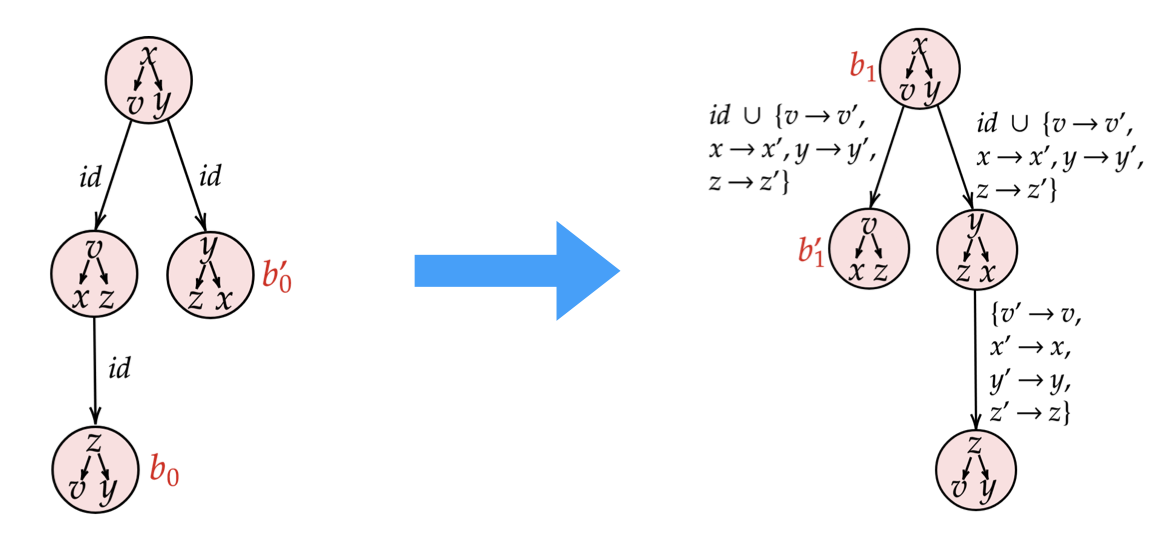
\includegraphics[scale=0.25]{figs/decomp1.png}
%	\end{center}
%	\caption{Figure shows circular doubly-linked list and its two tree decompositions. In the decompositions,
%                 the variables $v,x,y,z$ represent the nodes $1,2,3,4$ (in this order) of the list. We will show in Figures \ref{fig:decomp2}
%                 and \ref{fig:decomp3} that the right decomposition could be transformed to the left one.}
%	\label{fig:dll}
%\end{figure}
%\begin{figure}[t]
%	\begin{center}
%		\includegraphics[scale=0.25]{figs/decomp2.png}
%	\end{center}
%	\caption{The figure illustrates the reconnection operation. It shows the decomposition obtained by reconnection of the bag $b_0$ below the bag $b_0'$ in the right-handed side decomposition
%        of Figure \ref{fig:dll}. The figure also shows the primed variables introduced by the reconnection to prevent inference of reconnected pipes
%        with pipes along the reconnection path.}
%	\label{fig:decomp2}
%\end{figure}
%\begin{figure}[t]
%	\begin{center}
%		\includegraphics[scale=0.25]{figs/decomp3.png}
%	\end{center}
%	\caption{The figure illustrates the rotation operation. It rotates a path between the bags $b_1$ and $b_1'$ in the decomposition in Figure \ref{fig:decomp2}.
%        The operation changes orientation of edge between the two nodes and introduces the new primed variables for each existing variable,
%        e.g., $(x')'$ for $x'$ and since $x'$ already exists, $x''$ is created for $x$.}
%	\label{fig:decomp3}
%\end{figure}
\section{Representing Graphs with Trees and Tree Automata}
\begin{figure}[t]
\begin{center}
                \begin{subfigure}[b]{0.46\linewidth}
                  \includegraphics[scale=0.15]{figs/netys/dll.png}\\
                \end{subfigure}\\
		\begin{subfigure}[b]{0.32\linewidth}
		  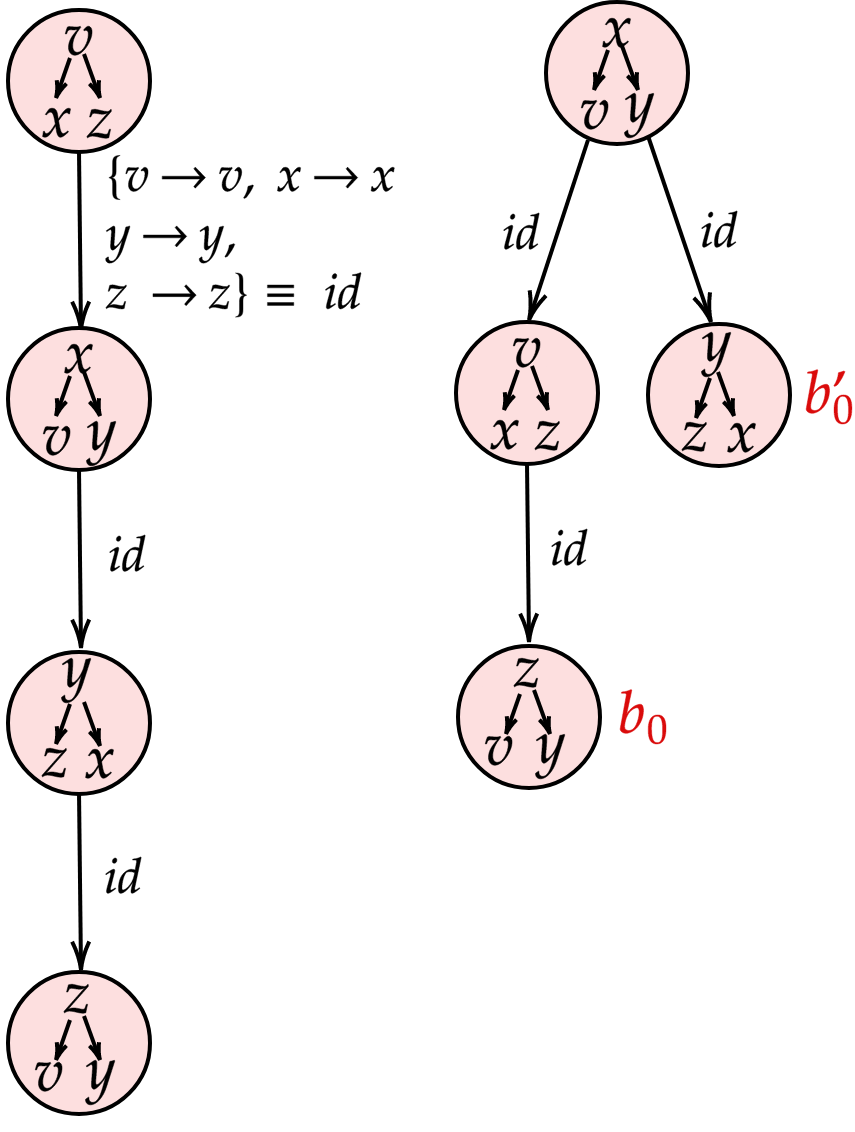
\includegraphics[scale=0.15]{figs/netys/decomp1.png}
                \end{subfigure}
		\begin{subfigure}[b]{0.33\linewidth}
		  \includegraphics[scale=0.15]{figs/netys/decomp2.png}
                \end{subfigure}
		\begin{subfigure}[b]{0.33\linewidth}
		  \includegraphics[scale=0.15]{figs/netys/decomp3.png}
                \end{subfigure}
\caption{Figure shows circular doubly-linked list (a) and its tree decompositions. In the decompositions (b),
        the variables $v,x,y,z$ represent the nodes $1,2,3,4$ (in this order) of the list.
        The figure shows that it is possible to transform the right decomposition in (b) to the left one using transformations shown in (c) and (d).
        Figure~(c) illustrates the reconnection operation. It shows the decomposition obtained by reconnection applied to  the right-handed side decomposition of (b)
        where the bag $b_0$ is reconnected below the bag $b_0'$.
        The~figure also shows the primed variables introduced by the reconnection to prevent inference of reconnected pipes
        with pipes along the reconnection path.
        Analogously, (d) show result of rotation applied to (c) where the bags $b_1$ and $b_1'$ were rotated.
        The operation changes orientation of edge between them and also introduces the new primed variables for each existing variable,
        e.g., $(x')'$ for $x'$ and since $x'$ already exists, $x''$ is created for $x$.}
\label{fig:decomps}
\end{center}
\end{figure}

We will first discuss encoding of graphs as variations on tree decompositions, similar to that used in \cite{iosif_treewidth_2013} and also \cite{iosif_deciding_2014}.
%The description should make it obvious that sets of such tree decompositions can be represented as finite tree automata.
% Our encoding of graphs into trees is based on the its treedecomposition.

A $\Sigma$-\emph{labeled graph} is a pair $g=(\vrts,\edgs)$
where $\vrts$ is a~finite set of nodes,
$\edgs\subseteq \vrts \times \Sigma \times \vrts$
is a set of $\Sigma$-labeled edges.
%\footnote{We might also want to add a node labeling function
%$\lab:\vrts\rightarrow\Sigma$, but we are omitting it for now for simplicity.}
%
A graph $g = (V,E)$ is \emph{deterministic} if for every node $n\in V$ and every label $a\in\Sigma$,
there is at most one node $n'\in\vrts$ such that $(n,a,n')\in\edgs$.
Unless stated otherwise, we will assume all graphs deterministic.

A \emph{tree decomposition} of a labeled graph $g$ over a finite set of variables $\vars$ and alphabet $\Sigma$
%of the graph $\gr$ 
is a~tree $\dect=(\bubbles,\edgs)$.
Nodes $\bubbles$ of $t$ are $\Sigma$-labeled graphs called \emph{bags}.
Nodes of a bag are variables from $\vars$. %, i.e., they are a set from $2^{\vars}$.
Edges of $\dect$ are labelled by partial mappings $\rho:\vars\rightarrow\vars$ called \emph{parameter assignments}.
%\footnote{we might want nodes \emph{labeled} by graphs instead of nodes being the graphs}
The \emph{tree-width} of a decomposition, $\treewidth \dect$, is the maximum cardinality of a parameter assignment in it.  %(+1?).
%Intuitively, the tree decomposition represents a graph which is constructed by merging the content of the bags, with the variable assignments specifying which variables of the neighbouring nodes correspond to the same graph node.
%This allows to recycle the same variable and use it to represent multiple graph nodes.
%%
%
A \emph{node occurrence} in $\dect$ is a pair $(x,\bag) \in \vars \times \bubbles$ where either $x$ is a node of a bag $\bag\in \bubbles$ (i.e., $x\in \bag$) (so called an \emph{active} occurrence) or $x$ belongs to the image of the parameter assignment on the edge targeting $\bag$ (then it is a \emph{passive} occurrence), i.e., $x\in img(\rho)$ such that $(\bag,\rho,\bag')$ is an edge of $t$ and $\rho$ is a label of the edge.
%
%A \emph{node occurrence} in $\dec$ is a pair $(x,n)$ where either $x$ is a node of a bag $n\in \bubbles$ (then it is an \emph{active} occurrence) or $x$ belongs to the image of the parameter assignment on the edge targeting $n$ (then it is a \emph{passive} occurrence).
%
The \emph{alias relation} $\sim$ is the smallest equivalence of occurrences such that if $(\bag,\rho,\bag')\in \edgs$ and $x' = \rho(x)$ then $(x,\bag)\sim(x',\bag')$.
%The transitive and reflexive closure $\sim^*$ of $\sim$ is called the \emph{alias relation}. 
%, the smallest equivalence on the set of all variable occurrences in $\dec$
%such that $(x,n)\sim(x',n')$ whenever $(n,\rho,n')\in \edgs$ and $x' = \rho(x)$.
%
%Intuitively, a pipe tracks a occurrences of the graph node through bags and parameter assignments in $\rho$.
%
The $\Sigma$-labeled \emph{graph represented by $\dect$} is the graph
%
$\gr^\dect = (\vrts^\dect,\edgs^\dect)$ 
%that, intuitively, arises by merging all graph bags at the aliasing nodes the pipes of $\dec$.
%Formally,
where the nodes $\vrts^\dect$ are the equivalence classes of $\sim$, called \emph{pipes},
and $\edgs^\dect = \{([(x,\bag)]_{\sim},a,[(x',\bag)]_{\sim}) \mid (x,a,x') \text{ is an edge of the graph } \bag\in \bubbles\}$ (that is, every edge $(x,a,x')$ of every graph $\bag\in \bubbles$ gives rise to\linebreak an edge $([(x,\bag)]_{\sim},a,[(x',\bag)]_{\sim})$ of the represented graph $\gr^\dect$).
%

An example of a graph (representing circular doubly-linked list data structure) and its tree decomposition is shown in Figure \ref{fig:decomps} (a) and (b).


We will work with the following restrictions of graphs and tree decompositions.
If a bag $\bag$ has an edge originating at $x$, then the pipe $[(x,\bag)]_{\sim}$ is \emph{allocated at $\bag$}.
%(in other words, allocated means that some the outgoing edges of $[(x,b)]_{\sim}$ is defined in $b$).
A \emph{backbone decomposition} corresponds to an (unoriented) tree backbone of the graph. 
It has three defining properties:
\begin{inparaenum}
\item
%
Every bag $\bag$ \emph{allocates exactly one graph node}. %\mh{which is said by the first restriction above?}
%
%If a node $n$ has an edge $(x,a,y)$, then we say that the pipe $[(x,b)]_{\sim}$ is \emph{allocated at $b$} 
%(in other words, allocated means that some the outgoing edges of $[(x,b)]_{\sim}$ is defined in $b$).
%
\item
Every graph node is \emph{allocated only once}.
\item
The tree is \emph{connected} in the sense that every tree edge corresponds to a graph edge (regardless the edge orientation).
That is, for every two adjacent bags,
%one of them has an edge incident with $x$ and the other has a graph node $y$ with $x = \rho(y)$ or $y = \rho(x)$.
one of them, say $\bag$, has an edge adjacent with $x$, and the other, $\bag'$, has an active occurrence $(\bag',z)$ with $(\bag,x)\sim (\bag',z)$.
%
\end{inparaenum}

%We discussed weaker versions of backbone decomposition, with relaxations that could have practical motivations.
%The first relaxation was to drop connectnes and replace it by something else. The motivation for that is, for instance, a natural separation-logic-encoding of a tree where all leaves point to the same predefined destination---this needs a disconnected decomposition.
%%
%Dropping the second condition should be also possible, a motivation for this might come from overlayed data structures or from biabduction, 
%where the special Mihaela weak separation star is used.


%Further, we say that a tree decomposition is \emph{connected} if all bags are connected graphs and every two adjacent bags encode at least one edge between their active occurrences, formally,
%one of them, say $b$, has an edge $(x,a,y)$, and the other, $b'$, has an active occurrence $(z,b')$ with $(x,b)\sim (z,b')$ or $(y,b)\sim(z,b')$.
%
%\footnote{We are discussing also a weaker restriction then connectedness, which would allow disconnected tree decompositions, but defining it requires work, so let's leave it as todo for now. The motivation for that is for instance a natural separation logic encoding of a tree where all leaves point to the same predefined destination---this needs a disconnected decomposition.}

Last, assuming a backbone decomposition, we define so called \emph{pipe child} relation $\rhd$.
Two pipes $p$ and $p'$ of a decomposition $\dect$ are in the relation $p \rhd p'$ iff $p$ is allocated in node $\bag$ and $p'$ in node $\bag'$
such that $(\bag,a,\bag') \in \edgs$ for some $a$.

%\paragraph{Tree Automata Representation.}
%\label{sec:TArepre}
%This is so far only an informal description.
A set of tree decompositions can be represented by a tree automaton. 
Intuitively, a node of a tree represents a node in the tree decomposition, and the label of each tree node records the bag and the labels on the decomposition edges leading from the node to its children. %The size of the alphabet is limited in terms of the maximal tree-width of the represented alphabet.
%

\section{Towards Entailment}
The idea for deciding entailment is to use tree automata language inclusion algorithms (such as \cite{tacas2010,almeida_reduction_2016,abdulla_computing_2008,libvata}) over tree automata encodings of tree decompositions.
The difficulty here is that a single graph has multiple decompositions and the tree automata may accept only some of them, hence simple language inclusion check may underapproximate the inclusion of sets of represented graphs (entailment).
%
We therefore propose means of saturating the tree automata languages with all possible tree decompositions of the represented graphs.
Conceptually, we will define a small set of operations which is \emph{complete} for tree decompositions, that is, allows to transform a decomposition into any other decomposition of the same graph.
%
The two tree automata under the entitlement accept decompositions with certain maximum tree width $t$, that can be easily determined.
%
The entailment procedure will apply the decomposition operations symbolically over the tree automata until they are saturated with all tree decompositions of the represented graphs with the tree width up-to $t$.
%
Computing the language inclusion of thus saturated automata is then a sound algorithm for entailment.


%In this section, we identify transformations of backbone decompositions which are \emph{complete}
%in the sense that they allow one to freely move between any two equivalent tree decompositions.
%We will concentrate on showing the result for local star connected decompositions only,
%hence, unless said otherwise, decomposition in this section are assumed star local connected.

We will now outline the operations. These operations are essentially meant to complete the \emph{rotation} operation of \cite{IosifRogalewiczVojnar:deciding}.

\begin{comment}
\subsection{Decomposition Isomorphism}
We will use a definition of equivalence of two tree decompositions little weaker and more technical than simple isomorphism of represented graphs.
%
Firstly, we want to reason modulo useless appendices of pipes: pipes that continue down some branch of the decomposition in which there is actually no active occurrence of the pipe.
%
We assume that removing the pipe appendices can be handled somehow even on a tree automata representation of sets of decompositions. \footnote{TODO: Should the definition of tree-width ignore pipe appendices? Might be important in the context of the Lemmas about phases further.}
%
We also want to reason modulo renaming of variables that preserve the important structure of the decomposition. %We also think that renaming of variables can be handled somehow.
%
Therefore, we will consider two decompositions \emph{isomorphic} if after removing the redundant variable occurrences,
they are equal up to \emph{decomposition isomorphism}:
%
a decomposition isomorphism between two tree decompositions $\dect$ and $\dect'$ consists
of two mappings $f$ and $g$ where $f$ is a graph isomorphism between their nodes (from nodes of $\dect$ to nodes of $\dect'$),
and $g$ is a bijection between their pipes (nodes of the represented graph) such that a bag $n$ of $\dect$ encodes a graph edge $(p,a,p')$  (edge between pipes) if and only if $f(n)$ encodes the edge $(g(p),a,g(p'))$.
%
Notice that the particular names of variables do not play a role in the definition of decomposition isomorphism as far as the same graph bags encode the same graph edges.
%
\begin{lemma}
Isomorphic decompositions encode isomorphic graphs.
\end{lemma}
%
%Formally, homomorphic renaming of variables is a mapping $f$ that maps every occurence of a variable to a variable. Then, for a graph bubble $n$, $f(n)$ is the graph-homomorphic image of $n$ under the graph homomorphism $f_n$ such that $f_n(x) = f(x,n)$, and we require that it is actually a graph somorphism, and for every edge $e = (n,\rho,n')$, $f_e = (f_n(n),f_e(\rho),f_{n'}(n'))$ where $f_e(\rho)$ is the mapping that contains $f(x,n)\mapsto f(y,n')$ for every $x\mapsto y \in \rho$ such that $(x,n)$ and $(y,n')$ are variable positions. This is an ugly definition.
%
In order to show that a particular set of decomposition operations is complete,
we argue that
%
the equivalence classes of the decomposition isomorphism may be characterised by the \emph{pipe child relation}.
%
Namely, in a backbone decomposition, a pipe $p$ of is a \emph{child of pipe} $p'$ if the allocating bag of $p$ is a child of the allocating bag of $p'$.

\begin{lemma}
Two backbone decompositions are isomorphic iff their child relations are isomorphic (under a standard isomorphism of relations).
\end{lemma}
\end{comment}

%\paragraph{Operations}
%The two basic operations we were thinking about are \emph{subtree reconnection} and \emph{rotation}. The subtree reconnection is allowed to reconnect a subtree below some of the peers of its root. The rotation is the one from the paper of Adam, Radu, and Tomas \cite{IosifRogalewiczVojnar:deciding}.
%Ultimately, we will want to implement an unbounded number of these operations on an infinite set of decompositions represented by a tree automaton.

%We note that we are not entirely sure about what the needed set of operations is so far.
%We are also thinking about a more complex variant of reconnection which allows reconnecting of a subtree below its ancestor or predecessor too, maybe this operation alone could be enough.
%
%\footnote{but maybe not, for instance things like moving between the two symmetrical encodings of a DLL seem problematic.}


%\begin{description}[style=unboxed,leftmargin=0cm]
\begin{description}[leftmargin=2mm]
%\paragraph{Reconnection.}
\item[Reconnection.]
The operation of reconnection is parameterised by two \emph{peer} bags $\bag$ and $\bag'$ of the decomposition that allocate pipes $p$ and $p'$, respectively (they are peer bags, i.e. not on the same branch of the tree).
Its purpose is to create an equivalent decomposition with the child relation on graph nodes being the same up to that $p$ becomes a child of $p'$ in the new decomposition.


The operation is implemented as a function $\chr(\bag,\bag',\dect)$ that transforms a tree decomposition $\dect = (\bubbles,E)$ into $\dect'$ as follows.
First, the pipes that are reaching $\bag$ in $\dect$ must be in $\dect'$ sent to $\bag'$ through the path between $\bag$ and $\bag'$, called the \emph{reconnection path}.
Let $\rho_1,\ldots,\rho_k$ be the sequence of edge labels appearing on the reconnection path.
%
Take every label $\rho_i$ of an edge on the reconnection path with $2 < i \leq k$, and replace it by $\rho_i' = \rho_i \cup \{x'\mapsto x'\mid x\in \img(\rho_1)\}$.
The primed variables must be such that they do not appear anywhere on the reconnection path, neither in the graph bags nor in the variable renamings (they may be fresh variables).
%
This is to stretch the pipes reaching $\bag$ through the reconnection path towards $\bag'$.
%
Replace also $\rho_2$ by $\rho_2' = \rho_2\cup \{x'\mapsto y\mid \rho_1(y) = x\}$.
This binds the new primed part of the pipes with the original pipes reaching $n$.
%
Last, replace the edge leading to $\bag$ by $(\bag',\rho_1',\bag)$ where $\rho_1' = \{x'\mapsto x\mid x\in \img(\rho_1)\}$.
%
This makes $\bag$ a child of $\bag'$ and connects the new primed pipes to the corresponding original pipes of $\bag$.

An example of the operation is shown in Figure \ref{fig:decomps} (c)
where the righ-handed side decomposition $\dect_0$ from Figure \ref{fig:decomps} (b) is rotated by $\chr(b_0,b_0',\dect_0)$.
%\paragraph{Complex reconnection.} 
%\item[Complex reconnection.] 
%It is a variant of the reconnection where $\bag$ and $\bag'$ can be on the same branch. The normal reconnection on $\bag$ and $\bag'$ would in such case introduce a cycle,
%which the complex reconnection must break, either by some predefined way depending on $\bag$ and $\bag'$ or according to a third parameter, a node on the path between $\bag$ and $\bag'$.

%\paragraph{Rotation.}
\item[Rotation.]
%From Adam, Radu, Tomas paper \cite{IosifRogalewiczVojnar:deciding}.
The rotation operation is parameterised by two bags $\bag$ and $\bag'$ of the decomposition. The operation inverts the edges in the path $\pi$ between $\bag$ and $\bag'$.
Then it redirects the incoming edge of $\bag$ to $\bag'$.
Intuitively, it takes a subtree with the root $\bag$, changes the root to $\bag'$ and inverts the edges in the subtree. 
It yields an equivalent tree decomposition with respect to child relation which is inverted between pipes allocated in the nodes of the path $\pi$.

The operation is implemented as a function $\rot(\bag,\bag',\dect)$. At the tree level, it works as follows.
Consider the path $\pi:\bag=\bag_1,\ldots,\bag_n=\bag'$. Remove each edge $(\bag_i,\rho,\bag_{i+1})$, where $1\leq i \leq n$, between nodes in $\pi$
from $\edgs$ and add $(\bag_{i+1},\rho,\bag_i)$ to $\edgs$.
Moreover, we replace the edge $(m,\rho,\bag)\in\edgs$ by the edge $(m,\rho,\bag')$ to $\edgs$.
The labels along the rotated path are changed in the following way.
Replace the label $\rho_1$ of the edge $(m,\rho_1,\bag')$ by $\rho_1 = \{x\mapsto x'\mid x \in \dom(\rho_1)\}$.
Replace each label $\rho_i$ in the path $\pi$ by $\rho_i=\rho_i\cup \{x'\mapsto x'\mid x' \in \img(\rho_1')\}$ for $2 \leq i \leq \bag$.
Finally, replace the label $\rho_\bag$ over the edge leading to $\bag$ by $\rho_\bag'=\rho_\bag\cup\{x'\mapsto x\mid x' \in \img(\rho_1')\}$.

An example of the operation is shown in Figure \ref{fig:decomps} (d) where the decomposition $\dect_1$ from Figure \ref{fig:decomps} (c) is rotated by $\rot(b_1,b_1',\dect_1)$.

%\paragraph{Phase.}
\item[Phase.]
%We will continue with the assumption that a complete set of operations is rotation and (normal) reconnection.
The operations from one tree decomposition to an equivalent one may take unboundedly many operations. We will devide them into \emph{phases}.
%We will therefore need a procedure that implements unboundedly many operations on a tree automaton that represents infinitely many decompositions in a finite way.
%To make this procedure manageable, we will divide it into \emph{phases}.
One phase can still perform unboundedly many operations, but the set is restricted: 
the reconnection paths of all reconnections must be node disjoint.
%This restriction will make the implementation on tree automata manageable, as we will discuss later.
%We will then that a constant number of phases is always enough if we only need isomorphic decompositions \emph{up to a given fixed tree-width}.

Formally, a phase is characterised by a set of operation parameters, pairs of nodes $\{(\bag_1,\bag'_1),\ldots,(\bag_k,\bag'_k)\}$ of a decomposition $\dect$
such the for any two $1\leq i,j\leq k, i\neq j$, the operation paths between $\bag_i$ and $\bag_i'$ and between $\bag_j$ and $\bag_j'$ are node disjoint.
A result of the phase is any decomposition which arises by performing the appropriate operation on $(\bag_i,\bag_i')$ for each $i$ (in any order).

An example of two phases are show in Figures \ref{fig:decomps} (c) and (d) where the right-handed side decomposition from Figure \ref{fig:decomps} (b)
is transformed in the left-handed side decomposition of the same figure in these two phases.
\end{description}

An important consequence of the disjointness of the reconnection paths is that all the operations can be implemented
while only doubling the number of variables and the tree-width of the original decomposition.
Particularly, all the operations can use the same set of fresh primed versions of the variables $\vars$ on the operation path without fearing a conflict with the names of the existing pipes.
%
\begin{lemma}
\label{lemma:vars}
One phase at most doubles the number of variables.
\end{lemma}

%We then conjecture that to saturate a tree automaton with all decomposition of the represented graphs up to certain tree-width,
%we need only finitely many phases.
%
%
%That would mean that to decide entailment of two tree automata representations, saturating them with all decpompositions up to their maximum tree-width would take a number of phases dependent on the maximum tree width. 
We conjecture that the number of phases needed depends on only on the tree-width:

\begin{conjecture}
An equivalent decomposition $\dect'$ can be obtained from $\dect$ in a number of phases that depends only on $\max(\treewidth \dect,\treewidth {\dect'})$.
\end{conjecture}

%The following lemma is crucial, we need a proof.
%\begin{lemma}
%\label{lemma:phases}
%An equivalent decomposition $\dec'$ can be obtained from $\dec$ in at most $\max(\treewidth \dec,\treewidth {\dec'})$ phases.
%\end{lemma}
%\begin{proof}
%\end{proof}
%
%\begin{lemma}
%\label{lemma:phasecost}
%Let $MTW = \max(\treewidth \dec,\treewidth {\dec'})$.
%$t'$ will
%have at most $|\vars|*2^{MTW}$.
%% and also $\treewidth{t'}\leq \treewidth{t}*2^{MTW}$
%\end{lemma}
%\begin{proof}
%It follows from Lemma \ref{lemma:phases} that
%every phase doubles the number of variables, hence there is
%$|\vars'| \leq |\vars|*\underbrace{(2*\ldots *2)}_{MTW} =  |\vars|*2^{MTW}$.
%\end{proof}

%\paragraph{Implementation of Phase over Tree Automata.}
%
%The main result here should be that a phase can be implemented on a tree automaton,
%with a size blow-up exponential only to the number of variables or to the maximum tree-width of a represented decomposition.
%
Next, we discuss implementation of a phase
over tree automata (TA) representation.
% A phase can be implemented over the tree automata representation.
%That is, there is an effective tree automata transformation, called \emph{automata phase},
We design phase over TA in such way that its results is an automaton that encodes all possible results of phase applied at any possible decomposition represented by the original automaton.
%
We will briefly sketch the basic idea of the operation. %This operation is exponential only to the maximum tree-width of a represented decomposition.

Namely, saturation with reconnections can be implemented by a tree transducer.
Seen as a top-down machine, it oscillates between two routines, \emph{idle},  and \emph{reconnecting}.
In the idle state, it is just traversing the tree. At any node $r$, it may non-deterministically chose to start reconnecting. 
When reconnecting, it non-deterministically selects two peer descendants of $r$, nodes $\bag$ and $\bag'$, and performs the reconnection on them. 
The reconnection, roughly, involves adding of primed versions of existing pipes on the path from $\bag$ to $\bag'$ and reconnecting the subtree of $\bag$ below $\bag'$. 
%All this a transducer can do. 
After that, the reconnecting phase stops and the transducer continues traversing the tree in the idle phase. The requirement in the definition of phase on the disjointness of the reconnection maths makes this doable---when reconnecting, the transducer needs to worry only about one reconnection path at a time.
Saturation with rotations can be then implemented similarly as in \cite{iosif_deciding_2014}.
%

We conjecture, based partially on Lemma~\ref{lemma:vars}, that such implementation of a phase over tree automata representation is cheap:
\begin{conjecture}
The implementation of a tree automata phase at most doubles the number of variables and leads to an automaton that is of a polynomial size assuming a fixed tree-width of the original automaton.
\end{conjecture}


Based on Conjecture 1 and 2, the saturation of a tree automata representation with all decompositions until a fixed tree-width $t$ can be done in a time that is polynomial (when the $t$ is fixed).
%
Recall that deciding entailment between two TA representations, we saturate both of them up to the maximum tree-width $t$ (in fact, it is enough to use the maximum tree with of the automaton that is supposed to entail),
and then we compute language inclusion between the saturated automata.
%
Since language inclusion of tree automata is EXPTIME-complete, Conjectures 1 and 2 give an entailment algorithm singly exponential, assuming a fixed maximum tree-width $t$.

\section{Conclusions and Future Work}
We have presented basic outline of a formalism for representing shape graphs based on tree automata. The ideas should lead to an entailment algorithm, and conjectures that, if true, would imply that the algorithm is relatively fast assuming fixed maximum tree-width of the graph representations.

We plan to perfect these ideas and to prove Conjectures 1 and 2. The conjectures are somewhat optimistic, but not in a direct contradiction with the recent 2-EXPTIME-hardness result of \cite{Iosif:LPAR}. If the conjectures turn out to be false, we wish to search for (1) restrictions under which they are true, and/or (2) to prove termination of the described entailment algorithm regardless its complexity.
Our long term plan is to develop a shape analysis framework based on this formalism and entailment check in the spirit of \cite{holik_boxes_2013} and also \cite{locle:secondorder}.

%their saturation is polynomial with a fixed maximum tree-width. Since tree automata inclusion is EXPTIME-complete, the entailment would be fixed parameter EXPTIME-complete with the parameter being the maximum tree-width. 
%
%
%Since the tree width of the decomposition we need to obtain is supposed to be bounded, we need only a bounded number of phases. The resulting automaton can be exponentially large, but with only the tree-width of the original in the exponent. 
%, and since the automata grow only polynomialy with each phase (as we outline in Section~\ref{sec:TArepre}, 
%their saturation is polynomial with a fixed maximum tree-width. Since tree automata inclusion is EXPTIME-complete, the entailment would be fixed parameter EXPTIME-complete with the parameter being the maximum tree-width. 



%
%\tv{Define the notion of TA used. What is $R$?}
%
%Consider a tree decomposition $\dec=(\vrts,\edgsdec,\tagal,\lab)$ of a graph
%$\gr$.
%%
%Then a run of $\ga$ over $\dec$ is a mapping $\rho: \vrts \rightarrow Q$ such
%that $\rho$ is a valid run of $\fta$.
%We will denote domain of run by $\dom$ and its image by $\img$.
%
%\tv{Define the graph language of $\ga$.}
%
%We introduce an operation for pumping transitions to the graph automaton.
%Consider a graph automaton $\ga= (Q, \tagal, \delta, R, \vars)$ having
%a graph $\gr$ in the graph language, we will add to this automaton
%the new transitions and create $\ga'= (Q', \tagal', \delta', R', \vars')$
%which language contains all possible tree decompositions $\dec'$ of $\gr$.
%The so called \emph{pumping algorithm} is the following
%
%\begin{enumerate}
%        \item Copy each component of $\ga$ to $\ga'$, i.e., $Q'=Q, \tagal'=\tagal, \delta'=\delta, R'=R, \vars'=\vars)$.
%	\item Generate different roots - Nondeterministically choose a state $q\in Q$ s.t. $q\not\in R$ and
%              add it to $R'$, i.e., $R'=R\cup Q'$ such that $Q'\subseteq Q$.
%              Change each $\gtrans{q}{(a,V,v)}{q_1,\ldots,q_n}\in \delta$ to $\gtrans{q}{(a,V,v,new)}{q_1,\ldots,q_n}$, i.e.,
%              $\forall q \in Q': \gtrans{q}{(a,V,v)}{q_1,\ldots,q_n}\in \delta \rightarrow \gtrans{q}{(a,V,v,new)}{q_1,\ldots,q_n}\in \delta'$.
%              Nondeterministically choose a state $r \in R$ and add a transition $\gtrans{r}{(a,V,v,ex)}{r_1,\ldots,r_n}$ to $\delta$
%              for each $\gtrans{r}{(a,V,v)}{r_1,\ldots,r_n}\in \delta$, i.e., $\exists r\in R: \gtrans{r}{(a,V,v)}{r_1,\ldots,r_n}\in \delta
%              \rightarrow \gtrans{r}{(a,V,v,ex)}{r_1,\ldots,r_n} \in \delta'$.
%	\item Choose nondeterministically a transition $\gtrans{q}{(\nul,\_,v)}{} \in \delta$ and
%              add transition $\gtrans{q}{(a,\_,v_i,p\rightarrow q)}{q_1, \ldots,q_n}$ to $\delta'$ for each $\gtrans{p}{(a,\_,v)}{q_1,\ldots,q_n}\in \delta$
%              where $i\in\mathbb{N}$ is a nondeterministically chosen index.
%              Also nondeterministically choose a transition $\gtrans{q}{(a,V,v)}{q_1, \ldots,q_n} \in \delta$ and add $\gtrans{q}{(\nul,V,v_i,q\rightarrow\nul)}{}$
%              to $\delta'$ where $i\in\mathbb{N}$ is an index.
%        % \item Choose nondeterministically a transition $\gtrans{p}{(a,V,v)}{q_1,\ldots,q_n}$ and add $\gtrans{p}{(a,V',v,V\rightarrow V')}{q_1,\ldots,q_n)}$
%        %      to $\delta'$. Reindex variable in another transitions if needed \textbf{TODO: define reindexing}.
%\end{enumerate}
%
%Consider the tree decompositions $\dec'=(\vrts',\edgsdec',\tagal',\lab')$ accepted by the resulting automaton $\ga'$
%and the original tree decompositions $\dec=(\vrts,\edgsdec,\tagal,\lab)$. % via run $\rho$.
%The following conditions need to be satisfied:
%\begin{enumerate}
%        \item The root $r$ of $\dec'$ is
%              labelled by a label with the $new$ sign in (i.e., a newly
%              generated root was used) iff there is a (exactly one) node $n$
%              with label containing the $ex$ sign (a transition which was used to accept
%              root for the original tree decomposition).
%              Formally,$(\exists r\in N': r\emph{ is a root } \wedge new \in r_{\sa}) \rightarrow
%              (\exists n\in \vrts': ex \in n_{\sa})$.
%	% \item If there is a node $n$ in $\dec'$ such $p\rightarrow q$ is in a label of $n$ then
%              % there is a node $n'$ in $\dec'$ with $p\rightarrow\nul$.
%              % Moreover it holds that no other $n''$ in $t'$ with $p\rightarrow q$ sign in a label.
%              % It also holds that $n_{\va_i}=v \wedge n_{\va_i}=n_{\va}'$ and for each node $m$ in the path between $n$ and $n'$ holds
%              % that $n_{\va_i}\not\in m_{\vqa}$.
%
%              % If there is a transition $r: \gtrans{q}{(\_,\_,v_i,p\rightarrow q)}{q_1, \ldots,q_n}$ in $s$
%              % then there has to be $r':\gtrans{p}{(\_,\_,v_i,p\rightarrow\nul)}{}$ in $s$.
%              % Moreover it holds that $r$ and $r'$ is in $s$ just once.
%              % Consider a node $n$ from the tree decomposition $\dec'$ such that $\rho(n) = q$ created by application of $r$ and $n'$ such that $\rho(n') = p$ by application of $r'$.
%              % Then $n_{\va_i}=v \wedge n_{\va_i}=n_{\va}'$ and for each node $m$ in the path between $n$ and $n'$ holds
%              % that $n_{\va_i}\not\in m_{\vqa}$.
%        \item Consider a tree decomposition $\dec'$ accepted by $\ga'$ and
%              the original decomposition $\dec$.
%              % The run $\rho$ provides us with information to renconstruct the original decomposition $\dec$.
%              It must hold that each $n\in\vrts$ has to be in the same equivalence class either for $\dec$ or $\dec'$.
%	      \textbf{TODO: algorithm for reconstruction of the original $\dec$}.
%              Consider the following transducers:
%              \begin{itemize}
%                \item $\tds_o$ is a marking transducer which nondeterministically choose two nodes, both with the same identifying variable $y$ and mark them by $\omark$.
%                \item $\tds_p$ nondeterministacally choose two nodes $n$ and $n'$ with the identifying variable $x$.
%                               The node $n$ is labelled by a label with sign $p\rightarrow q$ and is called a start of jump.
%                               The node $n'$ is labelled by $p\rightarrow \nul$ and is called an end of a jump.
%                               Then it checks the following things:
%                  \begin{itemize}
%                    \item No other node labelled with a jump mark is in the path between $n$ and $n'$,
%                    \item checks whether there is no $x$ in $m_\vqa$ for any $m$ in the path between the chosen nodes,
%                    \item between $n$ or $n'$ and any other node labelled by $p\rightarrow q$ or $p\rightarrow \nul$ is a node $m$ such that $x\in m_\vqa$.
%                  \end{itemize}
%                       If the conditions are satisfied, then it reconnects the jumped part of graph to its original place and
%                       remove $p\rightarrow q$ or $p\rightarrow \nul$ marks.
%               \item $\tds_t$ Checks whether there is no $y$ in $m_\vqa$ for any $m$ in path between the nodes with $\omark$ and remove $\omark$.
%              \end{itemize}
%          Consider the following automata:
%\begin{itemize}
%		 \item Automaton $\autn$ accepts tree decomposition if that there is no $y$ in $m_\vqa$ for any $m$ in path between the nodes with $\omark$
%		 \item Automaton $\auto=\tds_t\circ(\tds_p\cup id)^{tw}$, where $tw$ is a number denoting tree width.
%              \end{itemize}
%               Then consider the following automaton $\ga_{wrong}= ((\overline{\autn} \cap \auto)\cup (\autn \cap \overline\auto)) \circ \tds_o$.
%               Then once we substract the language of $\ga_{wrong}$ from the language of the pumpped automaton $\ga'$ we obtain a language
%               (and its represnting automaton) satistfying the condition mentioned in this item.
%\end{enumerate}

%\section{Related work}

%To proceed:
%\begin{description}
%  \item \cite{Courcelle} Courcelle
%    \begin{description}
%      \item \emph{What?} The original Courcelle theorem claiming that any graph property definable in MSO can be decided in linear time on graphs of bounded treewidth.
%    \end{description}
%  \item \cite{iosif_treewidth_2013} Adam, Jirka, Radu
%    \begin{description}
%      \item \emph{What?} They prove decidability of satisiability and entailment for separation logic capable to describle recursive data structures such as SLL, DLL, tree.
%       The proof is done by reduction to MSO over bounded tree width. 
%    \end{description}
%  \item \cite{IosifRogalewiczVojnar:deciding} Adam, Tomas, Radu
%    \begin{description}
%      \item \emph{What?}  It uses reduction to tree automata to decide entailment of fragment of separation logic describing recursive structures with local edges w.r.t. spanning tree.
%        Using the reduction, the entailment problem is EXPTIME-complete.
%        It solves the problem that the same recursive structure may be represented differently from the different views by introducing closure operation on tree automata
%        which closes a tree automaton representing all different rotations of spanning trees in its language.
%    \end{description}
%  \item \cite{Katelaan:seplog,pagel} Jens and Florian
%    \begin{description}
%      \item \emph{What?} They provide a decision procedure for separation logic with user-defined predicates describing graphs of bounded tree width.
%         The procedure works without reduction to MSO over graphs with bounded tree width and has double-exponential upper bound w.r.t. to size of the formula.
%         In \cite{pagel} the procedure was made sound. Their fragment of separation logic allows "conjunction, disjunction, guarded forms of negation, septraction,
%         and the magic wand in addition to the separating conjunction.
%    \end{description}
%  \item \cite{Iosif:CSL,Iosif:LPAR} Radu the last papers
%    \begin{description}
%      \item \emph{What?} These work further develop previous work of Radu Iosif \cite{CADE-24,IosifRogalewiczVojnar:deciding}. Now, he finally managed to get rid off czech scum.
%        The works show that the entailment for sepration logic over inductively defined predicates (describing pointer-linked data structures) is simply exponential w.r.t.,
%        the number of symbolic heaps and doubly exponential w.r.t. the maximal size among symbolic heaps in the input entailment. It generalise the fragment of the seperation logic
%        from  the previous works
%        \cite{CADE-24,IosifRogalewiczVojnar:deciding,Katelaan:seplog} to equationally restricted formulas. Particulary it enables entailment over forest-like heap structures
%        instead of single trees.
%    \end{description}
%      \item Separation logic overview
%    \begin{description}
%      \item \emph{What?} Seperation logic (SL) was introduced as an extension of Hoare logic for reasoning about mutable data structures by John Reynolds \cite{Reynolds:SepLogic:02}.
%        Later, it was shown that entailment of SL formulas is generally undecidable \cite{SL-overview} (an overview paper).
%      \item However, there are decidable fragments of SLL. One of them is restriction of SL to reason only about SLL \cite{berdine} (Ohearn paper on SLL) which the paper proved to be
%        in co-NP. This work later lead to a development of industry used tool \cite{infer} (infer).
%      \item The previous work was further refined by \cite{CONCUR11} (Cook et al.) providing algorithm for entailment in PTIME which works by a reduction of entailment to graph
%        homomorphism.
%      \item Finally, \cite{ESOP13} (Mihaela and Constantin) generalizes decidable fragment of SL to nested and overlaid structures and provides with a decision procudere in co-NP.
%    \end{description}
%\end{description}

\chapter{Shape Analysis based on SMT Solving}
\label{ch:fmcad}
Apart from automata based approach the author of this thesis participated in work on shape analysis
based on SMT solving.
Although we are not the main authors and have a rather minor share in this work (published in \cite{fmcad18})
we add it here to give another perspective on shape analysis.
We provide with an overview of the approach. For a full technical description please check \cite{fmcad18}.

The verification method is based on describing state space of a program w.r.t. to a property of interest
using system of logic formulae and so called templates which describes state space of program using SMT solver.
The templates are special logic formulae and are conceptually similar to abstract domain
in abstract interpretation.
They are manually crafted to capture only certain aspects of an analysed program
what makes analyses computationally feasible.
Therefore we call templates (abstract) domains in the rest of the chapter.

The main contributions of this work are:
\begin{compactenum}
\item We propose a novel abstract template domain for reasoning over
  heap-allocated data structures such as singly and doubly linked
  lists using a template-based parameter synthesis engine.
\item Since we designed our domain in existing framework for template-based
  verification we can build product and power domain combinations
  of our heap domain with structural domains (e.g.\ trace partitioning) and
  value domains such as template polyhedra that capture the content of
  data structures.
\item We implement our abstract heap domain in the 2LS verification
  tool for C~programs. We demonstrate the power of the proposed domain
  on benchmarks, which require combined reasoning about
  the shape and content of data structures, showing that other tools, which
  performed well in SV-COMP, cannot handle these examples.
\end{compactenum}

In this chapter, we firstly describe the verification method and then the domain for shape
analysis which we designed.

\section{Template-based Program Verification}

In template-based program verification, 
a state of a program is a logical interpretation of logical variables
corresponding to each program variable. A set of states can be described using
a formula---states in the set are defined by models of the formula. Given a
vector of variables $\vx$, the predicate $\fminit(\vx)$ describes
the initial states. A transition relation is described as a formula
$\fmtrans(\vx, \vxp)$.

From these, it is possible to determine the set of reachable states as the
least fixed-point of the transition relation starting from the states described
by $\fminit(\vx)$. This is, however, difficult to compute, so instead, we use an
\emph{inductive invariant}.
A verification task requires showing that the set of reachable
states does not intersect with the set of error states $\err(\vx)$.
Using the concept of inductive invariants and  existential second-order
quantification ($\exists_2$), we can formalise it as:
\begin{equation}\label{eq:2ls}
\begin{split}
\exists_2 \inv . \; \forall \vx, \vxp . \; 
& (\fminit(\vx) \Longrightarrow \inv(\vx)) \; \wedge \\ 
& (\inv(\vx) \wedge \fmtrans(\vx,\vxp) \Longrightarrow \inv(\vxp)) \; \wedge \\
& (\inv(\vx) \Rightarrow \neg Err(\vx))
\end{split}
\end{equation}

The above equitation would need a solver able to deal with second-order logic quantification,
however, there are currently no general and efficient solvers able to do it.
Therefore we reduce the problem to iterative application of a first-order solver
by restriction of inductive invariant $\inv$ to $\templ(\vx, \vdelta)$ where $\templ$ is
a fixed expression (a so-called \emph{template}) over program
variables $\vx$ and template parameters~$\vdelta$.
Template captures only properties of interest for a certain analysis (which corresponds
to choice of an abstract domain in abstract interpretation).
The resulting first order search is following:
\begin{equation}\label{eq:formula-templates}
\begin{split}
\exists \vdelta . \; \forall \vx, \vxp . \; & 
(\fminit(\vx) \Longrightarrow \templ(\vx, \vdelta)) \; \wedge \\ 
& (\templ(\vx, \vdelta) \wedge \fmtrans(\vx,\vxp) \Longrightarrow 
\templ(\vxp, \vdelta))
\end{split}
\end{equation}

Finally, since quantifier alternation is a problem for current SMT solvers
we iteratively search for the negated formula:
\begin{equation}\label{eq:templ_neg}
\begin{split}
\exists \vx, \vxp .\; &
    \neg (\fminit(\vx) \Longrightarrow \templ(\vx, \vd)) \; \vee \\
& \neg (\templ(\vx, \vd) \wedge \fmtrans(\vx,\vxp) \Longrightarrow \templ(\vxp, \vd))
\end{split}
\end{equation}

\subsection{Program Encoding}
We encode the program into a formula representing a specific \emph{static single assignment form} (SSA).
As usual, we use a fresh copy~$x_i$ of each variable~$x$ for each program location~$i$
where the value of~$x$ is modified.
In this encoding, special variables called \emph{guards} are used to track the control flow of the program
in such way that for each program location~$i$ there is a~Boolean variable~$\ssag{i}$ which value
encodes whether the program location is reachable.

To achieve acyclicity of the SSA, we cut the path coming from the end of the loop.
We then represent the value of each variable $x$ at the loop head using a
\emph{phi variable} $x^{phi}$ whose value is defined by a non-deterministic
choice between the value coming from before the loop, say $x_0$, and the
value coming from the end of the loop. The latter value is represented by a
newly introduced \emph{loop-back} variable $x^{lb}$. In particular, we let
$x^{phi} = g^{ls} ~?~ x^{lb} : x_0$ where $g^{ls}$ is a so-called
\emph{loop-select} Boolean guard that is unconstrained in order to model the
non-deterministic choice. 
The effect of the loop is overapproximated and 
the value of the loop-back variable $x^{lb}$ is initially unconstrained
and later constrained by the derived candidate loop invariants

\section{Template domain for Shape Analysis}
We design a template domain which are used in the described framework to
derive \emph{loop invariants} of the analysed programs.
Templates are also used to constrain values of the \emph{loop-back variables} that are
used in the SSA-based program encoding to over-approximate values returning from
the end of the loop to the loop head.
%
Since we are interested in describing shapes of heaps,
we limit our shape domain to the set $\ptrlb$ of all \emph{loop-back pointers}. 
%
Let $L$ be the set of all loops in the program. 
%
Since there is one loop-back pointer variable for each pointer variable and
each loop, we define $\ptrlb = \ptr \times L$.
%
We denote elements $(p, l) \in \ptrlb$ by $\ssaplb{i}$ where $i$ is the program
location of the end of the loop $l$.
%
Intuitively, the value of $\ssaplb{i}$ is an abstraction of the value of the
pointer $p$ coming from the end of the body of the loop $l$.
%
The property that our base shape domain describes is the
\emph{may-point-to} relation between the set $\ptrlb$ and the set
$\addr$ of memory addresses.

The template of our base shape domain has the form of the formula:
\begin{equation}\label{eq:templ_shape}
\begin{split}
\templ^S \equiv \bigwedge_{\ssaplb{i} \in \ptrlb}
\templ^S_{\ssaplb{i}}(d_{\ssaplb{i}}).
\end{split}
\end{equation}
%
It is a conjunction of so-called \emph{template rows} $\templ^S_{\ssaplb{i}}$,
each row corresponding to one loop-back pointer from the set $\ptrlb$.
%
A template row $\templ^S_{\ssaplb{i}}(d_{\ssaplb{i}})$ describes the
may-point-to relation for the loop-back pointer $\ssaplb{i}$.
%
The parameter $d_{\ssaplb{i}} \subseteq \addr$ of the row (a~so-called
\emph{abstract value of the row}) specifies the set of all addresses from the
set $\addr$ that $p$ may point to at the location $i$.
%
The template row can thus be expressed as the quantifier-free formula:
\begin{equation}\label{eq:templ_row}
\begin{split}
\templ^S_{\ssaplb{i}}(d_{\ssaplb{i}}) \equiv (\bigvee_{a \in
d_{\ssaplb{i}}} \ssaplb{i} = a)
\end{split}
\end{equation}
  
Abstract values of template rows corresponding to pointer fields of abstract
dynamic objects allow the domain to describe unbounded linked paths in the heap,
such as list segments.

In order to use the base shape domain in our approach, we have to augment it
with information about the guard variables that encode the program's control
flow in the SSA. The guards express when an appropriate loop-back control edge
is executed and the loop-back pointer has a defined value\footnote{Using the base domain without the guard variables would be sound. However, it
would produce very imprecise results since the abstract value would
need to cover even states in which the loop-back edge was not taken.}.
%
A row of a \emph{guarded shape template} is defined
as a formula:
\begin{equation}\label{eq:templ_row_guard}
\begin{split}
\templ^G_{\ssaplb{i}}(d_{\ssaplb{i}}) \equiv G_{\ssaplb{i}}
\Rightarrow \templ^S_{\ssaplb{i}}(d_{\ssaplb{i}})
\end{split}
\end{equation}
where $G_{\ssaplb{i}}$ is a conjunction of SSA guards associated with the definition of the variable
$\ssaplb{i}$ and $\templ^S_{\ssaplb{i}}$ is as in the base shape domain.
%
If $G_{\ssaplb{i}}$ is true for a program run, the definition of $\ssaplb{i}$
was reached in the run.
%
A shape template $\templ^G$ with guards is then a conjunction:
\begin{equation}\label{eq:templ_guard}
\begin{split}
\templ^G \equiv \bigwedge_{\ssaplb{i} \in \ptrlb}
\templ^G_{\ssaplb{i}}(d_{\ssaplb{i}})
\end{split}
\end{equation}

Let $\ssaplb{i}$ be a loop-back pointer abstracting the value of a~pointer $p
\in \ptr$ coming from the end of a loop $l \in L$. 
%
The row guard $G_{\ssaplb{i}}$ is a conjunction of the following guards:
\begin{itemize} 

  \item The guard $\ssavar{g}{lh}{j}$ linked with the head of the loop
    $l$ located at program location~$j$, encoding that the
    loop $l$ is reachable.

  \item The guard $\ssagls{i}$ linked with the use of $\ssaplb{i}$. The value of
  $\ssagls{i}$ is true if $\ssaplb{i}$ is chosen as the value of the
  corresponding \emph{phi} variable at the head of $l$.

  \item If $\ssaplb{i}$ describes a pointer field of some abstract
    dynamic object (i.e.\ it has the form $\ssalb{\dynobj{j}{k}.f}{i}$
    for some $\dynobj{j}{k} \in \dobj, f \in \fld$ where $\dobj$ is a set of all abstract dynamic object
    and $\fld$ a set of all fields of abstract objects), we also use the
    guard $\ssavar{g}{\dynobj{j}{k}}{}$ linked with the allocation of
    $\dynobj{j}{k}$ at program location~$j$. This guard conjoins the
    guard expressing reachability of program location~$j$ with the
    object-select guards $\ssagosij{j}{l}$ and their negations
    denoting allocation of the $k$-th materialisation $\dynobj{j}{k}$ of the
    object allocated at~$j$.
\end{itemize}

Once we assemble a set of templates describing possible we derive shape invariants
using SMT solver (since shape invariants are models of the logic formulae put into
SMT solver).

\section{Conclusion}
The previous sections provided a brief and dense introduction to the template-based
approach to static analysis and it extension by shape analysis.

Beyond the described aspects we needed to design operations \emph{dynamic memory allocation}
(\texttt{malloc}), \emph{reading through dereferenced pointers}, and \emph{memory free} in
our abstract template domain to be able to model semantics of programs.
As we mentioned above, we also designed combination of the described abstract domain
for shape analysis with others already existing domains.

The last part of the described method is checking that
a program contains no \emph{absence of null pointer dereferences},
\emph{free safety}, and \emph{absence of memory leaks}.
E.g., to check absence of $\nullptr$ pointer dereference, we verify the assertion
$\ssa{p}{i} \neq \nullptr$, where $\ssa{p}{i}$ is the version of $p$
valid at a program location $i$, for each expression $*p$ occurring in every $i$.

A detailed description of abstract memory operations or how all three memory safety properties are checked
can be found in \cite{fmcad18} as well as empirical evaluation of our
method on benchmark of heap manipulating programs.
Their full description is out of scope of the thesis and since
we are not the main authors of the approach we limited ourselves to this brief overview.

\part{Automata in Software Testing}

\chapter{Orchestrating Digital Twins for Distributed Manufacturing Execution Systems}
\label{ch:eurocast}
\section{Introduction}

One of the main challenges of the Industry 4.0 is to develop secure and
bug-free components, especially in distributed, manufacturing execution
systems. These systems usually include manufacturing machines paired with
controlling terminals, industrial control systems (ICS), and/or system that
controls the whole manufactory process (manufactory execution system).
Development and testing of such systems is quite complex because their
components
%
\begin{inparaenum}[(1)]
%
 \item work in distributed environment,
%
 \item use different communication protocols, 
%
 \item use different software ranging from low-level embedded software to
 complex information systems, 
%
 \item require interaction between humans and machines, and
%
 \item often cannot be tested in a real-world environment during the common
 traffic.
%
\end{inparaenum}

Moreover, any bug or security issue may be quite costly which can be
substantiated by the expected grow of the market of ICS security up to \$22.2
billions by 2025~\cite{ref_market}.
%
Quality assurance teams usually utilize some form of test automation 
%performing more test scenarios 
while keeping effort spent on the testing itself.  Unfortunately, test
automation of distributed manufacturing systems is hard for two main reasons.


First, testing in a real-world environment (so called out-of-the-lab testing)
is expensive.  Hence, we usually construct the so called digital twin:
a~virtual environment where components (such as production machines) are
emulated or simulated to replicate the digital copy of manufacturing process.  
%
Such a~copy can then be used for testing in an~environment as close as possible
to a real system.

The other problem is how to model the communication among number of quite
different components common in manufacturing process.
%
The communication within the system is often purpose-specific and requires
strong domain knowledge. 
%
Hence, creating the automated test suite is complicated as it requires effort
spent on precise test environment setup and deterministic test case
description.

In this work, we propose a generic framework for creating automated test suites
for digital twins of manufacturing execution systems (MES).  
%
The framework analyses the communication captured from a run of the real
system, learns a~model of the communication protocol and models of data sent.
%
Based on these models, we generate test scenarios that are used for
orchestration of corresponding digital twin.
%
In particular, we suggest to use such scenarios for automated testing of
systems, e.g., when a new version of MES is being developed.

\section{Framework for Generating Orchestration Scenarios}
\label{sec:overview}

We propose a generic framework that can be applied to various settings of
distributed MES systems. In this paper, however, we will demonstrate it on
a~particular use case consisting of various types of nodes communicating using
various protocols.
%
We assume the following infrastructure: the distributed system consists of an
Enterprise Resource Planning (ERP) system, the MES system that controls the
actual production, manufacturing machines and their corresponding terminals
used by human operators.  
%
We expect that the communication between particular components uses
different protocols and data structures, e.g.: \begin{inparaenum}[(1)]
%
\item MES and ERP communicate using REST protocol with XML data, 
%
\item MES and Terminal communicate using REST protocol with JSON data, and 
%
\item MES communicates with machines using OPC-UA protocol\end{inparaenum},
    although some minor manual tweaks for understanding specific-purpose data
    might be necessary.

%
\begin{figure}[bt]
  \centering
  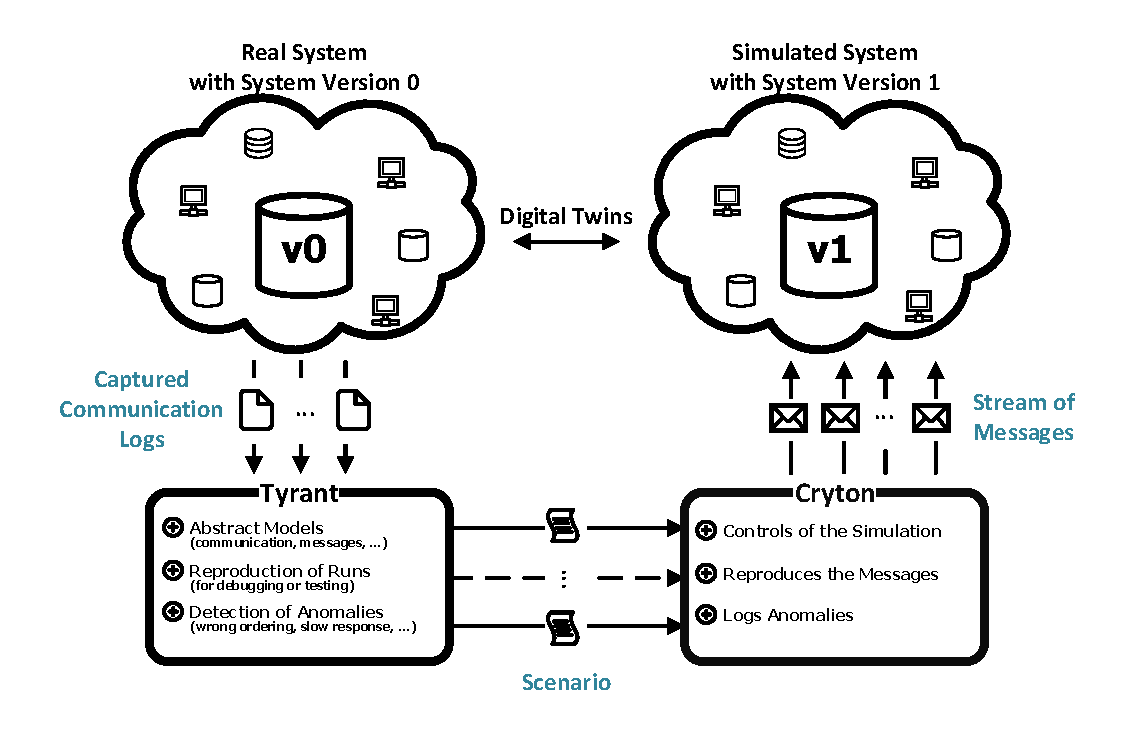
\includegraphics[scale=0.8]{figs/eurocast-diagram.pdf}
  \caption{Scheme of our solution.}
  \label{fig:tunis-diagram}
\end{figure}

An overview of our framework is shown in Figure~\ref{fig:tunis-diagram}.  
%
Our framework requires logs of communication collected from a~real-world
system, e.g., with an older version of MES system under testing: the collected log
usually represents either expected communication in the system, or a log of
communication that led to some incident.  
%
The log is in form of a~sequence of messages between pairs of communicating
components logged with the timestamps of the communication and the data that
were transferred.
%
We derive two kinds of model based on this log: (1) model of the data
transmitted in the messages, and (2) the model of the whole communication in
the system.
%
To model communication, we convert the log to a~so called event calendar
which provides efficient and direct manipulation with seen messages.
Then, we eventually convert event the calendar to a finite automaton (where
every event is a symbol) which is more abstract representation but provides
options for postprocessing (e.g., by applying length abstraction to generate
new test cases) or analyses (e.g., by searching for particular string
representing an error behaviour).
%
From the derived (abstract) models, we generate a so called scenario: a
sequence of concrete messages that will be sent in a real-world or simulated
environment. 
%
A scenario is later used by a digital twin orchestrator to perform simulation
of real system in digital twin.
%
In our case, we use the Cryton tool~\cite{ref_cryton} to orchestrate simulated
environment. Other orchestrators that conform to our format of scenarios can be
naturally used as well. 
%
% It requires as an input a configuration of a system infrastructure and the
% mentioned the scenario.
%
Finally, based on the result of orchestration developers can observe whether
the new version in a digital twin behaves as expected.

% An outline of the paper is following.  The unified representation of the
% different message format is presented in the section \ref{sec:messages}.  A
% model of whole communication and its derivation is described in Section
% \ref{sec:model}.  In Section \ref{sec:scenario} the final transformation of
% model of communication to a scenario for orchestration of digital twin is
% given.

The framework can also be quite easily extended to support the performance
testing of the digital twins.
%
In particular, we propose to mine selected performance metrics (e.g., among
others, the duration of communications) from the captured logs.
%
The metrics are then used for comparison of runs from different environments or
from different versions to detect, e.g., anomalies in the performance.
%
%We also developed an additional tool called \emph{Prefekt} implementing such
%performance analysis.

\paragraph{Related work.} There has been several different approaches for
modelling communication in manufactory and deriving new test cases.
%
\cite{csight} uses Finite Automata to model the communication in systems,
however, their approach is limited to learning only fixed number of components.
%
Another approach is the process mining~\cite{procmin}, a mature technique for
modelling event based system. We see the technique as not suited well for MES
systems as it analyses one-to-one communications and is restricted to a single
thread per node~\cite{procmindist}.
%
%We would not also get any benefits from transforming our logs to series of
%events as it is required by process mining\tsf{I don't get this}.  
%
Modelling of communication for anomaly detection~\cite{havlena} implements an
approach based on probabilistic automata.  
%
The usual communication in manufactory is, however, mostly deterministic,
hence, no probabilistic transitions are created in derived automaton.  
%
Finally, we can mention approaches of~\cite{prospex,icpn08,wcre09} which are
research prototypes only and possible not mature enough for use case in
real-world distributed systems.

Beside modelling communication we need also to model and generate new messages.
In our use case, the messages are in JSON and XML format.
There are several tools which can generate testing data in the formats.
One of them is \emph{DTM Data Generator for JSON} \cite{ref_dtm} which can
generate testing JSON data having structure defined manually by user
or derived from an example input document.
It supports deriving relations in JSON document and contains domain
specific built-in data generator (e.g., address, phones, or URLs).
Moreover it can also combine more structures to new test cases.
However, the software is proprietary, it is not clear how other
formats than XML would be supported and it does not provide
strong abstraction over the input data which would allow
extrapolation for generating testing data.
Another example of tool for generating input data in JSON is \emph{JSON Schema TestData Generator} \cite{ref_stg}.
The tool is open source but quite simple.
It generates test data based on a given JSON scheme and does not provide
any functionality for deriving relations between data in JSON document
or ability to learn and abstract from a given set of JSON documents.

For generating XML, there two class of approaches.
The first one is based on generating XML according to a given XPath query
(so called category-partition based) \cite{xpath1, xpath2}.
The advantage is ability to change specification easily and so generated data.
However, it is not suitable for our purposes since we want learn syntactic structure
of logged messages, not to write their specification manually.
The second one is based on generating XML documents based on a given XML schema \cite{xmlscheme} instance
which is more close to our needs.
But it does not solve generalization of the same class of message to one generic syntactic structure. 

\section{Modelling Messages} \label{sec:messages} 

In distributed system, components usually communicate through messages.
%
We assume, that each message that was captured in the log has the following
parts: (1) a~timestamp (when the message was sent), (2) data (what was sent),
and, (3) a~type (what kind of message was sent).
%
A~suitable data representation of such messages can be a~challenging task,
especially, when modelling the communication among different components.  
%
The representation should be unified for different kinds of data formats (such
as JSON, XML or YAML), should preserve the original semantics, and should allow
generating new test cases from the observed data (e.g., extrapolating extreme
values from the underlying domains).  

Communication logs usually contain lots of subsets of messages that are
structurally similar to each other and differ only in a certain aspects (mainly
in the data that were sent and the type of the message). Thus, we propose
classification of the messages into a groups of similar messages before creating
abstract models.
%
In particular, we classify the seen messages based on the so called fingerprint
of the message (i.e., the spanning tree of the nested structure with respect to
the fields of the data) and based on the type of the message.
%
The idea is that messages having similar structure (but that differ in, e.g.,
number of items in a list, or values in leaves) should have the same abstract
model.
%
For each such class, we construct an abstract model that represents all seen
messages of the given class.
%
Such a~model can then be used not just to reproduce the communication but also
to create new (potentially unseen) messages, e.g., by generating
syntactically-similar messages. 

We propose to model the messages using the following representation (simplified
for the sake of presentation).
%
%
We assume two types of nodes: (1) a~leaf node is a~quadruple $n =
\nodee{k}{l}{u}{V}$, where $k$ is a key associated with the node (e.g., as in
JSON key-value pairs), $l$ (resp. $u$) is the minimum (resp. maximum) number of
occurrences of the node in the given part of message, and $V$ is the set of all
seen values for the node; and (2) a~composite node is a quadruple $n =
\nodee{k}{l}{u}{N}$, where $k$, $l$, and $u$ are defined the same as previously
and $N$ is a set of child nodes (either leaves or composite).
%
We assume that the root of every message is represented by the
$root$ key.
%
Note that we support also other types of nodes, e.g., the attribute node, used
in XML format, but due to the space constrains we omit their description.

To create abstract models, we process input log message by message (which are in
XML or JSON format). 
%
Atomic values correspond to leaf nodes and composite values (lists,
dictionaries, nested tags) correspond to composite nodes.
%
Further, we will work with predicate $c$ over node $n$ written as $c(n)$
(e.g., representing that node $n$ has a specific key). We denote set of
all possible predicates as $C$.

We define the function \emph{reduce} over a~set of leaves $\{n_1,\ldots,n_m\}$
with the same key $k$ as $\reduceop{\{\nodee{k}{l_1}{u_1}{V_1}$, $\ldots$,
$\nodee{k}{l_n}{u_n}{V_n}\}} = \nodee{k}{\sum_1^n l_i}{\sum_1^n u_i}{$
$\bigcup_1^n V_i}$; similarly,  we define the \emph{reduce} of a~set of
composite nodes $\{n_1,\ldots,n_m\}$ corresponding to a key $k$ as
$\reduceop{\{ \nodee{k}{l_1}{u_1}{N_1}, \ldots, \nodee{k}{l_n}{u_n}{N_n}\}} =
\nodee{k}{\sum_1^n l_i}{\sum_1^n u_i}{\bigcup_1^n N_i}$.  
%
Then, for composite nodes, we define the \emph{group and reduce} function as
$\grpreduceop{\nodee{k}{l}{u}{N},\preds{c}{m}}$ $= \nodee{k}{l}{u}{N'}$, where
$\preds{c}{m}$ are predicates and $N' = \bigcup_1^m \big\{ \reduceop{\{n \in N \mid
c_i(n)\}}\big\}$.
%
Basically, the operation groups the children nodes according to a given
predicate (e.g., it groups children named with the same key), merges their
values and aggregates their occurrences.

Finally, we define the \emph{merge} of two nodes ($\mergeop{n}{n'}$) with the
same key $k$ as follows: (1)
$\mergeop{\nodee{k}{l_1}{u_1}{V_1}}{\nodee{k}{l_2}{u_2}{V_2}} = \nodee{k}{min(l_1,
l_2)}{max(u_1, u_2)}{V_1$ $\cup V_2}$, and (2)
$\mergeop{\nodee{k}{l_1}{u_1}{N_1}}{\nodee{k} {l_2}{u_2}{N_2}} =
\nodee{k}{min(l_1, l_2)}{max(u_1, u_2)}{$ $Merged(N_1,$ $N_2)\ \cup\ Copy(N_1,
N_2)\ \cup\ Copy(N_2, N_1)}$, where $Merged(N,$ $N')$ $= \{\mergeop{n}{n'}\ |\
\exists c \in C \, \exists n \in N \, \exists n' \in N': c(n) \wedge c(n')\}$
and $Copied(N,$ $N') = \{n\ |\ \exists c\in C \, \exists n \in N \, \forall n'
\in N':  c(n) \wedge \neg c(n')\}$.
%
We choose values of minimal and maximal number of occurrences to cover both
nodes.
%
In the composite nodes, we group the children satisfying the same criteria and
recursively merge them.  If there is a child node from $N_1$ (resp. $N_2$) with
no node from $N_2$ (resp. $N_1$) that matches the same criterion the first node
is simply copied to the result.  For simplicity, we assume that a criterion $c$
is satisfied by maximally one node in one subtree. 
%
Finally, for each class and its messages with the root nodes $r_1, \ldots,
r_n$, we compute the final abstract node $n$ representing the class as $n =
\mergeop{\grpreduceop{r_1,\preds{c}{m}}}{\mergeop{\ldots}{\grpreduceop{r_n,\preds{c}{m}}}}$.

% \begin{figure}[t!]
%   \centering
%         \includegraphics[scale=0.6]{figs/abstract-example.pdf}
%         \vspace{-6.00mm}
%   \caption{Simplified illustration of the three main operations. Nodes satisfying the same criterion $c$ have the same color; for the sake of simplicity the number in the node represents the number of occurences of the node. Nodes satisfying the same criterion in the same abstract tree are first grouped, then reduced to single node and finally merged with corresponding reduced node from other abstract tree.}
%         \label{abstract-example}
% \end{figure}

\section{Modelling Communication of Monitored System}
\label{sec:model}

Once we derived the models of messages communicated in a system, we further
learn the communication protocol used in the environment.
%
We first use an intermediate data structure called the \emph{event calendar} to
represent messages in the monitored system where each event corresponds to one
message.
%
The messages are ordered chronologically in the calendar by their timestamps.
%
This way we can represent the communication using different protocols and data
formats in a~unified and regular manner and we are not limited to a
fixed number of components.
That would not be possible with other representations which need predefined
topology of a represented system.
%
The calendar is later used to generate scenario precisely reproducing the learnt
communication by transforming each event to a~single step in a~scenario for
orchestrating digital twin.
%
%AS: podle me zbytecne, uz je ot o 2 odstavce vyse
%The calendar of event is derived by extracting the mentioned information
%from each message communicated in system and creating event representing
%the message.
%Then events are sorted to calendar chronologically by timestamp.

Moreover, we want to generate new test cases allowing to experiment on
scenarios which have not yet been seen but are similar to a real-world
situations.
%
Such scenarios bring sometimes more testing value since they are relatively
easy to generate in contrast to the time demanding process of writing
tests manually.
%
Hence, we propose to transform the event calendar to \emph{finite
automaton} and apply, e.g., length abstraction which over-approximates language
of the automaton.
In the following paragraphs, we define our method in a formal way.
% MH: I don't like mixing things below here and trie abstraction
% (\todo{Check+Confirm:} based on \emph{Group},
%\emph{Reduce}, and \emph{Merge} operations) on the level of particular data
%contained in the leaf nodes or on the level of tree structure.

An event is a~tuple $\E = \evnt$ where $\etyp$ is the type of
communication protocol (i.e., OPC-UA or REST), $\esend$ is the identification
of the sender, $\erec$ is the identification of the receiver, $\etime$ is a
timestamp, and $\emsg$ is an abstract representation of the sent message described in the previous section.
Event calendar $\C$ is a list of events $\C = \caldr{n}$.
%
A~finite automaton is tuple $\A=\aut$ where $Q$ is a finite set of states,
$\alp$ is a finite alphabet, $\transe \subset \states\times \alp \times
\powersetof{\states}$ is a transition relation, $\init\subseteq \states$ is a
set of initial states, $\final\subseteq \states$ is a set of final states.  A
language $\lang$ of automaton $\A$, denoted by $\langof{\A}$, is a subset of
$\Sigma^*$.  A run $\run$ of automaton $\A$ is a sequence of states $\runq{n}$
such that $\forall 1 \leq i \leq n-1: \exists a\in \alp:
\intrans{q_i}{a}{q_{i+1}}$.  A word $w=a_1,\ldots,a_n$ is accepted by the
automaton $\A$
%and belongs to its language $\langof{\A}$ 
iff there is a run $\run=\runq{n+1}$ of $\A$ such that $\forall 1 \leq i \leq n:
\intrans{q_i}{a_i}{q_{i+1}}$ and $q_{n+1}\in \final$.  A language $\langst{q}$ of
a state $q\in \states$ is a set $\{w=a_1,\ldots,a_n\,|\, w\emph{ is accepted by
a run }\rho=q_1,\ldots,q_{n+1} \emph{ such that } q_1\in\init \wedge q_{n+1}\in
\final\}$.

Event calendar $\C=\caldr{n}$ is transformed to a finite automaton
$\calA=\calaut$ as follows: the set of states is
$\calst=\{q_1,\ldots,q_{n+1}\}$, the alphabet $\Sigma$ is obtained by
transforming each event $\E=\evnt$ to an unique symbol $a^\E$ by applying
a~hashing function over $(\etyp,\esend,\erec,\etime)$, i.e., giving away $m$,
the set of initial states is $\calin=\{q_1\}$ and the set of final states is
$\calfi=\{q_{n+1}\}$.  Finally, $\forall 2 \leq i \leq n+1:
(q_{i-1},a^{\E_i},\{q_{i}\})$ is added to $\caltr$.  
%\tsf{What's hashing? (AS: now I'm ok with this)}

In order to create the new scenarios, we need to overapproximate the models. In
particular, we propose to use the length abstraction transforming the automaton
$\A$ to an abstracted automaton $\A^\K$ by merging all states with the same
language with respect to a given length.
%
Formally, a length abstraction over an automaton $\A=\aut$ is an equivalence
relation $\abstrln \subseteq \states\times \states$ such that $(p,p')\in
\abstrln$ iff $\langstabs{p}{n}=\langstabs{p'}{n}$ where $\langstabs{q}{n}=\{w'\,|\, \exists w \in \langst{q}: w' \emph{ is a prefix of w} \wedge \emph{length of } w'
\emph{ is up to } n\}$.
We denote an equivalence class of $q\in\states$ by $\eqclasse{q}.$ An abstracted automaton
$\abstrln(\A)=\abstraut$ is obtained using $\abstrln$ in the following way:
$\abstrst=\{\eqclasse{q}\,|\,q\in\states\}$, for each $\intrans{p}{a}{q}$ there
is $(\eqclasse{p}, a, X) \in \abstrtr$ such that $\eqclasse{q}\in X$, and finally,
$\abstrin=\{\eqclasse{q}\,|\,q\in I\}$ and $\abstrfi=\{\eqclasse{q}\,|\,q\in
F\}$.

The length abstraction overaprroximates language of the original automata, i.e.,
$\langof{\A}\subseteq\langof{\abstrA}$ meaning that there may exist a~word
$w=a_1,\ldots,a_n$ such that $w\in\langof{\abstrA} \wedge w\not\in\langof{\A}$.
Both automata have the same alphabet which was originally derived from a~set of
events.  Therefore, it is possible to convert the word $w$ to series of actual
messages.  Supposing that $w$ is not in the language of the original automaton,
we thus obtain a~series of events not present in the original system that can
be used as a new test case for testing MES system in a~digital twin.

\section{Generating Scenario}
\label{sec:scenario}

Finally, we generate a scenario that will be used for orchestration of the
digital twin of the tested system.
%
We iterate over the event calendar and, for each event, we generate one step in
the scenario.
%
Each step consists of sending messages in the digital twin.
%
The concrete messages sent during the orchestration are generated from the
abstract representation.
%
By default, we support exact replication of the seen communication, however, we
provide also an experimental support for, e.g., generating syntactically or
semantically similar messages.

We implemented our framework in our tool \emph{Tyrant}~\cite{ref_tyrant} which
generates scenarios for the orchestrating tool \emph{Cryton}.
%
Cryton uses as an input a~configuration for creating the digital twin (i.e., a
description of digital twin components) and a~scenario generated by Tyrant in
the YAML format.
%

In the following, we will illustrate the transformation of communication logs
from real system to YAML scenario. We remark, we consider a system consisting
of ERP system, MES system, and manufacturing machines and their corresponding
terminals used by human operators.
%
Listing \ref{list:EMM} shows a message between ERP and MES. The message is
stored in the file \texttt{20211207-125952.xml} which has a timestamp encoded
in its name. The message is in XML format and its semantics is that there are 42
items of Material 1 in stocks. 
%Implicitly we know that it was communicated using REST protocol.
%
%
Listing \ref{list:MMM} shows a message between a machine and MES.  The message
was sent one second after the previous one. The message semantics is that
the value of the node $0$ should be set to $99$ in Machine $001$.
% Again, we know that messages between the machines and MES are communicated
% using OPC-UA protocol.
%
%
Finally, Listing \ref{list:GS} shows a~generated scenario consisting of two
steps.  The first step is executed in (logical) time 0 hours, 0 minutes, 0
seconds: the orchestrator will send a message from ERP to MES using the REST
protocol. The message has the XML data attached.  The second steps are executed
one second after the first step: the orchestrator will send another message
from MES to Machine 001 using OPC-UA protocol.  The message says that a value
of the node with path $0$ should be set to $99$.
%
%The Cryton tool later uses scenario like this to precisely orchestrate a
%digital twin.

\begin{figure}
\begin{lstlisting}[caption=20211207-125952.xml,frame=tlrb,label={list:EMM}]{EMM}
 <DataSource>
  <Data>
    <Name>Material1</Name>
    <Value>42</Value>
  </Data>
 </DataSource> 
\end{lstlisting}
\begin{lstlisting}[caption=MES and Machine message,label={list:MMM},frame=tlrb]{MMM}
 SampleDataTime          ; Value ; Name        ; Path
 2021-12-07 12:59:53.617 ;  99   ; Machine 001 ; 0
\end{lstlisting}

\begin{lstlisting}[caption=Generated scenario,frame=tlrb,label={list:GS}]{GS}
---
timestamps:
- delta:
    seconds: 0
    minutes: 0
    hours: 0
  steps:
  - type: ERP
    host: ERP
    target: MES
    args:
      xml: |-
        <DataSource>
          <Data>
            <Name>Data1</Name>
            <Value>42</Value>
          </Data>
        </DataSource>
- delta:
    seconds: 1
    minutes: 0 
    hours: 0
  steps:
  - type: OPC-UA
    host: MES
    target: Machine 001
    args:
     value: 99
     node: 0
\end{lstlisting}
\caption{}
\end{figure}

We implemented the proposed framework in the tool called the \emph{Tyrant}.  
%
We tested our approach on the captured communication provided by a~partner
company that offers a~MES as their product. We were able to successfully
generate valid scenarios for the Cryton tool which then subsequently
orchestrated a digital twin using our scenarios.
However, our Tyrant is still prototype and it would need extensive collaboration
with the company to deploy it to production.
%
% It is implemented in C\# language and supports as an input a log of
% communication of system and generates scenario in YAML langauge as output.
% \newpage

\section{Conclusion}

In this work, we proposed a~generic framework for orchestrating the digital
twins of distributed systems in manufacturing environments. 
%
The main challenges of generating scenarios suitable for orchestrating digital
twins is finding suitable models for (1) the communication in the systems, and
(2) the actual sent messages during the communications.
%
We proposed to use the simple approach: finite automata for communication and
simple abstract representation for messages.

However, in our experience applying the framework in practice requires much
more effort. 
%
Lots of testing scenarios and components require specific preparation before
the orchestration: e.g., setting of the initial database or sending specific
sequence of (hard-coded) messages to prepare the system that are usually not
being captured in the communication log.
%
Currently, our tool supports a concrete use case in a concrete manufacturing
environment.
%
Hence, extending our solution to a more broader class of manufacturing
environments is our future work.

\chapter{Conclusion and Further Directions}
\label{ch:concl}
The main achieved result in shape analysis is
the application of backward run and counterexample-guided refinement (CEGAR) to shape
analysis based forest automata.
Backward run enables distinguishing between real and spurious (caused by abstraction) counterexamples.
This made reporting of found bugs in program reliable and avoid unnecessary false alarms.
The ability to detect spurious counterexamples is the first building block for CEGAR.
The second one is application of predicate abstraction to domain of forest automata what makes precise refinement possible.
Although the originally used height abstraction can be refined too, it does not guarantee
exclusion of spurious counterexample and therefore does not guarantee termination of verification procedure.
On the other hand, predicate abstraction derives the new predicates from a detected spurious counterexample
what prevents reaching the counterexample again.
This enables verification of a new class of data structures where a set of predicates (derived during CEGAR)
is needed to describe their invariants.
The concrete examples were described in Chapter \ref{ch:asv}.

The second result in shape analysis is the multiple participations of the \forester
tool in software verification competition (SV-COMP).
Although we did not win a medal in any major category we shown that our approach
is able to compete and often superior to the other ones.
\forester where able to soundly verify as the only tool in competition test cases
such as skip list of 2nd and 3rd level, various trees,
and also data structures with relations between nodes (for which we derive predicates using CEGAR).

The final result in automata-based shape analysis is introduction of automata over graphs
with bounded tree width which are inspired by Courcelle's theorem \cite{courcell_graph_2012}.
These automata have expressivity higher than forest automata while keeping
feasible algorithmic properties.
Complexity of entailment between automata is singly exponential which we believe
is suitable for application in practical tests cases once some heuristics will be introduced.

We also participated on new kind of shape analysis based on SMT solving.
The possible shapes of data structures allocated on heap are described by logic formulae over bit
vectors.
Basically, it computes points-to relation between pointers used in program and abstract memory
objects used by analyses to represent heap using SMT solver.
This approach is more straightforward than the automata based ones and enables combination of
shape analysis with other domains such as termination analysis, or domains for integer variables.
On the other, it lacks generality of automata based approaches and currently supports
only analysis of linked list data structures.

The second field of focus of the thesis was automated testing.
We developed automated testing procedure for manufacturing execution systems (MES)
in environment of digital twins.
We learn a model of communication protocol and messages sent between software components
of a manufactory where MES is deployed.
We automatically create test scenarios for digital twins using the learnt models
where manufactory is emulated and MES deployed natively.
Since we use finite automata to model communication protocol we can use abstraction to
overapproximate language and create the new test cases.
We can test e.g., a new version of MES before it is deployed to a real manufactory using the described method.
The results of this part of the thesis are mainly from a field of applied research.
We implemented the procedure in the tool Tyrant \cite{ref_tyrant} which was later applied
in Unis company.

\section{Future Directions}
The main potential in automata based shape analysis is in further development
of graph automata over graphs with bounded tree width.
We only sketched the basic concepts and it is needed to design and prove the algorithm
for entailment between automata.
Then one can think about using the formalism in a verification procedure such as
regular model checking or abstract interpretation.
Finally, it is needed to implement the concepts and evaluate it e.g., on SV-COMP
benchmark.
Eventually, design of heuristic for algorithm manipulating these automata may be
an interesting research direction to make the verification procedure work for
difficult test cases.

We would also like to apply collected experience in application of finite automata
in a development of a new automata library.
The library should provide an efficient methods for
manipulation with finite automata.
The crucial algorithms for formal verification and automated reasoning
such as emptiness check or language inclusion checking will be implemented
with various heuristics to make them computationally feasible.
We want to keep library user friendly.
The interface should be simple enough to be usable by anyone with basic
programming skills and knowledge of automata theory.
The source code should hide complicated heuristics and optimizations
and keep basic data structures simple and easily extensible.
The implementation should be in efficient language such as C++ and provide
an interface to a high level programming language.

So far, we implemented the first prototype of library.
It is in C++ and contains efficient representation of finite automata
together with the algorithms over them such as union, intersection,
complementation, determinisation, simulation based reduction, or language inclusion checking.
We further extended the library by finite alternating automata representation.
An interface for Python was implemented over the efficient implementation in C++.
We design a text based format for description of various version of finite automata.
The format support a finite automata and alternating finite automata with explicit, symbolic,
or bitvector alphabet as well as transducers with mentioned alphabets.
The library was already used for development of a new decision procedure for string solving.


In the field of automated testing, one may consider more domain specific abstractions
over model of communication to enable generating more useful test automatically.
There are often domain dependent particularities such as an order of messages sent
in system during initialization or a special restriction of parameters of some
messages.
In current settings, we do not take that in consideration which may lead to
generating scenarios for digital twin which fail early not due to a found bug
in system under testing but because of e.g, wrong initialization of MES.\

\section{Publications Related to this Thesis}
%=========================================================================
The work described in this thesis was published in the following papers.
The backward run and counterexample-guided refinement was published in \cite{vmcai17}.
A paper describing the whole verification procedure based on forest automata
was accepted for publication in book about state-of-the-art verification tool which
should be published in year 2023.
The papers related to \forester participation in SV-COMP are \cite{svcomp15-forester,holik_run_2016,holik_forester_2017}.
Graphs over automata with bounded tree width was sketched in \cite{netys21}.
The approach to shape analysis based on SMT was published in \cite{fmcad18, svcomp-2ls}.

During work on this thesis we participated also on another results related to the shape
analysis which was not included in the thesis.
It was connecting Symbiotic, a static analyser based on symbolic execution, with
Predator, a successful shape analyser using symbolic memory graphs \cite{svcomp-symbiotic}.
Predator won multiple editions of SV-COMP in memory safety related categories and was
therefore a good candidate for providing information about memory safety invariants
for each line of an analysed program.
The information was further used by Symbiotic which relies heavily on slicing of program
over which a symbolic execution is executed.
Particularly, Symbiotic does not need to analyse lines of code which were denoted 
safe (from perspective of memory safety) by Predator executed in overapproximating (sound) mode.
If Predator find a bug in program, Symbiotic takes a bug report and combines it with the
results of its own static pointer analysis to filter out some spurious counterexamples.
The viability of the approach was shown by the second place of Symbiotic and Predator
combination in the memory safety category of SV-COMP 2018.
However, the first place was taken by Predator Hunting Party,
a tool suite of different versions of Predator (one in sound mode, several instances in
bug hunting mode) running on GCC frontend which was more matured than LLVM fronted
used in integration with Symbiotic.
In the next editions of competition, the developers of both tools managed to make LLVM fronted
for Predator as matured as GCC one what resulted to win of Symbiotic in the Memory Safety category.

The work on automated testing is accepted for publication in the proceedings of the conference EUROCAST 2022
which should be published during year 2023.
